\documentclass[oneside,12pt,a4paper]{oucethesis}

% put all the other packages here:
\usepackage{notmystyle}

\begin{document}

% Styles for frontmatter entries in toc
\titlecontents{chapter}[0em]
{\filright}{}{\scshape}
{\titlerule*[1em]{.}\contentspage}

\maketitle

% insert a blank page right after title page (look nicer)
\newpage

\thispagestyle{empty}

\vfil\null

\begin{center}
  \bigskip
  \vspace{1.0in}
  \bigskip
\end{center}

\vfil\null


\frontmatter

\begin{singlespace}
\pagestyle{plain}
\begin{abstract}
\phantomsection % required for using hyperref
\addcontentsline{toc}{chapter}{\abstractname}
% Word limit: 300
\noindent
%Soil is one of the essentials for life on Earth, together with water, air
%and sunlight. Undoubtedly, soil is an important resource for the survival
%of the human race as most agricultural products are cultivated in soil.
%Sustaining agriculturally optimal soil conditions is therefore a crucial
%issue, particularly where soil nutrients, which control crop yields, fibre
%and fuel, are scarce. Globally, soil erosion by water is a serious
%environmental problem. One of many approaches to study this problem is to
%simulate soil erosion using computer models, which help one to understand
%complex interactions between various conditions of land use, soil types and
%climate.
%
%Previously published simulation studies of the effects of future climate
%change upon erosion indicate that, under land usages that leaves the soil
%unprotected, even minor increases in rainfall amounts are likely to result
%in disproportionately large increases in erosion. Such studies, however,
%invariably make the simplifying assumption that distributions of future
%rainfall intensities remain unchanged from the present. This is unlikely to
%be the case. In the latest IPCC (Intergovernmental Panel on Climate Change)
%report, global average water vapour concentration and precipitation are
%projected to increase during the 21st century. This implies that there will
%be an increase in the frequency and magnitude of heavy rainfall. Future
%climate change will certainly affect rainfall intensities, and thus soil
%erosion, but our ability to forecast how future rainfall intensities will
%change is limited by the shortcomings of GCMs (General Circulation Models).
%
%This research aims to understand the effects of rainfall-intensity changes
%caused by climate change on soil erosion by water. Firstly, current trends
%of observed rainfall intensity changes are analysed in order to anticipate
%future rainfall intensity changes. Secondly, the rainfall intensity
%information required for soil erosion estimation is determined. Thirdly,
%this research investigates the implications of rainfall intensity changes
%on soil erosion using computerized models. Lastly, this thesis attempts to
%estimate future rates of soil erosion caused by future rainfall intensity
%changes.
%
%Three observed rainfall datasets---Monthly 0.5\textdegree\ grid data, daily
%station data and tipping-bucket rainfall data---were acquired from South
%Downs, UK. One hundred year-long monthly 0.5\textdegree\ grid data were
%analysed to draw outlines of rainfall amount trends in the study area.
%Trends of daily rainfall amount, number of raindays, simple daily intensity
%index, number of raindays with rainfall amount $\geq$10 mm, and number of
%raindays with rainfall amount $\geq$20 mm were also investigated with 9--93
%year-long daily station data. Then, detailed rainfall-intensity patterns in
%the study area were examined using tipping-bucket gauge rainfall data.
%
%Three process-based erosion models, WEPP (Water Erosion Prediction
%Project), EUROSEM (EURopean Soil Erosion Model), and RillGrow were used to
%simulate runoff and soil loss rates with various rainfall intensities.
%Extreme daily rainfall events with highest rainfall intensity and greatest
%rainfall amount were selected from the tipping-bucket rainfall dataset. The
%storm data were aggregated into predefined time steps ranging from one
%minute to 60 minutes. Runoff and soil losses for these temporally varying
%rainfall data were simulated using three erosion models. The results were
%compared to find out the effects of temporal resolution of rainfall data
%used for simulations of runoff and soil loss. This test determines how the
%scale of rainfall data affects results of erosion modelling.
%
%Effects of rainfall-intensity patterns within storms were studied using
%design storms which have increasing, decreasing, peak-in-the-middle and
%constant intensities, respectively. All storms have the same rainfall
%amount. This provides insights into the responses of erosion models to the
%changes of rainfall intensity pattern within a storm. This, in turn, gives
%better understandings of the effects of rainfall intensity changes during a
%storm on soil erosion by water in reality. An additional daily rainfall
%event with ``intra-storm gaps'' was selected. Runoff and soil loss were
%simulated twice using the event data with ``intra-storm gaps'' and without
%the gaps by removing the ``no-rain'' phase. This examines effects of
%``intra-storm gaps'' within single storm event on soil erosion. Limitations
%of current soil erosion models for incorporating future rainfall intensity
%changes were also discussed.
%
%Future soil erosion rates were estimated using WEPP. One hundred year-long
%weather was generated using CLIGEN (Climate Generator designed for WEPP) as
%reference weather data. Future rainfall-intensity changes were anticipated
%by proportionally changing rainfall intensity related parameters in CLIGEN
%input file. No corresponding rainfall amount change is considered. This
%provides limited but vital information on future soil erosion trends which
%are affected by rainfall intensity changes.

%Soil is one of the essentials for life on Earth, together with water, air
%and sunlight. Undoubtedly, soil is an important resource for the survival
%of the human race as most agricultural products are cultivated on soil.
%Sustaining soil conditions is therefore a crucial issue where soil
%nutrients, which control crop yields, fibre and fuel, are scarce.
Existing simulation studies of the effects of future climate change upon erosion
indicate that, under land usages that leave the soil unprotected, even minor
increases in rainfall amounts are likely to result in disproportionately large
increases in erosion, but make the simplifying assumption that distributions of
future rainfall intensities remain unchanged from the present. This research
aims to determine implications of rainfall-intensity changes on soil erosion
using computerised models. Thus, this thesis is a step towards the ultimate goal
of predicting future rates of soil erosion caused by future rainfall intensity
changes.
%
Three soil erosion models, WEPP, EUROSEM, and RillGrow are employed to
investigate impacts of various rainfall intensities on runoff and soil loss
rates. Two extreme daily rainfall events in summer and autumn are subjectively
selected from the tipping-bucket rainfall data, and runoff and soil losses are
simulated using three erosion models. Estimated runoff and soil loss rates with
high resolution rainfall data are greater than those with low temporal
resolution rainfall data. WSIPs (Within-Storm Intensity Patterns) affect soil
erosion amount, although runoff was not much affected. An additional daily
rainfall event with WSPs (Within-Storm Pauses) within a storm is also selected
to highlight effects of intra-storm pause within a storm on soil erosion.
For a given depth of rainfall, events with constant low intensity produced
dramatically less erosion: thus it appears that assuming a constant (or
averaged) intensity throughout a storm does not provide a good representation of
natural rainfall with its continuously varying intensity.
Analyses of outputs from WEPP simulations reveal a problem that WEPP modifies
original rainfall intensity and, thus, simulates erroneous runoff and erosion
rates.
%
Analysis of three observational rainfall datasets (i.e.\ Monthly 0.5\textdegree\
grid data, daily station data and tipping-bucket gauge data) from the South
Downs, UK show increases in frequency of extreme events, and an increasing trend
in daily rainfall intensity for the future. Future soil erosion rates are
estimated using WEPP and CLIGEN (Climate Generator). 30 year-long weather is
generated by CLIGEN. Likely future rainfall frequency and intensity are
anticipated by changing the mean maximum 30 minutes peak intensity. No future
rainfall amount change is assumed. WEPP simulation results suggest that where
mean maximum 30-min peak intensity of the wet months increases soil erosion
increases at a greater rate than runoff.
%
%Several further investigations are suggested on: Measurement of runoff and
%soil loss with discontinuous storms and their implications for soil
%erosion; An investigation on relationships between duration of no-rain
%period and soil erosion; Development of an erosion model that can fulfil
%the requirements suggested in this thesis; An investigation on the
%relationship of intra-storm intensity patterns and data scale (temporal and
%spatial); An investigation on the trend of intra-storm intensity and
%no-rain periods.
\end{abstract}

%\begin{abstractseparate}
\phantomsection % required for using hyperref
\addcontentsline{toc}{chapter}{Extended Abstract}
%Word limit: 1500
\noindent
%Soil is one of the essentials for life on Earth, together with water, air
%and sunlight. Undoubtedly, soil is an important resource for the survival
%of the human race as most agricultural products are cultivated on soil.
%Sustaining soil conditions is therefore a crucial issue where soil
%nutrients, which control crop yields, fibre and fuel, are scarce.
Globally, soil erosion by water is a serious environmental problem. One of many
approaches to study this problem is to simulate soil erosion using computer
models, which help one to understand complex interactions between various
conditions of land use, soil types and climate.
%
Existing simulation studies of the effects of future climate change upon erosion
indicate that, under land usages that leave the soil unprotected, even minor
increases in rainfall amounts are likely to result in disproportionately large
increases in erosion. Such studies, however, invariably make the simplifying
assumption that distributions of future rainfall intensities remain unchanged
from the present. This is unlikely to be the case. In the latest IPCC
(Intergovernmental Panel on Climate Change) report, global average water vapour
concentration and precipitation are projected to increase during the 21st
century. This implies that there will be an increase in the frequency and
magnitude of heavy rainfall. Future climate change will certainly affect
rainfall intensities, and thus soil erosion, but our ability to forecast future
rainfall intensities is limited by the shortcomings of GCMs (General Circulation
Models).

Therefore, the main objective of this research is to investigate possible
implications of climate change for future erosion with reference to rainfall
intensity changes by analysing the response of erosion models to arbitrary
rainfall intensity changes, and implicitly the process understanding on which
the models are based.
Thus, this research is a step towards the ultimate goal of predicting future
rates of soil erosion caused by future rainfall intensity changes.

Three soil erosion models, WEPP, EUROSEM, and RillGrow are employed to
investigate impacts of various rainfall intensities on runoff and soil loss
rates. Two extreme daily rainfall events in summer and autumn are subjectively
selected from the tipping-bucket rainfall data, and runoff and soil losses are
simulated using three erosion models. Modelling soil erosion requires highly
detailed rainfall-intensity information. Estimated runoff and soil loss rates
with high resolution rainfall data are greater than those with low temporal
resolution rainfall data. WSIPs (Within-Storm Intensity Patterns) affect soil
erosion amount, although runoff was not much affected. An additional daily
rainfall event with WSGs (Within-Storm Gaps) within a storm is also selected to
highlight effects of intra-storm pause within a storm on soil erosion.
For a given depth of rainfall, events with constant low intensity produced
dramatically less erosion: thus it appears that assuming a constant (or
averaged) intensity throughout a storm does not provide a good representation of
natural rainfall with its continuously varying intensity.
Analyses of outputs from WEPP simulations reveal a problem that WEPP modifies
original rainfall intensity and, thus, simulates erroneous runoff and erosion
rates.

Monthly 0.5\textdegree\ grid data for 100 years are analysed to draw outlines of
rainfall trends in the study area. Trends of daily rainfall amount, number of
raindays, simple daily intensity index, number of raindays with rainfall amount
$\geq$10 mm, and number of raindays with rainfall amount $\geq$20 mm are also
investigated with 9--93 years long daily station data. Detailed
rainfall-intensity patterns in the study area are examined using tipping-bucket
rainfall gauge data. Analysis of three observational rainfall datasets show
increases in frequency of extreme events, and an increasing trend in daily
rainfall intensity for the future.
Long-term monthly 0.5\textdegree\ grid data analysis shows a statistically
significant decreasing trend in July rainfall amount over the 1901--2000 period.
With daily observational data, March rainfall amounts in the last two decades
and July rainfall amounts in the last decade show a downward trend although
these are not significant.  Simultaneously, the numbers of raindays per month
show downward trends. Annual daily rainfall-intensity over 1904--1996 has
increased significantly. This is mainly the result of an increased number of
extreme rainfall events ($\geq$10 mm) compared to an annual number of raindays.

Future soil erosion rates are estimated using WEPP and CLIGEN (Climate
Generator). 30 year-long weather is generated by CLIGEN. Likely future rainfall
frequency and intensity are anticipated by changing the mean maximum 30 minutes
peak intensity. No future rainfall amount change is assumed. WEPP simulation
results suggest that where mean maximum 30-min peak intensity of the wet months
increases soil erosion increases at a greater rate than runoff.

Several further investigations are suggested on: measurement of runoff and soil
loss with discontinuous storms and their implications for soil erosion; an
investigation of relationships between duration of no-rain period and soil
erosion; development of an erosion model that can fulfil the requirements
suggested in this thesis; an investigation of the relationship of intra-storm
intensity patterns and data resolution (temporal and spatial); an investigation of
the trend of intra-storm intensity and no-rain periods.
%Storm patterns result in varying simulated runoff and soil loss although
%the simulation results are rather different from measured runoff and soil
%loss. It is evident that storm pattern is an important affecting factor of
%soil erosion modelling.  Inter-storm gaps within a storm also play an
%important role in soil erosion modelling. Discarding inter-storm gaps
%within a storm for soil erosion modelling results in considerable
%overestimation of runoff and soil loss as rainfall duration is effectively
%shortened.
\end{abstractseparate}

\begin{acknowledgements}
\phantomsection % required for using hyperref
\addcontentsline{toc}{chapter}{Acknowledgements}

% God
% David Favis-Mortlock, John Boardman, Richard Washington
% Brenda Boardman
% inspirational Arlin Nicks
% Bofu Yu, Mark New, Mark Nearing
% Environmental Agency (Mr. Russell Long)
% Geoff Calvert & Mike Jackson
% Parents & Parents-in-laws
% Jung Ah
% All who prey for me
\end{acknowledgements}
\begin{dedication}
\texttt{To my loving wife,}\\
\texttt{Lily}
\end{dedication}

\tableofcontents
\listoffigures
\listoftables
\end{singlespace}

%%% adjust paragraph spaces
\addtolength{\footskip}{2ex}
\addtolength{\parskip}{1.5ex}% plus 0.5ex minus 0.2ex}

%Normal Chapter styles in toc
\titlecontents{chapter}[0em]
{\addvspace{4ex} \filright \bfseries}{CHAPTER \thecontentslabel\\}{}
{\titlerule*[1pc]{}\contentspage}

\mainmatter

\part{Introduction}
\label{sec:INTRODUCTION}
%\linenumbers*
\chapter{THE PROBLEM IN CONTEXT}
\label{sec:PROBLEMINTHECONTEXT}

\section{Introduction}
\label{sec:Rationale}
Soil is an important resource for the survival of the human race and is a
central component of environmental systems, together with water, air and
radiation from the sun. Undoubtedly, soil is one of the essentials for life on
Earth. Scientists have investigated various soil properties to ensure good
yields of crops, fibre and fuel \citep{cresser1993-192}. However, soils do not
necessarily always provide ideal conditions for plant growth. Many soil
processes can constrain plant growth: soil hydrology is fundamental for most of
these \citep{hudson1971-320, evans1980-mechanics, kirkby1980-1,
morgan1995-soil}. Among the most serious is soil erosion by water.

Globally, soil erosion by water is a serious present-day environmental problem
and its consequence is subject to extensive investigations
\citep{kirkby1980-1,morgan1995-soil}. Previously published simulation studies of
the effects of future climate change upon erosion indicate that, under land
usages that leave the soil unprotected, even minor increases in rainfall amounts
are likely to result in disproportionately large increases in erosion
\citep{kirkby1980-1, favis1995-365}.

Soil erosion rates may be expected to change in response to changes in climate
for a variety of reasons, the most direct of which is the change in the erosive
power of rainfall
\citep{favis1996-529,williams1996-381,favis1999-329,nearing2001-229,
pruski2002-climate}.
%Soil erosion responds both to the total amount of rainfall and to
%differences in rainfall intensity, however in some situations (e.g. when
%soil is already saturated) the dominant factor appears to be rainfall
%intensity and energy rather than rainfall amount alone.
Existing studies however almost invariably make the simplifying assumption that
distributions of future rainfall intensities remain unchanged from the present
\citep{favis1995-265,favis1995-365}. This is unlikely to be the case.
Intensities may change and/or the frequency of occurrence of high-intensity
events may change \citep{houghton1996-climate, watson1998-517}. Any increases in
the occurrence of high-intensity rainfall---even without any associated
increases in rainfall amounts---may well increase runoff, and hence erosion
rates \citep{kirkby1980-1, morgan1995-soil, parsons2000-723}. Thus, future
climate change will certainly affect rainfall intensities but our ability to
forecast future intensities is limited by the shortcomings of General
Circulation Models (GCMs) \citep{favis1995-365}.

Very few studies have attempted to quantify impacts of changes in future
rainfall intensity \citep{ipcc2001-1032}. Results from these few studies suggest
that more (or similar) rainfall than at present will occur on fewer
raindays---implying an increase in the frequency of heavy rainfall amounts
\citep{watson1998-517}. If these predictions are correct, the implication for
future erosion rates are clear.

For these reasons, there is a urgent need for greater understanding of future
rainfall intensity changes in order to improve the ability of soil erosion
prediction.

\section{Soil Erosion Processes}
\label{sec:SoilErosionProcesses}

\subsection{Introduction}
\label{sec:ErosionProcessesIntroduction}

\begin{quote}
  \begin{quote}
    ``Erosion by water is the redistribution and removal of the
upper layers of the soil, both by the action of falling rain, and by water
flowing over the soil during and after rain or following snowmelt.''
\citep{favis-mortlock2002-452}
  \end{quote}
\end{quote}

The erosion of soil by water and wind is a naturally occurring process, which is
commonly accelerated by human activity. However, when soil erosion occurs at a
greater rate than the rate of soil formation, soil erosion is considered as an
environmental problem. Soil erosion is a ubiquitous problem that threatens an
important and non-renewable resource such as the agricultural land that is
suitable for cultivation (on-site impact) \citep{boardman2003-176}. In addition
to removing a valuable resource, soil erosion leads to increased sediment input
to nearby watercourses, resulting in, for example, the silting-up of dams and
contamination of drinking water (off-site impact)
\citep{mejia1994-331,kitchen1998-179}.

Soil erosion problems can be viewed in three different ways
\citep{kirkby1980-312}. Firstly, in the broadest view, soil erosion can be
compared with other processes of landscape denudation. When and where it is the
most rapid process, soil erosion should be recognised as the dominant problem.
This view leads to the question of what erosion rates can be tolerated in the
long-term. Secondly, a narrower overview examines soil erosion with its
immediate climatic and vegetational controls. This then leads to the question as
to how well the processes involved in raindrop impact, flow generation, and
sediment resistance are understood. Thirdly, soil erosion can be considered in
relation to its broad patterns in time and space. However, the reasons for the
temporal and spatial distributions of soil erosion are only partially understood
\citep{quine2002-55,gomez2005-143,wakiyama2010-993}.

Soil erosion by water is most active where rainfall cannot infiltrate the soil,
but flows over the surface. As the flow travels down a hillslope, it is able to
carry soil materials away mainly by shear stress although other sub-processes
also contribute \citep[see also Figure
\ref{fig:kinnell}]{kinnell2000-discourse,kinnell2005-2815}. In some
cases, only an hour or two of contact time with the surface soil is needed to
carry away an appreciable amount of material. Thus, where overland flow is
dominant, soil erosion by water is likely to be the main process of landscape
denudation. When a large depth of water flows rapidly over the surface with
correspondingly large hydraulic forces, soil erosion acts catastrophically.
These conditions are most commonly found in semi-arid areas, but fields cleared
for agricultural purposes are also subjected to erosion in almost any climate,
which can on occasion be severe \citep{boardman2001-346,boardman2003-176}.

Semi-arid areas are very sensitive to small natural changes in climate and in
such areas it is difficult to separate natural from man-induced changes in
erosion rates. However, even in temperate-humid areas increased erosion
resulting from farming can be sensitively dependent on the extent of the change
in vegetation cover, the total rainfall at periods of low cover, and the
intensity of the rains.

Therefore, two distinct types of area appear to be at great risk of soil
erosion. The first are semi-arid areas, and the second are locations in
temperate areas that have been stripped of vegetation for crop cultivation. A
soil erosion rate can reach at its maximum where intense rainfall occurs during
the period of lowest vegetation cover. This is normally the case in semi-arid
climates or in temperate areas which have been left bare at the time of the
heaviest annual rainfall. In such cases, when the rainfall increases, soil loss
increases, so that the erosional peak tends to be synchronised with the rainfall
peak and this relationship becomes more distinctive when the soil becomes more
unprotected.

When soil erosion problem is to considered, it also is worthwhile to take
long-term effects of soil erosion into consideration. For example, when soil
erosion occurs at a rate of one millimetre per year, it might not have apparent
effect in a human lifetime. However, over a longer-term, the effect can be
considerable. To put this into perspective, topsoil of 15 cm thickness in
general would be completely removed after 150 years if erosion rates stay as
high as 1 mm/year in average with no additional soil formation in the area.
Topsoil contains a high proportion of soil organic matter and the finer mineral
fractions, which provide water and nutrient supplies for plant growth. This may
look as an oversimplification of the erosion process and soil formation, but it
gives us an idea of the long-term effect of soil erosion.

%When soil erosion occurs at a rate of, for example, one millimetre per year, it
%might have little apparent effect in a human lifetime. However, over a
%longer-term, effects can be considerable. This is because erosion continually
%removes the topsoil (e.g., topsoil of 15 cm thickness would be completely
%removed after 150 years if erosion rates are higher as 1 mm/year without
%renewal) which contains a high proportion of soil organic matter and the finer
%mineral fractions, which provide water and nutrient supplies for plant growth.

\subsection{Rainfall}
\label{sec:RainfallCharacteristics}

\subsubsection{Raindrop Splash}
% Raindrop Impact Induced Erosion (need to put more appropriate title)
\label{sec:RaindropSplash}

The process of erosion by water is a two-phase process: detachment and transport
\citep{morgan1995-soil}. Individual soil particles are detached from the soil
mass by the impact of raindrops. The erosive power of raindrops weakens and
loosens the soil surface, and flowing water transports the soil particles
\citep{kinnell2000-discourse}. When sufficient transporting energy is no longer
available, a third phase, deposition, can occur.

\begin{figure}[htbp]
  \centering
  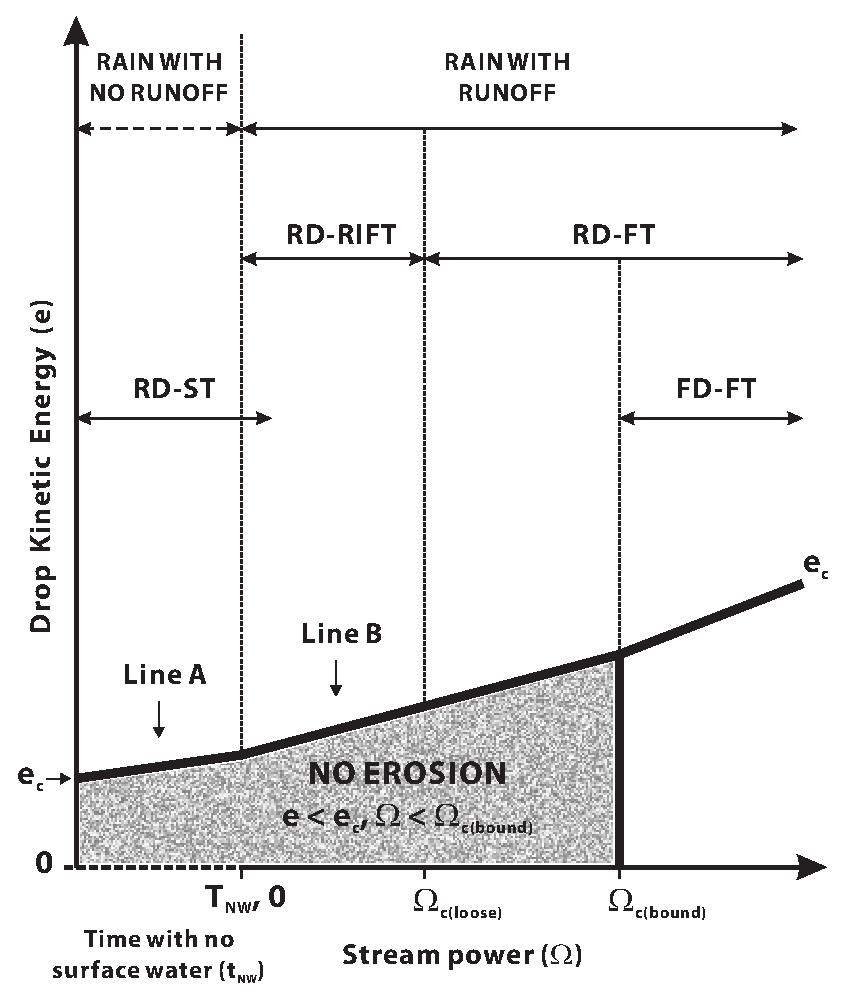
\includegraphics[width=0.70\textwidth]{./img/kinnell}
  \caption[Detachment and transport processes]{Detachment and transport
processes associated with variations in raindrop and flow energies. $T_{NW}$:\
total time when rain falls and there is no surface water. $e_c$:\ critical
raindrop energy to cause detachment; raindrop-induced erosion occurs when drop
energy is equal or greater than $e_c$. Line A:\ $e_c$ when raindrops are
detaching soil particles from the soil surface prior to flow developing. The
slope on this line is used to indicate increasing resistance to detachment
caused by, for example, crust development. Line B:\ $e_c$ when raindrops are
detaching soil particles from the soil surface when flow has developed. The
slope on this line is used to indicate increasing utilization of raindrop energy
in penetrating the flow when flow depth increases as flow power increases.
$\Omega_{c\textrm{(loose)}}$:\ critical stream power required to transport loose
(pre-detached) soil particles. $\Omega_{c\textrm{(bound)}}$:\ critical stream
power required to detach particles bound within the soil surface (held by
cohesion and interparticle friction). RD-ST:\ raindrop detachment and splash
transport. RD-RIFT:\ raindrop detachment and raindrop-induced flow transport.
RD-FT:\ raindrop detachment and flow transport. FD-FT:\ flow detachment and flow
transport\citep[From][]{kinnell2005-2815}.}
  \label{fig:kinnell}
\end{figure}

Raindrop splash distributes soil particles radially away from the site of
detachment. The raindrop detachment-splash transport (RD-ST in Figure
\ref{fig:kinnell}) process is effective where rainfall intensities are high, for
example, as a result of convective rainstorms. However, splash transport (ST) is
a generally inefficient transport mechanism. If the soil has virtually no slope,
soil particles splashed away from the point of impact are replaced by soil
particles detached by other raindrops in the surrounding area
\citep{kinnell2000-discourse,zartl2001-25}. Even if the soil surface has a
slope, net downslope transport by raindrop splash alone is generally small
\citep{kinnell2001-749}.

When water flows start to build up, the soil surface becomes protected from
direct raindrop impact, and another transport mechanism begins to dominate.
Raindrops with sufficient kinetic energy to penetrate through the flow may
detach and lift soil particles into the flow, which then carries them downstream
until it loses sufficient transporting energy to carry the particles. Soil
particles transported by the flow then fall back to the soil surface of lower
grounds. This transport process is termed Raindrop-Induced Flow Transport (RIFT
in Figure \ref{fig:kinnell}) \citep{kinnell1990-497}. While RIFT is more
efficient than ST, it still requires numerous raindrop impacts to move soil
particles downstream.

As rain continues, thin surface water flows become capable of moving loose soil
material on the top of the surface, but might not be capable of detaching soil
material from the soil mass. In many cases, soil particles are detached by the
help of raindrop impacts, and carried away downstream without the need for
raindrops to be involved in the transport process. This raindrop detachment-flow
transport (RD-FT) process is more efficient than RD-RIFT. In a typical field,
both RD-RIFT and RD-FT occur simultaneously in the same flows.

When the critical stream power ($\Omega_{c\textrm{(bound)}}$) for flow to detach
soil particles from soil mass exceeds stream power ($\Omega$), flow detachment
(FD) occurs \citep{kinnell2000-discourse}. Once soil materials are detached and
transported by flow (FD-FT), erosional channels are generated (Figure
\ref{fig:kinnell}). As these channels develop and increase in size to become
large rills and possibly even gullies, processes such as gravitational collapse
of channel walls and heads become important \citep{boardman2003-165}.

\subsubsection{Rainfall Intensity} % Rainfall Intensity Patterns?
\label{sec:RainfallIntensity}

The erosive power of rainfall has long been appreciated by studies on soil
erosion \citep{musgrave1947-133,wischmeier1958-rainfall}. Nevertheless,
obtaining information on rainfall intensity for soil erosion is very much
problematic. One way of measuring rainfall intensity would be measuring size,
distribution and velocity of raindrops, so that the kinetic energy of the
rainfall can be calculated \citep{cerda1997-169,lascelles2000-709}. This can be
seen as a `bottom-up' approach. Another method would be simply to measure
rainfall amount and duration, so that intensity can be obtained by dividing
rainfall amount by duration (i.e. rainfall amount per unit time)
\citep{osborn1998-505}. This is a `top-down' approach. However, both approaches
have their own shortcomings
\citep{parsons2000-723,schuur2001-1019,garcia2001-675}.

Although rainfall intensity plays a very important role for soil erosion, it is
important to recognise that the vital variable for soil erosion by splash is not
rainfall intensity itself, but rainfall energy. This rainfall energy varies in
association with rainfall intensity. As raindrops increase in size, their
terminal velocity increases. This increases the kinetic energy of raindrops. The
total kinetic energy of rainfall also increases with increasing number of
raindrops during a given time. The total kinetic energy of rainfall may be
estimated from the distribution of raindrop size and number of raindrops during
a storm. The accuracy of this estimation is, however, limited by natural
variations in rainfall characteristics \citep{vandijk2002-1}. Yet, in natural
rainfall events, the relationship between rainfall intensity and energy is
neither so clear, nor simple. Despite this, simple assumptions about the
rainfall intensity-energy relationship are often made in studies on soil
erosion, in particular, modelling studies, as rainfall intensity is the
only easily modifiable control on rainfall energy in such studies
\citep{laflen1997-96,morgan1998-389}.

\citet{parsons2006-68} ran a laboratory-based rainfall simulation
experiment to determine the implications of temporal variation of rainfall
intensity for rates of soil loss. He found that erosion is least for the
constant-intensity storms. This is highly significant because soil-erosion
models are typically calibrated using data obtained from constant-intensity
experiments. Moreover, storm pattern does not appear to affect the volume of
runoff, but it does affect the quantity of eroded sediment. In particular, the
constant-intensity storm patterns are associated with low erosion rates. Storm
pattern also affects the size-distribution of the eroded sediment.
\citet{parsons2006-68} therefore concludes that the relationship between
rainfall energy and interrill erosion is more complex than is currently assumed
in process-based models of soil erosion.

Other studies also note that there are complex interactions between raindrop
size, velocity and the duration of rain, which control the erosive power of
rainfall \citep{kinnell1981-153,brandt1990-687,salles1999-545,vandijk2002-1}.

\subsection{Soil Type}
\label{sec:SoilType}

Soil erodibility is an estimate of the resistance of the soil to erosion, based
on the physical characteristics of each soil \citep{morgan1995-soil}. Although
erodibility varies with soil texture, aggregate stability, shear strength,
infiltration capacity and organic and chemical contents, soils with high
infiltration rates, higher levels of organic matter and improved soil structure
have a greater resistance to erosion, in general \citep{morgan1995-soil}.

Erodible soils have restricted clay content \citep{bryan2000-385}. Soils with
more than 30--35\% clay are generally coherent and form stable soil aggregates,
which are resistant to raindrop impact and splash erosion
\citep{evans1980-mechanics}. Clays often have rough surfaces to store much
water, and are resistant to sheet and rill erosion. Sands and coarse loamy
sands, on the other hand, have high infiltration rates and resistant to erosion,
and even if this is exceeded, sands (more than 0.3 mm diameter) are not easily
eroded by flowing water or by raindrop impact
\citep{evans1980-mechanics,marshall1996-soil}.

Sandy soils are however more erodible than clayey soils because the aggregates
of these sandy soils slake more readily and seal the soil surface
\citep{lebissonnais1996-425}. Loamy soils are also particularly at risk of
sealing \citep{ramos2000-398}.

After cultivation, the soil surface becomes rough. The amount of water, which
can be stored on the surface before runoff takes place, is thus large at this
time. Surface roughness is least after drilling and rolling of the seedbed, and
differences between soil types are smallest \citep{robinson1992-151}. For
similar soil types, the timing of cultivation can affect the storage volume, for
example, a clay surface prepared in winter can have more than twice as much
storage volume as a surface prepared in spring \citep{evans1980-mechanics}.

Moreover, stony soils are generally less vulnerable to erosion as the surface
stones not only protect the soil, but also increase infiltration by providing
larger pores between stones
\citep{agassi1991-565,poesen1994-1,defigueiredo1998-81}. However, when rock
fragments are well-embedded in a surface seal, a positive relation for runoff
and sediment yield is found \citep{poesen1992-451}. A negative relation occurs
either where rock fragments are partly embedded in a top layer with structural
porosity or where the rock fragments rest on the surface of a soil having either
textural or structural pore spaces \citep{poesen1992-451}.

\subsection{Topography}
\label{sec:Topography}

There are two aspects of topography that affect erosion: slope angle and length.
Normally, erosion would be expected to increase as the slope steepness increases
\citep{liu1994-1835}. Soil erosion by water also increases as the slope length
increases because of increases in velocity and volume of runoff
\citep{liu2000-1759}. Water depth increases with downslope distance so that
interrill soil erosion is affected by slope length \citep{gilley1985-154}.
Water depth then affects soil detachment and overland flow sediment transport
capacity \citep{gilley1985-147}. Slope angle is also closely related to the
effectiveness of splash erosion \citep{kinnell2000-discourse,vandijk2003-153}.

The location of downslope is an important factor that determines the
development of rills on a hillslope. However, there is another factor that is
closely related to the dynamics of initiation and growth of rills. The
minute variations of soil surface topography, also known as microtopography, can
play an important roll on this ``rill competition''.

Microtopography is not temporally static because erosional processes will
continuously modify the surface of soil during a rainfall event. As a
result, runoff during the latter part of the event will flow over a soil
surface that has been modified and different from the surface earlier in the
rainfall. Thus, erosive modification of microtopography constitutes a feedback
loop which might be expected to operate in a positive sense. The most
`successful' rills (i.e. those conveying the most runoff) will modify the local
microtopography to the greatest extent, and so will most effectively increase
their chances of capturing and conveying subsequent runoff.

\citet{favis-mortlock2000-2173} previously recognised the importance of
microtopography
in the initiation and the development of rills, and developed a erosion model,
RillGrow, using a self-organising dynamic systems approach. More about RillGrow
is included in Section \ref{sec:ModelDescriptionRillGrow}.
%******you need to mention also something about microtopograghy, at the mm to cm
%scale, about how this is important in (among other things) determining the
%location of preferential flow paths and so of rills.

\subsection{Land Use}
\label{sec:LandUse}

Soil erosion potential is highest where the soil has no or very little
vegetative cover. Vegetation cover protects the soil from direct raindrop impact
and splash, and tends to slow down surface runoff. On a field with complete
vegetation cover, runoff and erosion are comparatively small, often less than
5\% of runoff and 1\% of erosion from bare soil, respectively
\citep{braskerud2001-1447,rey2003-549}. One reason is because the infiltration
rates of the vegetated field are relatively higher than those on bare soils as
the field often has a better soil structure and more stable aggregates
\citep{robinson2001-1}. When runoff does take place, the leaves and roots of
plants inhibit the flow by reducing the velocity of the flow
\citep{braskerud2001-1447,rey2003-549}. On soils with less than 70\% vegetation
cover, runoff and erosion increase rapidly when rainfall occurs
\citep{favis-mortlock1996-529}. Under less than 20--30\% vegetation cover,
runoff and erosion are related to the amount of bare ground, increasing as the
proportion of bare ground increases \citep{favis-mortlock1996-529}.

The effectiveness of any crop management system against soil erosion by water
also depends on how much protection is available at various periods during the
year, relative to the rainfall amount that falls during these periods. In this
respect, crops which cover for a major portion of the year (e.g., alfalfa or
winter cover crops) can reduce erosion much more than can crops (e.g., row crops
) which leave the soil bare for a longer period of time and particularly during
periods of intense rainfall \citep{zhang1995-1069,zhang1995-1079}.

%\subsection{Rill and Interrill Erosion}
%\label{sec:RillAndInterrillErosion}
%
%Rills are initiated at a critical distance downslope where overland flow
%becomes channelled.
%
%Interrill erosion is due to detachment and transport by raindrop impact and
%overland flow. Interrill erosion has been shown to be approximately
%proportional to the square of the rainfall intensity \citep{watson1986-97}.
%In addition to rainfall intensity, interrill erosion is related to slope
%\citep{watson1986-97}.

\section{Soil Erosion and Rainfall Intensity}
\label{sec:RainfallIntensityAndSoilErosion}

This section provides examples of some notable erosion events which are
documented in selected publications.



\paragraph{South Downs, East Sussex, UK, October 1987
\citep{boardman1988-333}}
\label{sec:SouthDownsOctober1987}

Heavy rainfall on 7 October 1987 and subsequent storms resulted in soil losses
over 50 m$^3$/ha\ on several fields and over 200 m$^3$/ha\ on one field in the
eastern South Downs \citep{boardman1988-333}. Monthly rainfall totals at
Southover, Lewes, were 54.3 mm for September and 270.9 mm for October 1987.
Rainfall recorded at Southover, Lewes, on 7 October 1987 was 50.2 mm with a
maximum short period intensity of 6.7 mm/h\ for 5.5 hours including 40 mm/h\ for
15 minutes.

Substantial rills or gullies were formed by the rainfall event on 7 October
1987. As a result of this, following rainfalls as low as 7 mm caused runoff and
erosion \citep{boardman1988-333}.
Although there are no event-by-event records available for soil losses, it is
evident that the rainfall on 7 October 1987 played an important role, by
contributing to rill or gully generation, on  soil erosion in the area. However,
the main factors responsible for the severe erosion were land use and farming
practices.

%%%%%
\paragraph{Vicrello, Tuscany, Italy, May 1994 \citep{torri1999-131}}
\label{sec:VicrelloVolterraTuscany}

A rainfall depth of 77.8 mm fell on a field plot with a bare soil in Vicrello,
Tuscany, Italy \citep{torri1999-131}. The storm lasted for over 28 hours and
caused a soil loss of 126.2 t/ha. Maximum intensity averaged over 10 minute was
120 mm/h.

\paragraph{Hadspen, Somerset, UK, May 1998 \citep{clark2000-17}}
\label{sec:HadspenSomersetUK}
Total rainfall amount of 47.6 mm fell in Hadspen, Somerset, UK on 13 May 1998
\citep{clark2000-17}. Most rain fell between 2115 GMT to 2130 GMT reaching
rainfall intensity of $>$100 mm/h. In Nettlecombe Hill and Higher Hadspen,
ploughed fields on slopes with 2--11\textdegree\ eroded 1.412
tonnes/m$^3$ and 1.312 tonnes/m$^3$ as dry bulk density, respectively.
Because of the difficulties involved in measuring soil loss amount directly,
\citet{clark2000-17} took survey to estimate the volume of soil that was cleared
from the site and dumped into a nearby field. Then, samples from soil was taken
and the dry bulk density was determined. Total soil loss from two area was 60.6
tonnes and 11.5 tonnes respectively.

\paragraph{Ashow, Warwickshire, UK, August 1999 \citep{harrison1999-143}}
\label{sec:AshowWarwickshireUK}
On 20 August 1996 in Ashow, Warwickshire, the storm commenced at 1930 BST.
Rainfall intensity was low until 2030 BST when 24.5 mm of rain fell in 30 min
and a total of 33.5 mm fell before midnight.

One of two fields in the catchment was planted with oilseed rape eight days
before the storm. The field was ploughed and power-harrowed, and then seed
drilled with a low ground pressure buggy. It was subsequently rolled by a
tractor with low ground pressure tyres. The other field was harvested of wheat
and barley, and then rough ploughed, the soil clods being broken up using
rotating discs.

Extensive erosion of top soil occurred, followed by the development of gullies
and rills by overland flow during the storm. Approximately 790 tonnes of
sediment was eroded from the two fields excluding the sediment that reached
nearby river (River Avon, UK). Average sediment yields was 49.7 t/ha which is
equivalent to the average ground lowering of 3.8 mm from the site.

\paragraph{Northern Ethiopia Highlands, 1998-2000 \citep{nyssen2005-172}}
\label{sec:NorthernEthiopiaHighlands}

Rainfall intensity in Northern Ethiopia Highlands was monitored using a tipping
bucket rain gauge during 1998-2000 \citep{nyssen2005-172}. Overall rain
intensity in the area is low. 88\% of total rain volume falls with an intensity
$<$30 mm/h. Most storms have a low intensity with a brief high intensity part.
This high intensity can be observed at the beginning, in the middle or at the
end of the storm.

Although area-averaged intensity was low in this area, it was found that maximum
rain intensity at individual locations exceeded by far the threshold values for
excessive rain (see Table 5, \citealp{nyssen2005-172}). Rainfall intensities
beyond these thresholds were known to cause $>$50\% of total soil losses
\citep{krauer1988-rainfallerosivityand}. Large rain erosivity in the area is due
to larger median volume drop diameters ($D_{50}$) than those reported for other
regions of the world, rather than due to high intensity.

Despite the low rainfall intensity, presumably large proportions of soil may
have been lost from the area. The article only implies the erosion event. Also,
no actual soil loss amount was presented.

%%%%%
\paragraph{South Downs, East Sussex, UK, October 2000
\citep{boardman2001-346}}
\label{sec:SouthDownsOctober2000}

Exceptional rainfall in October and November 2000, especially a 24-hour fall of
about 100 mm, led to extensive erosion and property damage
\citep{boardman2001-346}. The rainfall was typical of frontal, low-intensity
events that usually occur in British winters but it lasted for a longer period
than usual period. In a 24-hour period prior to 09:00 on 12 October (i.e.\ 11
October rainday), a total rainfall of 89.9 mm was recorded
\citep{boardman2001-346}.
In a 10-hour period of continuous rainfall (23:00--09:00) 63.8 mm fell with a
maximum intensity of 11.4 mm/h\ and a maximum short-period intensity of 3.6
mm/min\ (i.e.\ 216 mm/hr) \citep{boardman2001-346}.

Rainfall of 100 mm in 24 hours has a return period of well over 100 years and a
intensity of 11 mm/h is to be expected every year \citep{boardman2001-346}. This
means that the rainfall on 11 October 2000 has a rainfall intensity that is
commonly observed in the area, but the total amount and duration are very
unlikely in the area. It is noted that high intensity rainfall within prolonged
low intensity rainfall at the time of year when the agricultural land is most
vulnerable may result in extensive erosion events.

On one field from the studied site, a gully up to 1.5 m deep, 0.5 m wide and
more than 200 m long was cut by runoff on 11 October 2000. Because no erosion
measurement was taken during the rainfall event, total erosion amount is
unknown for the specific event on 11 October 2000 but severe erosion and muddy
flood occurred on the day. 

\paragraph{Synthesis}
The events presented above are few examples of rainfall events that were
followed by soil erosion events. Although they are subjectively selected, this
is not an either comprehensive or limited list.

These cases give an idea of the diversity of soil erosion responses
to different (i.e.\ high or low) rainfall intensities. Severe soil erosion
events do not necessarily always occur with rainfall events with high rainfall
intensity. Rainfall events with low intensity can also produce soil erosion.
This is because sometimes (and quite often) other erosion-affecting factors such
as the timing of a rainfall event may play more important roles than rainfall
intensity. Thus, it would be difficult to compare these events presented in this
section directly in order to identify the effect of rainfall intensity.

Also, these case studies presented here show that studies of rainfall events
that were followed by sever erosion events do not always have measurements for
the erosion. This is an importance issue. The difficulties that arise from
monitoring and modelling soil erosion often start from finding ``right''
observational data. This would be the first obstacle that one may have to face
when doing simulation studies on soil erosion.


\section{Rainfall Intensity and Climate Change}
\label{sec:RainfallIntensityAndClimateChange}

Many studies using GCMs predict an increase in global average precipitation in
response to global warming induced by greenhouse gases
\citep{houghton1996-climate,jones2001-1337,ipcc2001-881,ipcc2001-1032,
ipcc2007-impact,ipcc2007-physical}. This increase in global average
precipitation has been based on the assumption that an increasing global-mean
temperature will intensify the hydrological cycle
\citep{nearing2005-131}. The IPCC reported that there has been a very
likely increase in precipitation during the 20th century in the mid-to-high
latitudes of the Northern Hemisphere \citep{ipcc2001-881,ipcc2007-physical}.
Climate models are also predicting a continued increase in intense precipitation
events during the 21st century \citep{ipcc2001-1032,ipcc2007-impact}.

In addition, there has been a number of investigations using observed data
that provided some evidences for a significant increase in extreme precipitation
\citep{karl1995-217,karl1998-231,osborn2000-347,osborn2002-1313}.
\citet{karl1995-217} and \citet{karl1998-231} observed increases in extreme
precipitation (greater than 50 mm per day) in the United States using historical
data over the period 1910--1996. \citet{osborn2000-347} and
\citet{osborn2002-1313} also observed an increasing trend in intense daily
precipitation over the period 1961--2000 in the United Kingdom. They found that,
on average, precipitations were becoming more intense in winter and less intense
in summer.

The findings by \citet{osborn2000-347} and \citet{osborn2002-1313} are generally
consistent with the results from the GCM simulations
\citep{jones1997-265,jones2001-1337}. However,
\citet{ipcc2001-1032,ipcc2001-881} indicated that potential changes in intense
rainfall frequency are difficult to infer from global climate models, largely
because of coarse spatial resolution. The ability of GCM integrations and
operational analyses to simulate realistic precipitation patterns, spatially and
seasonally, is also generally not as good as the ability to predict temperature
\citep{mcguffie1999-1}. The likelihood of finding real trends in the frequency
of extreme events becomes lower the more extreme the event
\citep{frei2001-1568}. The same authors demonstrate this by applying known
trends in the scale parameter to synthetic data series, and then attempt to
identify statistically significant trends in the frequency of various extreme
events.

%******$Summarise what are those physical reasons in \citealp{trenberth2000-12}.

There are various physical reasons (see \citealp{trenberth2000-12}) why a large
increase in the magnitude of heavy precipitation may occur with only a
correspondingly small increase in mean precipitation. It is even possible that
heavy precipitation occurrence could increase when mean precipitation decreases,
if there is a more radical change in the precipitation distribution
\citep{osborn2002-1313}.

A study by \citet{nearing2001-229} estimated potential changes in rainfall
erosivity in the United States during the 21st century under climate change
scenarios. He concluded that, across the United States over an 80 year
period, the magnitude of average changes in rainfall erosivity was 16--58\%.
This variability in the magnitude was due to the method (two GCM models and
two scenarios) that he used to predict the changes in rainfall erosivity.
Regardless of which method was used, he suggested that changes in erosivity will
be critical at certain locations.

In order to run a soil erosion model such as WEPP (Water Erosion Prediction
Project, See Section \ref{sec:WaterErosionPredictionProjectWEPP} for more
details), for example, various weather parameters for each day of the
simulation period are required \citep{flanagan1995-usda}. These weather
variables (e.g. rainfall depth and duration, peak storm intensity and time to
peak, minimum and maximum temperatures, dew point temperature, solar radiation,
wind speed and direction) can either be generated by CLIGEN (CLImate GENerator,
See Section \ref{sec:ClimateGeneratorCLIGEN} for more details) or compiled
manually from observed climate data.

Generating climate data for studies on future soil erosion is not a simple task,
even with today's climate data, as a starting point, since all erosion
predictions must involve modelling extreme weather events. Extreme weather
events (e.g., heavy showers, gusts and tornadoes) are rare and occur on the
synoptic and even smaller temporal and spatial scales
\citep{schubert1997-223,katz1999-133,coppus2002-1365}. Long integrations of very
high-resolution models are required to simulate those extreme events and even
then, there is little prospect that sub-synoptic scale events can be
successfully resolved in GCMs. GCM grid sizes are too large to properly capture
convective elements in the atmosphere, so that precipitation within a short
period (e.g., one day) is poorly reproduced by GCMs \citep{schubert1997-223}.

There are a few ways for resolving this scale issues with GCM data. One way is
by using climate data generated directly by Regional Climate Models (RCMs) that
are capable of generating climate data with a sub-daily resolution (i.e.
20-min). Another can be achieved by downscaling. There are several approaches
for downscaling GCM data into regional scale. \citet{wilby1997-530} divided
downscaling into four categories: regression methods, weather pattern
(circulation)-based approaches, stochastic weather generators and limited-area
climate models. Among these approaches, circulation-based downscaling methods
perform well in simulating present observed and model-generated daily
precipitation characteristics, but regression methods are preferred because of
its ease of implementation and low computation requirements. RCM data and
downscaled data allow predictions to be made at a finer scale than GCMs. All of
these methods are widely accepted methods that were often chosen to generate
climate data with a sub-daily resolution.
%******this is an important point, see Dave's email on 11/10/09 17:40:17. If
%GCMs cannot reproduce present day rain intensity, how can they be expected to
%give us information about future rain intensity? Say more.

Lastly, \citet{ipcc2001-1032} reported generalised results from the analysis
of five regional climate change simulations. Although scenarios for
precipitation produced by these experiments varied widely among models and from
region to region, the results provide very important working envelopes for this
research. The results related to precipitation are summarised as follows:
\begin{enumerate}
  \item Regional precipitation error spanned a wide range, with values as
extreme as approximately $-$90\% or $+$200\%.
  \item Simulated precipitation sensitivity to doubled CO$_2$ was mostly
in the range of $-$20\% to $+$20\% of the control value.
  \item Overall, the precipitation errors were greater than the simulated
changes. It can be expected that, due to relatively high temporal and spatial
variability in precipitation, temperature changes are more likely to be
statistically significant than precipitation changes.
\end{enumerate}

\section{Soil Erosion Prediction Models}
\label{sec:SoilErosionPredictionModels}

\subsection{Introduction}
\label{sec:Introductionerosionmodels}

To assess the risk of soil erosion, estimates of soil loss rates may be compared
with what is considered to be acceptable for conservation purposes; the effects
of different conservation strategies may then be determined. Consequently, a
technique is required to compare possible soil losses under a wide range of
conditions. One way of doing this is using computerised models for soil erosion,
which are (like all models) simplified representations of reality. Types of
erosion models are categorised by their structures in Table
\ref{tab:TypesOfModels}. It needs to be noted that the categories in Table
\ref{tab:TypesOfModels} tend to be mixed, nowadays.

Another categorisation scheme is based on objectives and levels of performance.
In this scheme, there are two basic types of models in addition to the
categories in Table \ref{tab:TypesOfModels}. One is a screening model, which is
relatively simple and designed to identify problem areas. This type of model
only requires predictions of the right order of magnitude. The other type is an
assessment model, which requires better, more robust, and accurate predictions
because it is mainly designed for evaluating the severity of erosion, for
example, under different soil management systems. Thus, depending on the purpose
to which a model is put, the appropriate level of complexity/simplicity of
the model should be established. A clear statement of the purpose of the study
is essential; this will serve as a starting point for all modelling procedures.

Our current understanding of erosion processes is greatest over short time
periods, seconds to minutes. It is thus problematic when applying this
understanding to longer periods, e.g.\ months to years or even longer, as is
necessary for real-world conservation tasks. It may just be feasible for
slightly longer periods such as hours or days, but continuous extrapolation is
not appropriate \citep{kirkby1992-180,morgan1995-soil}. Therefore, longer-term
prediction can only be achieved by summing the predictions for individual
events, or developing models empirically, using data collected on a long-term
basis, or improving our understanding of processes to be able to build
physically-based models.

\begin{sidewaystable}[htbp]
  \centering
  \caption[Types of models]{Types of models
(from \citealp{morgan1995-soil})}
  \label{tab:TypesOfModels}
    \small
    \begin{tabular}{lp{150.0mm}}
    \toprule
    \textbf{Type} & \textbf{Description}\\
  % \midrule
    Physical & Scaled-down hardware models usually built in the
laboratory; need to assume dynamic similitude between model and real world.\\
    \midrule
    Analogue & Use of mechanical or electrical systems analogous to
system under investigation, e.g. flow of electricity used to simulate flow of
water.\\
    \midrule
    Digital & Based on use of digital computers to process vast
quantities of data.\\
    \midrule
    Physically-based & Based on mathematical equations to describe
the processes involved in the model, taking account of the laws of conservation
of mass and energy.\\
    \midrule
    Stochastic & Based on generating synthetic sequences of data
from the statistical characteristics of existing sample data; useful for
generating input sequences to physically-based and empirical models where data
only available for short period of observation.\\
    \midrule
    Empirical & Based on identifying statistically significant
relationships between assumed important variables where a reasonable database
exists. Three types of analysis are recognised:
    \begin{compactitem}[-]
      \item Black-box: where only main inputs and outputs
are studied;
      \item Grey-box: where some detail of how the system
works is known;
      \item White-box: where all details of how the system
operates are known.
    \end{compactitem}\\
%   \addlinespace[-3.5mm]
    \bottomrule
    \end{tabular}
\end{sidewaystable}

In addition to these temporal extrapolation issues, the spatial extrapolation
issues must also be considered. For instance, the detailed requirements for
modelling erosion over a large drainage basin \citep{hooke2000-1778} may differ
from those demanded by models of soil loss from a short length of hillslope
\citep{goff1993-698}, or even at the point of impact of a single raindrop
\citep{sharma1991-301}. Until recently, integrating researches in different
scales (i.e.\ plot, field and catchment-scale) has been neglected because it is
a difficult task \citep{boardman1996-489}.

Therefore, prior to using a soil erosion model, where the model is to be
used and why the specific model is appropriate should be considered carefully.

For error and uncertainty involved in modelling approaches,
\citet{oberkampf2002-333} suggest two definitions of uncertainty: aleatory and
epistemic.
Aleatory uncertainty refers to irreducible uncertainty, inherent uncertainty,
variability and stochastic uncertainty. A probability or frequency distribution
is generally used to quantify aleatory uncertainty, when sufficient information
is available.
Epistemic uncertainty refers to reducible uncertainty, subjective uncertainty
and cognitive uncertainty. This is a source of non-deterministic behaviour that
comes from lack of knowledge of the system or environment. This uncertainty can
also be viewed as a potential inaccuracy in any phase or activity of the
modelling process that is due to lack of knowledge.

Thus, even if we eliminate epistemic uncertainty by studying and obtain absolute
knowledge, we will still not be able to predict future weather perfectly because
of the aleatory uncertainty.

\citet{oberkampf2002-333} defines error as a recognizable inaccuracy in any
phase or activity of modelling and simulation that is not due to lack of
knowledge. Using this approach, there are two types of errors: errors that are
acknowledged and errors that are unacknowledged. Acknowledged errors are
those inaccuracies that are recognised by the analysts. Unacknowledged errors
are those inaccuracies that are not recognized by the analysts, but they are
recognizable. The CLIGEN errors found by \citet{yu2000-301} can be seen as an
example of unacknowledged errors (See Section \ref{sec:ClimateGeneratorCLIGEN}).

\citet{oberkampf2002-333} further suggest a comprehensive and new view of the
general phases of modelling and simulation, consisting of six phases (Figure
\ref{fig:modelling_phases}):
\begin{enumerate*}
  \item conceptual modelling of the physical system
  \item mathematical modelling of the conceptual model
  \item discretization and algorithm selection for the mathematical model
  \item computer programming of the discrete model
  \item numerical solution of the computer program model
  \item representation of the numerical solution
\end{enumerate*}

\begin{figure}[htpb]
  \centering
    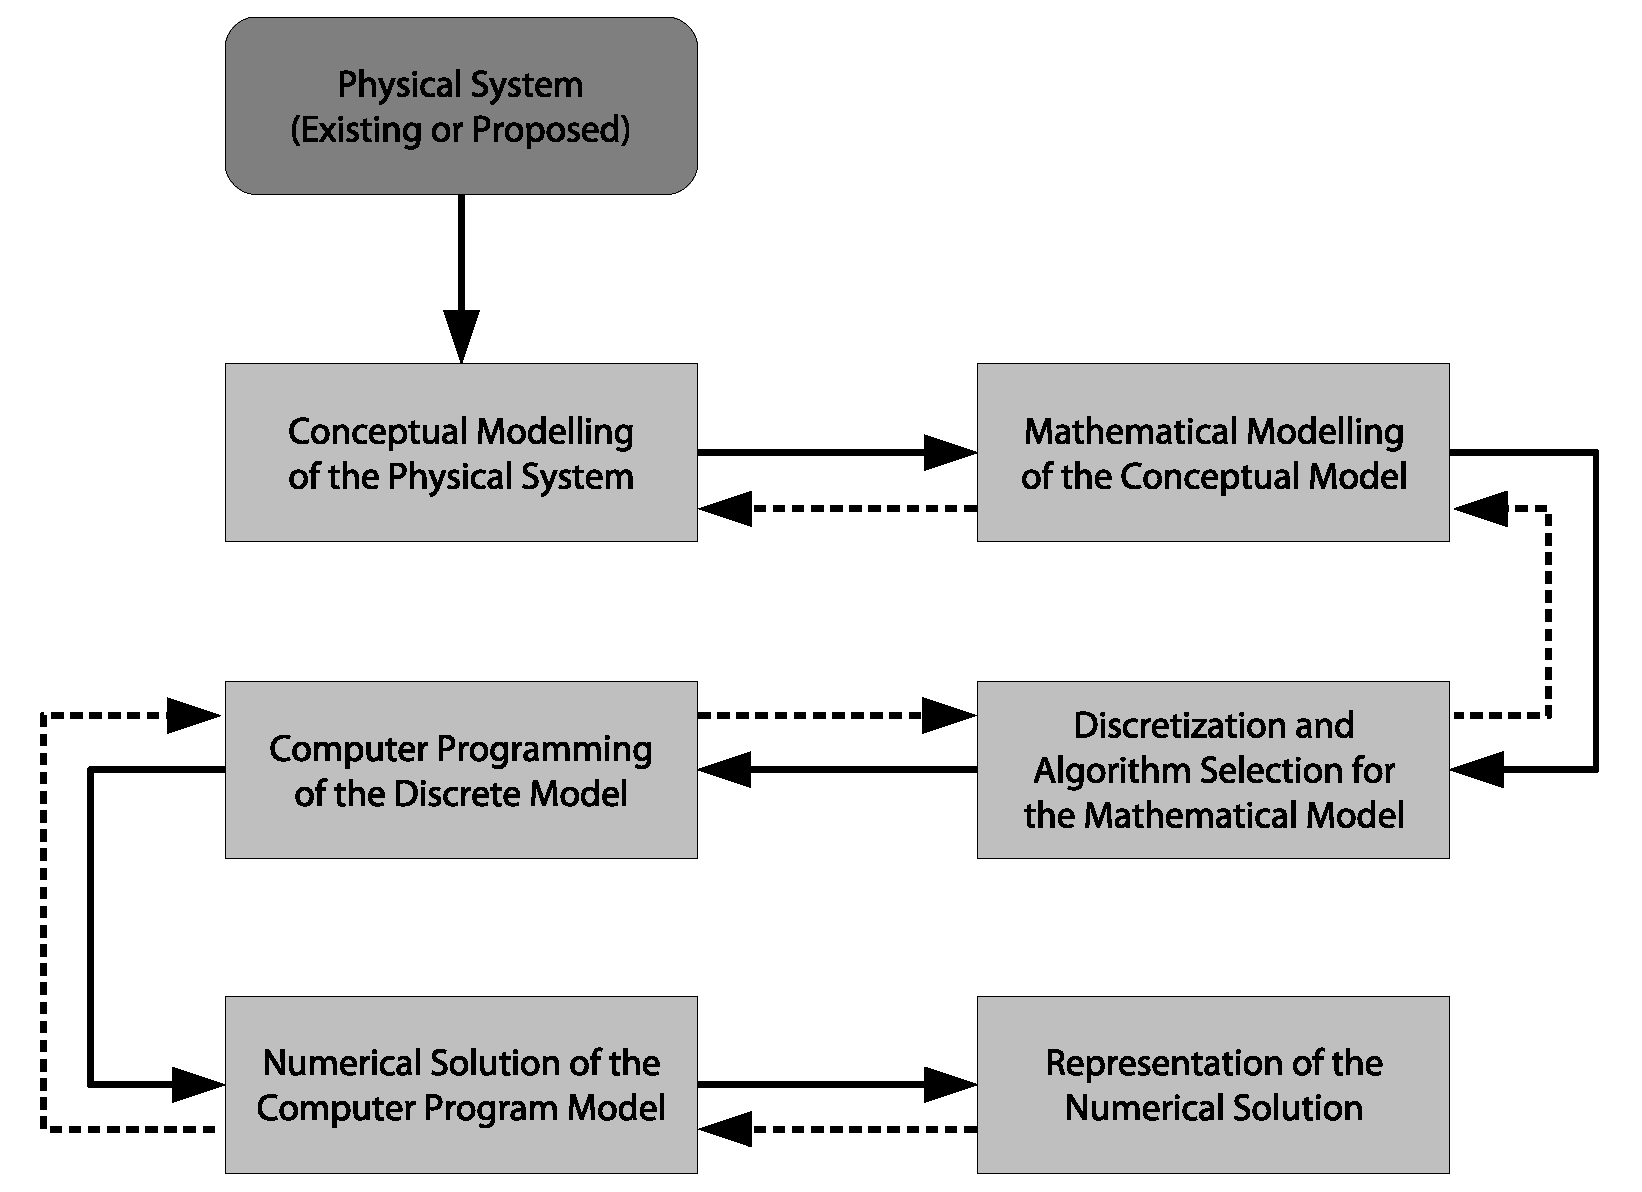
\includegraphics[width=0.90\textwidth]{./img/modelling_phases}
\caption[Proposed phases for computational modelling and simulation.]{Proposed
phases for computational modelling and simulation.
\citep[From][]{oberkampf2002-333}}
  \label{fig:modelling_phases}
\end{figure}

This framework is a synthesis of the reviewed literature, with three substantial
additions compared to a more conventional viewpoint. First, it makes a more
precise distinction between the system and the environment. Second, it places
more emphasis on the distinction between aleatory and epistemic uncertainty in
the analysis. Third, it includes a dominant element in the simulation of complex
physical processes; the numerical solution of non-linear Partial Differential
Equations (PDFs).

\paragraph{Conceptual modelling of of the physical system}
Conceptual issues are considered determining all possible factors.

\paragraph{Mathematical modelling of the conceptual model}
The primary activity of this phase is to develop detailed and precise
mathematical models. The complexity of the models depends on the physical
complexity of each phenomenon being considered, the number of physical phenomena
considered, and the level of coupling of difficult types of physics. Emphasis on
comprehensiveness in the mathematical model should not be interpreted as an
emphasis on complexity of the model. The predictive power of a model depends on
its ability to correctly identify the dominant controlling factors and their
influences, not upon its completeness or complexity. A model of limited, but
known, applicability is often more useful than a more complete model. Any
mathematical model, regardless of its physical level of detail, is by definition
a simplification of reality.

\paragraph{Discretization and algorithm selection for the mathematical
model}
Converting the mathematical models into a form that can be addressed through
computational analysis. Conversion of the continuum mathematics form of the
mathematical model into a discrete, or numerical, model. Specifying the
methodology that dictates which computer runs will be performed in a later phase
of the analysis to accommodate the non-deterministic aspects of the problem.

\paragraph{Computer programming of the discrete model---modular approach}
Algorithms and solution procedures defined in the previous phase are converted
into a computer code.

\paragraph{Numerical solution of the computer program model}
The individual numerical solutions are actually computed.

\paragraph{Representation of the numerical solution}
The representation and interpretation of both the individual and collective
computational solutions. Basically this phase concerns how to present results
for a group of specific audiences.

The erosion models used in the present research are reviewed in the next
section. However, an additional model, the Universal Soil Loss Equation (USLE),
is first discussed since this model embodies the basic concepts underpinning
many more recent models.

\subsection{Universal Soil Loss Equation (USLE)}
\label{sec:UniversalSoilLossEquationUSLE}

The first attempt to develop a soil loss equation for hillslopes was that of
\citet{zingg1940-59}, who related erosion to slope steepness and slope length.
Further developments led to the addition of a climatic factor based on the
maximum 30-minute rainfall total with a 2-year return period
\citep{musgrave1947-133}, a crop factor to take account of the
protection-effectiveness of different crops, a conservation factor and a soil
erodibility factor, consecutively. All these factors were then incorporated
together, modified and up-dated to the Universal Soil Loss Equation (USLE)
\citep{wischmeier1978-537}.

The USLE consists of six factors, which are simply multiplied together to
estimate soil loss although there is substantial interdependence between the
variables \citep{wischmeier1978-537}:
\begin{equation}
\label{eq:usle}
  A = R \times K \times LS \times C \times P
\end{equation}
where $A$ (tonnes$\cdot$ha$^{-1}$ yr$^{-1}$) is average annual soil loss, $R$
(MJ$\cdot$mm$\cdot$hr$^{-1}$ ha$^{-1}$ yr$^{-1}$) is rainfall erosivity, $K$
(t$\cdot$hr$\cdot$MJ$^{-1}$ mm$^{-1}$) is soil erodibility, $L$ (dimensionless
ratio) is the slope-length factor, $S$ (dimensionless ratio) is the
slope-steepness factor, $C$ (dimensionless ratio) is the cropping factor, and
$P$ (dimensionless ratio) is the conservation practice factor.

%
The rainfall erosivity factor ($R$) is related to the raindrop impact effect.
$R$ factor provides relative information on the amount and rate of runoff
associated with the rain. The soil erodibility factor ($K$) is used to represent
the differences of natural resistances of soils to erosion. The slope length
($L$) and steepness($S$) factors provide the topographic information that can
affect the rate of energy dissipation. The cropping factor ($C$) is the ratio of
soil loss from cropped field under specific conditions to the corresponding loss
from tilled, continuous fallow conditions. The conservation practice factor
($P$) is the ratio of soil loss with a specific conservation practice to the
corresponding loss with conventional slope tillage.
%

The USLE uses the empirical results of erosion studies conducted at many
locations over nearly a half-century of research, including rainfall erosivity,
soil erodibility, slope length, slope steepness, cropping and management
techniques, and supporting conservation practices of more than 10,000 plot-years
of data from about 50 locations in 24 states in the US
\citep{wischmeier1978-537}. The results were statistically analysed and the
relationships between the factors incorporated into equation \ref{eq:usle}.

Both the strength and weakness of the USLE lie in its estimation of erosion as
the product of a series of terms for rainfall, slope gradient, slope length,
soil, and cropping factors. However, it does not account for any non-linear
interactions between the factors \citep{wischmeier1978-537,meyer1984-99}.

\citet{nicks1998-377} suggests that USLE may be used to estimate soil loss on a
storm by storm basis where incremental rainfall is available. Rainfall erosivity
index ($EI$) for a rainfall event is calculated by
\begin{equation}
\label{eq:usleerosivityindex}
  EI=R_{0.5} \sum(210+89\,log_{10} I)
\end{equation}
where $I$ is the incremental rainfall intensity and $R_{0.5}$ is the maximum
storm 30 minutes rainfall.
Individual storm erosion amounts may then be calculated with the USLE using this
$EI$ value to replace the $R$ factor in equation \ref{eq:usle}, summed to give a
yearly soil loss, and then averaged to produce a mean annual erosion estimate.

In contrast, \citet{kinnell2005-851} points out important problems of predicting
event erosion using the USLE. One of the main problem described is that, in the
USLE, there is no direct consideration of runoff even though erosion depends on
sediment being discharged with flow, which varies with runoff and sediment
concentration. \citet{kinnell2005-851} concludes that the failure to consider
runoff as a primary factor in the USLE is the factor that causing the USLE to
produce the erroneous prediction of event erosion, which in turn leads to
systematic errors in predicting average annual soil loss.

Since the introduction of the USLE to estimate soil loss, it has become the
conservationists' primary tool for planning purposes
\citep{diaz1987-189,centeri2002-211}. The USLE provides an ease of use and
relatively reliable results, and requires only readily obtainable information in
order to estimate average annual soil loss. However,
\citet{wischmeier1976-misuse} warned about the problem of the misuse of the
USLE.

The database for the original USLE is restricted to the US east of the Rocky
Mountains \citep{wischmeier1978-537}. The base is further restricted to slope
where cultivation is permissible, normally 0 to 7\textdegree, and to soils with
a low content of montmorillonite; it is also deficient in information on the
erodibility of sandy soils \citep{wischmeier1978-537}. It is important to note
that, because the USLE was designed to estimate average annual soil loss from
any specific field over an extended period, soil loss estimates for a specific
year may substantially differ from the long-term average predicted by the
equation \citep{wischmeier1976-misuse}. Extrapolating the relationship beyond
the database for the original USLE, therefore, should be conducted with care.

The basic concepts of the USLE were subsequently used and developed by some
continuous simulation models. Some of these models are CREAMS (Chemicals,
Runoff, Erosion, and Agricultural Management Systems) \citep{knisel1980-creams},
EPIC (Erosion-Productivity Impact Calculator) \citep{williams1984-129}, SWRRB
(Simulator for Water Resources in Rural Basins) \citep{williams1985-970}, WEPP
(Water Erosion Prediction Project) \citep{nearing1989-1587, flanagan1995-usda}.

\subsection{Water Erosion Prediction Project (WEPP)}
\label{sec:WaterErosionPredictionProjectWEPP}

WEPP (Water Erosion Prediction Project) is a process-based model that describes
the processes, such as infiltration and runoff, soil detachment, transport,
deposition, plant growth, senescence, and residue decomposition, that lead to
erosion \citep{flanagan1995-usda}. The model takes four input files, climate,
soil characteristic, slope, and crop management.

WEPP was developed by the USDA-ARS (United States Department of
Agriculture-Agricultural Research Service) as a new-generation water erosion
prediction technology for the routine assessment of soil erosion for soil and
water conservation and environmental planning and assessment
\citep{flanagan2007-1603}. The development of WEPP was initialized with an
intention to replace the `long-used' USLE (See Section
\ref{sec:UniversalSoilLossEquationUSLE}) \citep{nearing1989-1587,
flanagan1995-usda}. WEPP no longer relies on factor values from the USLE,
instead uses separate erodibility parameters for interrill ($K_i$) and rill
erosion ($K_r$) \citep{flanagan1995-usda}. In WEPP, rills are assumed to have a
uniform rectangular cross-section with a uniform spacing of 1 metre. All rills
are assumed to be equally hydrologically efficient \citep{flanagan1995-usda}.

The steady state erosion component of WEPP is based on:
\begin{equation}
\label{eq:weppsedimentload}
  \frac{dG}{dx} = D_f+D_i
\end{equation}
where $G$ represents sediment load, $x$ is the distant downslope, $D_f$ is the
rill erosion rate, and $D_i$ is the interrill erosion rate. $D_f$ and $D_i$ are
calculated on a per rill area basis. Rill erosion, $D_f$, is positive for
detachment and negative for deposition, and calculated by:
\begin{equation}
\label{eq:wepprillerosionrate}
  D_f=D_c(1-\frac{G}{T_c})
\end{equation}
where $T_c$ is the transport capacity of flow in the rill, and $D_c$ is
detachment capacity of the rill flow and:
\begin{equation}
\label{eq:weppdetachmentcapacity}
  D_c=K_r(\tau_f-\tau_c)
\end{equation}
where $K_r$ is rill erodibility parameter, $\tau_f$ is flow shear stress acting
on soil particles, and $\tau_c$ is the critical shear stress or rill detachment
threshold parameter of the soil.
Interrill erosion is given by:
\begin{equation}
\label{eq:weppinterrillerosionrate}
  D_i=K_i I_e \sigma_{ir} SDR_{RR} F_{\textrm{\scriptsize nozzle}}
\frac{R_s}{\omega}
\end{equation}
where $K_i$ is the interrill erodibility, $I_e$ is the effective rainfall
intensity, $\sigma_{ir}$ is the interrill runoff rate, $SDR_{RR}$ is the
sediment delivery ratio, $F_{\textrm{\scriptsize nozzle}}$ is an adjustment
factor to account for sprinkler irrigation nozzle impact energy variation, $R_s$
is the rill spacing, and $\omega$ is the width. Interrill erosion is also
expressed with baseline interrill erodibility as \citep{nicks1998-377}:
\begin{equation}
\label{eq:weppinterrillerosionratealternative}
  D_i=K_{ib} I_e^2 C_C C_G \frac{R_s}{\omega}
\end{equation}
where $K_{ib}$ is baseline interrill erodibility, $C_C$ is the effect of canopy
cover on interrill erosion, and $C_G$ is the effect of ground cover on interrill
erosion. The hydrologic variables that drive the WEPP are the effective rainfall
intensity and duration, the peak runoff rate, and the effective runoff duration.

The USLE erosion database could not be used directly for the WEPP
parametrisation. Three field experiments on cropland, rangeland and forestland
were conducted to determine parameters for $K_r$ and $K_{ib}$ given in equations
\ref{eq:weppinterrillerosionrate} and
\ref{eq:weppinterrillerosionratealternative}. A total of 77 sets of plot data
were collected \citep{nicks1998-377}. Fixed rainfall intensity was applied to
the plots using a rainfall simulator. A comprehensive model description is
available in \citet{flanagan1995-usda}.

Rainfall is represented in the WEPP with the double exponential function. A
storm is described with four parameters, storm amount, average intensity, ratio
of peak intensity to average intensity, and time to peak intensity. A stochastic
weather generator, CLIGEN (CLImate GENerator; \citealp{nicks1995-2}) is used to
generate these storm precipitation inputs. More about CLIGEN is covered later in
Section \ref{sec:ClimateGeneratorCLIGEN}. WEPP then disaggregates these storm
inputs into a single peak storm intensity pattern (time-rainfall intensity
format) for use by the infiltration and runoff components of the model.
\citep{flanagan1995-usda}.

The WEPP model can be used for hillslope erosion processes (sheet and rill
erosion), as well as simulation of the hydrologic and erosion processes on small
watersheds. The hillslope mode predicts soil erosion from a single hillslope
profile of any length. It can be applied to areas up to about 260 hectares in
size. The watershed mode links hillslope elements of specified widths together
with channel and impoundment elements. WEPP is designed to run on a continuous
simulation but can also be operated for a single storm. A modified version of
the hillslope WEPP has been developed for research purposes
\citep{favis-mortlock1999-329,favis-mortlock1996-529}. This is designed to
account for the effects of atmospheric CO$_2$ concentration changes on plant
growth.

In this research, only hillslope mode of the WEPP (v2004.7) was used for
continuous or single-event simulation, depending on the purpose.

\subsubsection{CLIGEN}
\label{sec:ClimateGeneratorCLIGEN}
CLIGEN is a stochastic weather generator, which generates daily time series
estimates of precipitation, temperature, dew point, wind, and solar radiation
for a single geographical point, based on average monthly measurements for the
period of climatic record \citep{nicks1995-2}. The estimates for each parameter
are generated independently of the others \citep{nicks1995-2}.

In comparison to other climate generators, CLIGEN is better at preserving the
low-order statistics of rainfall, temperature, and solar radiation on a daily,
monthly, and annual basis \citep{nicks1995-2}. Unique to CLIGEN is the capacity
to simulate the three additional weather variables to characterize the storm
pattern, namely storm duration, time to peak, and peak intensity, which are
specifically developed for the WEPP simulation \citep{flanagan1995-usda}.

CLIGEN stochastically generates four precipitation-related variables for each
wet day, which are precipitation amount  (mm), $R$, storm duration (hour), $D$,
time to peak as a fraction of the storm duration, $t_p$, and the ratio of peak
intensity over average intensity, $i_p$. Average intensity is defined as $R/D$.
Although it is possible to calculate individual variables manually for each
rainfall event, it is a labour intensive task to calculate the variables for
multiple events.

CLIGEN requires observed precipitation statistics in order to generate these
four precipitation-related variables (Table
\ref{tab:PrecipitaionParametersRequiredByCLIGEN}).

\begin{table}[htbp]
  \centering
  \caption[Precipitation parameters required by CLIGEN]{Precipitation
parameters required by CLIGEN to generate WEPP precipitation inputs (from
personal communication with Bofu Yu, 2003)}
  \label{tab:PrecipitaionParametersRequiredByCLIGEN}
  \footnotesize
    \begin{tabular}{ll}
    \toprule
    \textbf{Parameter} & \textbf{Description} \\
    \midrule
    meanP & Average precipitation (inches) on wet days for each
month\\
    sdP & Standard deviation of daily precipitation (inches) for
each month\\
    skP & Coefficient of skewness of daily precipitation (inches)
for each month\\
    P(W/W) & Probability of a wet day following a wet day for each
month\\
    P(W/D) & Probability of a wet day following a dry day for each
month\\
    {MX.5P} & Average maximum 30-min peak intensity (in/hr) for each
month\\
    TimePk & Cumulative distribution of time to peak as a fraction
of the storm duration\\
    \bottomrule
    \end{tabular}
\end{table}

Precipitation data required to derive the CLIGEN input parameters in Table
\ref{tab:PrecipitaionParametersRequiredByCLIGEN} are time series of daily
precipitation data and sub-daily precipitation data with a time intervals no
greater than 30 minutes (personal communication with Bofu Yu, 2003). In
principle, there is no need to distinguish these two types of precipitation data
because sub-daily data can be accumulated to produce daily values. In practice,
however, these two types of data usually come from two different sources. The
coverage of the daily data, both in space and time, is much more extensive in
comparison to sub-daily data at short time intervals. In addition, the two types
of data are normally stored in different formats. It is therefore useful to
treat the two types of precipitation data separately.

CLIGEN (version 4.2) was previously released with WEPP version 2001.3. However,
this version of CLIGEN had a major coding error and was modified substantially
\citep{yu2000-301}. CLIGEN (version 4.2) computed a ratio $\omega = R_{0.5}/R$,
where both $R_{0.5}$ and $R$ were rainfall depth (originally in inches).
$R_{0.5}$ had been converted from inches into millimetres (mm), while $R$ was
not \citep{yu2000-301}. The CLIGEN code was thus changed to correct this error.
This however led to extensively increased storm durations.

To accommodate the correction of unit conversion error, it was necessary to
incorporate two important modifications in the CLIGEN codes. First, a new
algorithm to determine the monthly means of the maximum 30-min rainfall depth
was implemented. Secondly, the parameter values for storm duration and the
coefficient of variation for the ratio of the maximum 30-min rainfall depth to
daily rainfall required in CLIGEN were estimated using the break-point rainfall
data \citep{yu2000-301}.

This error in the CLIGEN code has certainly affected the results from the
earlier studies, which employed the previous versions of WEPP and CLIGEN to
estimate soil loss
\citep{truman1993-405,zhang1995-1069,zhang1995-1079,zhang1996-855,
baffaut1996-447,laflen1997-96,baffaut1998-756,favis-mortlock1999-329}.

The version of CLIGEN at the time of writing is version
5.22564\footnote{http://horizon.nserl.purdue.edu/Cligen/, April 2006}. This is
the version used in this research.


\subsection{European Soil Erosion Model (EUROSEM)}
\label{sec:EuropeanSoilErosionModelEUROSEM}

EUROSEM is a dynamic distributed event-based model for simulating erosion,
transport and deposition of sediment over the land surface by interrill and rill
processes \citep{morgan1998-389}. The model has explicit simulation of interrill
and rill flow; plant cover effects on interception and rainfall energy; rock
fragment effects on infiltration, flow velocity and splash erosion; and changes
in the shape and size of rill channels as a result of erosion and deposition
\citep{morgan1998-389}. It can be applied to a small field and up to a small
catchment.

EUROSEM requires a one-minute resolution breakpoint rainfall data for the storm.
The model then computes, using the breakpoint rainfall data, the interception of
the rain by the plant cover, the generation of runoff as infiltration excess,
soil detachment by raindrop impact, soil detachment by runoff, transport
capacity of the runoff and deposition of sediment. The model has a modular
structure that aims to make further improvements of the model easier. The model
considers the followings:
\begin{itemize}
\item the interception of rainfall by the plant cover
\item the volume and kinetic energy of the rainfall reaching the ground surface
as direct throughfall and leaf drainage
\item the volume of stemflow
\item the volume of surface depression storage
\item the detachment of soil particles by raindrop impact and by runoff
\item sediment deposition
\item the transport capacity of the runoff
\item frozen soils and stoniness
\end{itemize}

The flow chart for EUROSEM is shown in Figure \ref{fig:eurosem_flow_chart}.

\begin{figure}[htbp]
  \centering
    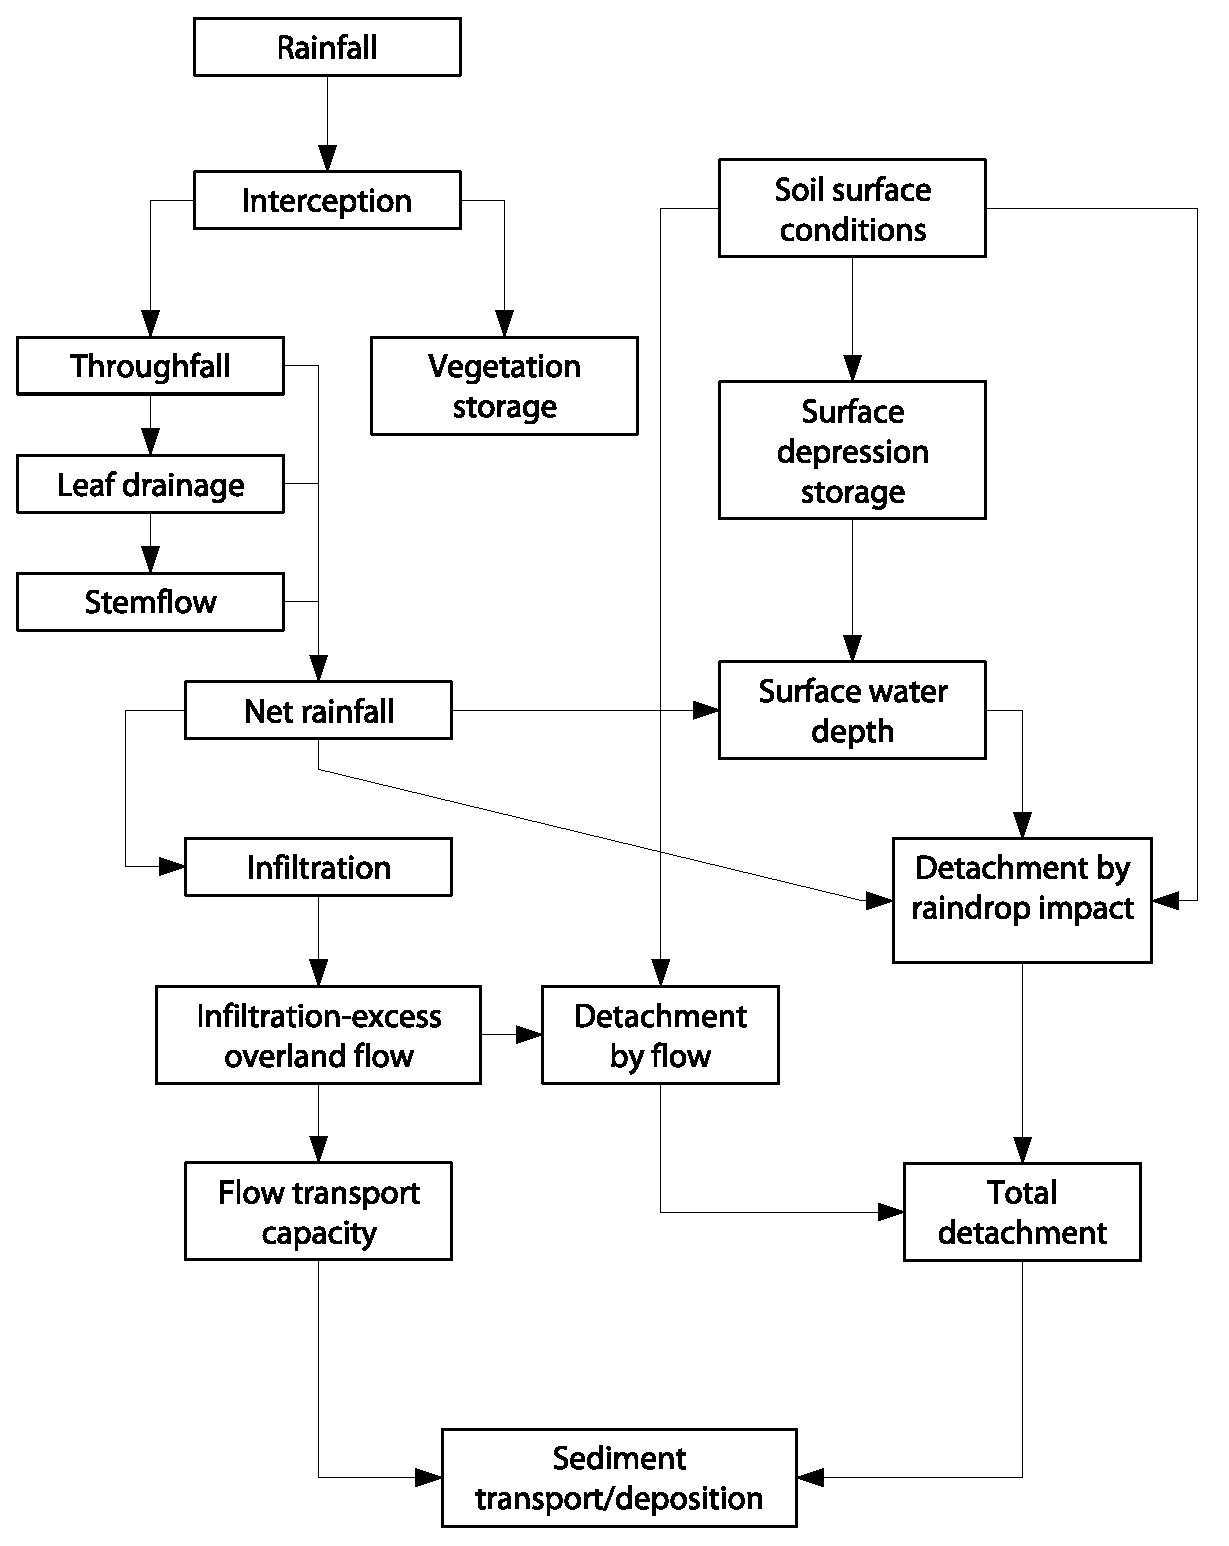
\includegraphics[width=0.80\textwidth]{./img/eurosem_flow_chart}
  \caption[Flow chart of EUROSEM]{Flow chart of EUROSEM (from
\citealp{morgan1998-389})}
  \label{fig:eurosem_flow_chart}
\end{figure}

Runoff generator and the water and sediment routing routines of EUROSEM are from
another model called KINEROS \citep{woolhiser1990-kineros}. The volume of
sediment passing a given point on the land surface at a given time is calculated
by a mass balance equation:
\begin{equation}
\label{eq:eurosemmassbalance}
  \frac{\partial(AC)}{\partial t}+\frac{\partial(QC)}{\partial x}-e(x,t)=
q_s(x,t)
\end{equation}
where $C$ is sediment concentration (m$^3$/m$^3$), $A$ is the cross sectional
area of the flow (m$^2$), $Q$ is the discharge (m$^3$/s), $q_s$ is external
input or extraction of sediment per unit length of flow (m$^3$ s$^{-1}$
m$^{-1}$), $e$ is net detachment rate or rate of erosion of the bed per unit
length of flow (m$^3$ s$^{-1}$ m$^{-1}$), $x$ is horizontal distance (m), and
$t$ is time (s).
The net detachment rate, $e$, is given as:
\begin{equation}
\label{eq:eurosemnetdetachmentrate}
  e = DR + DF
\end{equation}
where $DR$ is the rate of soil particle detachment by raindrop impact (m$^3$
s$^{-1}$ m$^{-1}$), and $DF$ is the balance between the rate of soil particle
detachment by the flow and the particle deposition rate (m$^3$ s$^{-1}$
m$^{-1}$).

The EUROSEM simulates erosion and deposition by calculating three main
processes, soil particle detachment by raindrop impact, soil particle detachment
by runoff, and transport capacity of the flow.

\paragraph{Soil particle detachment by raindrop impact}
\label{sec:SoilParticleDetachmentByRaindropImpact}
Soil detachment by raindrop impact ($DR$) for time step ($t_s$) is expressed as
a function of the kinetic energy of the rainfall at the ground surface, the
detachability of the soil and the surface water depth:
\begin{equation}
\label{eq:EUROSEMsoildetachmentbyraindropimpact}
  DR = \frac{k}{\rho_s} {KE} e^{-zh}
\end{equation}
where $k$ is an index of the detachability of the soil (m$^3$/J), $\rho_s$ is
the sediment particle density (=2.65 Mg/m$^3$), $KE$ is the total kinetic energy
of the net rainfall at the ground surface (J/m$^2$), $z$ is an exponent taken as
equal to 2.0 which varies between 0.9 and 3.1 \citep{torri1987-149}, and $h$ is
the mean depth of the surface water layer (m).
The kinetic energy of the rainfall is the combined energy from direct
throughfall and leaf drainage. The energy of the direct throughfall is computed
using raindrop size distribution found by \citet{marshall1948-165}. The energy
of the leaf drainage is based on a study by \citet{brandt1990-687}.

\paragraph{Soil particle detachment by runoff}
\label{sec:SoilParticleDetachmentByRunoff}
Soil particle detachment by runoff is based on a theory proposed by
\citet{smith1995-517}, and is given as:
\begin{equation}
\label{eq:eurosemsoilparticledetachmentbyrunoff}
  DF = \beta w v_s (TC-C)
\end{equation}
where $DF$ is the rate of detachment of soil particles by the flow, $\beta$ is a
flow detachment efficiency coefficient ($\beta=1$ when deposition is taking
place and $\beta < 1$ for cohesive soils when $DF$ is positive), $w$ is the
width of the flow (m), $v_s$ is the setting velocity of the particles in the
flow (m/s), $TC$ is the sediment concentration in the flow at transport
capacity, and $C$ is the actual sediment concentration in the flow.

\paragraph{Transport capacity of flow}
\label{sec:TransportCapacityOfTheFlow}
EUROSEM uses two separate transport capacity relationships for rill and
interrill flows. Rill and interrill transport capacities are based on
\citet{govers1990-45} and \citet{everaert1991-513}, respectively. The equation
for rill transport capacity ($TC_{r}$) is expressed as:
\begin{equation}
\label{eq:EUROSEMRillTransportCapacity}
  TC_{r} = c(\omega - \omega_c)^{\eta}
\end{equation}
where $\omega$ is unit stream power (cm/s) which is defined as $\omega = 10
\upsilon s$ ($\upsilon$ = mean flow velocity (m/s) and $s$ = slope (\%)),
$\omega_c$ is a critical value of unit stream power (0.4 cm/s), and $c$ and
$\eta$ are experimentally derived coefficients related to the median particle
size of the soil.
Interrill transport capacity ($TC_{ir}$) is modelled as:
\begin{equation}
\label{eq:EUROSEMInterrillTransportCapacity}
  TC_{ir} = \frac{b}{\rho_s q}\left[(\Omega -
\Omega_c)^{\frac{0.7}{n}}-1\right]^{\kappa}
\end{equation}
where $b$ is a function of particle size, $\rho_s$ is the sediment density
(Kg/m$^3$), $\Omega$ is Bagnold's modified stream power, $\Omega_c$ is a
critical value of Bagnold's modified stream power, $n$ is Manning's $n$, and
$\kappa$ = 5. Sediment delivery to the rills is simulated depending on the
transport capacity of the interrill flow.

Since EUROSEM uses a dynamic rather than steady-state approach used by WEPP, it
gives a better understanding of the spatial and temporal distribution of runoff
and erosion. However, the result of the model simulation may become considerably
uncertain due to its process-based nature that requires detailed model
parametrization \citep{quinton1998-65}. Particularly, EUROSEM requires high
resolution rainfall data (ideally, 1-min breakpoint data), soil hydrological
information, detailed surface geometry, and soil mechanical and vegetation
characteristics. Because of the detailed requirements of the model, application
of the model is greatly restricted to where such data are available.

\citet{parsons2000-181} found that because EUROSEM ignores small-scale
heterogeneities in the infiltration characteristics of soil, the model generates
delayed initiation times for runoff, so that predicted hydrographs showed the
commencement of runoff later than observed. Such variabilities in the
infiltration characteristics may be responsible for the comparatively rapid
initiation of runoff on the plot. They also found that the subsequent soil
detachment by runoff in interrill areas is overestimated by the model even
though, according to the model document, detachment by flow should be negligible
in interrill areas.

After personal communication (16 Jun 2004) with Anthony J. Parsons , it is noted
that EUROSEM may have a unit conversion error. The model document states that
the flow depth ($h$) in equation \ref{eq:eurosemsoilparticledetachmentbyrunoff}
is in metres. However, a study by \citet{torri1987-149} on which this equation
is based indicates that the height is in millimetres (see Figure 2 in
\citet{torri1987-149}). Anthony J. Parsons suggests that the height is in
centimetres rather than either metres or millimetres. If confirmed, this error
would have major effects on EUROSEM's ability to estimate runoff and erosion.

%First does the storm pattern affect the  runoff coefficient (same amount of
%rain but different amount of runoff) so  do differences in erosion result
%simply from more or less runoff?
%Secondly,  does the intensity pattern affect detachment so you get more or
%less erosion  because of the detachment effect.  We have something to say
%about that (sort of) in a paper in ESPL that should appear at some point
%(when I submit it!).
%So I think Mintae needs to look carefully at what is happening in the 2
%models in terms or runoff coefficients and detachment rates.

The version of EUROSEM used in this research is 3.9 (14/12/1998), which is the
current version of the model. It seems that the model development has been
ceased for some time.
%It may have been the case that the model developer have abandoned the model.

\subsection{RillGrow}
\label{sec:ModelDescriptionRillGrow}

While the later two erosion models (i.e. WEPP and EUROSEM) reviewed previously
are capable of realistically simulating rates of soil erosion, they (in common
with all other present-day erosion models) have a number of conceptual
shortcomings. For example, rills are considered to be equally spaced, with
regular cross-sections, and to be of similar hydrological efficiency. In
reality, rills are not necessarily spaced regularly and often have irregular
cross-sections. Adjacent rills may also vary greatly in their ability to
transport runoff and sediment \citep{favis-mortlock1996-248}. Additionally,
while such models separately describe the different processes responsible for
erosion in rill and interrill areas, they largely fail to acknowledge the
physical link that exists between the processes operating in the two zones
\citep{favis-mortlock2000-2173}.

The development of the RillGrow model
\citep{favis-mortlock1996-248,favis-mortlock1998-353,favis-mortlock2000-2173,
favis-mortlock2003-127,favis-mortlock2004-349} started with a consideration of
these shortcomings, and a question `\emph{Is the initiation and development of
hillslope rill systems driven by relatively simple rules acting on a much
smaller scale?}'. To test this hypothesis, a self-organising dynamic systems
approach was used to simulate the initiation and development of a rill network
on the bare soil of a small (e.g.\ plot-sized) hillslope area.

RillGrow is a single-event model, which generates realistic rill networks by
simulating, on a grid of microtopographic elevations, the combined erosive
action of overland flow moving between the cells of the grid. Surface water
arrives, a single raindrop at a time, on random cells of the grid. Runoff moves
over the grid following the steepest microtopographic gradient; as it moves, it
erodes the soil surface by lowering the elevation of the soil's surface. Each
change in elevation affects the routing of subsequent runoff: the result is a
feedback loop in which flow patterns over the grid at any time depend on earlier
flow patterns (and hence erosion), these flow patterns then condition subsequent
flow patterns, and so on (Figure \ref{fig:rillgrow_feedback_concept}).

\begin{figure}[htbp]
  \centering
    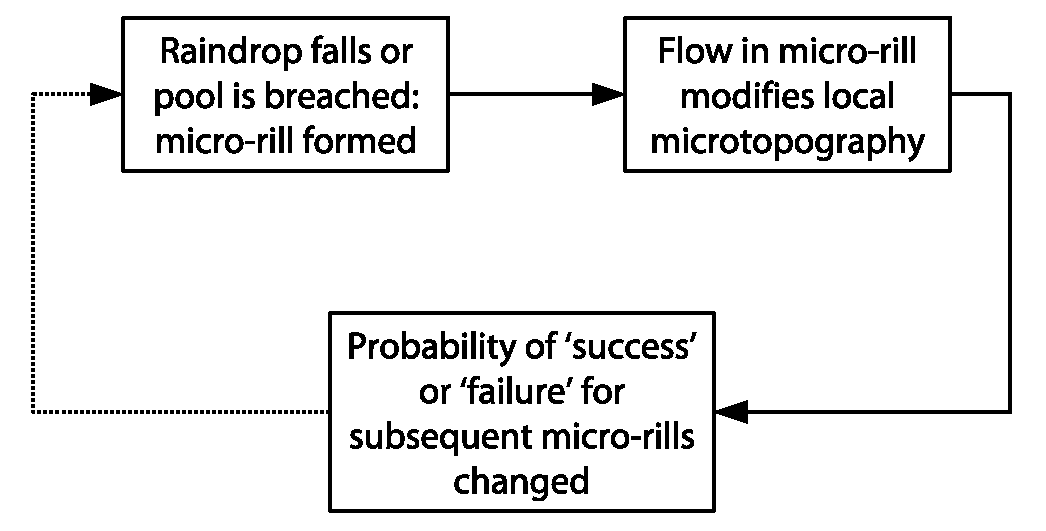
\includegraphics[width=0.80\textwidth]
{./img/rillgrow_feedback_concept}
  \caption[The conceptual feedback loop of RillGrow]{The conceptual
feedback loop of RillGrow \citep[From][]{favis-mortlock1998-353}}
  \label{fig:rillgrow_feedback_concept}
\end{figure}

The first version of the RillGrow model was able to realistically simulate rill
initiation and development, reproducing several features of observed rill
systems \citep{favis-mortlock1996-248,favis-mortlock1998-353}:
\begin{enumerate*}
  \item a narrowing of rill spacing with increased slope angle
  \item an increased contribution of rill erosion with downslope distance
  \item a non-linear increase of total erosion with slope steepness
  \item an increase in rill depth below confluences and micro-rill piracy
\end{enumerate*}

However, RillGrow 1 has some important limitations. It ignores important process
descriptions (e.g.\ infiltration, deposition), and the hydraulics of rill
initiation are oversimplified. It also does not operate in a true time domain,
since at any moment during the simulation, only a single `packet' of overland
flow is moving over the topographic grid. Infiltration is ignored, thus all
water on the grid is assumed to be rainfall excess, and transport capacity is
assumed to be infinite because no deposition can occur
\citep{favis-mortlock2000-2173}.
All these limitations meant that it was not possible to validate the model in a
deterministic way, e.g. by comparing simulated and laboratory-produced rill
networks.

A second version of the model (`RillGrow 2') was developed to overcome some of
these limitations, and allow more rigorous validation
\citep{favis-mortlock2000-2173}. In RillGrow 2, overland flow in effect moves
concurrently between cells of the
microtopographic grid. Such concurrency is not easy to achieve on a
serial-processing computer, since only one instruction can be carried out at a
time. Concurrent processing is simulated in RillGrow 2 in the following way:
during a given timestep, outflow from each `eligible' wet cell is routed in a
random sequence which differs for each timestep. This variation in sequence is
necessary to prevent any artefacts of flow pattern which might result from a
fixed routing sequence. Over a sufficient number of timesteps, the model in
effect operates in `parallel', i.e. concurrently, in a true time domain.

\begin{table}[htb]
  \centering
  \small
  \caption[The main routing algorithm used in RillGrow 2]{The main routing
algorithm used in RillGrow 2 \citep[From][]{favis-mortlock2000-2173}. Note that,
while
this set of rules does not change during the model simulation, the result of
applying the rules to a given cell depends on the past history of elevation
change both for that cell, and for adjacent ones.}
  \label{tab:TheMainRoutingAlgorithmUsedInRillGrow2}
    \begin{tabular}{p{0.9\textwidth}}
    \toprule
For each iteration:\\
\\
Drop raindrops on random cells on the spatial grid. Each drop makes (or adds to,
if the cell is already `wet') a store of surface water for that cell.\\
\\
Go through all `wet' cells in a random sequence (which is different each
iteration). For each `wet' cell, check whether sufficient time has elapsed for
flow to have traversed the cell. If it has, then do the following:\\
\begin{itemize}
  \item Find the adjacent cell which has the steepest downhill (i.e.\
outflow) energy gradient. Note that this adjacent cell may or may not be already
`wet'.
  \item Attempt to level the energy gradient between these cells by
outflow of an appropriate volume, adding to (or creating) the store of surface
water on the adjacent cell.
  \item Erode this cell (i.e.\ lower its soil-surface elevation) by an
amount which depends on the outflow volume and velocity.
  \item If there are other adjacent cells with downhill energy gradients,
process these as above.
\end{itemize}\\
%\addlinespace[-2mm]
    \bottomrule
    \end{tabular}
\end{table}

RillGrow 2 also uses a refined set of basic rules for the routing algorithm
(Table \ref{tab:TheMainRoutingAlgorithmUsedInRillGrow2}). A probabilistic
expression by \citet{nearing1991-81}, based on the random occurrence of
turbulent bursts, is used to represent flow detachment. Sediment load is
compared with transport capacity, which is calculated using stream power in an
s-curve expression developed by \citet{nearing1997-865}. Deposition is estimated
using the approach of  \citet{lei1998-3157}: this assumes deposition to be a
linear function of the difference between sediment load and transport capacity.

Infiltration is now simulated by RillGrow 2, however the approach used is still
very simple (Favis-Mortlock, personal communication 2006). Splash redistribution
is also represented, using the diffusion-based approach of
\citet{planchon2000-131}, modified to include attenuation due to surface water
depth (Favis-Mortlock, personal communication 2006). Additionally, a simple
linkage is made between overall volumes of sediment detached or deposited by
splash in any timestep, and volumes of sediment currently being transported by
overland flow (Favis-Mortlock, personal communication 2006). The distribution of
raindrop volumes is assumed to be normally distributed (Favis-Mortlock, personal
communication 2006).

In comparison to models such as WEPP and EUROSEM, RillGrow makes no explicit
separation between rill and interrill areas. Soil erosion amount is calculated
as the result of summation of soil losses from all areas.
%Explicit separation of rill and interrill areas turns out to be unnecessary,
%however.
Flow velocities are so low on interrill areas that little detachment occurs as a
result. On such areas, splash redistribution dominates.

\citet{favis-mortlock2000-2173} observes that RillGrow 2 replicates the
responses of RillGrow 1 including realistic rill spacing with respect to slope
gradient. In addition, the simulated spatial patterns of erosion compare well
with
laboratory-based observations, as do total erosion, variation in rill depth, and
time-series of runoff and soil loss. Braided or dendritic flow patterns can be
made to emerge by varying rainfall intensity. At low rainfall intensities,
however, the definition and stability of rill patterns is less well defined.

As originally constructed, RillGrow 2 assumed each storm to have a constant
rainfall intensity. For the research described in this thesis, RillGrow 2 has
been modified to use breakpoint rainfall data. This allows the model to simulate
rill initiation and development and total soil loss, as affected by rainfall
intensity changes (Favis-Mortlock, personal communication 2006).


%\nolinenumbers
%\linenumbers*
\chapter{RESEARCH BACKGROUND AND OBJECTIVES}
\label{sec:RESEARCHOBJECTIVES}

\section{Background and Direction}
\label{sec:ResearchBackgroundandDirection}

\begin{quotation}
\small ``If politics is the art of the possible, research is surely the art of
the soluble. Both are intensely practical-minded affairs.'' (Peter Medawar
(1915-1987) ``The Act of Creation'' in ``New Statesman'', 19 June 1964)
\end{quotation}

Before going into the aim of this research, it seems more appropriate to explain
the scope and direction of this research first. In this way, readers may
understand more clearly the research aim and rationale behind the approach used
in this study.

When this research was first begun, the initial plan was to use the simulated
future rainfall intensity output from RCM as input to one or more erosion
models, in order to improve upon then-current forecasts of future erosion rates
and eventually to develop a method to link RCM results and erosion models.

However, after a number of pilot simulations with models at an early stage, it
became apparent that RCM rainfall data could not (and still cannot) be used
directly for erosion simulations. In order to use RCM data for the approach
initially proposed, the data should be able to provide rainfall intensity
information on a required scale (i.e.\ sub-hourly) with an acceptable level of
confidence. RCM data do not hold sufficiently detailed (i.e.\ temporally and
spatially) information that can be used for erosion simulations directly, and
were not reliable enough for this type of approach yet---and still they are not
\citep{nearing2001-229,michael2005-155,o'neal2005-165}.

Thus, another route was taken to resolve this issue. In order to obtain rainfall
data usable for erosion modelling in terms of scale and representable as
future rainfall, observed rainfall data were analysed to determine trends of
rainfall intensity. Once rainfall intensity trends are determined, probable
scenarios of future rainfall intensity changes can then be built by applying the
trend onto observed rainfall intensity.
%More on this approach is discussed in Chapter
%\ref{sec:RainfallCharacteristicsOfTheStudyArea}.

Rather later, more problems were identified with selected erosion models, in
that there were aberrant model responses to changes in a certain aspects of
rainfall intensity (See Chapter
\ref{sec:EFFECTSOFCONTINOUSANDDISCONTINUSSTORM}). This implied that there were
deficiencies in the process understanding on which the models are based. Thus,
the original plan had to be put on hold until both, improved erosion models and
more reliable RCM rainfall data, become available.

Accordingly, the focus of the research has evolved into the evaluation of the
response of erosion models to rainfall intensity changes, and implicitly the
process understanding on which the models are based, using arbitrary changes in
rainfall intensity. In turn, this will assist in improving the performance of
erosion models with respect to changes of rainfall intensity by highlighting
where the current problem exists. Consequently, greater knowledge here will,
once future changes in rainfall intensity become better known, improve our
ability to estimate future rates of erosion.
%%
%Favis-Mortlock, D.T., Boardman, J. and MacMillan, V.J.(2001). The limits of
%erosion modeling: why we should proceed with care. In, Harmon, R.S. and Doe
%III, W.W. (eds). Landscape Erosion and Evolution Modeling, Kluwer
%Academic/Plenum Publishing, New York, pp. 477-516.
%%

\section{Objectives and Rationales}
\label{sec:ResearchObjectives}

The main objective of this research is to investigate:
\begin{itemize}
 \item possible implications of climate change for future soil erosion with
reference to rainfall intensity changes by analysing the response of erosion
models to arbitrary rainfall intensity changes, and
 \item implicitly the process understanding on which the models are based.
\end{itemize}
To accomplish these aims, the research was carried out in two parts:
\begin{itemize}
 \item \textit{Rainfall Intensity and Erosion: Model Descriptions and
Responses} and
% \item \textit{ Observed Rainfall Characteristics (and Intensity) of the Study
%Site} and
 \item \textit{Implications for Model-based Studies of Future Climate Change and
Soil Erosion}.
\end{itemize}

%To accomplish this, the research was carried out as three stages:\
%\textsl{Rainfall Intensity and Erosion Modelling}, \textsl{Observed
%Precipitation of the Research Site} and \textsl{Implications for Future Climate
%Change and Erosion}.

In the first part, \textsl{Rainfall Intensity and Erosion: Model Descriptions
and Responses}, three process-based erosion models, WEPP, EUROSEM and RillGrow,
were used to investigate their responses (i.e.\ runoff and soil loss rates) to
various rainfall intensity conditions. The process descriptions of these models
were examined in regard to how they make use of rainfall intensity.

The reason for using multiple models is to minimize the probability of
uncertainty that may increase when relying on a single model
\citep{ipcc2001-881}. The design purposes of erosion models varies from
model to
model, and so do their artefacts \citep{favis-mortlock1998-141,jetten1999-521}.
Thus, it is problematic to use only one model, unless there are some
observational data that it can be compared to, as it is not possible to know to
what extent the result from the model is unique to that model
\citep{favis-mortlock1998-141,jetten1999-521}.

For the same reason, it was suggested that, in the study of future climate
change, one should not rely on a single GCM or RCM. This is also the case for
the downscaling \citep{mearns2003,wilby2004}. In such studies, the same
principle---more is better than one---is always in practice \citep{wilby2004}.
This principle may equally be applied to the study of soil erosion modelling.

It would have been possible to use only two erosion models. However, this may
have led to another problematic situation. For example, if two erosion models
show contrasting results, it will be very difficult to decide which one to
accept and which one to accept not---although it may still be debatable
whether the resulting conclusion is applicable to the reality even when both
models agree. A good answer to this dilemma may be found in an old fisherman's
saying: ``Never go to sea with two chronometers; take one or \emph{three}.''
%****** good, but need to be clearer, since this is important
Therefore, \emph{three} erosion models were used in this study.
% in this thesis:\ WEPP,EUROSEM and RillGrow.

Comparing results from three models, instead of one or two models, may increase
our chances to relate modelling results back to the real world.
% provide less uncertainty than comparing results from one or two models.
If all three models show similar responses---even though the chances of
incurring such result are slim---to rainfall intensity changes, the agreed
results among three models may possibly be related to the real world
\citep{araujo2007-42}.
More importantly, however, when any of the models disagree, further
investigation should follow to look into the model equations, programming
algorithms and codes in order to find out what may have caused such
disagreement. By comparing outputs from these models, we could also identify
their weaknesses and, in turn, improve them for future researches.

A primary purpose of these erosion models (i.e. WEPP, EUROSEM and RillGrow) is
to simulate soil erosion.
Even though each model has its unique way of simulating erosion
processes, the main design purpose is the same; to simulate the real-world
erosion processes. Erosion models are developed in order to:
\begin{itemize*}
  \item Use them as important predictive tools for future or unmonitored
landscapes;
  \item Study how different factors play a role in erosion;
  \item Understand erosion processes; and in turn,
  \item Minimise environmental issues caused by soil erosion.
\end{itemize*}
Because of these purposes, \emph{ideally} all erosion models should be based on
similar understanding of erosion, and simulate erosion similarly. %really???
This general idea was taken into account and it was hypothesised that the
models selected for this research produce similar results when a given
rainfall intensity was applied to them.
Yet, the reality is somewhat different from the ideal, and one may still expect
that the models may produce divergent responses
\citep{favis-mortlock1998-141,jetten1999-521}. However, it is important to
investigate this diversity of model outputs in order to identify and improve
areas where our understanding is limited.
%because of physical difficulties in creating appropriate conditions to study.
%I need to support my argument more here. also, what extent the models are
%different and similar.

\begin{quotation}
\small ``The purpose of models is not to fit the data, but to sharpen the
questions.'' (Samuel Karlin, Eleventh RA Fisher Memorial Lecture, Royal Society,
20 April 1983)
\end{quotation}

The above statement by Karlin highlights one of reasons why many models are used
in numerical and analytical studies. In most cases, a model is based on
knowledge that is limited by what we already know about the process. There can
be a range of different understandings of the same processes---soil erosion
processes in this case. These understandings are expressed as mathematical
equations, and then translated into computing languages, and finally put
together as a model with which our understandings of the processes can be
tested. This provides us with a complete control over affecting parameters.
Generally, it is not possible to gain complete control over affecting factors
with field experiments or with laboratory experiments because modifying only
one factor without altering other factors is not feasible. Using a model, an
individual input parameter may be isolated, adjusted and investigated to find
its effects on the overall erosion process, while keeping all the remaining
parameters constant. Of course, this still does not guarantee a correct
prediction by the model. However, this kind of approach helps to ``sharpen the
questions''. More focused questions from modelling studies may help to fill out,
or rather to pinpoint the gap in our understanding of the processes. There have
been several studies employing this type of approaches already
\citep{favis-mortlock1995-365,favis-mortlock1999-329,pruski2002-7,
nearing2005-131}.

One more reason for using a model can be explained by the duration of
experiments. According to \citet{web_[Se-list]}, in the case of erosion-plot
experiments, the outcome may be very difficult to interpret unless the
experiments were conducted for \emph{a long period of time} because of high
variability in the observational data. The result may not be significant unless
the record is of sufficient length, treatments are greatly different, and a
sufficient number of replicates is employed \citep{nearing1999-1829}.
\citet{web_[Se-list]} stated ``\ldots it needs to be understood that these
estimates [which are estimated using short periods of record] can have great
error and that longer term records are needed to refine these estimates.'' He
then suggested to design plots and collect the data ``in such a way as to be
able to use the data in evaluation of models and development of parameters that
can be used to extrapolate results to the much wider climatic record than one
can experience in a few years''.

Hence, using a model can be a good choice of method over observational
experiments in some cases like above---and may well be the only method when
estimating a long-term effect which cannot be observed. For example, in the
study by \citet{favis-mortlock1997-79}, EPIC (Erosion-Productivity Impact
Calculator) was used to reproduce the past erosion processes on a hillslope in
South Downs, UK from 7000 BP to the present day, in order to find out the major
factors influencing past soil erosion. In a case like this, modelling is clearly
the only possible choice. Modelling is also the only choice for the study on
impacts of future climate or land-use changes on soil erosion
\citep{favis-mortlock1995-365,favis-mortlock1999-329,pruski2002-7,
pruski2002-climate,nearing2005-131}.

Therefore, the first part of this study, using WEPP, EUROSEM and RillGrow, aims
to investigate:
\begin{itemize*}
  \item necessary information for rainfall intensity properties to simulate soil
erosion,
  \item responses of selected models to changes of rainfall intensity
properties,
  \item underlying processes of the models for computing rainfall intensity
properties and
  \item the applicability of the same models in the subsequent research.
\end{itemize*}

%In the second stage, \textsl{Observed Rainfall Characteristics (and Intensity)
%of the Study Site}, a series of observed high-resolution rainfall data were
%obtained to determine a trend of rainfall intensity changes at the research
%site
%in the South Downs, UK (Figure \ref{fig:DailyRainfallDataSite}). One of the
%reasons for choosing this particular site is because the area has been
%extensively monitored for soil erosion since the late 1970s
%\citep{boardman1995-177,boardman2003-176}, so that data availability of the
%site
%is therefore reasonably great. In addition, there is a well-established
%expertise about the area that can be referenced to the current research
%\citep{boardman1995-177,favis-mortlock1995-365,favis-mortlock1997-79,
%favis-mortlock1998-141,boardman2001-346,boardman2003-176}. The datasets used
%here are temporally and spatially different; monthly 0.5\textdegree\ grid data,
%daily station data and tipping-bucket gauge data.
%
%Moreover, as stated previously, this approach was taken because of the
%important
%issues discovered from RCM data. Probable scenarios of future rainfall
%intensity
%were created based on the \textit{present-day} rainfall intensity trend. These
%present trends were also compared with GCM predicted data. The resulting
%scenarios were later used to make predictions regarding future erosion.

%In short, the second stage aims to
%\begin{inparaenum}[1)]
%  \item provide a solution for the problem that have been identified with RCM
%rainfall data during the initial investigation of this research by analysing
%observed rainfall data in the various scales to determine rainfall intensity
%trends;
%  \item build scenarios of future rainfall intensity based on the
%\textit{present-day} rainfall intensity trend, which may, in turn, be used for
%the final stage of the research.
%\end{inparaenum}
%You imply that you are using present-day climate data to predict future
%erosion. No-one can do that! What you are doing, of course, is to create
%scenarios of future rainfall which are *based on* present-day rainfall (and
%then these are used to make predictions re. future erosion). *I* know that you
%know this, but the text isn't clear. Be as clear as possible: it is easy to
%create confusion in the mind of the reader if you are not completely clear.

In the second part, \textsl{Implications for Model-based Studies of Future
Climate Change and Soil Erosion}, future rainfall intensity scenarios
were used to estimate erosion rates using WEPP, one of the soil
erosion models used in this research. WEPP is used in the second part because it
is a continuous simulation model, which is capable of simulating long-term
erosion taking into account the factors such as the complex overlap of
temporally and spatially diverse distributions of rainfall, erodibility, soil
conditions, plant cover \citep{nearing2006-145}.

The second part of this thesis aims to:
\begin{itemize*}
  \item suggest the best possible way of investigating impacts of rainfall
\textit{intensity} changes on future erosion and
  \item try to test out the suggested method with intensity-change scenarios
constructed previously.
\end{itemize*}

% The aims of all the stages are summarised below:
% \begin{enumerate}
%   \item To investigate the applicability of three models for subsequent
%investigations in terms of their process descriptions on rainfall intensity
%   \item To determine rainfall intensity information requirements for erosion
%simulations
%   \item To determine trends of rainfall intensity at the research site and to
%evaluate the consistency of the trend with GCM predictions \label{aim3}
%   \item To construct future scenarios of rainfall intensity changes based on
%the trend determined from \#\ref{aim3}
%   \item To suggest a method of investigating impacts of rainfall intensity
%changes on future erosion \label{aim4}
%   \item To set out an exemplary case study by using one of the suggested
%method from \#\ref{aim4} with the previously constructed scenarios of rainfall
%intensity change
% \end{enumerate}

\section{Some Questions To Be Considered}
\label{sec:ResearchQuestions}
This research intends to address the following questions:
\begin{enumerate}[{Question} 1.]
  \item What role does rainfall intensity play in the process descriptions which
comprise erosion models?\label{researchquestion1}
  \item Assuming that we use a model to predict erosion rates under the future
climate which may have different rainfall intensities from the present, what
information do we need to make predictions in terms of both climate and process
understanding?\label{researchquestion2}
%  \item What do we know about future rainfall intensity? Does any trend exist
%in
%the present and past rainfall intensity at the study site? If so, is the trend
%consistent with future rainfall intensity predicted by climate models? If not,
%what must be done to estimate future rainfall intensity?
%\label{researchquestion3}
  \item Are we in a position to predict soil erosion under the future climate?
If not, what must be done?\label{researchquestion3}
\end{enumerate}

\section{Expected Outcomes}
\label{sec:ExpectedOutcomes}
Once all the research questions listed above have been answered, the following
outcomes can be attained:
\begin{itemize}
  \item Better understanding of the role of rainfall intensity in soil erosion
model processes,
  \item Information requirements of rainfall intensity for soil erosion
modelling,
  \item Probable estimation of future rainfall intensity, and
  \item Required criteria of rainfall data and erosion models for predicting
future soil erosion.
\end{itemize}

%\nolinenumbers

%\linenumbers*
\chapter{DESCRIPTIONS OF DATA, MODELS AND METHODS}
\label{sec:SIMULATIONDATAMODELSANDMETHODS}

\section{Data}
\label{sec:Data}

All of the dataset used for climate analyses, model parametrizations and erosion
simulations are obtained from the South Downs, England, UK (Figure
\ref{fig:DailyRainfallDataSite}). The soil erosion in the area has been studied
extensively for over 30 years
\citep{boardman1995-177,favis-mortlock1995-365,favis-mortlock1997-79,
favis-mortlock1998-141,boardman2001-346,boardman2003-176}. Thus, data
availability is very high in this area, and a well-established expertise in the
characteristics of the area is available.

\subsection{Rainfall Data}
\label{sec:RainfallData}
%******need to be more descriptive and more details needed!!

Reported mean annual rainfall of the South Downs, UK is between 750 and 1000 mm
with an autumn peak \citep{potts1983-88}. Mean annual temperature is
9.8\textcelsius\ with a January mean of 3.9\textcelsius\ and a July mean of
16.3\textcelsius\ \citep{potts1983-88}.

Three temporally and spatially different observational rainfall datasets were
acquired from the site (Table
\ref{tab:PrecipitationDataUsedForCurrentRainfallTrendInvestigation}).

Observed monthly 0.5\textdegree$\times$0.5\textdegree\ grid rainfall data (CRU
TS 2.0---0.5\textdegree$\times$0.5\textdegree\ Gridded Monthly Climate Data for
Land Areas) for 100 years were obtained from \citet{mitchell2004-a}. Coordinates
of the centre point of the study grid are 50.75\textdegree\ (Latitude) and
-0.25\textdegree\ (Longitude).

\begin{table}[htbp]
  \figureversion{tabular}
  \centering
  \caption{Precipitation data used in this study}
  \label{tab:PrecipitationDataUsedForCurrentRainfallTrendInvestigation}
  \small
    \begin{tabular}{cccc}
    \toprule
    \textbf{Temporal Scale} & \textbf{Spatial Scale} &
\textbf{Duration} & \textbf{Studied Rainfall Characteristics}\\
    \midrule
    month & 0.5\textdegree$\times$0.5\textdegree\ grid & 100 years
&amount\\
    day & 11 stations & 10--99 years & 7 indicators (see Table
\ref{tab:RainfallIntensityIndicators})\\
    event$^\dagger$ & 3 stations & 2--13 years & amount, duration,
intensity\\
    \bottomrule
%   \addlinespace[1mm]
    \multicolumn{4}{p{10cm}}{\footnotesize $^\dagger$ Aggregated
1-min data originally from tipping bucket data}
    \end{tabular}
\end{table}

Daily rainfall amounts from 11 stations were obtained for the period of 1904 to
2004. Data durations are varied for each station (Table
\ref{tab:DetailsOfDataStations}). Locations of individual daily stations are
shown in Figure \ref{fig:DailyRainfallDataSite}.

\begin{figure}[phtb]
  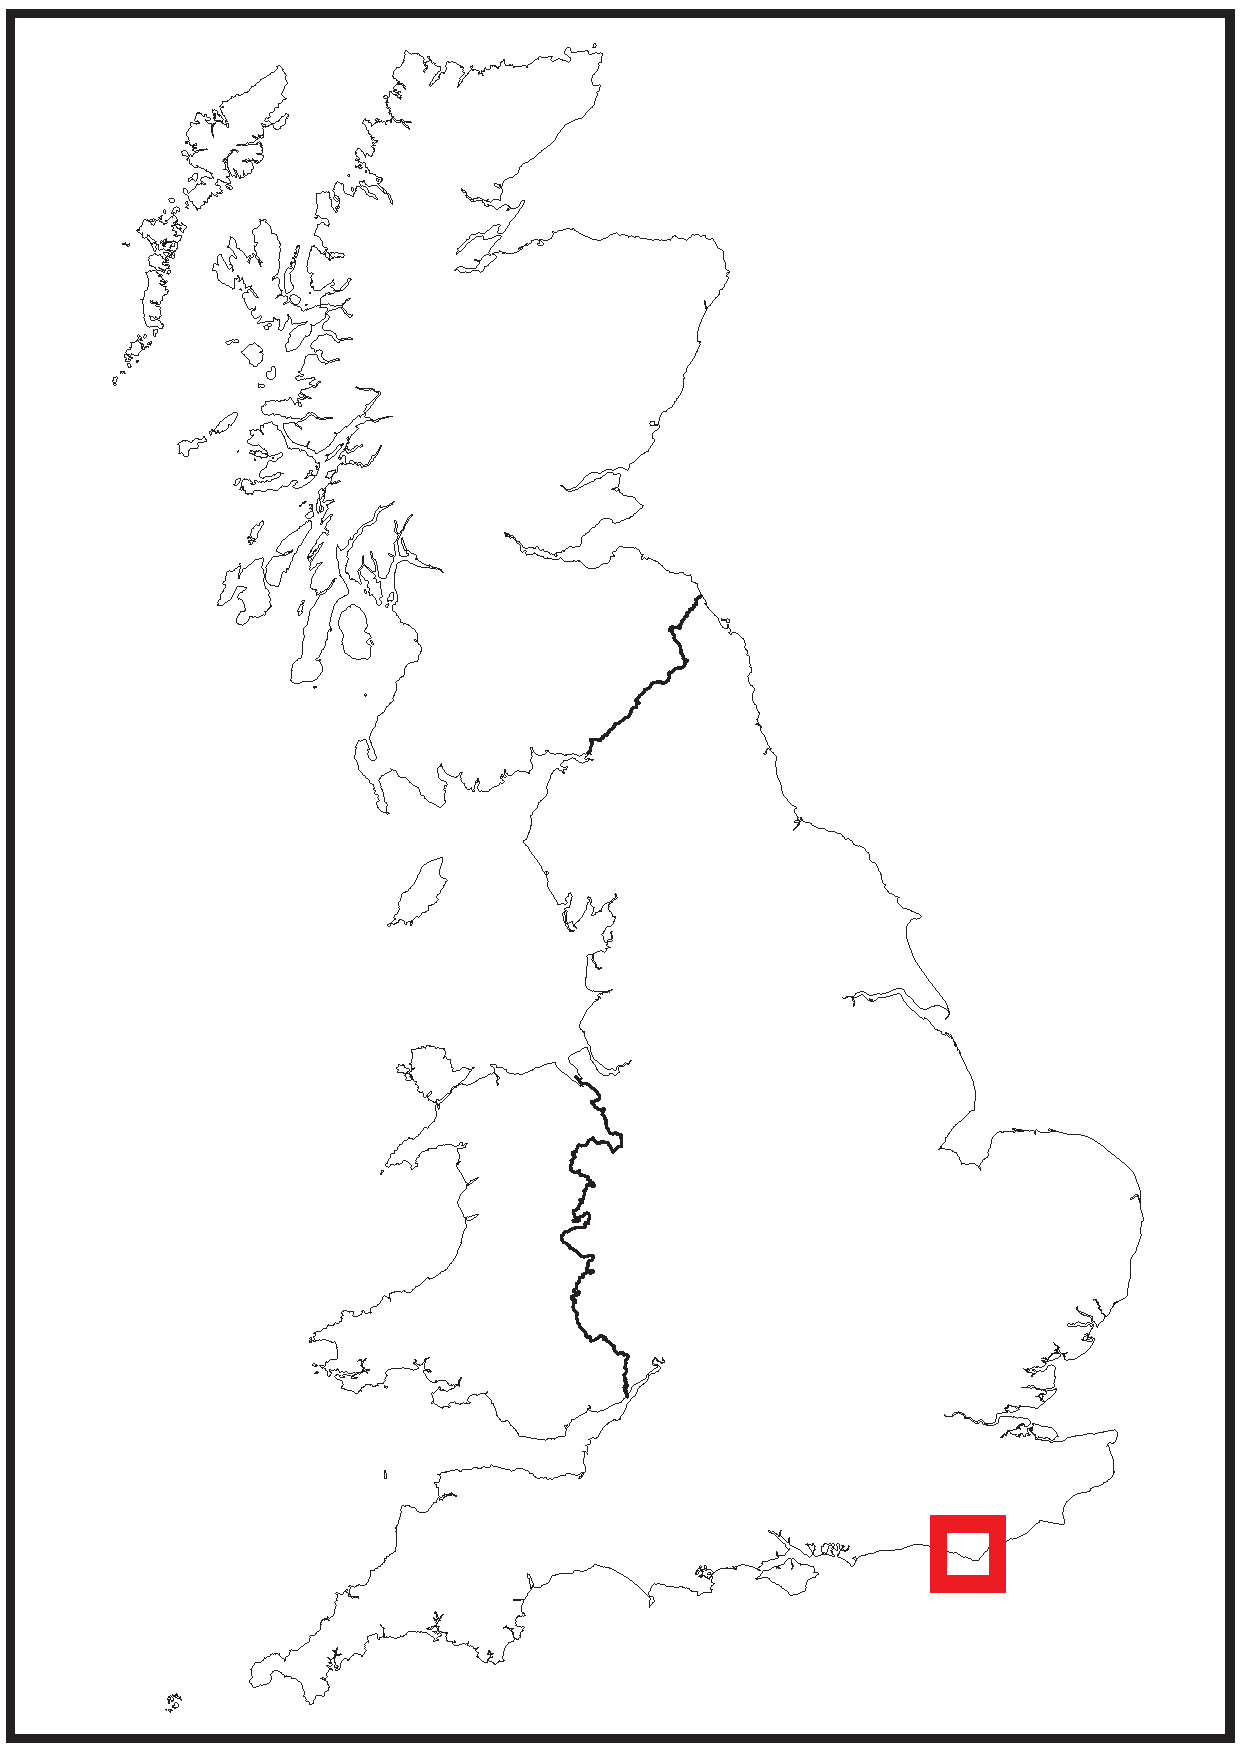
\includegraphics[width=0.19\textwidth]{./img/ukoutline}
  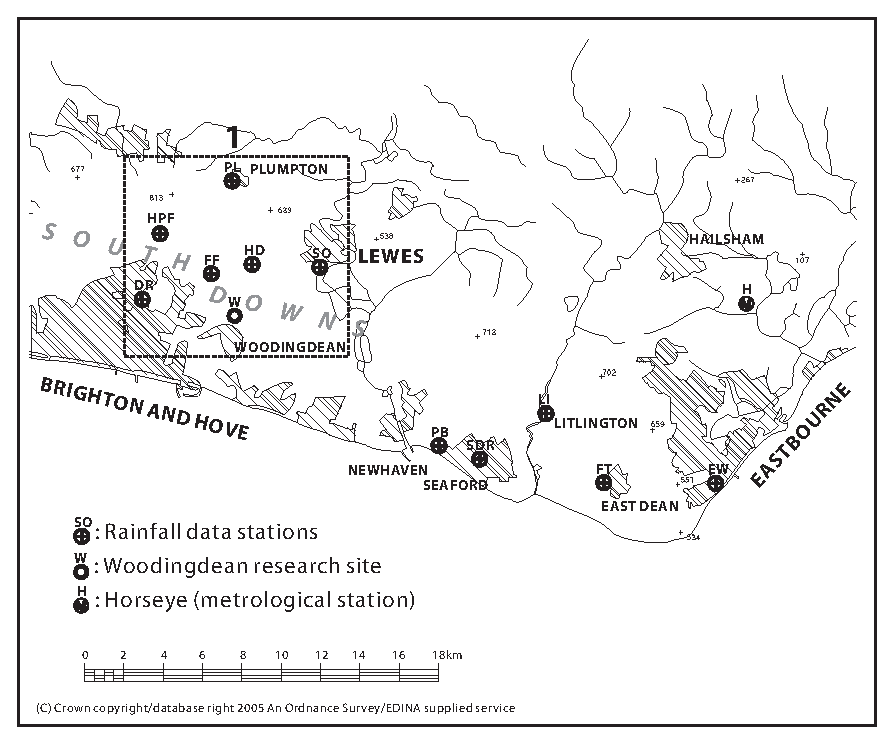
\includegraphics[width=0.8\textwidth]{./img/dailydatasite}
  \caption[Locations of daily rainfall data stations]{Locations of daily
rainfall data stations. DR: Ditchling Road, SO: Southover, PL: Plumpton, SDR:
Seaford D. Road, EW: Eastbourne Wilm., FT: Friston Tower, LI: Litlington, PB:
Poverty Bottom, HPF: High Park Farm, HD: Housedean, FF: Falmer Farm, W:
Woodingdean (soil, slope, crop management), H: Horseye (temperature);
\emph{dotted frame(1)} indicates the area shown in Figure
\ref{fig:EventRainfallDataSite}.}
  \label{fig:DailyRainfallDataSite}
\end{figure}

High resolution event rainfall data measured by tipping-bucket gauges were
obtained from three stations---Ditchling Road, Southover and Plumpton---nearby
the research site (Figure \ref{fig:EventRainfallDataSite}). Detection limit of
the tipping bucket was 0.2 mm. Data duration from each station ranged from 2 to
13 years with some missing data between 1995 and 1998. This might have been
because of vandalisms in the area, a defunct station or temporary gauge
malfunctions (personal communications with Environment Agency on 1 March 2003).
It should be noted that there are only a few rainfall stations which record
event rainfall in the study region (Figure \ref{fig:EventRainfallDataSite}).
Long term high resolution rainfall data with good quality is seldom available
because of, for example, a large size of data file. However, quality of the data
used here was reasonably good of capturing rainfall intensity details.

\begin{figure}[phtb]
  \centering
  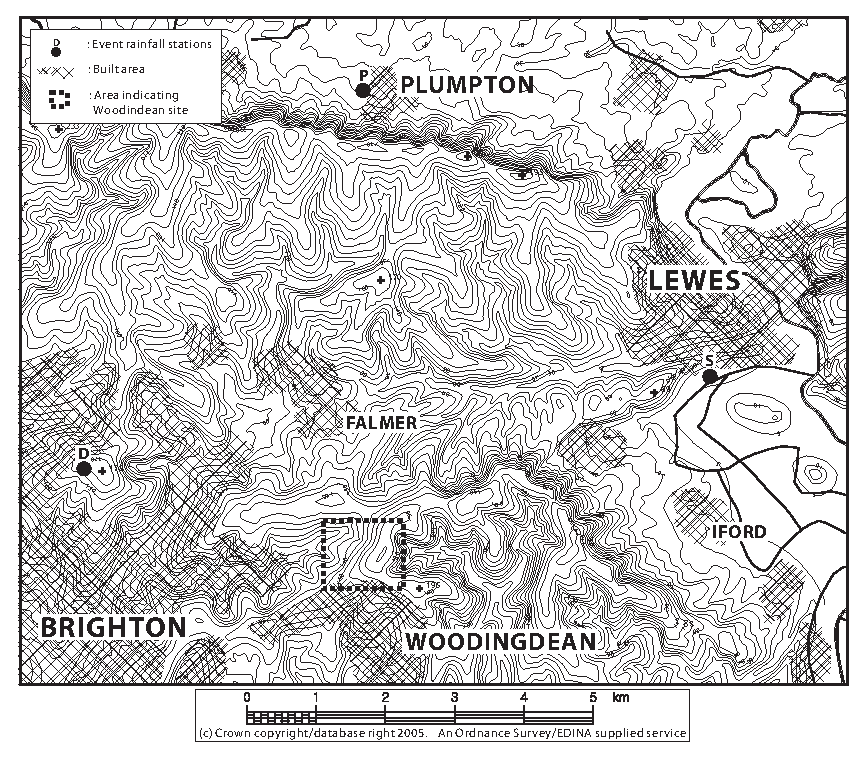
\includegraphics[width=0.8\textwidth]{./img/eventdatasite}
  \caption[Locations of event rainfall data stations]{Locations of event
rainfall data stations. \emph{filled circles}: event rainfall data stations (S:
Southover, D: Ditchling Road, P: Plumpton); Woodingdean site is indicated by
\emph{dotted frame} (see Figure \ref{fig:WoodingdeanSite} for the detail)}
  \label{fig:EventRainfallDataSite}
\end{figure}

The detailed information about the daily and event data are summarised in Table
\ref{tab:DetailsOfDataStations}.

\begin{table}[htbp]
  \figureversion{tabular}
  \centering
  \caption{Details of rainfall data stations}
  \label{tab:DetailsOfDataStations}
    \small
    \begin{tabular}{lllll}
      \toprule
      \textbf{Code} & \textbf{Station} & \textbf{Data type} &
\textbf{Grid reference} & \textbf{Periods}\\
      \midrule
      DR & Ditchling Road & daily & TQ314076 & 1980--1989\\
      SO & Southover & daily & TQ407093 & 1980--1998\\
      PL & Plumpton & daily & TQ356136 & 1980--2000\\
      SDR & Seaford D. Road & daily & TV491993 & 1980--2000\\
      EW & Eastbourne Wilm. & daily & TV611980 & 1980--2000\\
      FT & Friston Tower & daily & TV551982 & 1980--2000\\
      LI & Litlington & daily & TQ523020 & 1980--2000\\
      PB & Poverty Bottom & daily & TQ467002 & 1980--2000\\
      HPF & High Park Farm & daily & TQ331115 & 1974--2004\\
      HD & Housedean & daily & TQ369093 & 1967--2004\\
      FF & Falmer Farm & daily & TQ342084 & 1904--2002\\
      S & Southover & event & TQ407093 &
1993--2001$^\dagger$\\
      D & Ditchling Road & event & TQ315077 &
1991--2003$^\ddagger$\\
      P & Plumpton & event & TQ357135 & 2000--2002\\
      \bottomrule
%     \addlinespace[1mm]
      \multicolumn{5}{l}{\footnotesize $^\dagger$  with
missing data between Sep. 1996 to Jun. 1998}\\
      \multicolumn{5}{l}{\footnotesize $^\ddagger$  with
missing data between Feb. 1995 to Sep. 1997}
    \end{tabular}
\end{table}

\subsection{Other Data}
\label{sec:OtherData}

\subsubsection{Soil}
\label{sec:Soil}

Other input data, such as soil properties and slope profiles, were either
directly acquired from previous studies \citep{favis-mortlock1998-141} or
calibrated as shown in Table \ref{tab:HydrologicalAndErosionalParameters}.
Unless it was critically necessary, all the data were kept unchanged. This
minimizes unknown effects which may occur because of changing other erosional
factors, and also permits the present research to concentrate on the effect of
rainfall intensity changes.

The erosion simulation site is 7.7 ha in size, and is located at Drove Road,
Woodingdean (NGR: TQ358069): this is in the UK South Downs, about 6 km southwest
of Lewes (Figure \ref{fig:WoodingdeanSite}). Soil, slope and crop management
details are obtained from this site.

\begin{figure}[phtb]
  \centering
    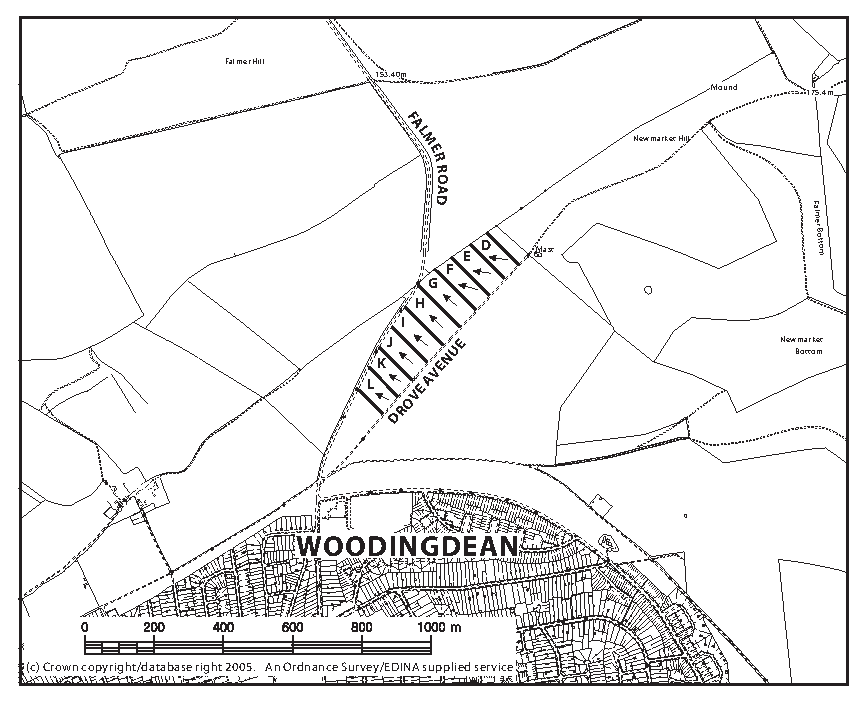
\includegraphics[width=0.8\textwidth]{./img/woodingdean}
  \caption[Woodingdean site]{Woodingdean site. The arrows indicate
approximate downslope direction. Each letter (D-L) denotes hillslope profiles
used for model simulations.}
  \label{fig:WoodingdeanSite}
\end{figure}

The soil in the area is shallow (around 20 cm to chalk) and stony silty rendzina
of the Andover series \citep{jarvis1984-soils}. The Andover silt loams of the
South Downs are both stony and prone to crusting. All the soil input parameters
are summarised in Table \ref{tab:AndoverSoilDetails} and Table
\ref{tab:HydrologicalAndErosionalParameters}.

\begin{table}[htbp]
  \figureversion{tabular}
  \centering
  \caption[Andover soil details]{Andover soil details
\citep[From][]{favis-mortlock1998-141}}
  \label{tab:AndoverSoilDetails}
    \small
    \begin{tabular}{lrrrr}\toprule
    & \multicolumn{4}{c}{Layer}\\
    \cmidrule{2-5}
    & \multicolumn{1}{c}{1} & \multicolumn{1}{c}{2} &
\multicolumn{1}{c}{3} & \multicolumn{1}{c}{4}\\
    \midrule
    Depth to bottom of layer (mm) & 150.0 & 200.0 & 300.0 & 1000.0\\
    Sand (\%) & 18.9 & 18.9 & 25.0 & 25.0\\
    Clay (\%) & 3.5 & 3.5 & 24.0 & 24.0\\
    Organic matter (\%) & 7.0 & 4.8 & 2.2 & 1.2\\
    Cation exchange capacity (meq/100 g of soil) & 45.0 & 39.0 &
30.0 & 14.0\\
    Coarse (Rock) fragments (\% vol) & 38.1 & 50.0 & 90.0 & 90.0\\
    \bottomrule
    \end{tabular}
\end{table}

Values for WEPP's parameters for effective hydraulic conductivity, together with
values for its three erodibility parameters, were subjectively adjusted
following the suggestions by \citet{favis-mortlock1998-141} (Table
\ref{tab:HydrologicalAndErosionalParameters}). The parameters for interrill and
rill erodibility ($K_i$ and $K_r$) were reduced, while the critical shear stress
parameter $\tau_c$ was increased. The value for the base line effective
hydraulic conductivity parameter $K_b$ was also increased. All the adjustments
were taken from \citet{favis-mortlock1998-141} with the exception of critical
shear stress parameter $\tau_c$ which was recalibrated to 6. This was done in
order to meet the recommended value of maximum  $\tau_c$ by the WEPP
documentation. All calibrated values were constrained to remain within the
recommended ranges in WEPP documentation \citep{flanagan1995-usda}.

\begin{table}[htbp]
  \figureversion{tabular}
  \centering
  \caption[Hydrological and erosional parameter values]{Hydrological and
erosional parameter values \citep[After][]{favis-mortlock1998-141}}
  \label{tab:HydrologicalAndErosionalParameters}
    \small
    \begin{tabular}{lrr}
    \toprule
    & Uncalibrated Hydrological & Calibrated Hydrological\\
    & and erosional parameters & and erosional parameters\\
    \midrule
    Effective hydraulic conductivity & &\\
    of top soil layer (mm/hr) & 2.1$^a$ & 3.0$^a$\\
    Interrill erodibility $K_i$ (kg s/m$^4$) & 5502700 & 2000000\\
    Rill erodibility $K_r$ (s/m) & 0.0871 & 0.0050\\
    Critical shear stress $\tau_c$ (N/m$^2$) & 3.5 & 6.0$^b$\\
    \bottomrule
%   \addlinespace[1mm]
    \multicolumn{3}{l}{\footnotesize $^a$ `baseline' effective
hydraulic conductivity for WEPP ($K_b$)}\\
    \multicolumn{3}{l}{\footnotesize $^b$ adjusted to 6 which is a
maximum value for cropland $\tau_c$}
    \end{tabular}
\end{table}

\subsubsection{Management}
\label{sec:Management}
A typical crop management practice for the area is continuous growing of winter
wheat. The typical timing of tillage operation for the area is shown in Table
\ref{tab:TillageOperationTiming}.

\begin{table}[htbp]
  \figureversion{tabular}
  \centering
  \caption[Tillage operation timing at Woodingdean site]{Tillage operation
timing at Woodingdean site \citep[From][]{favis-mortlock1998-141}}
  \label{tab:TillageOperationTiming}
    \small
    \begin{tabular}{lr@{ }l}
      \toprule
      \textbf{Operation} & \multicolumn{2}{l}{\textbf{Date}}\\
      \midrule
      Chisel plough & 20 & August\\
      Harrow & 15 & September\\
      Drill (Winter wheat) & 28 & September\\
      Roll & 1 & October\\
      Harvest & 29 & July\\
      \bottomrule
    \end{tabular}
\end{table}

\subsubsection{Topography}
\label{sec:TopographyData}
Slope angles in the site range from 12 to 20\%, with a convexity toward the
centre. The site was divided into nine sub-areas for modelling, approximately
down the line of greatest slope, which faces a northwesterly direction (Figure
\ref{fig:WoodingdeanSite}). The length of each slope varies from 125 to 180
metres, and width is 50 metres for all the slopes.

\subsubsection{Temperature}
\label{sec:Temperature}

Daily temperature records for 1990--2000 were obtained from Horseye Station
(NGR: TQ627083) (Figure \ref{fig:DailyRainfallDataSite}). The distance of this
station from the study site is about 25 km. This data set was used in this study
since no other data set was available from the region at that time. Average
annual maximum and minimum temperature are 14.9\textcelsius\ (SD:
5.5\textcelsius)\ and 6.6\textcelsius\ (SD: 4.9\textcelsius), respectively.

\section{Justification for Erosion Model Selection}
\label{sec:ModelConfiguration}

As the research aims to investigate impacts of extreme rainfall events, all soil
erosion models used in this research should be able to simulate a single erosion
event. WEPP, EUROSEM and RillGrow were chosen because of this reason. All three
models are capable of simulating single events while WEPP may also be used for
continuous simulations (Table \ref{tab:ModelsUsedInThePresentStudy}).

There are two more reasons why these models were used. One is that they use
different approaches to erosion simulations and rainfall intensity. WEPP, for
example, estimates soil erosion using steady-state approach
(Equation \ref{eq:weppsedimentload}) while EUROSEM employs a dynamic approach
using a mass balance equation (Equation \ref{eq:eurosemmassbalance}).
Both models also consider rill and interrill areas separately and use
different equations for describing processes in two areas. In terms of
rainfall intensity, WEPP uses rainfall intensity as effective rainfall
intensity for estimating interrill erosion. In EUROSEM rainfall intensity is
considered as a function of kinetic energy of raindrops which act as detachment
agents of soil particles.
RillGrow, on the other hand, is based on a
self-organising dynamic system to simulate the initiation and development of a
network of rills. RillGrow also does not consider rill and interrill areas
separately. All three models are described previously (Section
\ref{sec:SoilErosionPredictionModels}).
The other reason why these models were used is that they are
originally designed for different simulation scales, temporally and spatially.
Table \ref{tab:ModelsUsedInThePresentStudy} summarises some features of these
three models.

Comparing the outputs from three erosion models could reveal strengths and
weaknesses of their approaches to soil erosion. In turn, this investigation may
provide improved insights on the behaviour of the models in relation to rainfall
intensity changes.

\begin{sidewaystable}[htbp]
  \centering
  \caption{Summary of the erosion models used in this research}
  \label{tab:ModelsUsedInThePresentStudy}
    \begin{tabular}{llll}
\toprule
    & WEPP      & EUROSEM   & RillGrow\\
\midrule
Spatial Scale & small catchment,  & small catchment,  & small field,\\
    & hillslope,    & hillslope,  & laboratory plot\\
    & individual field  & individual field  & \\
\midrule
      Reference & \citealp{nearing1989-1587} &
\citealp{morgan1998-389} & \citealp{favis-mortlock1998-353}\\
                & \citealp{flanagan1995-usda} & & \\
      \midrule
      Purpose  & event-based erosion & event-based erosion &
rill initiation\\
               & transport and deposition & transport and
deposition & and development\\
               & long-term simulation & & \\
      \midrule
      Approach & Steady-state & Dynamic & Self-organising dynamic\\
      \midrule
      Required Data & soil erodibility, & soil erodibility, &
detailed surface micro-\\
                    & slope profile & surface characteristics
& topography, soil type \\
                    & and crop management   & and plant cover
& and rainfall intensity  \\
      \midrule
      Rainfall Intensity & Yes (effective) & Yes (kinetic energy) & Yes \\
      \midrule
      Simulation Type & single event or continuous & single
event & single event\\
      \bottomrule
    \end{tabular}
\end{sidewaystable}

WEPP was selected partly because it has been widely used and studied
\citep{zhang1996-855,baffaut1998-756,favis-mortlock1999-329,pruski2002-climate,
pruski2002-7,flanagan2007-1603}, so there is a substantial amount of
information to compare it with. Moreover, when WEPP was developed, it was
implemented with an unique method (or sub-model) of describing and utilizing
rainfall data, called CLIGEN. This feature has been described previously in
Section \ref{sec:ClimateGeneratorCLIGEN}. The second model, EUROSEM, was
selected because it was developed with European conditions in mind, as its name
may imply (i.e.\ \emph{EUR}opean \emph{S}oil \emph{E}rosion \emph{M}odel) (See
Section \ref{sec:EuropeanSoilErosionModelEUROSEM} for review). In this regard,
EUROSEM may provide a good comparison to WEPP, which has been developed mainly
with datasets collected from the USA \citep{flanagan2007-1603}. Lastly, RillGrow
was employed in the later stage of the research in order to generate stronger
consensus from an additional model. RillGrow's unique approach (i.e.\ a
self-organising dynamic systems approach) to soil erosion simulation (See
Section \ref{sec:ModelDescriptionRillGrow}) is also another reason for the
selection. RillGrow simulates erosion on a finer scale using iterations of
erosion estimations by a single raindrop at a time. This also gives a good
comparison to the former two models.


%
%
%$\filledstar\filledstar\filledstar$ Rationalising reason for selecting
%three models
%
%$\filledstar\filledstar\filledstar$ Contrast the models (in relation to the
%inputs as a table)
%
%\subsection{WEPP}
%\label{sec:WEPP}
%version and input data (+initial condition)
%WEPP simulation settings and assumptions.
%
%\paragraph{CLIGEN}
%\label{sec:CLIGEN}
%version and input data
%
%\begin{table}[htbp]
% \centering
% \caption[Original and Updated MEAN~P for Ditchling Road]{Original and
%Updated MEAN~P for Ditchling Road (inches)}
% \label{tab:UpdatedMEANPForDitchlingRoad}
%   \footnotesize
%   \begin{tabular}{lrrrrrrrrrrrr}
%   \toprule
%    & Jan & Feb & Mar & Apr & May & Jun & Jul & Aug & Sep & Oct &
%Nov &
%Dec\\
%   \cmidrule{2-13}
%   Original & 0.19 & 0.16 & 0.17 & 0.16 & 0.16 & 0.20 & 0.19 & 0.22
%& 0.23
%& 0.27 & 0.21 & 0.20\\
%   Updated & 0.11 & 0.11 & 0.18 & 0.21 & 0.17 & 0.15 & 0.16 & 0.13
%& 0.24 &
%0.29 & 0.19 & 0.29\\
%   \bottomrule
%   \end{tabular}
%\end{table}
%
%\begin{figure}[htbp]
% \centering
%   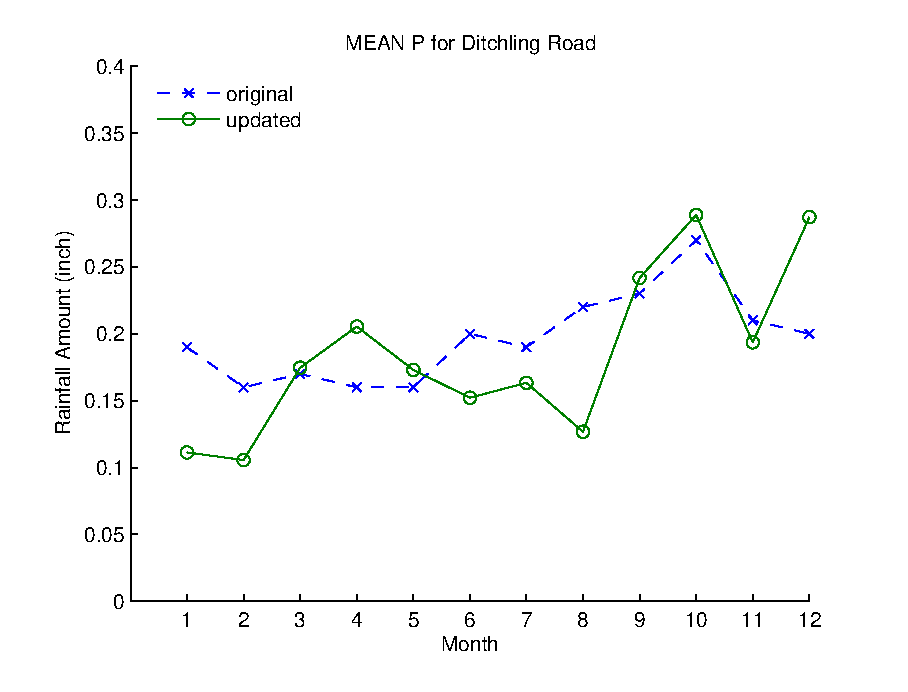
\includegraphics[width=0.60\textwidth]{mean_p_cligen}
% \caption[Mean daily precipitation depth]{Mean daily precipitation depth
%(inch)}
% \label{fig:mean_p_cligen}
%\end{figure}
%
%peak amount in autumn
%
%\begin{table}[htbp]
% \centering
% \caption[Original and Updated MX~.5P for Ditchling Road]{Original and
%Updated MX~.5P for Ditchling Road (in/hr)}
% \label{tab:UpdatedMX5PForDitchlingRoad}
%   \footnotesize
%   \begin{tabular}{lrrrrrrrrrrrr}
%   \toprule
%    & Jan & Feb & Mar & Apr & May & Jun & Jul & Aug & Sep & Oct &
%Nov & Dec\\
%   \cmidrule{2-13}
%   Original & 0.63 & 0.59 & 0.55 & 0.55 & 0.55 & 0.55 & 0.55 & 0.67
%& 0.79 & 0.93 & 0.87 & 0.75\\
%   Updated & 0.27 & 0.18 & 0.23 & 0.23 & 0.27 & 0.33 & 0.42 & 0.58
%& 0.43 & 0.45 & 0.34 & 0.30\\
%   \bottomrule
%   \end{tabular}
%\end{table}
%
%\begin{figure}[htbp]
% \centering
%   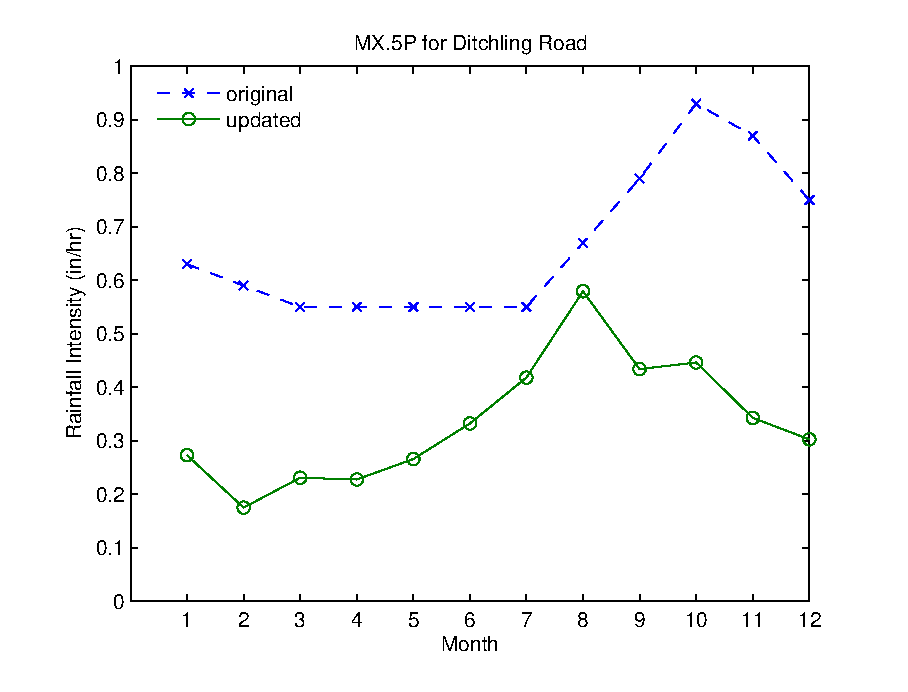
\includegraphics[width=0.70\textwidth]{mx5p_cligen}
% \caption[Mean max. daily 30-minute rainfall intensity]{Mean max. daily
%30-minute rainfall intensity (in/hr). High intensity event in summer}
% \label{fig:mx5p_cligen}
%\end{figure}
%Complete input files for both sites are shown in Appendix
%\ref{sec:CLIGENInputData}.
%
%\subsection{EUROSEM}
%\label{sec:EUROSEM}
%
%EUROSEM input settings and assumptions.
%
%\subsection{RillGrow}
%\label{sec:ModelConfigurationRillGrow}
%
%RillGrow input settings and assumptions.

\section{A Brief Overview of Research Method}
\label{sec:OverviewOfResearchMethods}

This research aims to discover how rainfall intensity changes will affect the
soil erosion rate in the future, using soil erosion models. The research method
involves data acquisition, such as observed rainfall properties and soil
properties, configuring erosion models, and sensitivity tests of erosion models.
The simulation carried out for the sensitivity test mainly employs a univariate
method.

% As this study mainly aims to investigate soil erosion changes as a response
%to future rainfall intensity changes, and future rainfall intensity changes are
%still poorly known, it is not the main focus of this study to actually attempt
%to predict future soil erosion rates. Instead, this study aims to investigate
%the way in which rainfall intensity changes can affect soil erosion rates.
%Greater knowledge here will, once future changes in rainfall intensity become
%better known, improve our ability to estimate future rates of erosion. Thus, in
%general, a ``sensitivity analysis'' approach is followed. ``Known'' rather than
%``realistic'' changes in intensity are used in this thesis.

%The thesis consists of 11 chapters in total. These chapters are divided into
%five parts: Introduction, Observed Precipitation of the Research Site, Rainfall
%Intensity Changes and Soil Erosion, Implications of Climate Change on Future
%Soil Erosion, and Conclusion.
Three soil erosion models, WEPP (Water Erosion Prediction Project), EUROSEM
(EURopean Soil Erosion Model), and RillGrow were used to simulate runoff and
erosion rate under various rainfall intensity conditions. Effects of temporal
resolution of rainfall data on runoff and soil loss generations are investigated
to identify requirements of rainfall intensity information for erosion
simulations. Two extreme rainfall events; one with highest rainfall intensity
and the other with highest rainfall amount, were selected from the
tipping-bucket rainfall data. Tipping-bucket data for the events are then
aggregated into a range of different temporal ``scales". This is done by the
discretization of tipping-bucket data into rainfall data that have a range of
time-steps (i.e. 1, 5, 15, 30 and 60min).
Runoff and soil loss rates were simulated using three models with these rainfall
input data. An additional rainfall event, which has both wet and dry phases
during the storm period, was selected. Two rainfall input data were prepared
from this event data; one without any alteration and the other that is
aggregated into a continuous storm by removing dry phases during the storm.
Runoff and soil loss rates were simulated using three models with these two
additional rainfall inputs. This was done to investigate effects of the dry
phase within a storm on soil erosion. Impacts of various rainfall intensities
patterns on soil erosion were also studied using rainfall data from a designed
storm. Four different storms that have increasing, increasing-decreasing,
decreasing and constant rainfall intensity were prepared for erosion
simulations. Rainfall amounts for all four storms were kept the same while the
intensities vary.

To understand observed trends of rainfall intensity changes, three observed
precipitation data (i.e.\ Monthly 0.5\textdegree\ grid data, daily station data
and tipping-bucket gauge data) were acquired from the South Downs, UK. Monthly
0.5\textdegree\ grid data for 100 years were analysed, firstly, to draw outlines
of long term rainfall trends in the area. Daily precipitation data from 11
stations for the various observational periods (i.e.\ 9--93 years) in the area
were then analysed, in terms of:
\begin{itemize*}
 \item daily rainfall amount,
 \item number of raindays,
 \item simple daily intensity index,
 \item number of raindays with rainfall amount $\geq$10 mm, and
 \item number of raindays with rainfall amount $\geq$20 mm.
\end{itemize*}
This gave more detailed information about the trends of rainfall in the region
than that obtained from monthly 0.5\textdegree\ grid data. Lastly, even greater
detailed rainfall trends were studied using tipping-bucket collected rainfall
data from three stations over the period of 2--13 years. This kind of high
resolution data provides very detailed information on the patterns of the
rainfall amount and intensity.

Likely future soil erosion rates were estimated only using WEPP, as the other
two models are not designed for continuous long term simulations. A hundred
year-long weather is generated by the WEPP's climate component called CLIGEN
(CLImate GENerator) as a control climate dataset. Rainfall intensity was
then increased proportionally from the control data by changing rainfall
duration, keeping rainfall amount constant. Runoff and erosion rates were
simulated using these climate data.

\subsection{Statistical Methods for Trend Investigation}
\label{StatisticalMethodsForTrendInvestigation}

Statistical methods used in this research are briefly summarized here.

\paragraph{Simple Linear Regression}
\label{sec:SimpleLinearRegression}

%REGRESSION OR CORRELATION?
%
%Select the Pearson (parametric) correlation coefficient if you can assume
%that both X and Y are sampled from Gaussian populations. Otherwise choose
%the Spearman nonparametric correlation coefficient. Don't calculate the
%correlation coefficient (or its confidence interval) if you manipulated the
%X variable.

%Calculate linear regressions only if one of the variables (X) is likely to
%precede or cause the other variable (Y). Definitely choose linear
%regression if you manipulated the X variable. It makes a big difference
%which variable is called X and which is called Y, as linear regression
%calculations are not symmetrical with respect to X and Y. If you swap the
%two variables, you will obtain a different regression line.

Linear regression function ($y=\alpha + \beta x$) was assumed where rainfall
related indicators (Table \ref{tab:RainfallIntensityIndicators}) as dependent
variables ($y$) and time as a independent variable ($x$). The regression
coefficient ($\beta$) might be used to detect trends in time series of the
indicators. The Student's $t$-test was used to test whether the trend is
statistically significant.

%If $t$-value is greater than 1.96 ($n=\infty$), reject null hypothesis
%($\beta = 0$) with $95\%$ confidence level.
%If $n=5$, $\bar{x}\pm2.776 \frac{\sigma}{n^{1/2}}$ ; if N=10: Xavg$\pm$
%2.262 sdev/N1/2 ; if N=20: Xavg$\pm$ 2.093 sdev/N1/2 ; if N=40; Xavg$\pm$
%2.023 sdev/N1/2 ; and for ``arge'' N: Xavg$\pm$ 1.960 sdev/N1/2


\paragraph{Mann-Kendall's Test}
\label{sec:MannKendallSTest}

Mann-Kendall's test is a non-parametric test for the detection of trend in a
time series. This is primarily used because it has no linearity assumption.
Since the first proposals of the test by \citet{mann1945-245} and
\citet{kendall1975-202}, covariances between Mann-Kendall statistics were
proposed by \citet{dietz1981-169} and the test was extended in order to include
seasonality \citep{hirsch1984-727}, multiple monitoring sites
\citep{lettenmaier1988-505} and covariates representing natural fluctuations
\citep{libiseller2002-71}.

%This section should be about Kendall's rank correlation.
%look at the matlab script!

The Mann-Kendall rank correlation \citep{mann1945-245,kendall1975-202} is
sensitive to both linear and non-linear trends. This is a non-parametric method
and is based on ranking of a time series, using only the relative ordering of
ranks \citep{press1996-933}. It does not give any information about the
magnitude of the trend in the actual time series but rather gives a significance
of the trend, and information on the direction of the observed trend (i.e.\
upward, downward or unchanged).

%\begin{equation}
%\label{eq:Tau}
% T=\sum^{N}_{i=1}n_i
%\end{equation}
%where, $N$ is the total number of element in the data set (no. of years).
%$n_i$ is the number of preceding element that is larger than element $x_i$
%(i=1,2,\ldots $N$).
%When $N$ is greater than 10, the distribution function of $T$ (test
%variable) is assumed to be asymptotically Gaussian.
%
%Thus, expected value, $E(T)$ is given by:
%
%\begin{equation}
%\label{eq:ExpectedTau}
% E(T)=\mu=\frac{N(N-1)}{4}
%\end{equation}
%and, variance, $var(T)$ is given by:
%
%\begin{equation}
%\label{eq:VarianceTau}
% var(T)=\sigma^2=\frac{N(N-1)(2N+5)}{72}
%\end{equation}
%The normalised test variable, $Z(T)$, is given by:
%
%\begin{equation}
%\label{eq:NormalisedTestVariable}
% Z(T)=\frac{T-E(T)}{\sqrt{var(T)}}
%\end{equation}
%
%If $|Z(T)| > 1.96$, $H_0$ shall be rejected with $95\%$ confidence level.
%When $Z(T)$ is significant, $Z(T) > 0$ or $Z(T) < 0$ defines an ascending
%or descending trend.

\paragraph{Kolmogorov-Smirnov test}
\label{sec:KolmogorovSmirnovTest}
The two sample Kolmogorov-Smirnov test is used to determine if two distributions
differ significantly. The K-S test is a non-parametric test that tests
differences between two distributions. The K-S test has the advantage of making
no assumption about the distribution of data. Its null hypothesis is that the
two samples are distributed identically. The test is sensitive to differences in
location, dispersion and skewness of the distribution \citep{sokal1995-887}.

%\begin{verbatim}
%http://en.wikipedia.org/wiki/Kolmogorov-Smirnov_test
%\end{verbatim}
%09:06, 13 September 2006
%
%$\downarrow$ need to be reworded
%
%In statistics, the Kolmogorov-Smirnov test (often called the K-S test) is
%used to determine whether two underlying probability distributions differ,
%or whether an underlying probability distribution differs from a
%hypothesized distribution, in either case based on finite samples.
%
%The one-sample KS test compares the empirical distribution function with
%the cumulative distribution function specified by the null hypothesis. The
%main applications are testing goodness of fit with the normal and uniform
%distributions. For normality testing, minor improvements made by Lilliefors
%lead to the Lilliefors test. In general the Shapiro-Wilk test or
%Anderson-Darling test are more powerful alternatives to the Lilliefors test
%for testing normality.
%
%The two-sample KS test is one of the most useful and general nonparametric
%methods for comparing two samples, as it is sensitive to differences in
%both location and shape of the empirical cumulative distribution functions
%of the two samples.
%
%empirical distribution function Fn for n observations yi is defined as
%
%\begin{equation}
% F_n(x)={\frac{1}{n}}\sum_{i=1}^n \left\{\begin{matrix}1 & \mathrm{if}\
%y_i\leq x, \\ 0 & \mathrm{otherwise}.\end{matrix}\right.
%\end{equation}
%
%The two one-sided Kolmogorov-Smirnov test statistics are given by
%
%\begin{equation}
% D_n^{+}=\max(F_n(x)-F(x))
%\end{equation}
%\begin{equation}
%     D_n^{-}=\max(F(x)-F_n(x))
%\end{equation}
%
%where F(x) is the hypothesized distribution or another empirical
%distribution. The probability distributions of these two statistics, given
%that the null hypothesis of equality of distributions is true, does not
%depend on what the hypothesized distribution is, as long as it is
%continuous.
%
%Knuth gives a detailed description of how to analyse the significance of
%this pair of statistics [citation needed]. Many people use max(Dn+, Dn-)
%instead, but the distribution of this statistic is more difficult to deal
%with.
%
%
%When the underlying independent variable is cyclic, as with day of the year
%or day of the week, then Kuiper's test is more appropriate. Numerical
%Recipes is a good source of information on this.
%
%Furthermore, the Kolmogorov-Smirnov test is more sensitive at points near
%the median of the distribution than at its tails. The Anderson-Darling test
%provides equal sensitivity at the tails.

%******This part may need to be more descriptive
%
%The research described here involves three strategic stages:
%\begin{quote}
% \begin{enumerate}
%   \item Investigation of Rainfall Intensity
%   \item Erosion Model Evaluation
%   \item Estimation of Future Soil Erosion
% \end{enumerate}
%\end{quote}
%
%For the first stage, three temporally and spatially different datasets
%(i.e.\ monthly 0.5\textdegree\ grid data, daily station data and
%tipping-bucket gauge data) are investigated to find trends in rainfall
%intensity changes.
%In the second stage, Erosion Model Evaluation assesses soil erosion models
%(e.g.\ WEPP and EUROSEM) to find out their responses to rainfall intensity
%changes. The changes in rainfall intensity are accomplished by changing the
%original intensity proportionally. This stage provides information on
%differences between the models' responses compared to real erosion system's
%responses to changed rainfall intensity.
%At the final stage, the outcomes from the previous two stages provide
%information on future rainfall intensity, and erosion model response to
%rainfall intensity changes. This information is then used to estimate
%likely ranges of future rainfall intensity changes. In turn, future soil
%erosion rate are estimated.
%
%This research may expect following outcomes:
%\begin{quote}
% \begin{enumerate}
%   \item Improvement of our understandings of rainfall intensity
%   \item Requirement of rainfall intensity information for soil
%erosion estimation
%   \item Identification of limitations of soil erosion models for
%incorporating future rainfall intensity changes
%   \item Suggestions for soil erosion model improvements
%   \item Estimation of future soil losses induced by rainfall
%intensity changes
% \end{enumerate}
%\end{quote}

%\nolinenumbers
%\linenumbers*
\chapter{OBSERVED RAINFALL CHARACTERISTICS OF THE STUDY AREA}
%\section{Observed Rainfall Characteristics Of The Study Area}
\label{sec:RainfallCharacteristicsOfTheStudyArea}

%This chapter should really focus on comparing observed intensity trends with
%what is predicted for the future---not \emph{just} looking at trends, but
%seeing how well those trends are consistent with, or different from, GCM
%predictions for the future. You should mention that here.

\section{Introduction}
\label{sec:ObservedRainfallIntroduction}
%******In this chapter, why observed data were analysed is to be explained.
%Also, I need to indicate what are the possible benefits taking this route
%rather than other ways such as downscaling or perturb with GCM (or RCM)
%outputs.
As stated previously, it became apparent at the early stage of this research
that RCM rainfall data could not (and still cannot) be used directly for erosion
simulations. Although RCMs and empirically downscaled data from GCMs allow
projections to be made at a finer resolution than GCMs, RCM projections
still vary
greatly between models in the same way as GCMs and empirical downscaling does
not attempt to correct any biases in the data from the GCMs. Even with a finer
resolution than GCMs, RCM data do not hold sufficiently detailed information of
rainfall intensity that can be used directly for erosion simulations, and were
not reliable enough for this type of approach yet---and still they are not
\citep{nearing2001-229,michael2005-155,o'neal2005-165}. That is why this part of
research was carried out.

Moreover, using outputs from a model as inputs to another model will increase
the level of uncertainty because there may be compound errors originated from
both models. For example, when RCMs generate future rainfall data, these
rainfall data are in a wrong resolution, that is a larger resolution than what
is needed
for erosion simulations. Also, rainfall intensity data that have been obtained
from these RCM-generated rainfall data will be in a wrong resolution. This
resolution
mis-match induces the use of downscaling to make the data usable for soil
erosion modelling. During these processes, the level of uncertainty will
increase process after process. Therefore, using observed rainfall data for
erosion simulations may be more beneficial than using RCM data. It certainly is
easier to track errors from known sources such as observed rainfall data, too.

The limitation of using observed data would be that it needs correctly scaled
data to begin with and needs reasonably long data duration to be able to pick up
seasonal variations at least, if not greater. Also, it should be remembered that
this approach is to create scenarios of future rainfall which are based on
present-day rainfall, not future rainfall. Thus, this approach assume that
future rainfall trends stay the same as present-day rainfall trends.
%Is the future rainfall intensity going to be different from the present? If so,
%how is it going to be different? Is it going to increase---or decrease?

In this chapter, three different scales of observed rainfall records were
analysed to find the rainfall intensity trend---Monthly 0.5\textdegree\ grid
rainfall, daily station rainfall and event rainfall measured by tipping-bucket
gauges. The descriptions of these data are covered in Section \ref{sec:Data}.

\section{Method}
\label{sec:MethodsObservedRainfallCharacteristicInvestigation}
%(***REFS NEEDED to back this up, for example, refs that used observation to
%estimate trends and method I used.) %(***NOTE TO SELF Emphasise that it has
%been done before and proven, also say about pros and cons. in discussion)
All three datasets described previously (Table
\ref{tab:PrecipitationDataUsedForCurrentRainfallTrendInvestigation}) were
analysed to find out rainfall intensity trends in the area using simple linear
regression and Mann-Kendall (M-K) rank correlation. Monthly 0.5\textdegree\ grid
rainfall data and daily station rainfall data were used without any conversion.
Event rainfall data recorded by a tipping-bucket gauge are analysed.
Tipping-bucket gauge rainfall data were aggregated into 1-min rainfall data
prior to use. Rainfall amount, duration and daily maximum 1-min peak intensity
were investigated using 1-min event rainfall data.

\citet{kundzewicz2004-7} suggested a number of tests for trend detection:
Spearman's rho, Kendall's tau/Mann-Kendall test, Seasonal Kendall test, Linear
regression and other robust regression tests.
\citet{hannaford2006-1237} also used three methods (i.e.\ M-K rank, Spearman's
rho and linear regression) to assess trends in UK runoff and low flows. They
found a good agreement between the detection rate of trends between the three
trend-testing methods.
More studies have observed a high degree of equivalence between M-K rank and
Spearman's rho tests \citep{yue2002-254} and M-K rank and linear regression
\citep{svensson2005-811}

\citet{yue2002-254} investigated the power of M-K rank and Spearman's rho. They
found that both have similar power in detecting a trend to the point of being
indistinguishable in practice. \citet{yue2002-254} said ``The power of M-K rank
test depends on the pre-assigned significance level, magnitude of trend, sample
size, and the amount of variation within a time series. That is, the bigger the
absolute magnitude of trend, the more powerful are the tests; as the sample size
increases, the tests become more powerful; and as the amount of variation
increases within a time series, the power of the tests decrease. When a trend is
present, the power is also dependent on the distribution type and skewness of
the time series.''

Thus, two trend test methods, that are linear regression and M-K rank, are used
in this section.

The trends in daily rainfall characteristics were investigated. Rainfall related
indicators were calculated to determine rainfall characteristics (Table
\ref{tab:RainfallIntensityIndicators}). Daily rainfall intensity is obtained by
dividing the monthly rainfall amount by the number of raindays.

\begin{table}[htbp]
  \figureversion{tabular}
  \centering
  \caption{Rainfall intensity indicators}
  \label{tab:RainfallIntensityIndicators}
  \footnotesize
    \begin{tabular}{l p{95mm} l}
    \toprule
    \textbf{Indicator} & \textbf{Definition} & \textbf{Unit}\\
    \midrule
    RR & Precipitation sum & mm\\
    RR1 & Number of wet days (RR $\geq$ 1 mm/day) & days\\
    SDII & Simple daily intensity index: \[\frac{\textrm{total
rainfall amount for wet days (RR $\geq$ 1 mm/day)}}{\textrm{number of wet days}}
\] & mm/day\\
    %\addlinespace[-2.5mm]
    R10mm & No. of days with precipitation $\geq$ 10 mm/day & days\\
    R20mm & No. of days with precipitation $\geq$ 20 mm/day & days\\
    R10p$^\dagger$ & Ratio of days with precipitation $\geq$ 10
mm/day ((R10/RR1)$\times100$) & \%\\
    R20p$^\dagger$ & Ratio of days with precipitation $\geq$ 20
mm/day ((R20/RR1)$\times100$) & \%\\
    \bottomrule
%   \addlinespace[1mm]
    \multicolumn{3}{p{12cm}}{\footnotesize $^\dagger$\ Additional
indicators, which are not listed in the European Climate Assessment \& Dataset
project (ECA\&D) website. Complete list of indicators and their definitions are
available at http://eca.knmi.nl/indicesextremes/indicesdictionary.php}
    \end{tabular}
\end{table}

Any year with partial records were discarded to minimize the effects from
missing data (Table \ref{tab:DailyRainfallStationsAndRecordDetails}).
The records of the last year of each station were also discarded as they are
incomplete. For example, daily rainfall data from Falmer Farm (FF) were
considered only for 1904--1996 discarding the records for 1997 and 1999 with
missing data. Three more years (1998, 2000 and 2001) were discarded from all the
stations because of the discontinuity resulted in by removing missing data
periods. Also, there was a problem with 2000 rainfall because they were recorded
as weekly total rather than daily total.

\begin{table}[htbp]
  \figureversion{tabular}
  \centering
  \caption{Daily Rainfall Stations and Record Details }
  \label{tab:DailyRainfallStationsAndRecordDetails}
  \small
    \begin{tabular}{llll} \toprule
    \textbf{Code} & \textbf{Station Name} & \textbf{Periods}* &
\textbf{Studied Periods}*\\
    \midrule
    DR & Ditchling Road & 1980--1989 (10) & 1980--1988 (9)\\
    SO & Southover & 1980--1998 (19) & 1980--1997 (18)\\
    PL & Plumpton & 1980--2000 (21) & 1980--1998 (19)\\
    PB & Poverty Bottom & 1980--1998 (19) & 1980--1997 (18)\\
    SDR & Seaford D. Road & 1980--2000 (21) & 1980--1999 (20)\\
    EW & Eastbourne Wilmington & 1980--2000 (21) & 1980--1999 (20)\\
    FT & Friston Tower & 1980--2000 (21) & 1980--1999 (20)\\
    LI & Litlington & 1980--2000 (21) & 1980--1999 (20)\\
    HPF & High Park Farm & 1974--2004 (31) & 1975--2003 (29)\\
    HD & Housedean & 1967--2004 (39) & 1968--2003 (37)\\
    FF & Falmer Farm & 1904--2002 (99) & 1904--1996 (93)\\
    \bottomrule
    %\addlinespace[1mm]
    \multicolumn{4}{l}{\footnotesize * (\ ): Number of years}
    \end{tabular}
\end{table}

There are some missing data periods for event data from Ditchling Road (DR) and
Southover (SO) as well. All the years with any missing data period was
discarded. Thus, only 9, 4 and 2 year-long data were used from Ditchling Road
(DR), Southover (SO) and Plumpton (PL) stations, respectively.

In this research, daily rainfall is defined as the total rainfall that fell in a
24-hour period beginning at 9:00 am, and the day is indicated by the date on
which the period begins. For example, precipitation of 5.2 mm on 29 July 2001
means that the cumulative amount of precipitation between 9:00 am, 29 July 2001
and 9:00 am, 30 July 2001 was 5.2 mm. A ``midnight to midnight'' approach is
rarely used for rainfall data records because of practical difficulties for
observation. British Summer Time (BST) is not considered here. A wet day is also
defined when the amount of daily precipitation is equal to or more than 0.2 mm.

All no-rain periods within a day were removed from 1-min event rainfall data,
and rainfall durations were calculated as effective durations. It has been
assumed that there is only one storm on a given wet day, and rainfall is
continuous during that storm. This approach was used for CLIGEN to parametrise
daily rainfall storm. Rainfall intensity was calculated by dividing rainfall
amount by the effective duration.

\section{Monthly Precipitation}
\label{sec:HalfDegreeGridMonthlyPrecipitationData}

Observed mean annual rainfall amount from the studied 0.5\textdegree\ grid
during 1901--2000 period is 902.6 mm.
Annual rainfall amount which is calculated from monthly grid data show no
significant trend (Figure \ref{fig:grid_annual_amount}).

\begin{figure}[htbp]
  \centering
    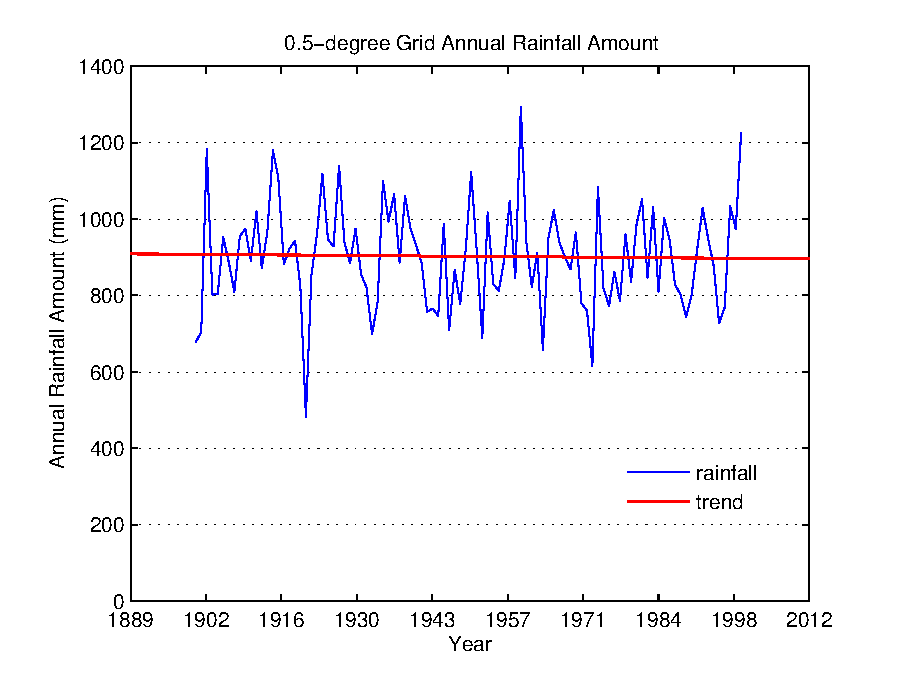
\includegraphics[width=0.7\textwidth]{./img/grid_annual_amount}
  \caption{Annual rainfall amount trend of monthly grid data}
  \label{fig:grid_annual_amount}
\end{figure}

There is no statistically significant trend in seasonal rainfall amounts
(Figure \ref{fig:grid_DJF_trend}).

\begin{figure}[htbp]
  \centering
    \subfloat[][DJF]{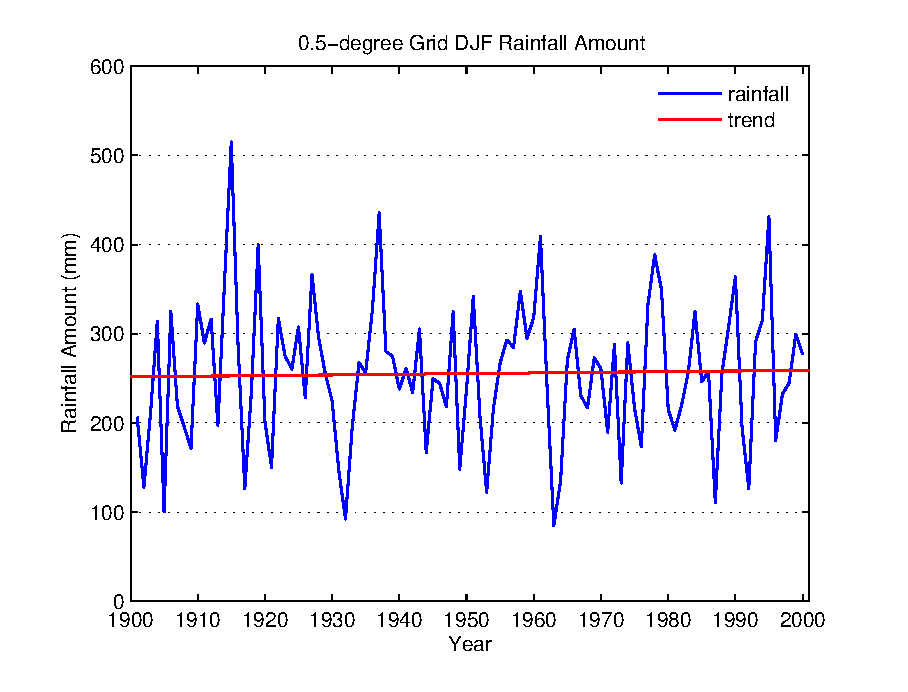
\includegraphics[width=0.5\textwidth]
{./img/grid_DJF_trend}}
    \subfloat[][MAM]{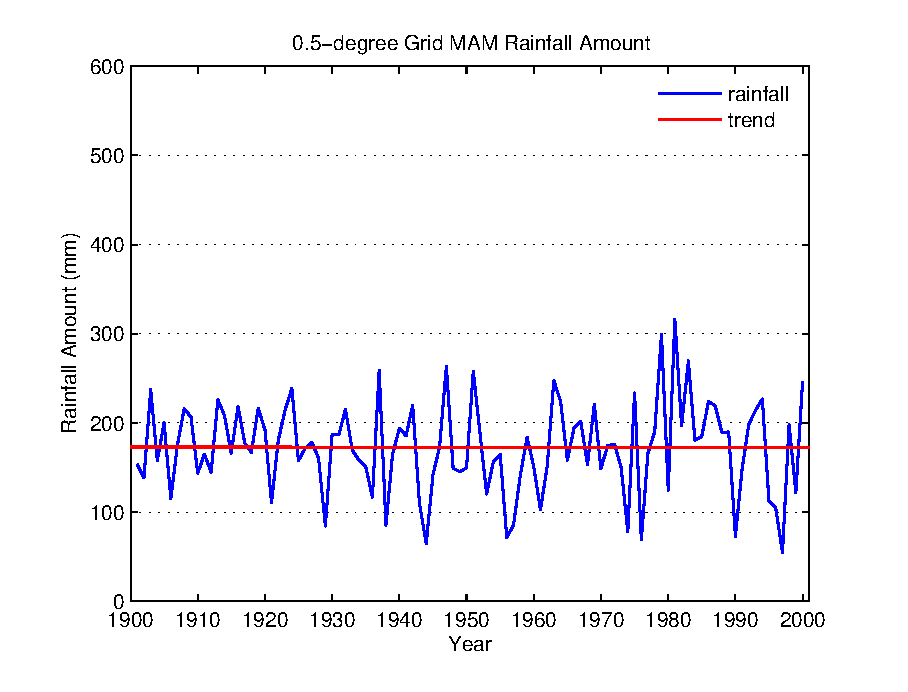
\includegraphics[width=0.5\textwidth]
{./img/grid_MAM_trend}}

    \subfloat[][JJA]{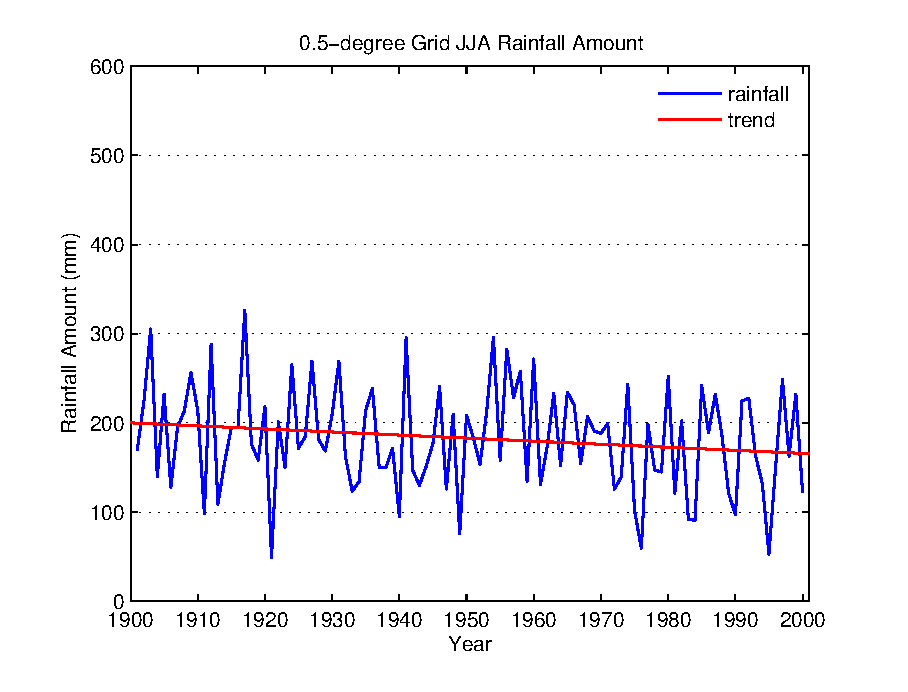
\includegraphics[width=0.5\textwidth]
{./img/grid_JJA_trend}}
    \subfloat[][SON]{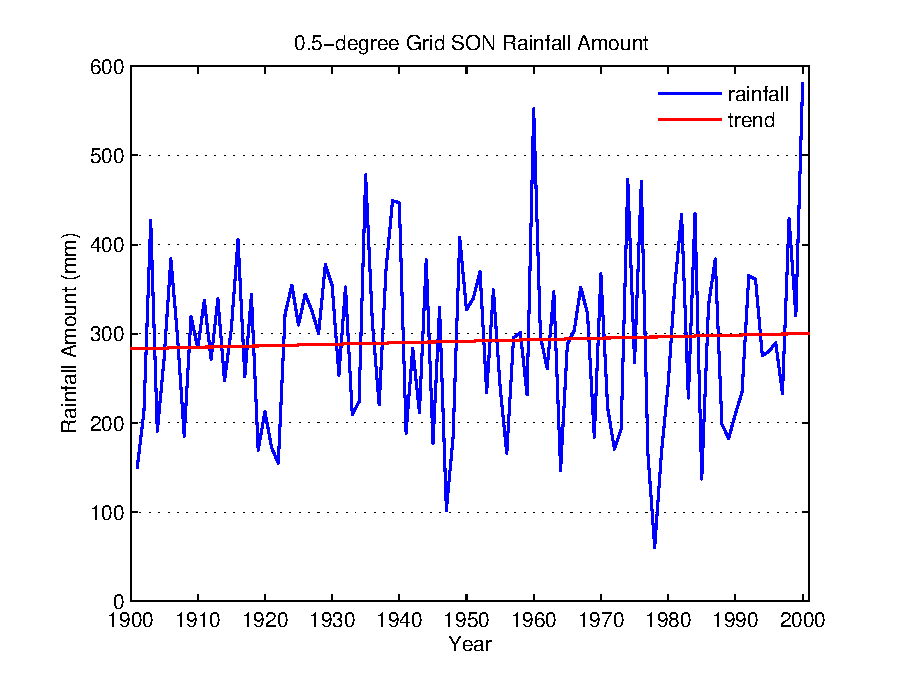
\includegraphics[width=0.5\textwidth]
{./img/grid_SON_trend}}
  \caption{Seasonal rainfall amount trend of monthly 0.5\textdegree\ grid
data}

  \label{fig:grid_DJF_trend}
\end{figure}

Monthly rainfall amount pattern shows more rainfall in autumn and winter months
with a peak in November, and less rainfall in spring and summer months (Figure
\ref{fig:grid_average_monthly}). Monthly analysis of the grid data shows more
detailed monthly trend in rainfall amount. Rainfall amounts in March show a
statistically significant ($p<0.05$) decreasing trend over 1981--2000 by both
simple linear regression and Mann-Kendall's test.

\begin{figure}[htbp]
  \centering
    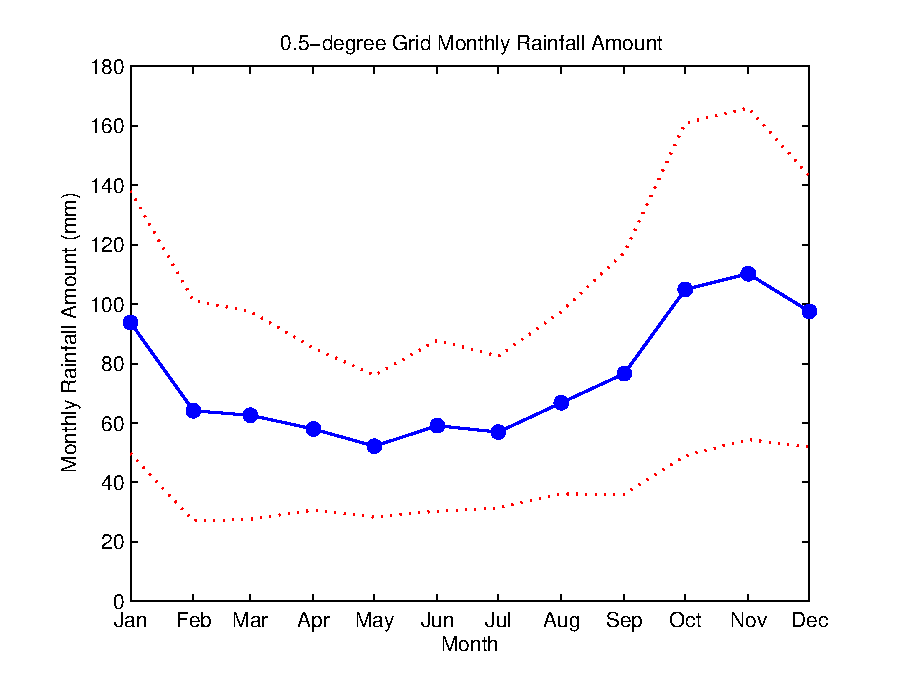
\includegraphics[width=0.7\textwidth]{./img/grid_average_monthly}
  \caption[Average monthly rainfall patterns of monthly grid data]{Average
monthly rainfall patterns of monthly grid data. Dotted lines indicate standard
deviation with 95\% confidence level.}
  \label{fig:grid_average_monthly}
\end{figure}

Rainfall amounts in July have a decreasing trend throughout the whole data
period (1901--2000) (Figure \ref{fig:grid_july_trend}).

\begin{figure}
  \centering
    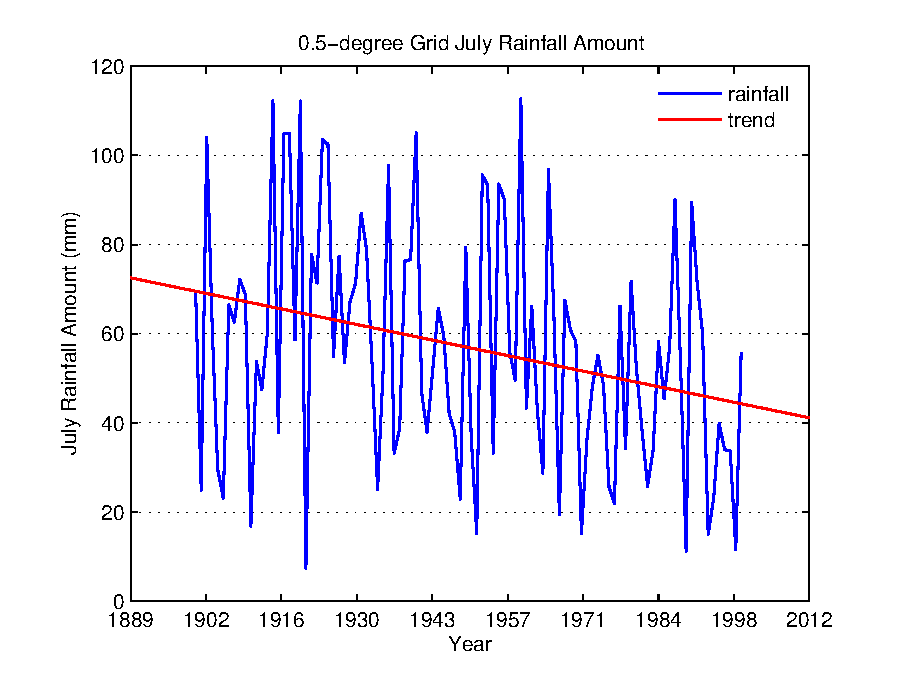
\includegraphics[width=0.7\textwidth]{./img/grid_july_trend}
  \caption{July rainfall amount trend over 1901-2000}
  \label{fig:grid_july_trend}
\end{figure}

%%%%%%%%%%%%%%%%%%%%%%%%%%%%%%%%%%%%%%%%%%%%%%%%%%%%%%%%%%
\section{Daily Precipitation}
\label{sec:DailyRainfallStationData}

Annual rainfall amount from Poverty Bottom (PB), Friston Tower (FT), Eastbourne
Wilmington (EW), Litlington (LI) and Seaford D. Road (SDR) stations are
significantly different from those of Plumpton (PL) or High Park Farm (HPF), for
example. This may be because of the distance from each other (see Figure
\ref{fig:DailyRainfallDataSite}) although all stations are placed in the
0.5\textdegree\ grid square.

%By stations, compare annual and monthly trend of rainfall amount and SDII.
%first of all, compare amounts for the Grid data. do this for annual and
%monthly. Are there July decrease and September increase in daily data too?
%if found and yes, it can be argued that SDII trends found in station daily
%data may be ture for the Grid Data.

\paragraph{Rainfall Amount (RR)}
\label{sec:RainfallAmountRR}

All the station show no statistically significant trend in annual rainfall
amount. This result agrees with that of monthly 0.5\textdegree\ grid rainfall
data.

For all the stations except Ditchling Road (DR), High Park Farm (HPF) and
Housedean (HD), monthly rainfall amount in March showed statistically
significant downward trends over the last two decades. The similar downward
trends are observed with rainfall amounts in July for the last decades with the
exception of DR, PB, HPF and HD stations. For longer periods, the trend of
monthly rainfall amount is inconclusive. This broadly agrees with the results
from the 0.5\textdegree\ grid data analysis. For monthly 0.5\textdegree\ grid
data, July months showed a decrease in rainfall amount.

\begin{figure}[htbp]
  \centering
  \subfloat[DR]{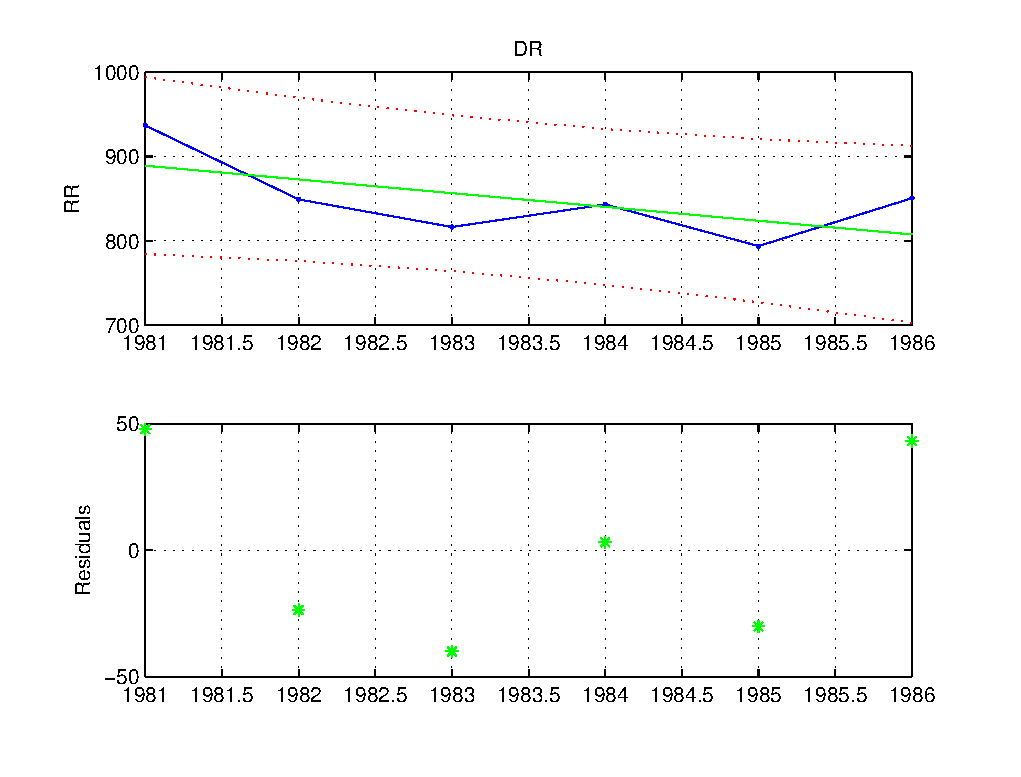
\includegraphics[width=0.33\textwidth]{./img/dr_rr}}
  \subfloat[SO]{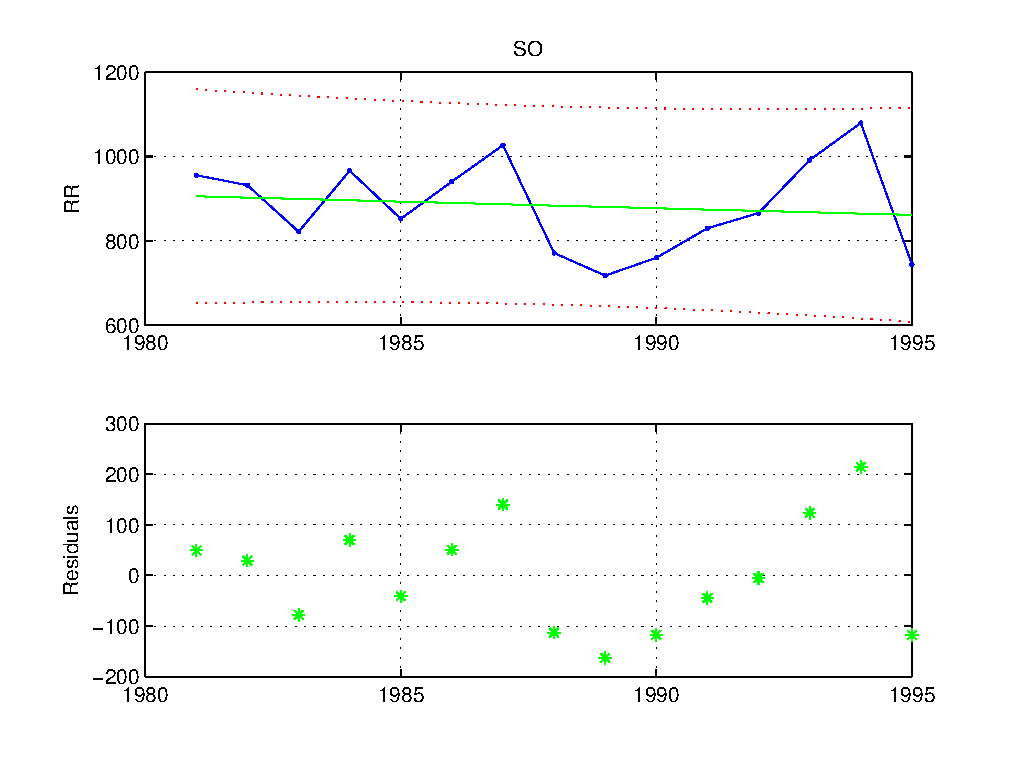
\includegraphics[width=0.33\textwidth]{./img/so_rr}}
  \subfloat[PL]{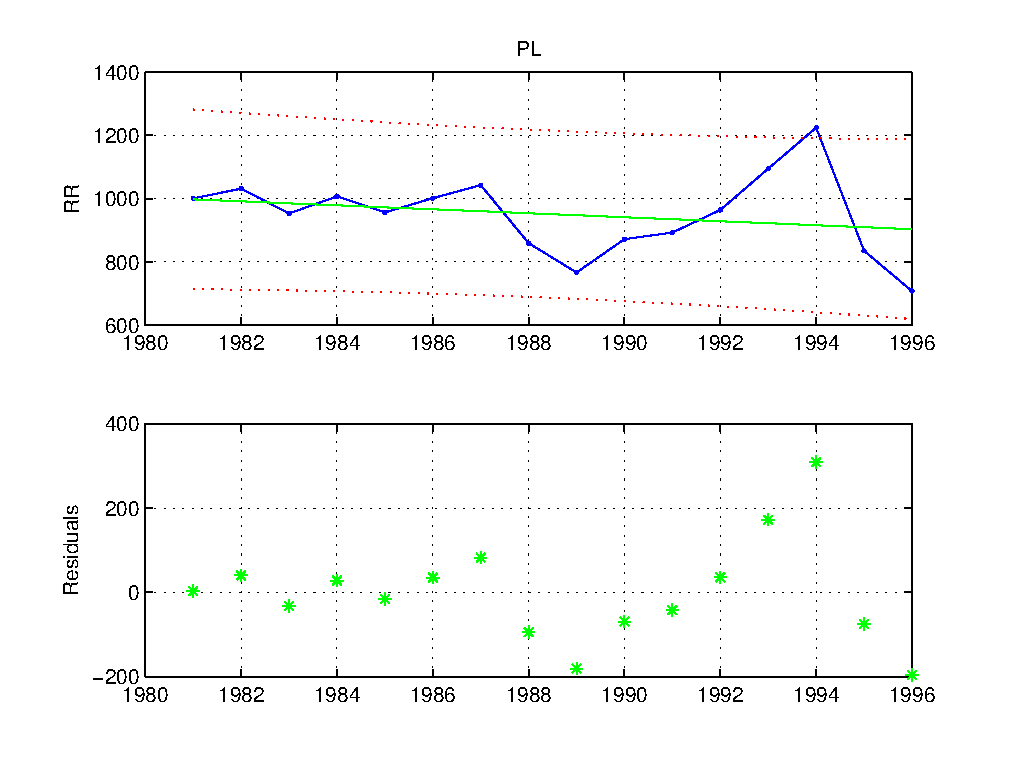
\includegraphics[width=0.33\textwidth]{./img/pl_rr}}

  \subfloat[PB]{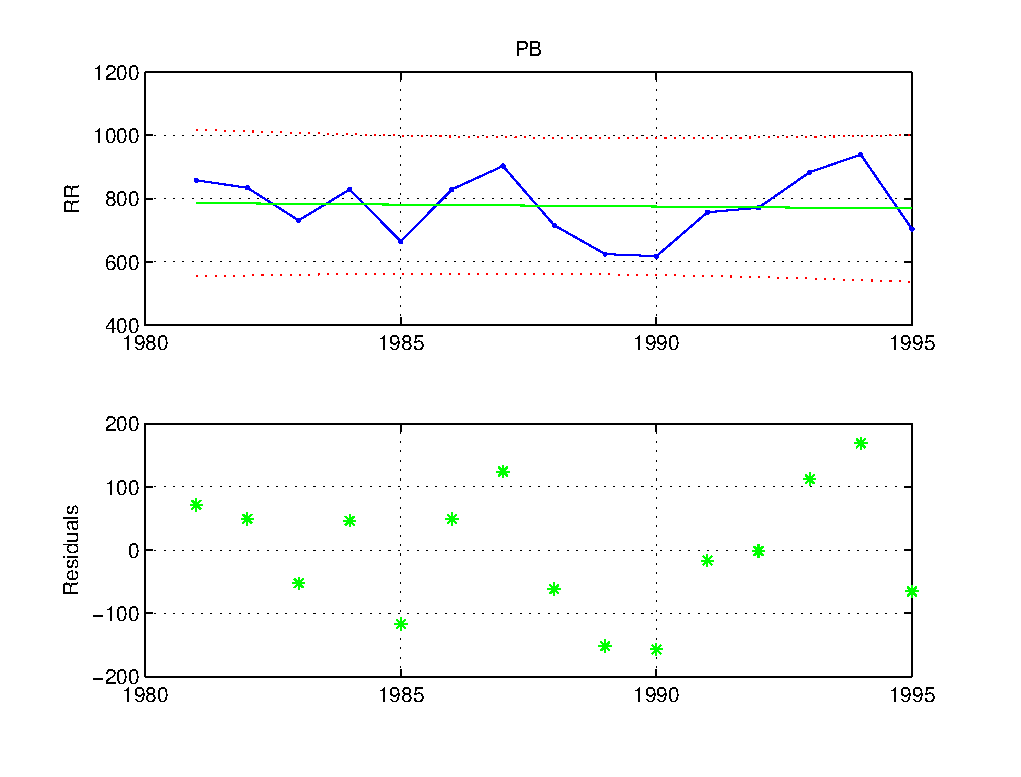
\includegraphics[width=0.33\textwidth]{./img/pb_rr}}
  \subfloat[SDR]{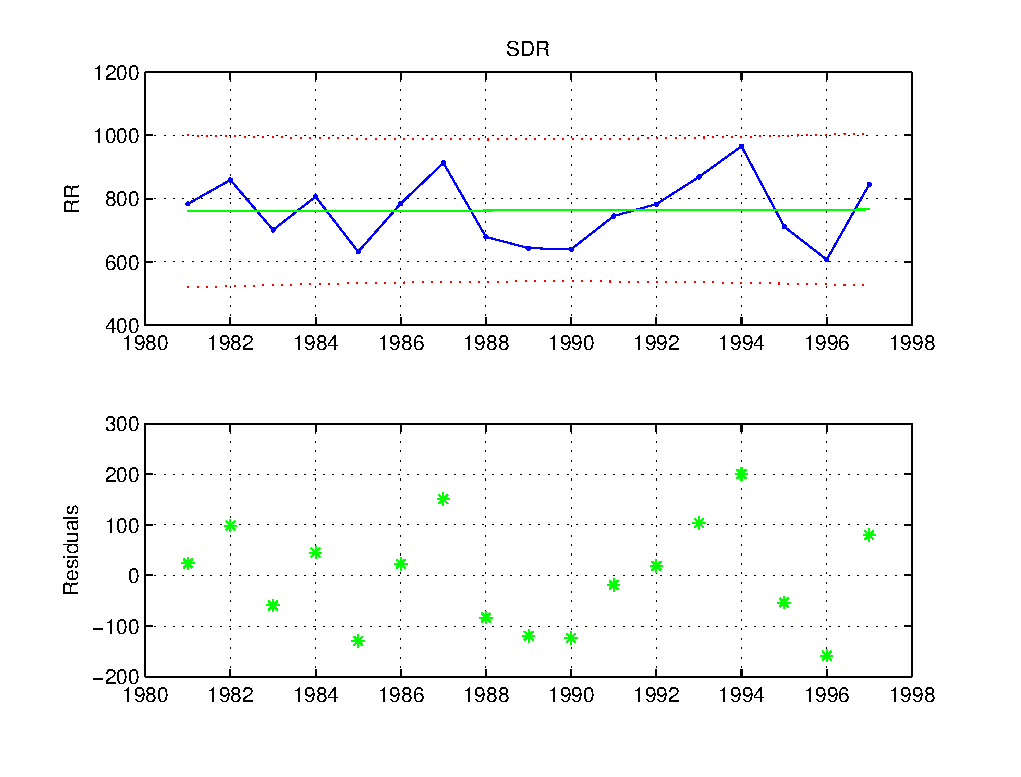
\includegraphics[width=0.33\textwidth]{./img/sdr_rr}}
  \subfloat[EW]{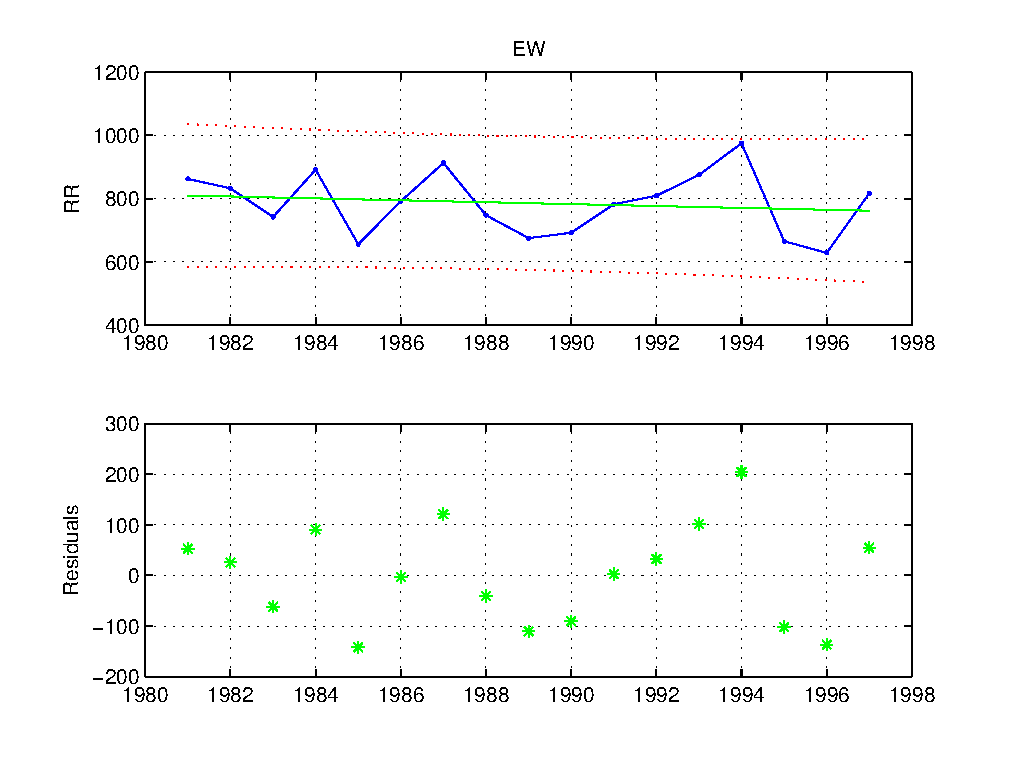
\includegraphics[width=0.33\textwidth]{./img/ew_rr}}

  \subfloat[FT]{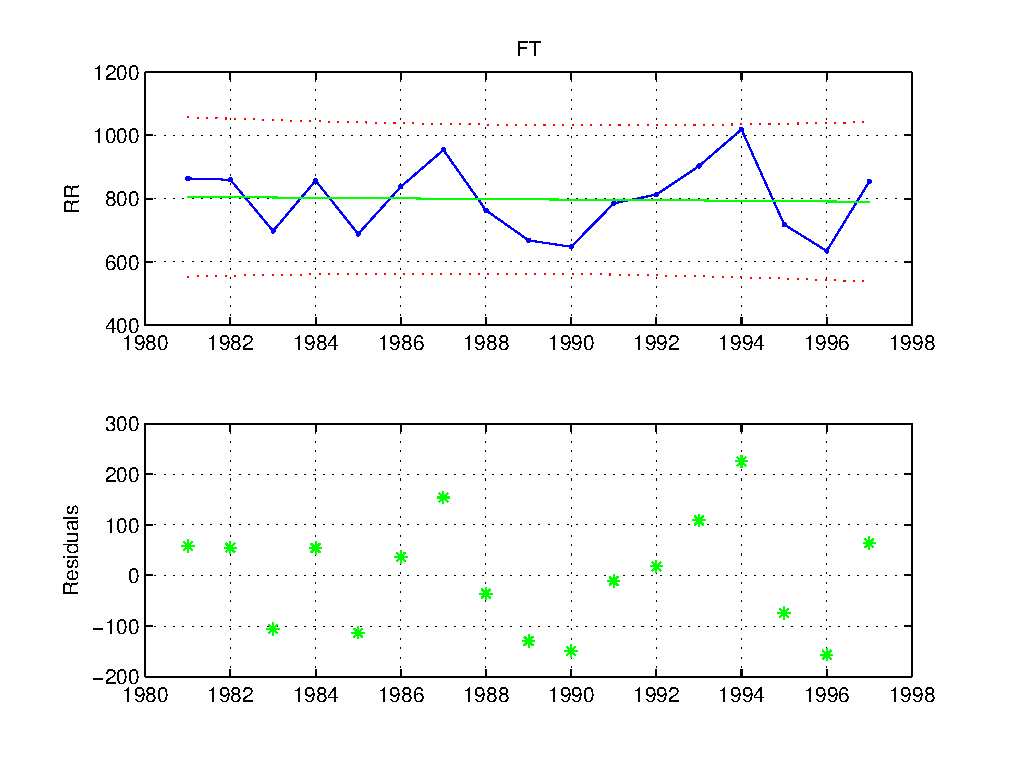
\includegraphics[width=0.33\textwidth]{./img/ft_rr}}
  \subfloat[LI]{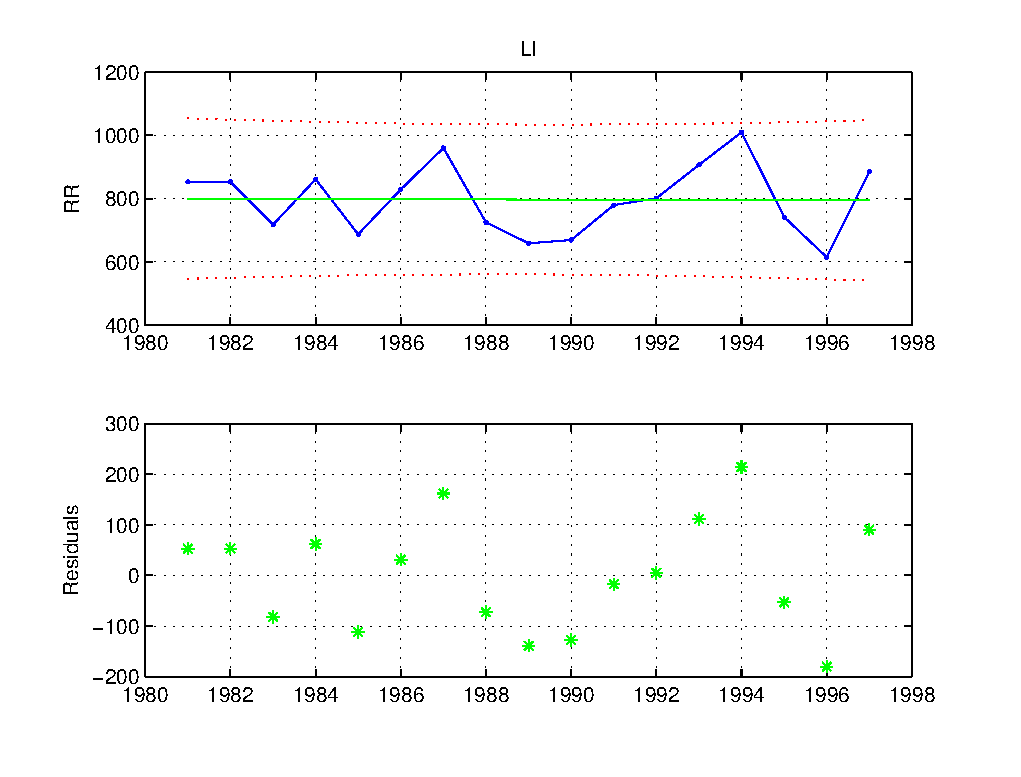
\includegraphics[width=0.33\textwidth]{./img/li_rr}}
  \subfloat[HPF]{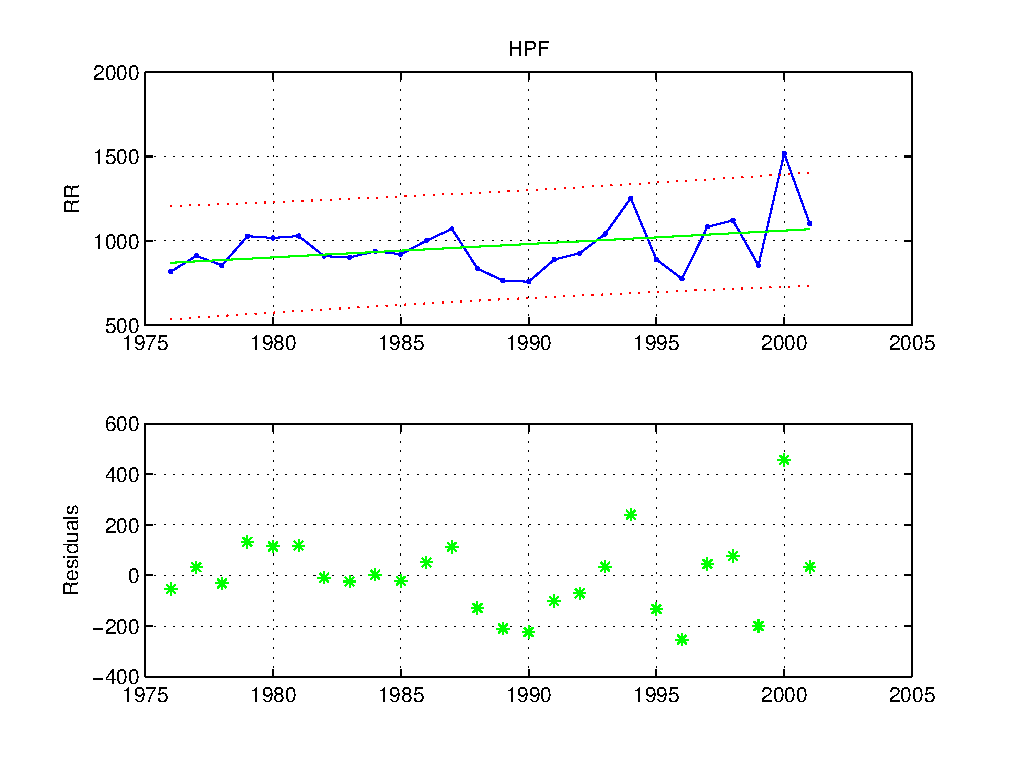
\includegraphics[width=0.33\textwidth]{./img/hpf_rr}}

  \subfloat[HD]{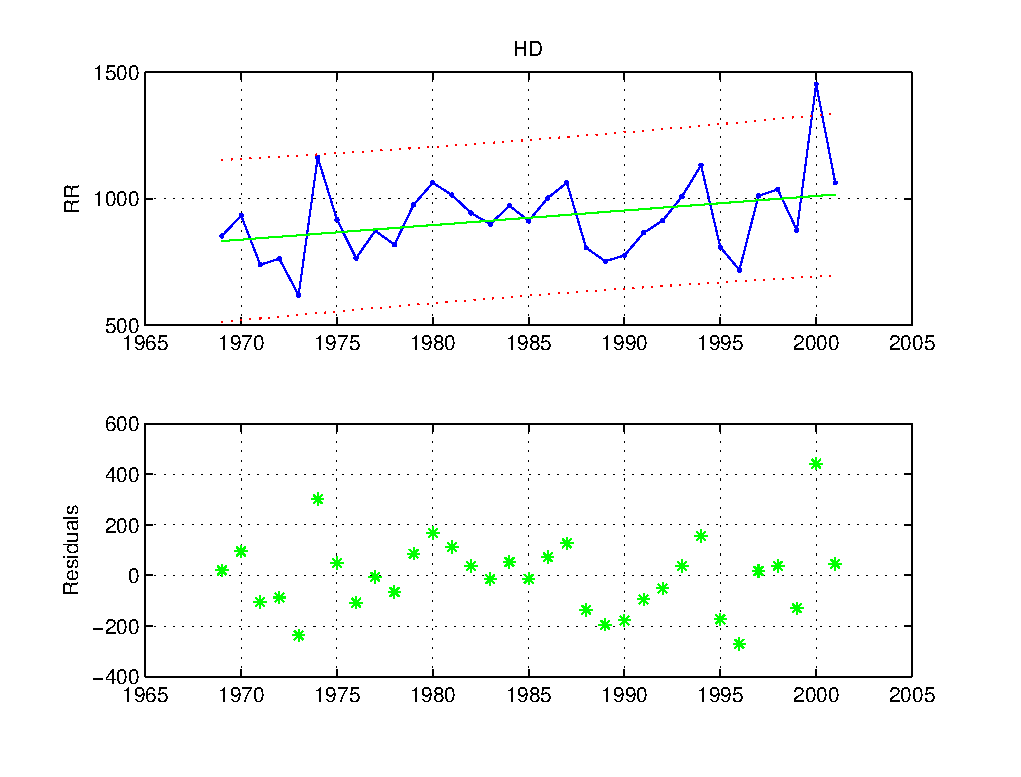
\includegraphics[width=0.33\textwidth]{./img/hd_rr}}
  \subfloat[FF]{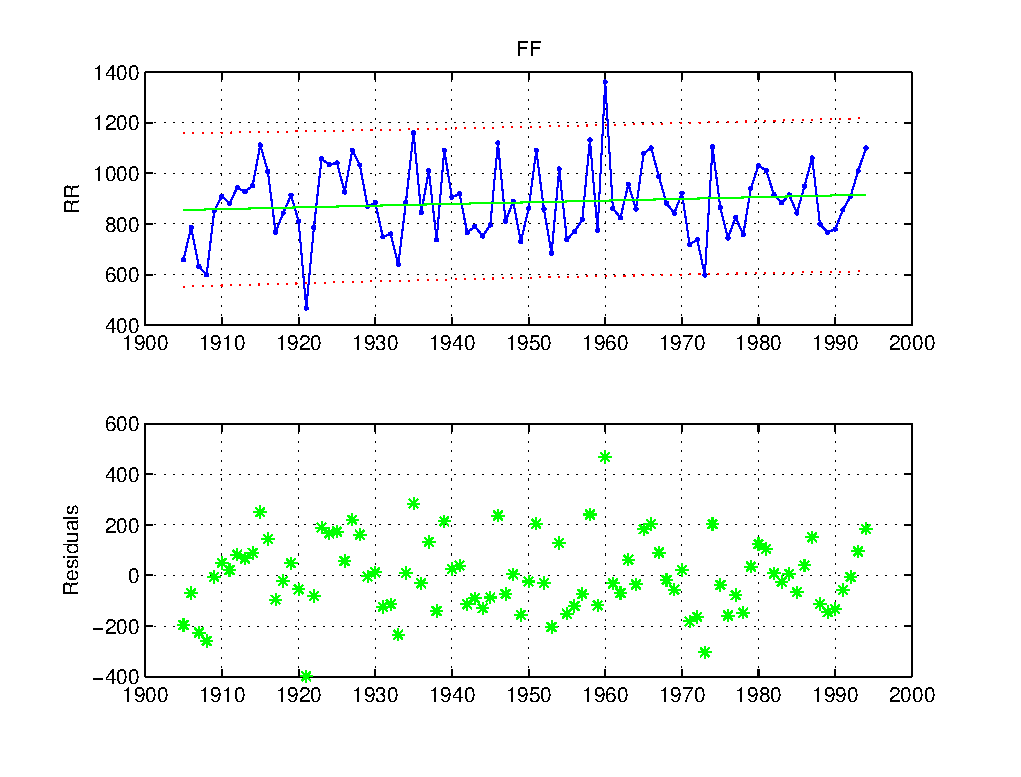
\includegraphics[width=0.33\textwidth]{./img/ff_rr}}
  \caption{Trends of annual rainfall amount (RR) at daily data stations}
  \label{fig:FF_annual_RR}
\end{figure}

\paragraph{Number of Wet Days (RR1)}
\label{sec:NumberOfRaindaysRR1}

The number of wet days per year decreased at PL and FF stations (M-K, $p<0.05$)
(Figure \ref{fig:FF_annual_RR1}). Although not all the stations showed
statistically significant annual trends, the ones with significant annual trend
in the number of wet days show downward trends in the number of wet days over
the data periods.
%A downward annual trend was also confirmed by Mann-Kendall test ($p<0.05$) for
%the same periods.

The month of March shows significant decreasing trends in the number of wet days
per month over 1980--1999. The month of July also shows decreasing trend in the
recent decade.

\begin{figure}[htbp]
  \centering
  \subfloat[DR]{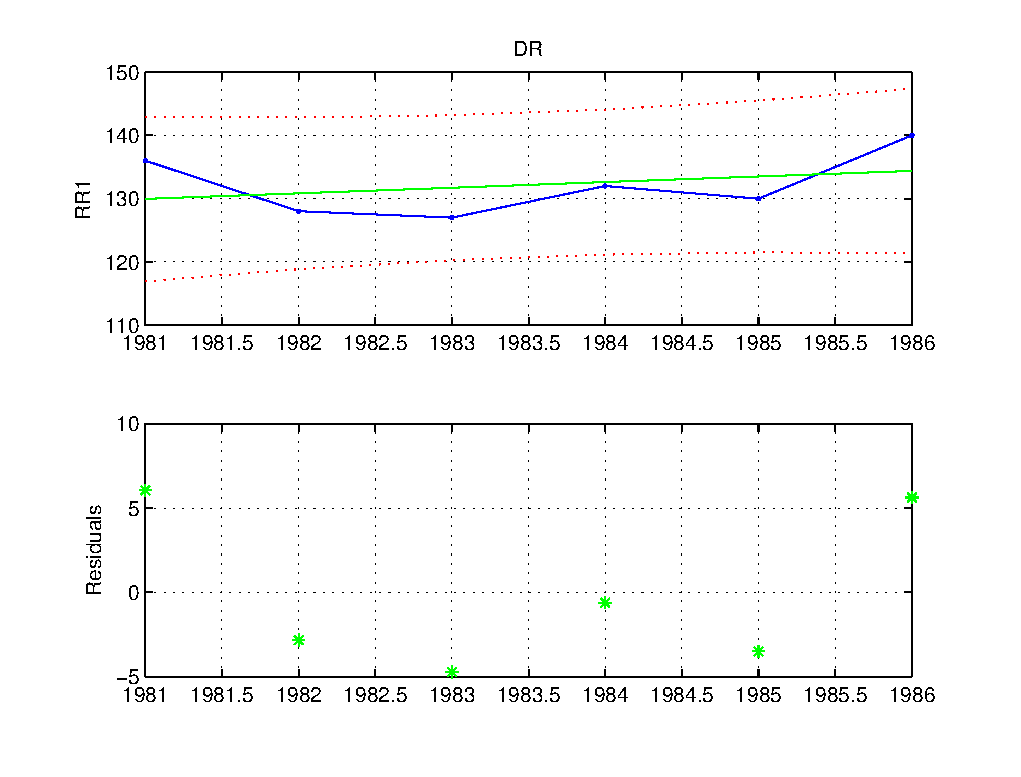
\includegraphics[width=0.33\textwidth]{./img/dr_rr1}}
  \subfloat[SO]{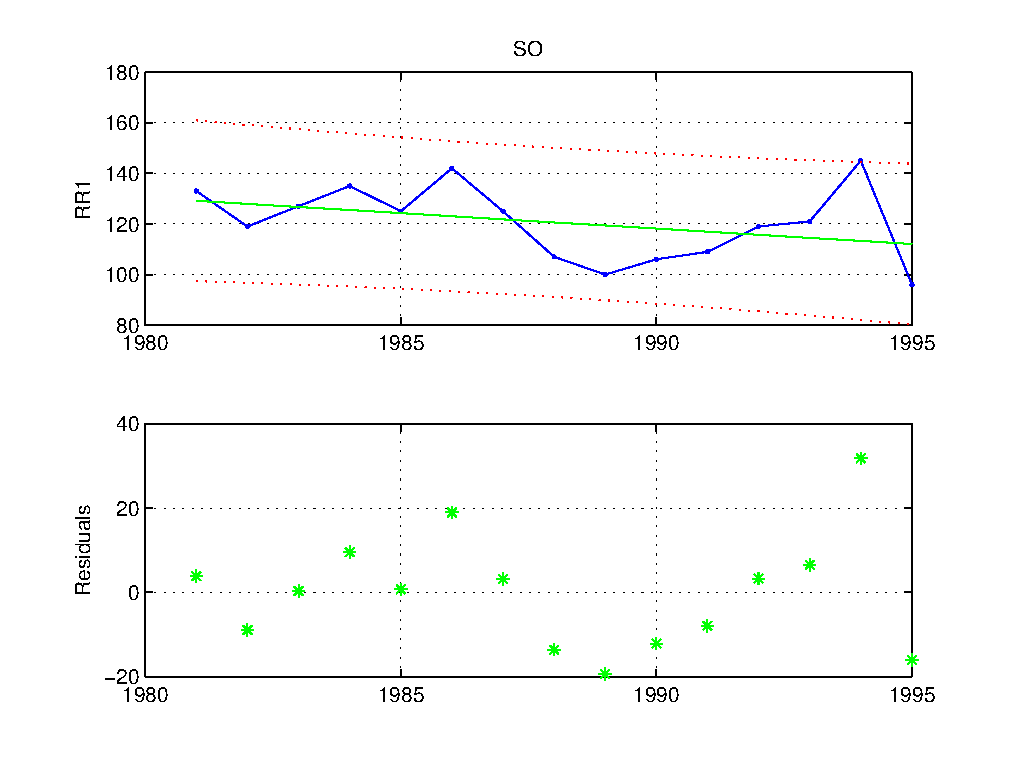
\includegraphics[width=0.33\textwidth]{./img/so_rr1}}
  \subfloat[PL]{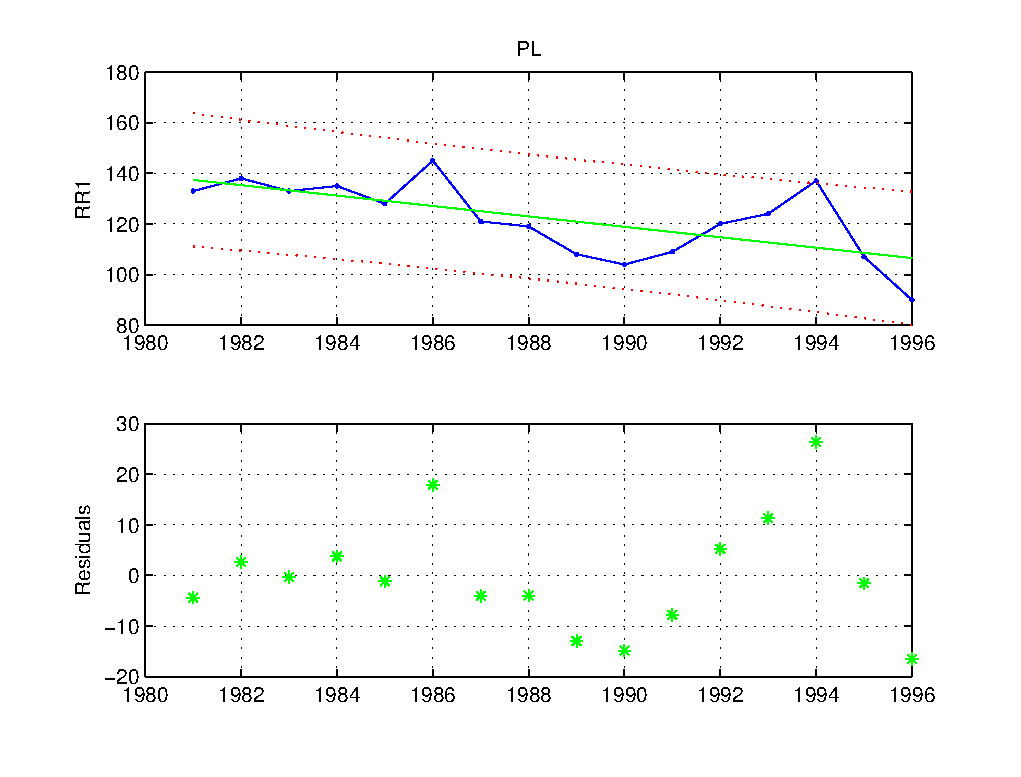
\includegraphics[width=0.33\textwidth]{./img/pl_rr1}}

  \subfloat[PB]{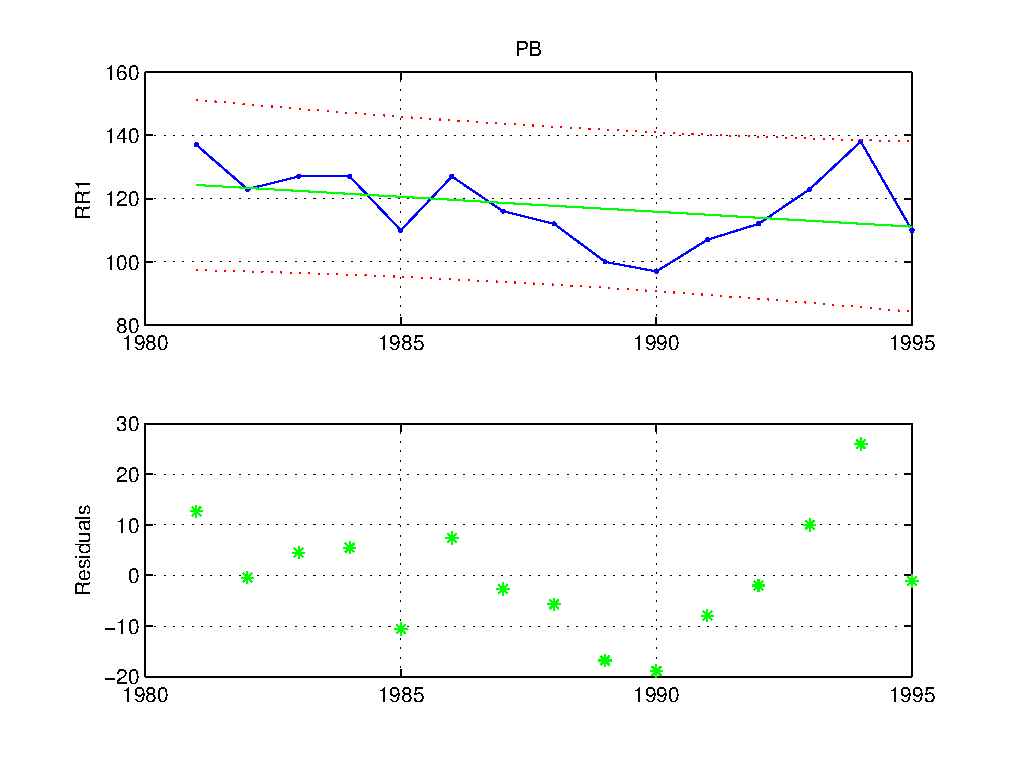
\includegraphics[width=0.33\textwidth]{./img/pb_rr1}}
  \subfloat[SDR]{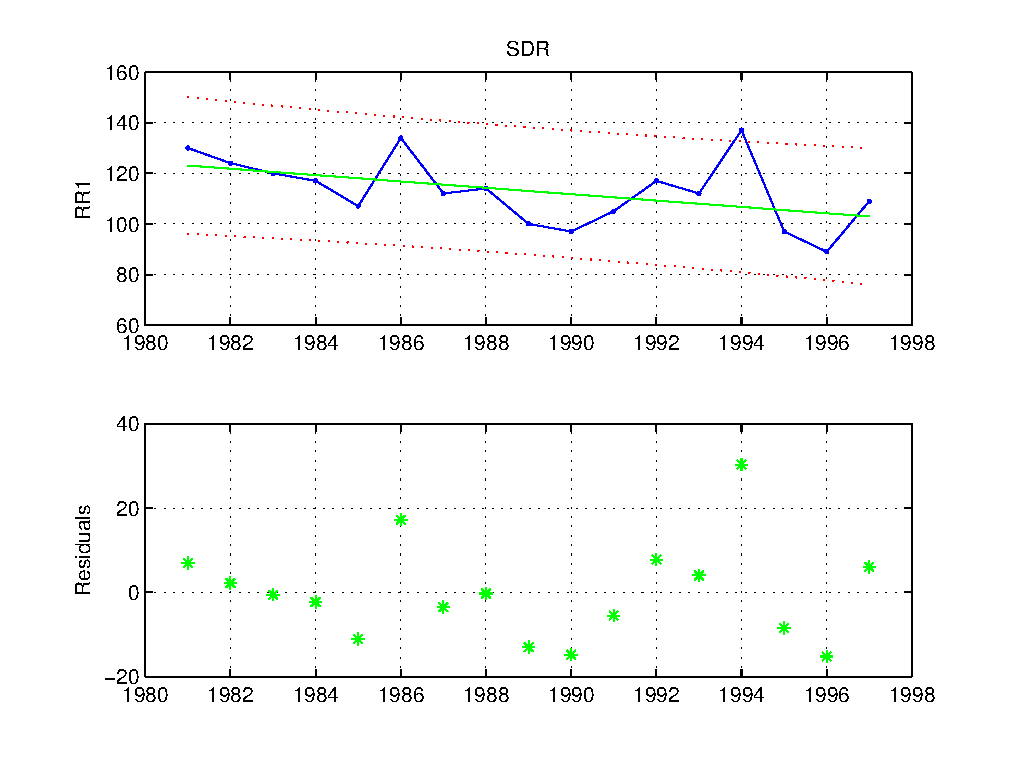
\includegraphics[width=0.33\textwidth]{./img/sdr_rr1}}
  \subfloat[EW]{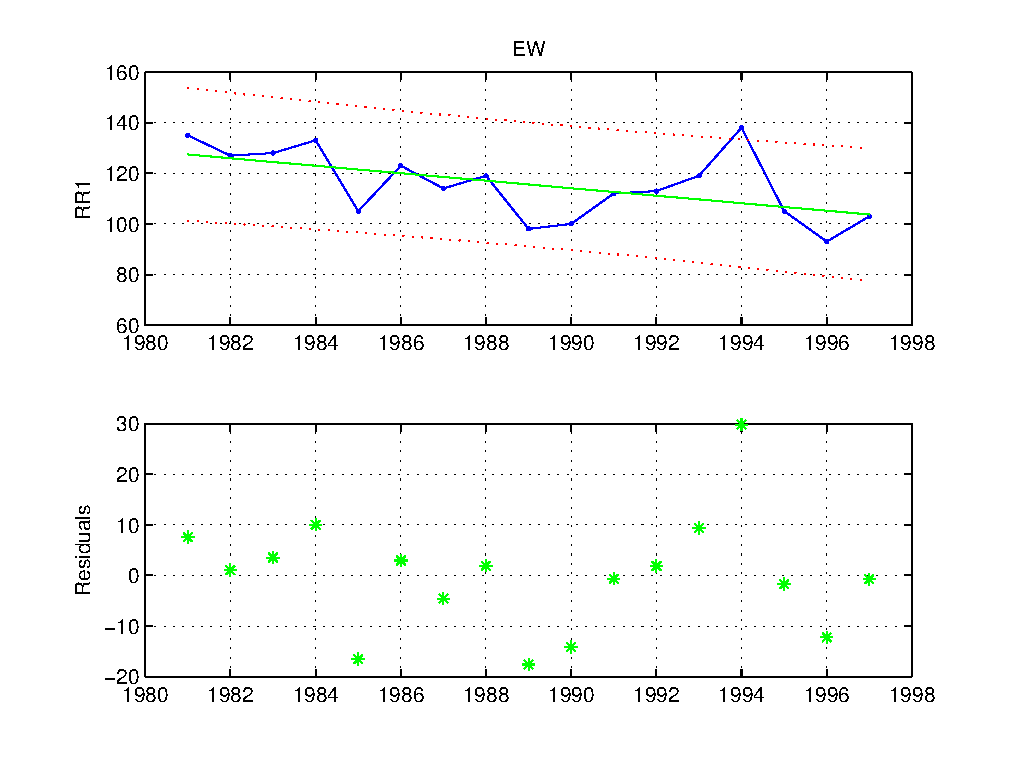
\includegraphics[width=0.33\textwidth]{./img/ew_rr1}}

  \subfloat[FT]{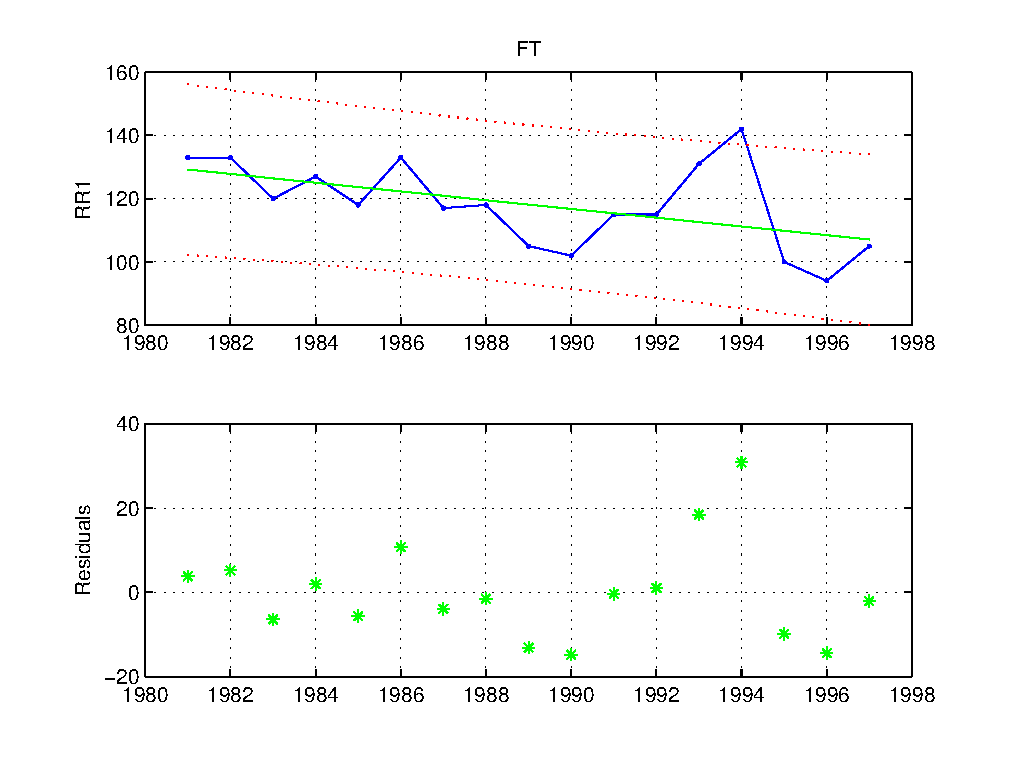
\includegraphics[width=0.33\textwidth]{./img/ft_rr1}}
  \subfloat[LI]{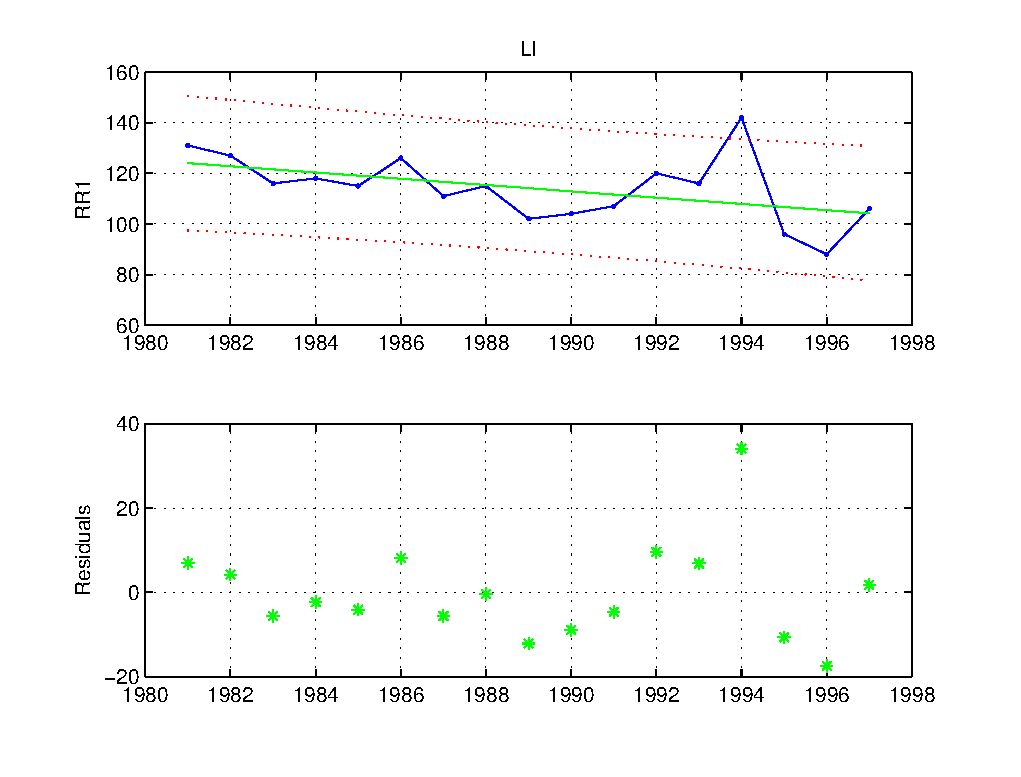
\includegraphics[width=0.33\textwidth]{./img/li_rr1}}
  \subfloat[HPF]{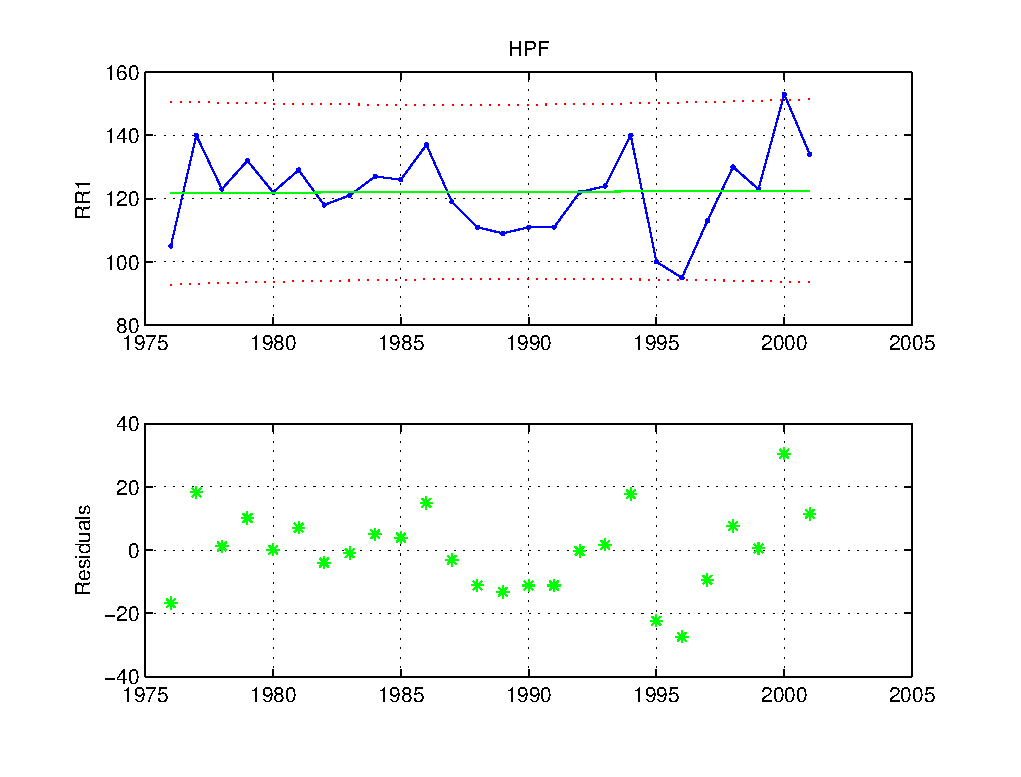
\includegraphics[width=0.33\textwidth]{./img/hpf_rr1}}

  \subfloat[HD]{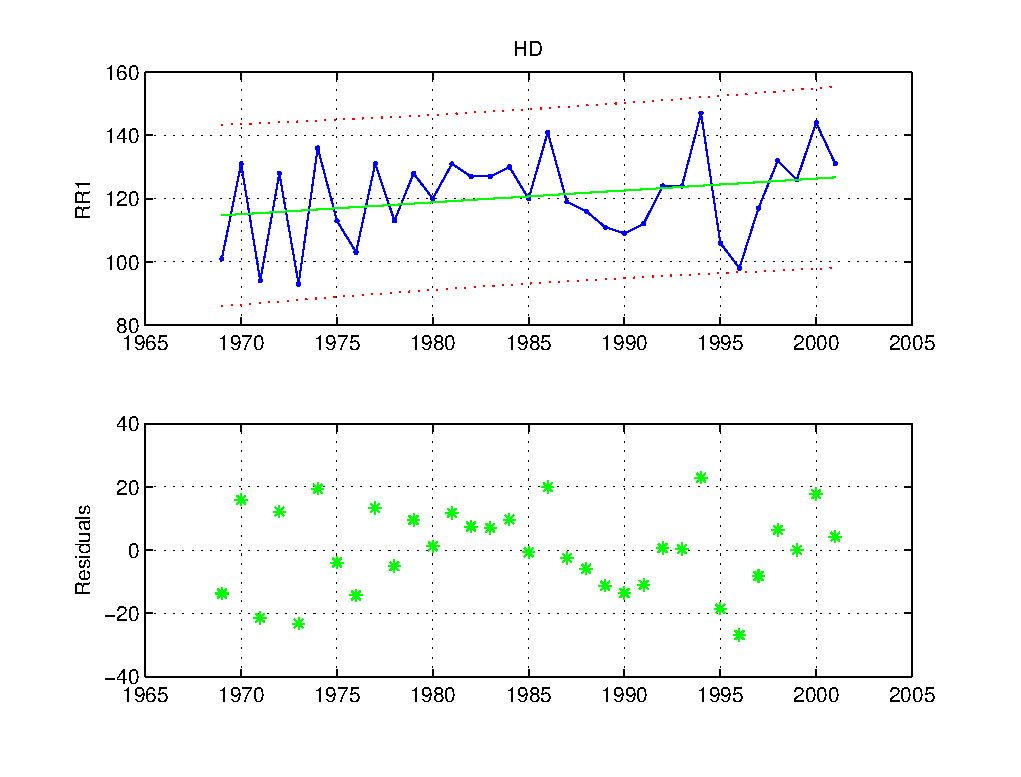
\includegraphics[width=0.33\textwidth]{./img/hd_rr1}}
  \subfloat[FF]{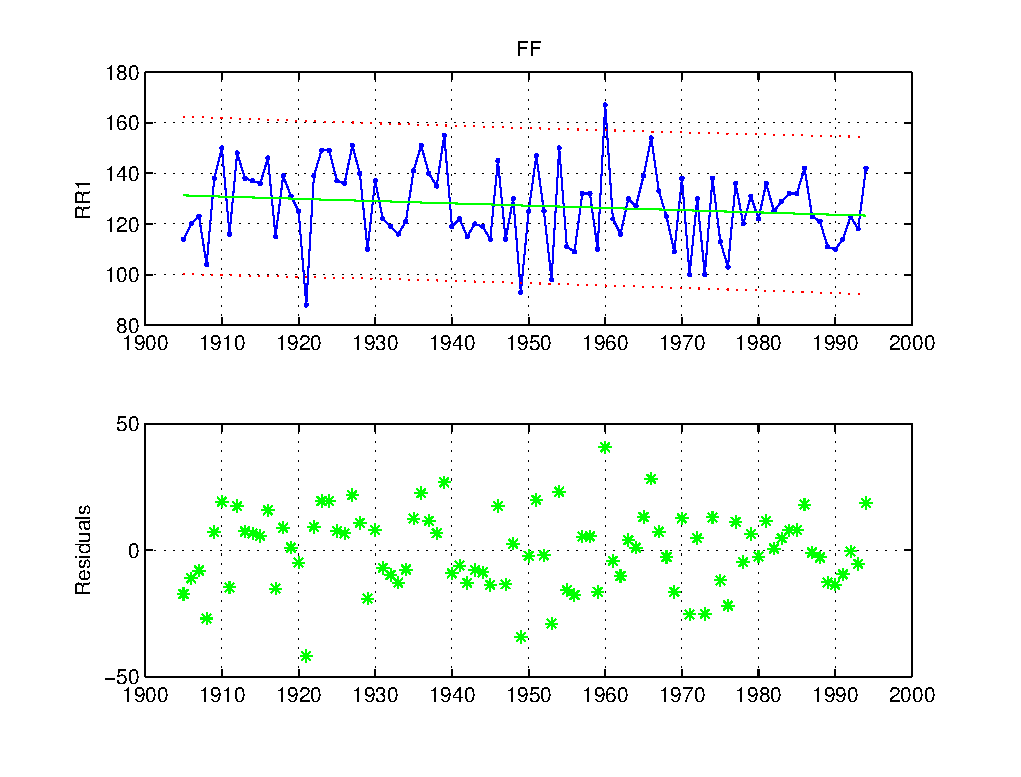
\includegraphics[width=0.33\textwidth]{./img/ff_rr1}}
  \caption{Trends of number of wetdays (RR1) at daily data stations}
  \label{fig:FF_annual_RR1}
\end{figure}

\paragraph{Simple Daily Intensity Index (SDII)}
\label{sec:SimpleDailyIntensityIndex}
As expected, PL \& FF again showed a significant annual trend in SDII. The rest
of the stations showed no significant results. FF station showed upward annual
trends in SDII throughout the data periods (Figure \ref{fig:FF_annual_SDII}).
All the cases with significant trends exhibited increasing trend of annual
SDII.

\begin{figure}[htbp]
  \centering
  \subfloat[DR]{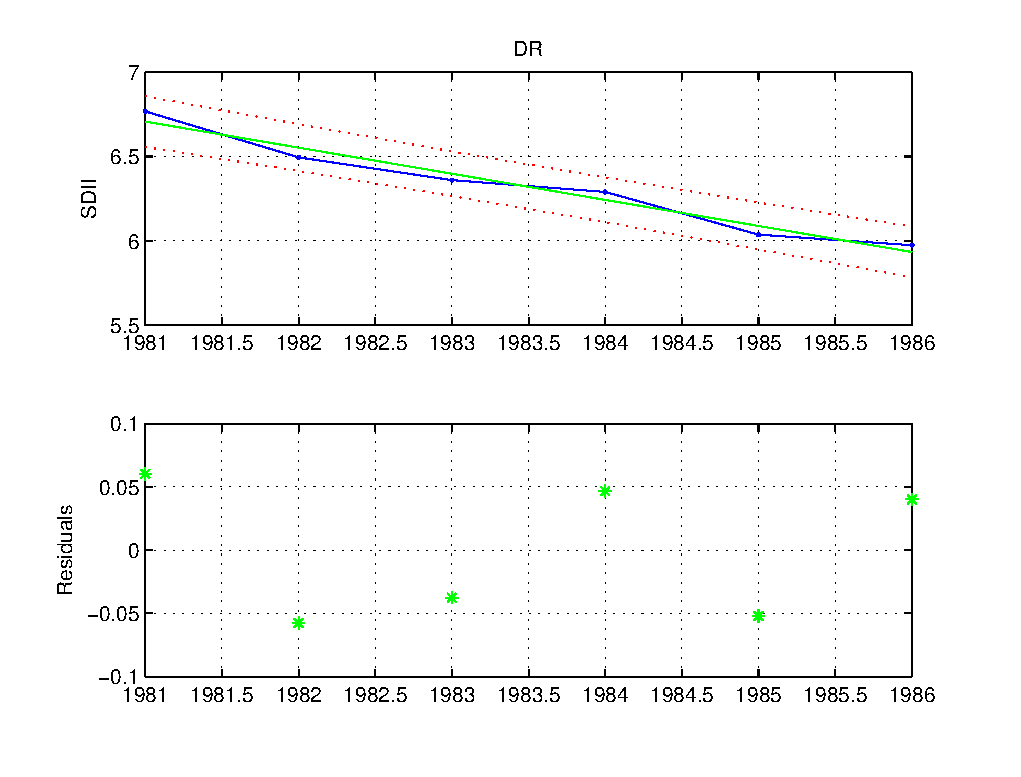
\includegraphics[width=0.33\textwidth]{./img/dr_sdii}}
  \subfloat[SO]{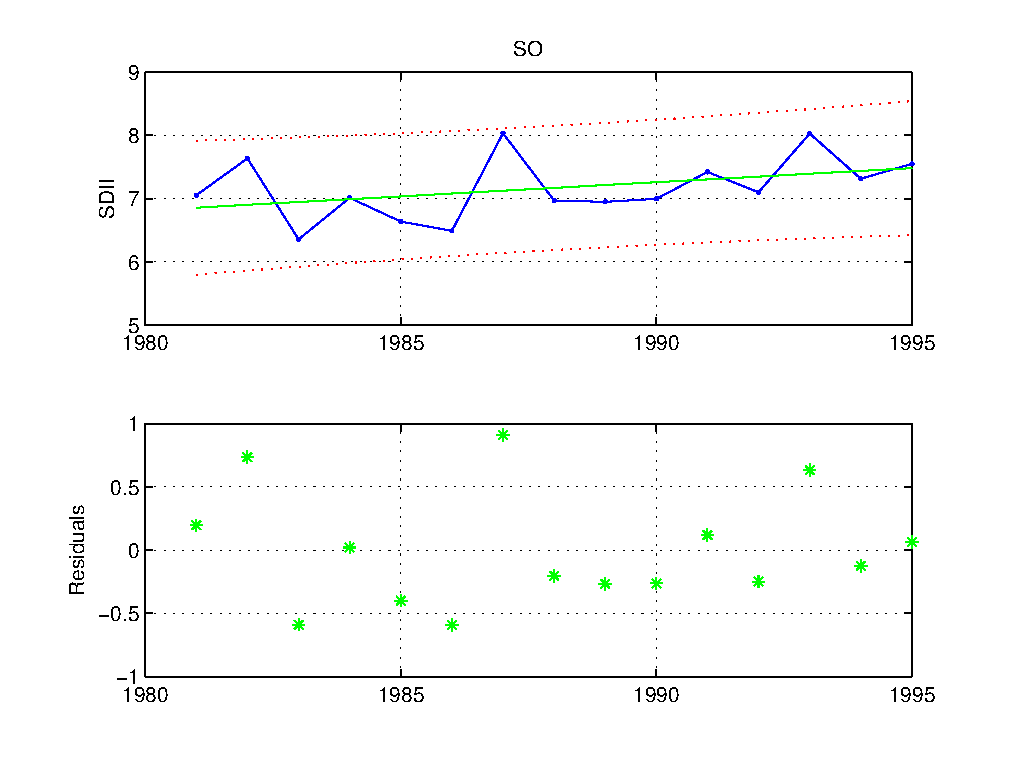
\includegraphics[width=0.33\textwidth]{./img/so_sdii}}
  \subfloat[PL]{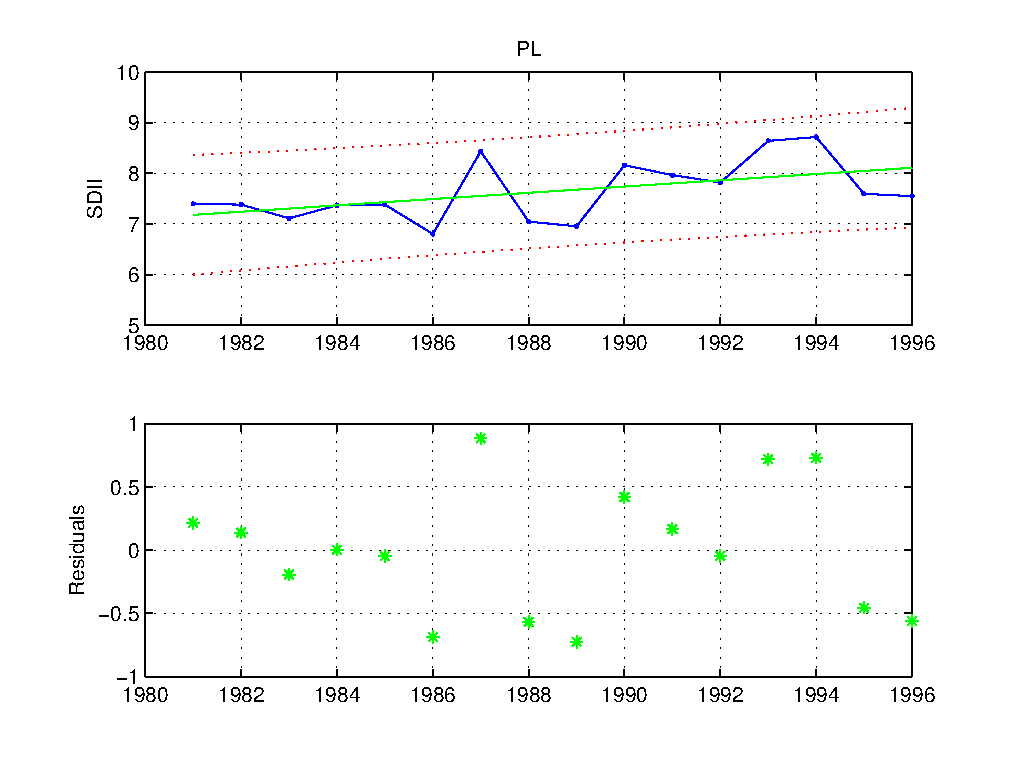
\includegraphics[width=0.33\textwidth]{./img/pl_sdii}}

  \subfloat[PB]{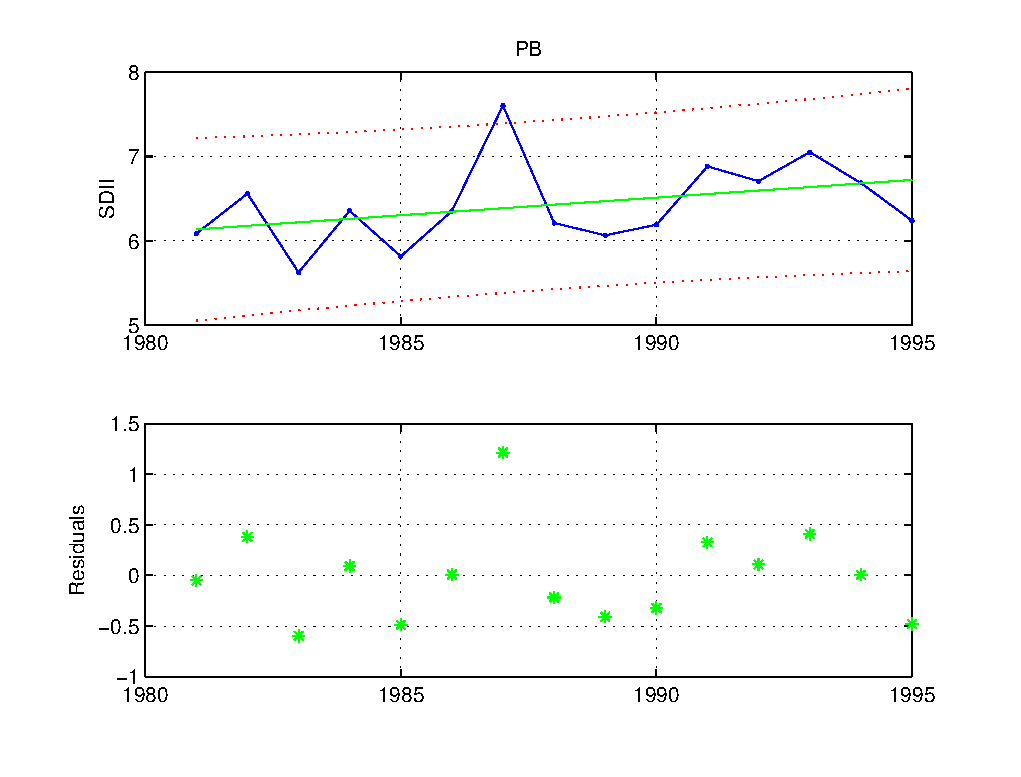
\includegraphics[width=0.33\textwidth]{./img/pb_sdii}}
  \subfloat[SDR]{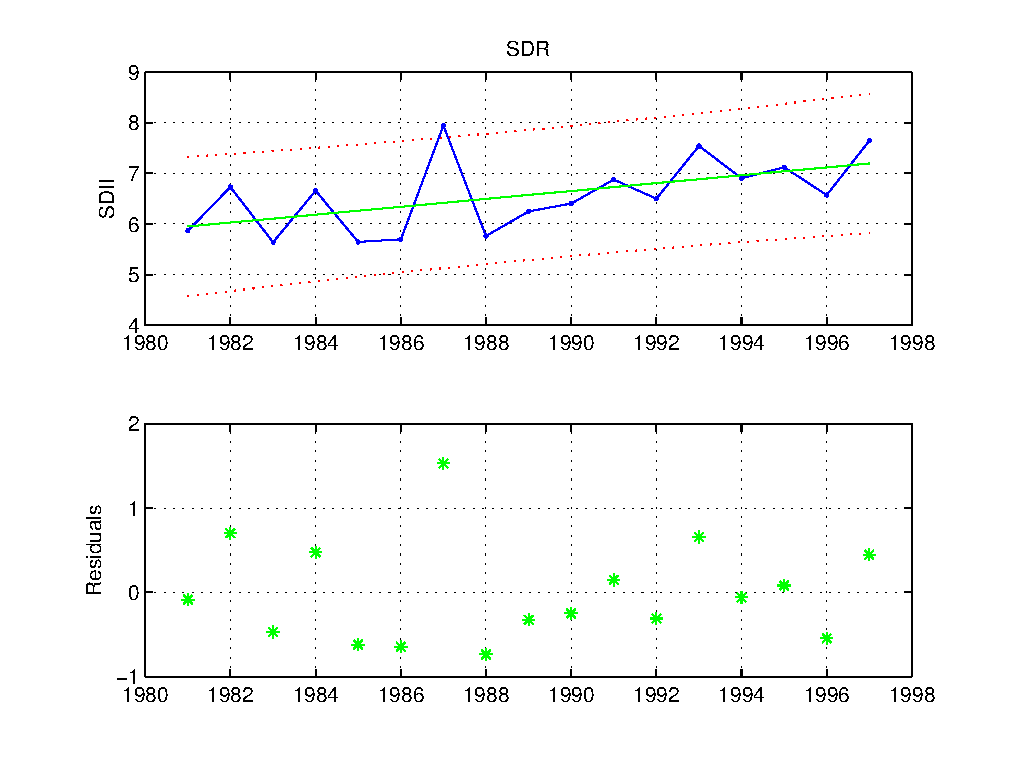
\includegraphics[width=0.33\textwidth]{./img/sdr_sdii}}
  \subfloat[EW]{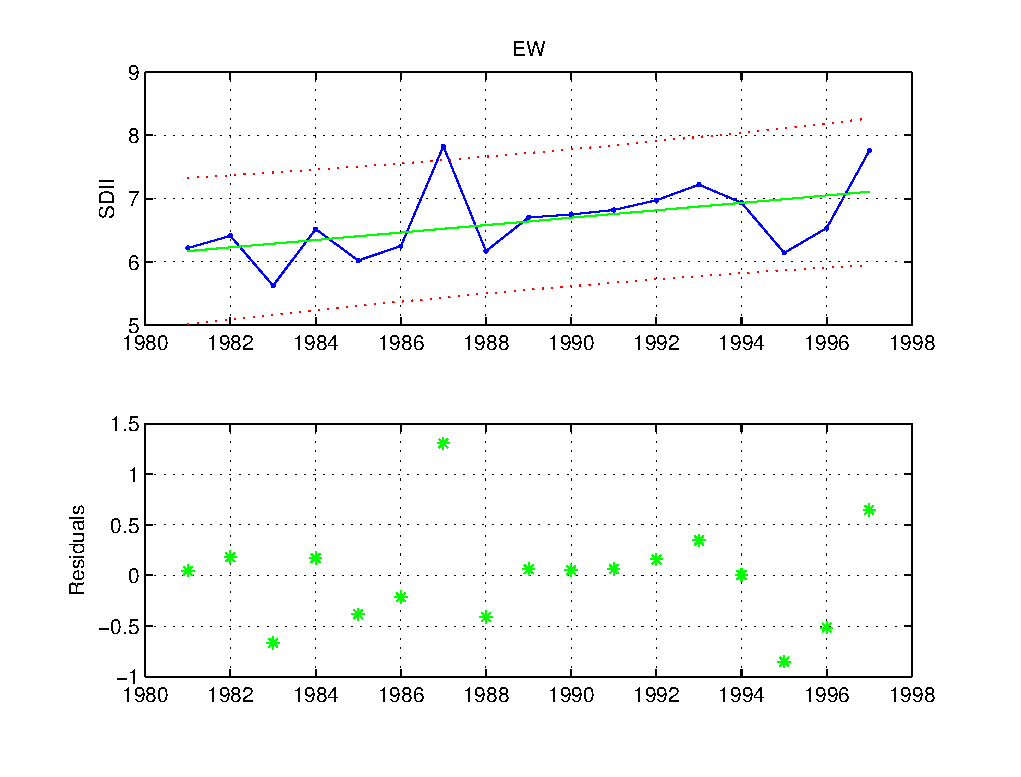
\includegraphics[width=0.33\textwidth]{./img/ew_sdii}}

  \subfloat[FT]{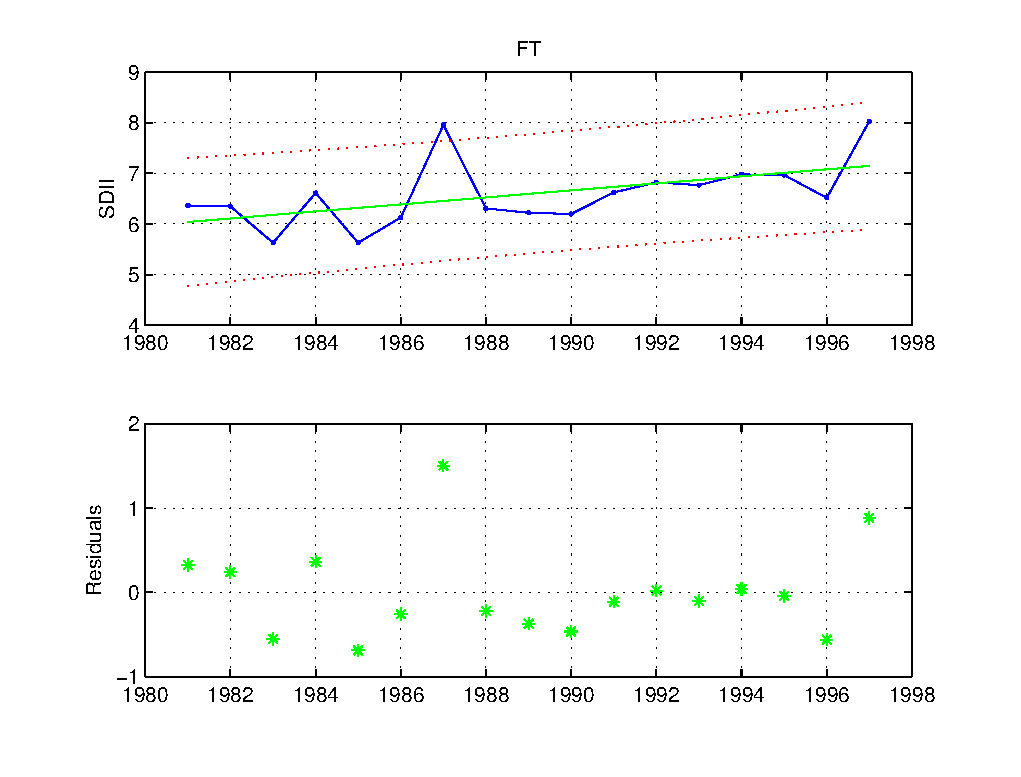
\includegraphics[width=0.33\textwidth]{./img/ft_sdii}}
  \subfloat[LI]{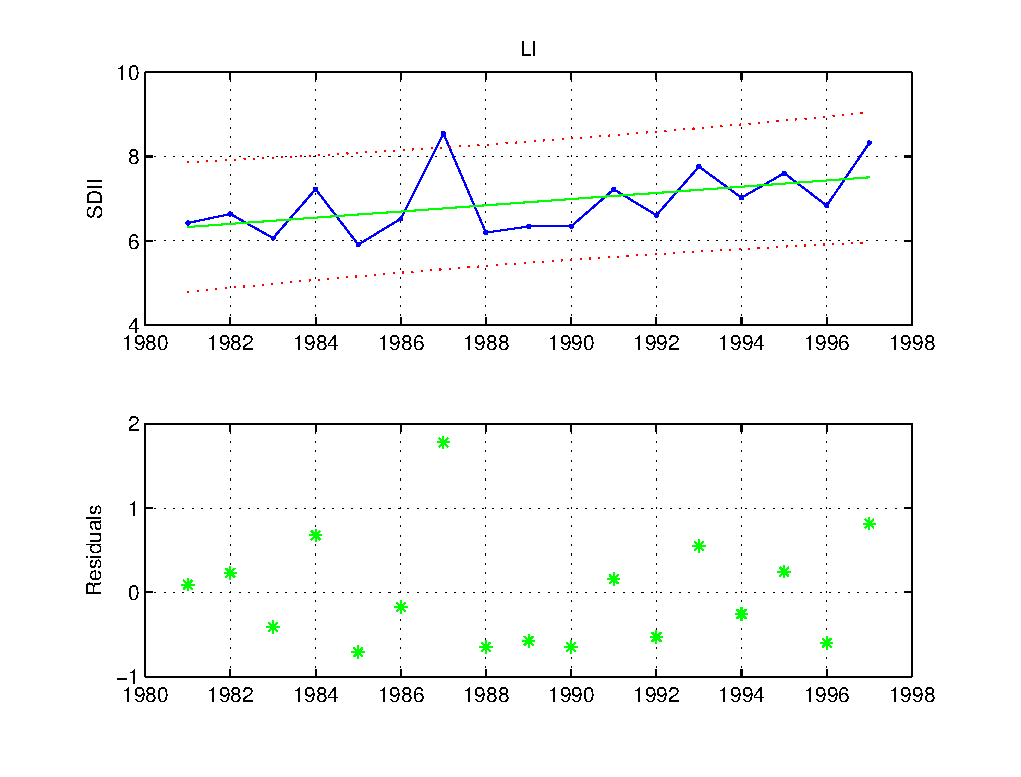
\includegraphics[width=0.33\textwidth]{./img/li_sdii}}
  \subfloat[HPF]{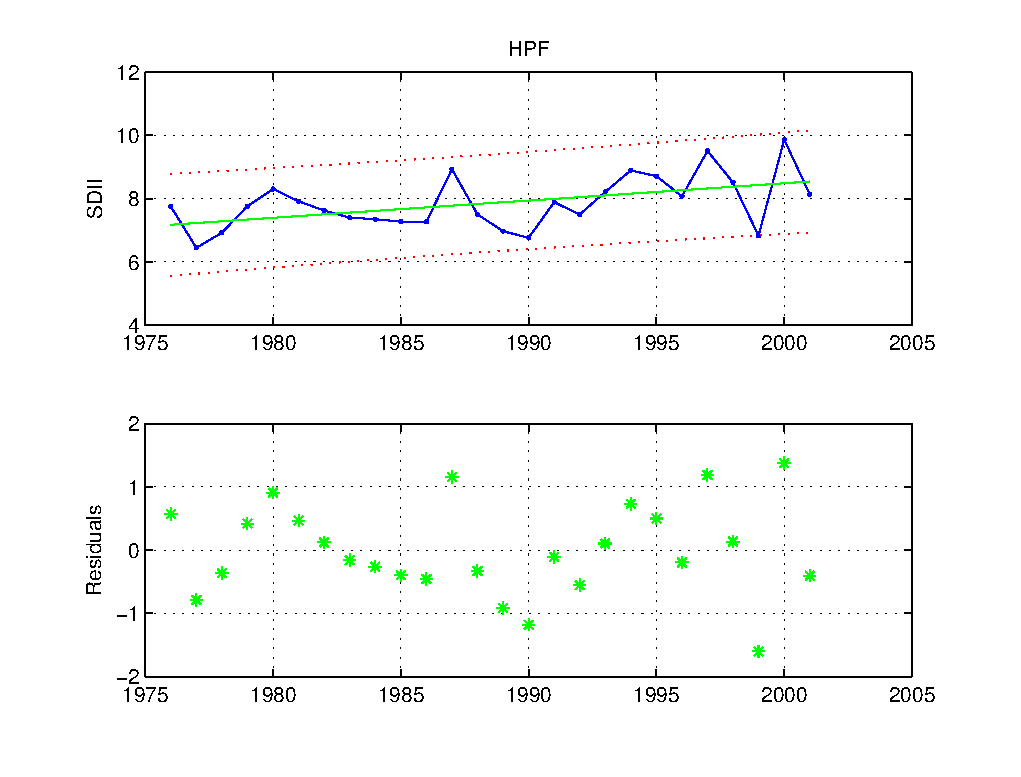
\includegraphics[width=0.33\textwidth]{./img/hpf_sdii}}

  \subfloat[HD]{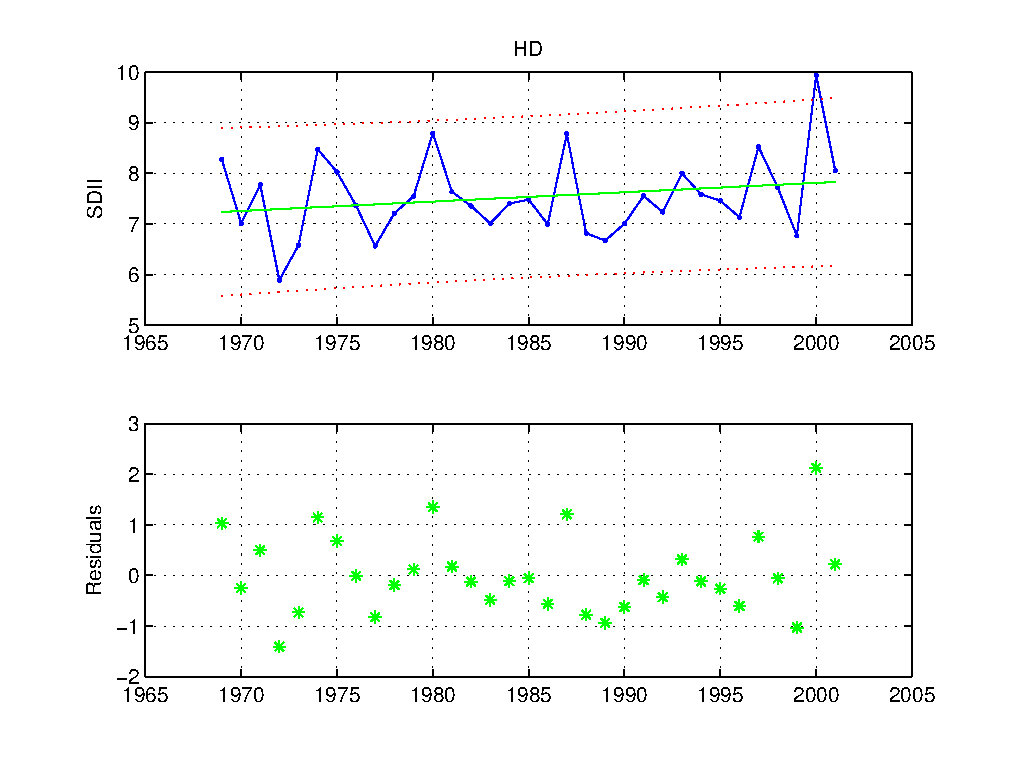
\includegraphics[width=0.33\textwidth]{./img/hd_sdii}}
  \subfloat[FF]{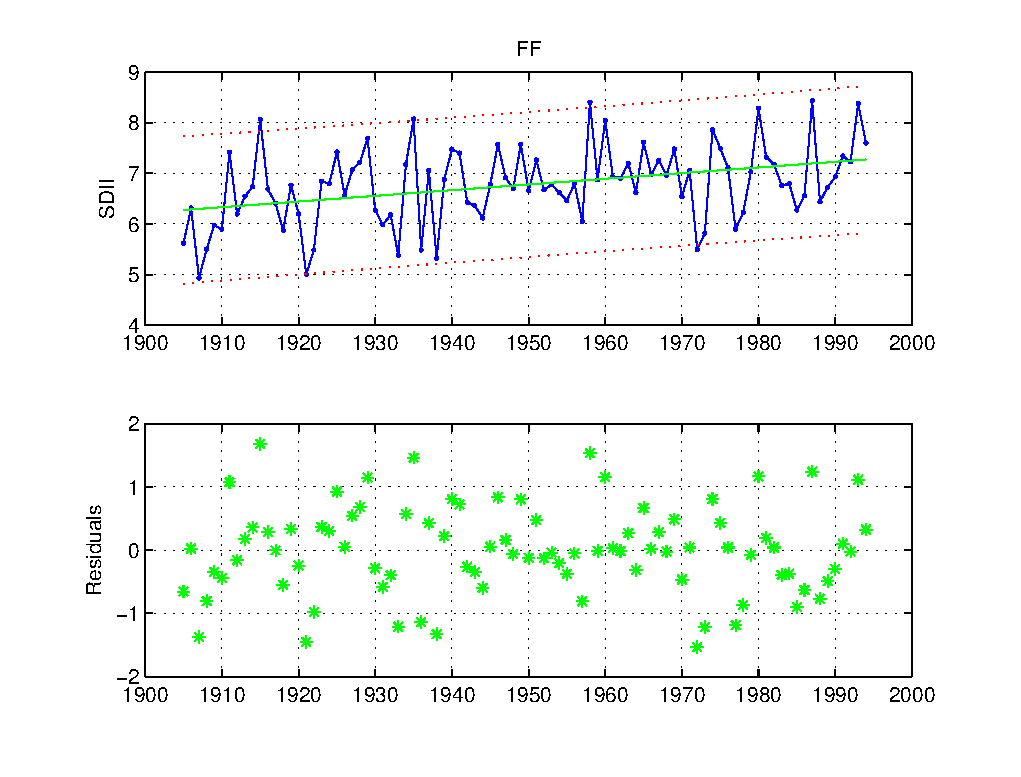
\includegraphics[width=0.33\textwidth]{./img/ff_sdii}}
  \caption{Trend of annual simple daily intensity index (SDII) at daily
data stations}
  \label{fig:FF_annual_SDII}
\end{figure}

\paragraph{Number of Days with Precipitation Amount $\geq$ 10 mm (R10mm)}
\label{sec:R10}
Annual trends of number of wet days with precipitation amount greater than 10 mm
(R10mm) from the studied stations are at variance. Only Falmer Farm Station
shows a statistically significant upwards trend for the 1971--1996 period (M-K,
$p<0.05$) (Figure \ref{fig:FF_annual_R10mm}). PL ($p < 0.05$) and FF ($p \ll
0.05$) show a statistically significant increasing trend in the annual ratio of
number of wet days with rainfall amount greater than 10 mm (Figure
\ref{fig:FF_annual_R10-b}).

\begin{figure}[htbp]
  \centering
  \subfloat[DR]{\includegraphics[width=0.33\textwidth]{./img/dr_r10mm}}
  \subfloat[SO]{\includegraphics[width=0.33\textwidth]{./img/so_r10mm}}
  \subfloat[PL]{\includegraphics[width=0.33\textwidth]{./img/pl_r10mm}}

  \subfloat[PB]{\includegraphics[width=0.33\textwidth]{./img/pb_r10mm}}
  \subfloat[SDR]{\includegraphics[width=0.33\textwidth]{./img/sdr_r10mm}}
  \subfloat[EW]{\includegraphics[width=0.33\textwidth]{./img/ew_r10mm}}

  \subfloat[FT]{\includegraphics[width=0.33\textwidth]{./img/ft_r10mm}}
  \subfloat[LI]{\includegraphics[width=0.33\textwidth]{./img/li_r10mm}}
  \subfloat[HPF]{\includegraphics[width=0.33\textwidth]{./img/hpf_r10mm}}

  \subfloat[HD]{\includegraphics[width=0.33\textwidth]{./img/hd_r10mm}}
  \subfloat[FF]{\includegraphics[width=0.33\textwidth]{./img/ff_r10mm}
\label{fig:FF_annual_R10-a}}
  \caption{Annual number of wet days with rainfall amount $\geq$ 10 mm at
daily data stations}
  \label{fig:FF_annual_R10mm}
\end{figure}

\begin{figure}[htbp]
  \centering
  \subfloat[DR]{\includegraphics[width=0.33\textwidth]{./img/dr_r10p}}
  \subfloat[SO]{\includegraphics[width=0.33\textwidth]{./img/so_r10p}}
  \subfloat[PL]{\includegraphics[width=0.33\textwidth]{./img/pl_r10p}}

  \subfloat[PB]{\includegraphics[width=0.33\textwidth]{./img/pb_r10p}}
  \subfloat[SDR]{\includegraphics[width=0.33\textwidth]{./img/sdr_r10p}}
  \subfloat[EW]{\includegraphics[width=0.33\textwidth]{./img/ew_r10p}}

  \subfloat[FT]{\includegraphics[width=0.33\textwidth]{./img/ft_r10p}}
  \subfloat[LI]{\includegraphics[width=0.33\textwidth]{./img/li_r10p}}
  \subfloat[HPF]{\includegraphics[width=0.33\textwidth]{./img/hpf_r10p}}

  \subfloat[HD]{\includegraphics[width=0.33\textwidth]{./img/hd_r10p}}
  \subfloat[FF]{\includegraphics[width=0.33\textwidth]{./img/ff_r10p}
\label{fig:FF_annual_R10-b}}
  \caption{Annual \% of wet days with rainfall amount $\geq$ 10 mm at
daily data stations}
  \label{fig:FF_annual_R10p}
\end{figure}

\paragraph{Number of Days with Precipitation Amount $\geq$ 20 mm (R20mm)}
\label{sec:R20}
No station shows a significant trend in the annual number of wet days with
rainfall greater than 20 mm. A trend in the annual ratio of number of wet days
with rainfall amount over 20 mm was not detectable as well (Figure
\ref{fig:FF_annual_R20mm}).

\begin{figure}[htbp]
  \centering
  \subfloat[DR]{\includegraphics[width=0.33\textwidth]{./img/dr_r20mm}}
  \subfloat[SO]{\includegraphics[width=0.33\textwidth]{./img/so_r20mm}}
  \subfloat[PL]{\includegraphics[width=0.33\textwidth]{./img/pl_r20mm}}

  \subfloat[PB]{\includegraphics[width=0.33\textwidth]{./img/pb_r20mm}}
  \subfloat[SDR]{\includegraphics[width=0.33\textwidth]{./img/sdr_r20mm}}
  \subfloat[EW]{\includegraphics[width=0.33\textwidth]{./img/ew_r20mm}}

  \subfloat[FT]{\includegraphics[width=0.33\textwidth]{./img/ft_r20mm}}
  \subfloat[LI]{\includegraphics[width=0.33\textwidth]{./img/li_r20mm}}
  \subfloat[HPF]{\includegraphics[width=0.33\textwidth]{./img/hpf_r20mm}}

  \subfloat[HD]{\includegraphics[width=0.33\textwidth]{./img/hd_r20mm}}
  \subfloat[FF]{\includegraphics[width=0.33\textwidth]{./img/ff_r20mm}
\label{fig:FF_annual_R20-a}}
  \caption{Annual number of wet days with rainfall amount $\geq$ 20 mm at
daily data stations}
  \label{fig:FF_annual_R20mm}
\end{figure}

\begin{figure}[htbp]
  \centering
  \subfloat[DR]{\includegraphics[width=0.33\textwidth]{./img/dr_r20p}}
  \subfloat[SO]{\includegraphics[width=0.33\textwidth]{./img/so_r20p}}
  \subfloat[PL]{\includegraphics[width=0.33\textwidth]{./img/pl_r20p}}

  \subfloat[PB]{\includegraphics[width=0.33\textwidth]{./img/pb_r20p}}
  \subfloat[SDR]{\includegraphics[width=0.33\textwidth]{./img/sdr_r20p}}
  \subfloat[EW]{\includegraphics[width=0.33\textwidth]{./img/ew_r20p}}

  \subfloat[FT]{\includegraphics[width=0.33\textwidth]{./img/ft_r20p}}
  \subfloat[LI]{\includegraphics[width=0.33\textwidth]{./img/li_r20p}}
  \subfloat[HPF]{\includegraphics[width=0.33\textwidth]{./img/hpf_r20p}}

  \subfloat[HD]{\includegraphics[width=0.33\textwidth]{./img/hd_r20p}}
  \subfloat[FF]{\includegraphics[width=0.33\textwidth]{./img/ff_r20p}
\label{fig:FF_annual_R20-b}}
  \caption{Annual \% of wet days with rainfall amount $\geq$ 20 mm at
daily data stations}
  \label{fig:FF_annual_R20p}
\end{figure}

%%%%%%%%%%%%%%%%%%%%%%%%%%%%%%%%%%%%%%%%%%%%%%%%%%%%%%%%%%
\section{Event Precipitation}
\label{sec:EventRainfallData}

The result of the trend investigation with event rainfall data showed no
significant trend in amount, duration and intensity. The trends are either not
detectable or inconclusive. Thus, monthly patterns of amount, duration and
intensity have been investigated. The observed daily rainfall amount, duration
and intensity---1-min peak intensity---are shown in Figure
\ref{fig:obs_daily_amount}, Figure \ref{fig:obs_daily_duration} and Figure
\ref{fig:obs_daily_peak_int}, respectively.

\begin{figure}[htbp]
  \centering
    \includegraphics[width=1.0\textwidth]{./img/obs_daily_amount}
  \caption{Observed daily rainfall amount}
  \label{fig:obs_daily_amount}
\end{figure}

\begin{figure}[htbp]
  \centering
    \includegraphics[width=1.0\textwidth]{./img/obs_daily_duration}
  \caption{Observed daily rainfall duration}
  \label{fig:obs_daily_duration}
\end{figure}

\begin{figure}[htbp]
  \centering
    \includegraphics[width=1.0\textwidth]{./img/obs_daily_peak_int}
  \caption[Observed daily 1-min peak rainfall intensity]{Observed daily
1-min peak rainfall intensity.}
  \label{fig:obs_daily_peak_int}
\end{figure}

The highest daily rainfall amount is 133.8 mm which fell on 11 October 2000 at
Plumpton. This rainfall is also the longest rainfall event which lasted for 443
minutes as a effective duration, which is over 7 hours (Figure
\ref{fig:obs_daily_duration}). The average intensity of the event was 18.1
mm/hr.

\paragraph{Rainfall Amount}
\label{sec:RainfallAmount}

The observed mean monthly rainfall amount is shown in Figure
\ref{fig:obs_mean_monthly_amount}. All the stations showed the October peak in
rainfall amount. Plumpton station showed a large difference of the rainfall
amount between October and June (Figure \ref{fig:obs_mean_monthly_amount}).

\begin{figure}[htbp]
  \centering
  \includegraphics[width=0.60\textwidth]{./img/obs_mean_monthly_amount}
  \caption[Observed mean monthly rainfall amount]{Observed mean monthly
rainfall amount}
  \label{fig:obs_mean_monthly_amount}
\end{figure}

\paragraph{Rainfall Duration}
\label{sec:RainfallDuration}

The mean monthly rainfall duration is shown in Figure
\ref{fig:obs_mean_monthly_duration}. The mean monthly rainfall duration shows
the similar characteristic October peak as the mean monthly rainfall amount.

\begin{figure}[htbp]
  \centering
  \includegraphics[width=0.60\textwidth]{./img/obs_mean_monthly_duration}
  \caption{Mean monthly rainfall duration}
  \label{fig:obs_mean_monthly_duration}
\end{figure}

\paragraph{Rainfall Intensity}
\label{sec:ResultsRainfallIntensity}

The maximum daily 1-min rainfall intensity series for Ditchling Road, Southover
and Plumpton are shown in Figure \ref{fig:obs_daily_peak_int}. The highest 1-min
peak intensity reaching at 300 mm/hr was observed on 5 November 1991 at
Ditchling Road (Figure \ref{fig:obs_daily_peak_int}).

The mean monthly maximum 1-min rainfall intensity is shown in Figure
\ref{fig:obs_mean_monthly_1min_intensity}. The highest values were observed in
November, September and August at Ditchling Road, at Southover and Plumpton,
respectively.

\begin{figure}
  \centering
  \includegraphics[width=0.60\textwidth]{%
./img/obs_mean_monthly_1min_intensity}
  \caption{Mean monthly maxima of 1-min peak rainfall intensity}
  \label{fig:obs_mean_monthly_1min_intensity}
\end{figure}

The mean monthly maximum 30-min rainfall intensity is shown in Figure
\ref{fig:obs_mean_monthly_30min_intensity}. The highest values were observed in
August, September and August at Ditchling Road, at Southover and Plumpton,
respectively.

\begin{figure}[htbp]
  \centering
  \includegraphics[width=0.60\textwidth]{%
./img/obs_mean_monthly_30min_intensity}
  \caption{Mean monthly maxima of 30-min peak rainfall intensity}
  \label{fig:obs_mean_monthly_30min_intensity}
\end{figure}

%%%%%%%%%%%%%%%%%%%%%%%%%%%%%%%%%%%%%%%%%%%%%%%%%%%%%%
\section{Discussion}
\label{sec:ObservedRainfallIntensityTrendsDiscussion}

%you imply that you are using present-day climate data to predict future
%erosion. No-one can do that! What you are doing, of course, is to create
%scenarios of future rainfall which are *based on* present-day rainfall (and
%then these are used to make predictions re. future erosion). *I* know that
%you know this, but the text isn't clear. Be as clear as possible: it is
%easy to create confusion in the mind of the reader if you are not
%completely clear.

Monthly 0.5\textdegree\ grid rainfall data provide a long-term rainfall trend
over a 100 year period. However, this trend is based on monthly mean rainfall
amount. Thus, no information on rainfall intensity is given.

Daily station rainfall data have been analysed to find out the trend in various
rainfall characteristics including daily rainfall intensity. These trends are
station specific, so that each station may have different trends in rainfall
from one to another. The daily intensity trend does provide a trend in rainfall
intensity. However, in general, sub-daily data are required to estimate soil
erosion using the present process-based models such as ones like WEPP, EUROSEM
and RillGrow which are used in this research.

It has been shown that the months of July and March have decreasing trends in
rainfall amount, that the annual number of wet days is declining, and that yet
the trend in daily rainfall intensity is increasing. It has also shown that
there is an increasing trend in the number of wet days with rainfall greater
than 10 mm at Falmer Farm and Plumpton stations. No station has shown a
significant trend in the annual number of wet days with rainfall greater than 20
mm. This is probably because there are only few records of such event. The
station with the longest data duration (FF) show about less than 5\%, on
average, are rainfall event with $\geq$20 mm, annually.

%******put the below in the result or data/method chapter

%Tipping-bucket rainfall data retain detailed information of rainfall which is
%close to data collected by a traditional pluviograph. With these data,
%sub-daily rainfall intensity data can be obtained. The tipping-bucket event
%data have been converted to 1-min data.

%The data were digitised to 1-min data. By doing this, rainfall intensity
%was converted to a minute increment. This means that rainfall intensity
%(mm/hr) for an increment is calculated as: rainfall amount (mm/min)
%$\times$ 60 $=$ rainfall intensity (mm/hr).

%This means that whatever the changes of intensity occurred during the 1-min
%interval is ignored, so the detectable intensity is limited to a minute. The
%reason for this conversion is two fold. One is for the ease of data handling.
%It is much more convenient to calculate rainfall amount, duration and intensity
%of rainfall data with a fixed time interval. Another is to remove the
%irregularity of the data. Because different formats were used for recording
%rainfall, some parts of the data were recorded as a number of tips per minute
%rather than the time of every single tip. Thus, all the data have been
%aggregated into 1-min scale, which is the shortest time step the data can be
%aggregated by. By converting the data to 1-min data, minimum rainfall intensity
%is defined to 12 mm/hr (i.e.\ 0.2 mm/1 min).

%Also, although this is not a very good conceptual model for multi-day storms
%(i.e.\ storms which last more than 24 hour), it is assumed that there is only
%one storm on a wet day. This is done to use the data for the WEPP simulation.

%******up to here

Tipping-bucket event data evidently gave greater detailed information about
rainfall intensity than the other two data types used here. Tipping-bucket event
data provide sufficient information about rainfall features for erosion
modelling such as duration and peak intensity of the rainfall event. The
rainfall parameters for soil erosion model simulation conducted in this research
are based on the tipping-bucket data shown in Table
\ref{tab:DetailsOfDataStations}. However, these kind of data may not be suitable
for trend studies.  This is partly due to the fact that they are not easily
accessible and not normally stored long-term.
% Rationale that is
%related to Downscaling. You need to explain why you did not go that way.
%Because there already is uncertainty with downscaling method as well as
%erosion model. Relate this with effect of data scale chapter.

The range of different scaled data gave some clues for future rainfall intensity
of the study site. The long-term records---monthly and daily---agree broadly
with the latest IPCC report, which suggests more extreme rainfall for the
future. However, it is not yet clear how extreme it is going to be.

To determine the rainfall \emph{intensity} trend for future erosion estimation,
one should have long term records of sub-daily rainfall records. The most common
and easily obtainable long term data are daily data. This may give a hint of
future rainfall intensity. However, with daily data alone, it is very difficult
to estimate rainfall intensity that is useful enough for soil erosion
prediction. The availability of sub-daily rainfall data with a long continuous
data period is very limited, so that it is very hard to find such data.
With intensive monitoring network growing worldwide, high resolution data (i.e.\
event data) are becoming more and more available to researchers.

There have been few short term high resolution rainfall data available for this
research. With this high resolution data, one may be able to obtain sufficient
rainfall intensity information for soil erosion modelling. This, however, is not
sufficient for trend estimation. This causes problems in estimating future soil
erosion. Simply put, there are not many sub-daily long term data records
available for studies like the present research which aims to find trend in
rainfall intensity.

Knowing the rainfall intensity trend is important for soil erosion estimation
for the future. However, detecting the rainfall intensity trend is very
problematic considering the variability of available rainfall data scales.
Different temporal scales and spatial scales can alter the trajectory of the
rainfall intensity trend greatly. Also, rainfall data coarser than a daily scale
can not give any useful rainfall intensity information for soil erosion
estimation as rainfall intensity patterns within a day can not be determined.

Daily rainfall duration can be seen in two ways. One is from the start of the
storm to the end of the storm. The other is a net duration, which is a sum of
the unit time steps during which the rainfall occurred. The latter concept has
been employed for rainfall intensity studies and WEPP (although the reason for
this choice is undocumented), despite the former definition being more
realistic.

The patterns of mean monthly peak rainfall intensity (e.g.\ 1-min peak) seem to
follow rainfall amount and rainfall duration at the studied stations. This means
the more the rain, the longer the duration, so that the higher the intense
rainfall intensity, in general. For example, when you get a short burst of high
intensity rainfall, the total rainfall amount may be relatively small. However,
it still exhibits a high rainfall intensity. High rainfall intensity is closely
related with high erodibility. Thus, it is important to look at the details of
rainfall intensity details including peak rainfall intensity for soil erosion
researches.

When an extreme rainfall event occurs, it may be a rainfall event either with
great quantity, with great intensity or with great quantity and intensity
together. This categorization is essentially dependent on one item of
information, namely time. It is also important to note that as the intensity is
time-dependent (the rate of rainfall), changing the time interval for intensity
calculation will results in different intensity patterns. This was the case for
Ditchling Road---the November peak in 1-min data was replaced by August peak in
30-min (Figure \ref{fig:obs_mean_monthly_1min_intensity} and Figure
\ref{fig:obs_mean_monthly_30min_intensity}). Thus, it may be useful to look for
trend of monthly rainfall intensity shift. The change of monthly rainfall
intensity may affect soil erosion because of the timing of tillage management.

Without the information on how long the event lasted, rainfall intensity can not
be calculated. Moreover, even if we do know the start and end time of the event,
there is no way we can determine intensity changes during the storm without the
data with appropriately fine scales. By knowing the start and end time, only the
average intensity over the storm duration will be obtainable. Most erosion
models nowadays---so-called process-based models---would not give useful
estimates of erosion with average intensity only. They require sub-daily
rainfall data.


%******added

Evidently, we need to know future WSIV, WSIP and WSG in order to improve erosion
prediction. As far as this research is aware, currently RCMs and GCMs rainfall
data have not been tested on these characteristics. However, it would not be
surprising to find these values predicted by RCM and GCM have high uncertainty
levels. Rainfall data should be studied more in detail by looking at these three
values and how they are related to erosion processes, so that these values can
be better incorporated into erosion models.

It already is difficult to find trend of intensity and 30-min peak intensity
using observed data. It will be even more difficult to predict future WSIV, WSIP
and WSG using climate model predicted data. Therefore, future scenarios have
been
built and simulated future erosion with the continuous model (i.e.\ WEPP).

%explain why is this approach is worthwhile.
%******

%Questions
%\begin{itemize}
% \item How climate change studies deal with rainfall intensity?
%$\rightarrow$ Mostly as daily intensity!
% \item Is the information appropriate for soil erosion (estimation)
%studies? If not, why?
% \item Then, what do we need to know about rainfall intensity in order to
%estimate future soil erosion?
%\end{itemize}

%To see how much they are different in terms of total rainfall amount
%
%To daily rainfall intensity and extreme events trends (RR1, R10mm and
%R20mm)
%
%Can we identify any trend in daily rainfall intensity? Or extreme events?
%
%Did this investigation give enough information on future rainfall
%intensity, so that we can work out soil erosion in the future? If not, what
%was the problem? Discuss.
%
%Compare observed rainfall trends in UK, USA and my findings
%
%more rain (quantity) in October, more intense rain (intensity) in August or
%September (according to event data).

\section{Conclusion}
\label{sec:ObservedRainfallIntensityTrendsConclusion}
We know rainfall amounts are going to be change in the future, but what about
intensity? \citet{trenberth2003-1205} calls more researches for this issue.

Despite the various efforts to find meaningful rainfall intensity trend for
building future scenarios of rainfall intensity changes, no significant trend
can be determined because of the great variability in the high resolution
rainfall data. It is necessary to draw out the significant trend from data with
sufficient scale that can be used in erosion modellings.

To achieve the aim of this research, an alternative method has to be sought to
obtain future rainfall data with a appropriate data scale and `changed' rainfall
intensity. The process of finding alternative method is discussed in the next
chapter (Section \ref{sec:ProposedSimulationMethods}).

This chapter has tried to answer the following research questions:
\begin{itemize}
  \item What are the main properties of present-day rainfall in the study site?
  \item Will the future rainfall intensity be different from the present?
If so, is it going to increase, decrease or stay the same?
\end{itemize}

In this chapter, it has been shown that:
\begin{enumerate}
  \item the month of July and March have decreasing trends in rainfall amount;
  \item the annual number of wet days is declining, and;
  \item yet the trend in daily rainfall intensity is increasing.
\end{enumerate}

It has also shown that there is an increasing trend in the number of wet days
with rainfall greater than 10 mm at Falmer Farm and Plumpton stations although
no station has shown a significant trend in the annual number of wet days with
rainfall greater than 20 mm.

During investigations of the rainfall trend, the following were recognized:
\begin{itemize}
  \item To determine the trend in rainfall intensity, the detailed rainfall
record is needed.
  \item Rainfall intensity trend is not the same as rainfall amount trend
  \item Duration of the data record limits validity of the trend.
  \item Availability of long-term high-resolution rainfall record is
paramount for the investigation into the trend in rainfall intensity.
\end{itemize}

%\nolinenumbers

%High intensity event (with 30-min data) in August (Ditchling Road and
%Plumpton) September (Southover).
%With 1-min data, high intensity in November (Ditchling Road), August
%(plumpton) and September (Southover)
%
%High amount in October (for all three stations)
%longest duration in October (Dichling and Plumpton) Southover showed long
%duration in October too but longest in December.
%
%These results are dependent on the amount and duration of data.
%
%The data used in the research showed that a greater amount of rainfall
%occurred mostly in the October months and high intensity events in August
%and September. This is because high amount events are events that lasted a
%long time with generally moderate intensity.


\part{Rainfall Intensity and Erosion: Model Descriptions and Responses}
\label{sec:RAINFALLINTENSITYCHANGESANDSOILEROSION}
%\linenumbers*

\chapter{IMPLICATION OF IMPROVED CLIGEN ON RAINFALL AND SOIL EROSION
SIMULATIONS}
\label{sec:IMPLICATIONSOFIMPROVEDCLIGEN}

\section{Introduction}
\label{sec:ImprovedCligenIntroduction}
CLIGEN, the weather generator for WEPP, went through extensive modifications
while the current research was carried out \citep{yu2000-301}. The modification
was done to improve CLIGEN in three respects. The first was the redefinition of
an input parameter, `{MX.5P}', which controls rainfall intensity generation in
CLIGEN. The second was the correction of the unit conversion error in
programming codes of CLIGEN. The third is a subsequent adjustment to remedy the
resulting unintended increases of simulated rainfall durations.

These changes prompted an investigation of their implications on rainfall
generations of CLIGEN and, in turn, soil erosion estimations of WEPP with CLIGEN
providing the input weather data. Before using the improved CLIGEN (i.e.\ CLIGEN
v5.2) for this research, it is important to understand how CLIGEN v5.2
performs and simulates weather data in comparison to the previous version.
A first reason for this is to gain insight into CLIGEN's operation. A second
reason is to see how these changes to CLIGEN affect the conclusions made by
previous publications on soil erosion under future climate change. A third
reason is that these changes may have invalidated previous sensitivity analyses
which involved CLIGEN v4.2
\citep{baffaut1996-447,zhang1996-855,baffaut1998-756,favis-mortlock1998-141,
favis-mortlock1999-329}.

Therefore, this chapter investigates effects of the changes of CLIGEN (from
version 4.2 to version 5.2) on rainfall data simulations and soil erosion
estimations by WEPP. During the investigation process, WEPP is also calibrated
and used for the subsequent simulations of this thesis.

\section{Data Preparation and Method for Model Simulation}
\label{sec:ImprovedCligenMethods}
Firstly, two CLIGEN input files---original and updated (see Appendix
\ref{sec:CLIGENInputData})---were prepared using the more recent rainfall data
(Table \ref{tab:DetailsOfDataStations}) obtained from the Ditchling Road site
(Figure \ref{fig:EventRainfallDataSite}). The original CLIGEN input file for
Ditchling Road was used in a study by \citet{favis-mortlock1998-141}. This file
was originally built with help from Arlin Nicks for David Favis-Mortlock in
1992\footnote{From personal communication with David Favis-Mortlock on 3 July
2001: \begin{quotation} ``My problem was that, in 1992, I did not have any
measured intensity data for the area. So, as I recall, I used maps in `NERC
(1975) \textit{Flood Studies Report}, Natural Environment Research Council,
HMSO, London' to pick out the maximum $x$-hour precipitation for each month for
the South Downs, where $x$ is something like 6 hours. The 1975 NERC report was
based on approximately 30 years of data. I then used a chart constructed from
empirical relationships in the 1975 NERC publication---Actually, from data given
to me by someone in the old Southern Water company, which data was drawn from
the 1975 NERC publication---to convert these values into 0.5-hour maxima. I then
sent these 0.5-hour max.\ values to Arlin. From these he calculated time-to-peak
values.'' \end{quotation}}. The newly prepared CLIGEN input file used event data
that have been measured since 1991 (Table \ref{tab:DetailsOfDataStations}).
`MEAN~P' (Table \ref{tab:UpdatedMEANPForDitchlingRoad}) and `{MX.5P}' (Table
\ref{tab:UpdatedMX5PForDitchlingRoad}) values of CLIGEN inputs were recalculated
using the up-to-date event data (Table \ref{tab:DetailsOfDataStations}). Note
that the units for these parameters are in inches, not in millimetres. Only
these two parameters were updated. The definition of the `{MX.5P}' was revised
by \citet{yu2000-301} following his discovery of the CLIGEN errors, so it was
recalculated accordingly in this research.

\begin{table}[htbp]
  \figureversion{tabular}
  \centering
  \caption[Original and Updated MEAN~P for Ditchling Road]{Original and
Updated MEAN~P (inches) for Ditchling Road}
  \label{tab:UpdatedMEANPForDitchlingRoad}
    \footnotesize
    \begin{tabular}{lrrrrrrrrrrrr}
    \toprule
     & Jan & Feb & Mar & Apr & May & Jun & Jul & Aug & Sep & Oct &
Nov & Dec\\
    \cmidrule{2-13}
    Original & 0.19 & 0.16 & 0.17 & 0.16 & 0.16 & 0.20 & 0.19 & 0.22
& 0.23 & 0.27 & 0.21 & 0.20\\
    Updated & 0.11 & 0.11 & 0.18 & 0.21 & 0.17 & 0.15 & 0.16 & 0.13
& 0.24 & 0.29 & 0.19 & 0.29\\
    \bottomrule
    \end{tabular}
\end{table}

\begin{table}[htbp]
  \figureversion{tabular}
  \centering
  \caption[Original and Updated {MX.5P} for Ditchling Road]{Original and
Updated {MX.5P} (in/hr) for Ditchling Road}
  \label{tab:UpdatedMX5PForDitchlingRoad}
    \footnotesize
    \begin{tabular}{lrrrrrrrrrrrr}
    \toprule
     & Jan & Feb & Mar & Apr & May & Jun & Jul & Aug & Sep & Oct &
Nov & Dec\\
    \cmidrule{2-13}
    Original & 0.63 & 0.59 & 0.55 & 0.55 & 0.55 & 0.55 & 0.55 & 0.67
& 0.79 & 0.93 & 0.87 & 0.75\\
    Updated & 0.27 & 0.18 & 0.23 & 0.23 & 0.27 & 0.33 & 0.42 & 0.58
& 0.43 & 0.45 & 0.34 & 0.30\\
    \bottomrule
    \end{tabular}
\end{table}

Next, continuous daily climate data for 30 years were generated with CLIGEN
version 4.1\footnote{There is virtually no difference between version 4.1 and
4.2 although version 4.2 was the one \citet{yu2000-301} found error in.} (old)
and version 5.2 (new) using these two input files. As a result, four datasets of
simulated climate data were generated (Table
\ref{tab:CLIGENSimulationSettingsWithDifferentInputsAndVersions}). These climate
data were compared in terms of rainfall amount, duration and peak intensity.

\begin{table}[htbp]
  \centering
  \small
  \caption{Weather simulation settings with different CLIGEN versions and inputs
for Ditchling Road}
  \label{tab:CLIGENSimulationSettingsWithDifferentInputsAndVersions}
  \begin{tabular}{ccc}
  \toprule
        & Original Input & Updated Input \\
  \midrule
  CLIGEN v4.1 & v4.1+original & v4.1+updated \\
  \midrule
  CLIGEN v5.2 & v5.2+original & v5.2+updated \\
  \bottomrule
  \end{tabular}
\end{table}

Two combinations of data and CLIGEN (i.e.\ v4.1+original and v5.2+updated) are
of the main concerns in this chapter because the other combinations (i.e.\
v5.2+original and v4.1+updated) have ``invalid'' combinations of MEAN~P and
{MX.5P}. Thus, the latter combinations will not give realistic results.
They are only considered here to highlight the changes of CLIGEN as a
sensitivity test.

Using WEPP, soil erosion rates for the same thirty-year period were, in turn,
estimated for Woodingdean site (Figure \ref{fig:WoodingdeanSite}) with each
CLIGEN-generated climate dataset. All other input data for the WEPP simulation
were acquired from the previous study by \citet{favis-mortlock1998-141}. Runoff
and soil loss rates were compared.
A Kolmogorov-Smirnov (K-S) test was used to test the null hypothesis that the
two populations are identical. Results of K-S test are presented in the next
section.

\section{Implication on Rainfall Data Simulation}
\label{sec:RainfallSimulation}

\subsection{Rainfall Amount}
Generated annual rainfall amounts for 30 years were within the range of the
reported annual rainfall amounts (750 and 1000 mm) in the area (Figure
\ref{fig:cligen_annual_amount}). The annual rainfall amounts generated by two
input files were not significantly different (K-S test, $p<0.05$). Although two
versions of CLIGEN resulted in a slight difference in annual rainfall amounts in
year 17 (Figure \ref{fig:cligen_annual_amount}), the differences between two
versions of CLIGEN were not statistically significant (K-S test, $p<0.05$).

\begin{figure}[htbp]
  \centering
   \includegraphics[width=0.8\textwidth]{./img/cligen_annual_amount_series}
  \caption{Simulated annual rainfall amount using two versions of CLIGEN with
original and updated input files.}
  \label{fig:cligen_annual_amount}
\end{figure}

\subsection{Rainfall Duration}
Contrastingly, simulated annual rainfall durations using two versions of CLIGEN
exhibited noticeable differences. CLIGEN v4.1 generated identical annual
rainfall durations even though two different input files (original
and updated) were used (Figure \ref{fig:cligen_annual_duration}). CLIGEN v5.2
generated markedly different rainfall durations when the same set of CLIGEN
input files were used (Figure \ref{fig:cligen_annual_duration}) (K-S test,
$p<0.05$).

\begin{figure}[htbp]
  \centering
\includegraphics[width=0.8\textwidth]{./img/cligen_annual_duration_series}
  \caption{Simulated annual rainfall duration using two versions of CLIGEN
with original and updated input files. Note that ``v4.1+original'' and
``v4.1+updated'' are in a complete overlap at each data point.}
  \label{fig:cligen_annual_duration}
\end{figure}

CLIGEN v5.2 with updated input file generated greatly increased rainfall
durations, almost 2.5 times longer on average than with original input file. The
rainfall duration (v5.2 + updated) was over 1.5 times longer on average in
comparison to the rainfall duration generated by CLIGEN v4.1 with both
original and updated input files. CLIGEN v5.2 with original input file
generated the shortest annual rainfall durations among the four series.
This means that, unlike old version, CLIGEN v5.2 is sensitive to the change of
two CLIGEN input parameters (i.e.\ MEAN~P and {MX.5P}), particularly to the
change of {MX.5P}. These large differences in rainfall durations mean that
rainfall intensities also differ greatly between the simulated rainfall
datasets.

\subsection{Monthly Maxima of Daily Peak Rainfall Intensity}
Next, monthly maxima of daily peak rainfall intensity series generated by CLIGEN
were compared in order to examine effects of extreme intensity events. The
results are shown in Figure \ref{fig:cligen_monthly_max_int}.

The Kolmogorov-Smirnov test indicates that CLIGEN v4.1 was not sensitive to the
changes of input files (See Figure \ref{fig:cligen_monthly_max_int}(a) and
\ref{fig:cligen_monthly_max_int}(c), $p<0.05$). In contrast, using original and
updated input files with CLIGEN v5.2 resulted in two significantly (K-S test,
$p<0.05$) different distributions of monthly maxima of daily peak rainfall
intensity (See Figure \ref{fig:cligen_monthly_max_int}(b) and
\ref{fig:cligen_monthly_max_int}(d)).
CLIGEN v5.2 generated fewer high intensity events than CLIGEN v4.1 (Figure
\ref{fig:cligen_monthly_max_int}(a)(c) and
\ref{fig:cligen_monthly_max_int}(b)(d)). There were, for example, only nine
monthly maxima of daily peak intensity over 100 mm/hr during 30 years of the
simulation period when CLIGEN v5.2 and updated input file were used (Figure
\ref{fig:cligen_monthly_max_int}(d)). Note that the magnitude of the monthly
maxima of the daily peak intensity seems to be in a similar range for all four
cases although the frequency of the high peaks are different depending on the
version of CLIGEN and input files (Figure \ref{fig:cligen_monthly_max_int}).

\begin{figure}[htbp]
  \centering

\includegraphics[width=0.8\textwidth]{./img/cligen_monthly_max_int_org}

\includegraphics[width=0.8\textwidth]{./img/cligen_monthly_max_int_mod}
  \caption[Simulated monthly maxima of daily peak rainfall intensity using
two versions of CLIGEN with original and updated input files]{Simulated monthly
maxima of daily peak rainfall intensity using two versions of CLIGEN with
original and updated input files. (a) CLIGEN v4.1 with original input file; (b)
CLIGEN v5.2 with original input file; (c) CLIGEN v4.1 with updated input file;
(d) CLIGEN v5.2 with updated input file.}
  \label{fig:cligen_monthly_max_int}
\end{figure}

\begin{figure}[htbp]
  \centering
    \includegraphics[width=0.8\textwidth]{./img/cligen_monthly_max_int_by_month}
  \caption{CLIGEN-generated mean monthly maxima of daily peak intensity
using two versions of CLIGEN with original and updated input files}
  \label{fig:cligen_dr_monthly_max_int_by_month}
\end{figure}

Mean monthly maxima of daily peak intensity were compared in Figure
\ref{fig:cligen_dr_monthly_max_int_by_month}. CLIGEN v4.1 with two input files
generated generally high mean monthly values through out most of months in
comparison to CLIGEN v5.2. The effect of different input files was very small
on CLIGEN v4.1 for simulating mean monthly maxima of daily peak intensity.
CLIGEN v4.1 generated highest mean monthly maxima of daily peak intensity in
October and lowest values in June with both input files. In contrast, CLIGEN
v5.2 generated significantly different mean monthly maxima of daily peak
intensity with two input files (K-S test, $p<0.05$). Much greater mean monthly
maxima of daily peak intensity were generated with v5.2+original than with
v5.2+updated. With original input file, CLIGEN v5.2 showed a peak in November
and a low in May.

With exception of v5.2+updated, all three simulations show generally high mean
monthly maxima of daily peak intensity in October and November and low mean
monthly maxima of daily peak intensity in April, May and June. When CLIGEN v5.2
with updated input file were used for the simulation, the monthly pattern was
very different from that of the other three combinations. In other words,
CLIGEN v5.2 with updated input file (v5.2+updated) simulated more realistic
monthly rainfall intensity.
This combination (i.e.\ v5.2+updated) showed relatively high mean monthly
maxima of daily peak intensity during the summer months (June, July and August)
with a distinctively high peak in August (Figure
\ref{fig:cligen_dr_monthly_max_int_by_month}). Generally low mean monthly maxima
of daily peak intensity in the rest of months were simulated with lowest mean
monthly maxima of daily peak intensity in March and April (Figure
\ref{fig:cligen_dr_monthly_max_int_by_month}). With updated input file and
CLIGEN v5.2, more high intensity events were simulated in the summer than the
autumn or winter in comparison to the other simulation combinations. This result
is closely similar to observed rainfall intensity found previously (Figure
\ref{fig:obs_mean_monthly_30min_intensity}).
%reason for this result can be explained by looking at the input files, october
%and august, MEAN P and MX .5P

\section{Implication on Runoff and Soil Erosion Simulation}
\label{sec:RunoffAndSoilLossSimulation}
Before starting investigations on effects of improved CLIGEN (i.e.\ CLIGEN v5.2)
on WEPP simulations, initial tests of WEPP were carried out with weather
generated by CLIGEN v5.2 with updated input file. The tests revealed that
uncalibrated WEPP overestimates mean soil loss by about 630\% in comparison to
observed soil losses from the study area (Table
\ref{tab:SimulatedSoilLossWithCLIGENV52WithUpdatedInput}). This erosion rate is
considered unrealistically high for the study site so that calibrations is
considered essential.

\begin{table}[htbp]
  \figureversion{tabular}
  \centering
  \caption[Simulated annual average runoff on hillslopes using
CLIGEN-generated weather with updated input]{Simulated annual average runoff
(mm) on hillslopes (D-L) using CLIGEN-generated (v5.2) weather with updated
input}
  \label{tab:SimulatedRunoffWithCLIGENV52WithUpdatedInput}
  \small
    \begin{tabular}{lrrrrrrrrrr}
      \toprule
      & D & E & F & G & H & I & J & K & L & Mean\\
      \cmidrule{2-11}
      uncalib. & 106.7 & 105.3 & 106.5 & 106.0 & 106.1 & 107.1 & 107.8 & 108.0 &
108.8 & 106.9\\
      recalib. & 74.2 & 72.9 & 73.9 & 73.6 & 73.4 & 74.3 & 74.8 & 75.2 & 75.9 &
74.2\\
      \bottomrule
    \end{tabular}
\end{table}

\begin{table}[htbp]
  \figureversion{tabular}
  \centering
  \caption[Simulated annual average soil loss on hillslopes using
CLIGEN-generated weather with updated input]{Simulated annual average soil loss
(t/ha) on hillslopes (D-L) using CLIGEN-generated (v5.2) weather with updated
input}
  \label{tab:SimulatedSoilLossWithCLIGENV52WithUpdatedInput}
  \footnotesize
    \begin{tabular}{lrrrrrrrrrr}
      \toprule
      & D & E & F & G & H & I & J & K & L & Mean\\
      \cmidrule{2-11}
      uncalibrated & 49.4 & 42.9 & 76.1 & 96.5 & 117.5 & 111.1 & 105.3 & 84.1 &
79.7 & 84.7\\
      recalibrated & 3.4 & 3.2 & 11.1 & 18.2 & 23.7 & 21.3 & 17.3 & 9.8 & 7.9 &
12.8\\
      measured$^a$ (m$^3$/ha) & 3.4 & 7.8 & 13.7 & 17.5 & 21.4 & 9.6 & 11.6 &
11.2 & 8.1 & 11.6\\
      \bottomrule
      %\addlinespace[1mm]
      \multicolumn{8}{l}{\footnotesize $^a$ over the periods of 1985-1986
\citep[From][]{favis-mortlock1998-141}}
    \end{tabular}
\end{table}

Thus, WEPP was calibrated by adjusting hydrological and
erosional parameter values. The adjusted parameters were shown in Table
\ref{tab:HydrologicalAndErosionalParameters}. Simulated runoff and soil
loss rates using uncalibrated and calibrated WEPP are presented in Table
\ref{tab:SimulatedRunoffWithCLIGENV52WithUpdatedInput} and
\ref{tab:SimulatedSoilLossWithCLIGENV52WithUpdatedInput}. There were no measured
runoff data available for the site although annual soil loss data for a short
period were acquired from \citet{favis-mortlock1998-141}.

\paragraph{Why calibrate?} When a erosion model is used for soil loss
estimations, it is important to note that the relationship of model inputs and
outputs is non-linear \citep{favis-mortlock1995-365,jetten1999-521}. For
example, say, we ran a erosion model with \emph{Input A} and got \emph{Output B}
(Figure \ref{fig:calibration}).

\begin{figure}[htbp]
  \centering
    \includegraphics[width=0.5\textwidth]{./img/calibration}
  \caption{A graphical representation of non-linear responses of a erosion
model}
  \label{fig:calibration}
\end{figure}

Then, in order to find possible effects of changes in inputs, we may change
\emph{Input A} to \emph{Input A'}. When the model was run with \emph{Input A'},
the responding model output should be \emph{Output B'} if the model has a linear
relationship between inputs and outputs. However, because of the non-linear
relationship, the responding output may be rather unknown \emph{Output B''}
(Figure \ref{fig:calibration}). This means that, unless model inputs and outputs
are identified and the model is calibrated against known output values, it may
be difficult to measure the extent of changes in model predictions.

Therefore, it is unlikely that non-calibrated models will lead to reasonable
simulation results. \citet{wainwright2008-813} also pointed out that, because
of the impossibility of theoretically deriving or measuring appropriate
parameters such as flow sheer stress, existing process-based erosion models
like WEPP and EUROSEM require calibration. However, even after calibration,
there still is the possibility of ending up with `the right answer for the wrong
reason' \citep{favis-mortlock1994-use}. This is, for example, because two or
more model inputs cancel each other out (or enhance each other) by unknown
interactions.

WEPP-simulated annual runoff and soil loss rates using four CLIGEN-generated
weather series are shown in Figure \ref{fig:cligen_annual_runoff_serise} and
Figure \ref{fig:cligen_annual_sloss_series}, respectively.

\begin{figure}[htbp]
  \centering
  \subfloat[]{%
  \label{fig:cligen_annual_runoff_serise_a}
  \includegraphics[width=0.49\textwidth]{%
./img/cligen_annual_runoff_serise_old_original}}
  \subfloat[]{%
  \label{fig:cligen_annual_runoff_serise_b}
  \includegraphics[width=0.49\textwidth]{%
./img/cligen_annual_runoff_serise_old_updated}}
  \qquad
  \subfloat[]{%
  \label{fig:cligen_annual_runoff_serise_c}
  \includegraphics[width=0.49\textwidth]{%
./img/cligen_annual_runoff_serise_new_original}}
  \subfloat[]{%
  \label{fig:cligen_annual_runoff_serise_d}
  \includegraphics[width=0.49\textwidth]{%
./img/cligen_annual_runoff_serise_new_updated}}
  \caption[Simulated annual runoff for Ditchling Road]{Simulated annual
runoff for Ditchling Road simulated with (a) CLIGEN v4.1 with original input
file; (b) CLIGEN v4.1 with updated input file; (c) CLIGEN v5.2 with original
input file; (d) CLIGEN v5.2 with updated input file. Note the same Y-axis scale
in all plots.}
  \label{fig:cligen_annual_runoff_serise}
\end{figure}

\begin{figure}[htbp]
  \centering
  \subfloat[]{%
  \label{fig:cligen_annual_sloss_series_a}
  \includegraphics[width=0.49\textwidth]{%
./img/cligen_annual_sloss_serise_old_original}}
  \subfloat[]{%
  \label{fig:cligen_annual_sloss_series_b}
  \includegraphics[width=0.49\textwidth]{%
./img/cligen_annual_sloss_serise_old_updated}}
  \qquad
  \subfloat[]{%
  \label{fig:cligen_annual_sloss_series_c}
  \includegraphics[width=0.49\textwidth]{%
./img/cligen_annual_sloss_serise_new_original}}
  \subfloat[]{%
  \label{fig:cligen_annual_sloss_series_d}
  \includegraphics[width=0.49\textwidth]{%
./img/cligen_annual_sloss_serise_new_updated}}
  \caption[Simulated annual soil loss for Ditchling Road]{Simulated annual
soil loss for Ditchling Road simulated with (a) CLIGEN v4.1 with original input
file; (b) CLIGEN v4.1 with updated input file; (c) CLIGEN v5.2 with original
input file; (d) CLIGEN v5.2 with updated input file. Note the same Y-axis scale
in all plots.}
  \label{fig:cligen_annual_sloss_series}
\end{figure}

Annual runoff and soil loss rates were not significantly affected by the use of
weather datasets that have been generated by CLIGEN v4.1 with two input
files (original and updated). Annual runoff (Figure
\ref{fig:cligen_annual_runoff_serise_a} and Figure
\ref{fig:cligen_annual_runoff_serise_b}) and annual soil loss rates (Figure
\ref{fig:cligen_annual_sloss_series_a} and Figure
\ref{fig:cligen_annual_sloss_series_b}) were almost identical between the two
configurations (v4.1+original and v4.1+updated). However, this is reasonable
given that there is little difference in the rainfall amounts and peak rainfall
intensities for these combinations (Figure \ref{fig:cligen_monthly_max_int}).

Mean annual runoff and soil loss rates estimated using weather data generated by
v4.1+updated were slightly decreased by 1.4\% and increased by 1.5\%
respectively in comparison to the estimation done by the use of weather data
generated with v4.1+original
(Table \ref{tab:SimualtedAnnualRunoffAndSoilLossWithDifferentConfiguration}).

\begin{table}[htbp]
  \figureversion{tabular}
  \centering
  \caption[WEPP-simulated average annual runoff and soil loss]{WEPP-simulated
average annual runoff (mm) and soil loss (t/ha) with CLIGEN-generated
weather with four different configurations.}
  \label{tab:SimualtedAnnualRunoffAndSoilLossWithDifferentConfiguration}
    \begin{tabular}{lrrrr}
      \toprule
       & \multicolumn{2}{c}{CLIGEN v4.1} &
\multicolumn{2}{c}{CLIGEN v5.2}\\
      \cmidrule(r){2-3}\cmidrule(l){4-5}
       & original input & updated input & original input &
updated input \\
      \midrule
      Runoff & 122.1 & 120.4 ($-$1.4) & 126.5 ($+$3.6) & 74.2 ($-$39.2)\\
      Soil Loss & 33.6 & 34.1 ($+$1.5) & 34.4 ($+$2.4) & 12.8 ($-$61.9)\\
      \bottomrule
      %\addlinespace[1mm]
      \multicolumn{5}{p{10.5cm}}{\footnotesize Figures in (\ )
represent \% differences from CLIGEN v4.1+original input file. $+/-$ sign
indicates an increase/decrease.}
    \end{tabular}
\end{table}

When both CLIGENs (v4.1 and v5.2) were run with original input file to generate
weather data, subsequent WEPP estimations of average annual runoff and soil loss
were not much different between the two versions of CLIGEN. Average annual
runoff and soil loss were only increased by 3.6\% and 2.4\%, respectively.
(Table \ref{tab:SimualtedAnnualRunoffAndSoilLossWithDifferentConfiguration}).

WEPP estimated considerably decreased runoff and soil loss rates when rainfall
data generated by CLIGEN v5.2 with the updated input file were used (Figure
\ref{fig:cligen_annual_runoff_serise_d} and Figure
\ref{fig:cligen_annual_sloss_series_d}) in comparison to the other three
configurations (Figures \ref{fig:cligen_annual_runoff_serise_a}--c and Figures
\ref{fig:cligen_annual_sloss_series_a}--c). In comparison to mean runoff and
soil loss rates estimated using rainfall data generated by CLIGEN v4.1 with
original input file, the runoff and soil loss rates decreased by about 39\% and
about 62\% respectively when rainfall data generated by CLIGEN v5.2 with updated
input file were used for WEPP simulations (Table
\ref{tab:SimualtedAnnualRunoffAndSoilLossWithDifferentConfiguration}).
The importance of these results are discussed in the following section.

\paragraph{Relative vs Absolute Model Output} In this research, both relative
(\% change) and absolute (t/ha) values were used for model outputs. It may seem
more meaningful to use only relative representations (\% change) of model
outputs than to use absolute values (t/ha) together with \% changes because what
this research is interested in is how model estimates change as a result of
rainfall intensity changes. However, in order to make a right judgement and to
assess estimated values correctly, we need both expressions: relative and
absolute. For instance, if a model estimates soil loss of 1000 t/ha from
a 1 m$\times$1 m plot after 10 mm/hr rainfall, it would hardly be considered
realistic, and the model and its inputs may need to be checked to find a reason
for the error. On the other hand, when a model estimates soil loss that changes
from, say, 0.00001 t/ha to 0.00002 t/ha, the \% change would be 100\% despite
the fact that this value can be seen as very trivial in the real world. Thus,
presenting the model result either only in relative (\% change) or absolute
(t/ha) value is probably misleading. Therefore, both expressions are used in
this research when simulation results are presented.
%Also, calibrations carried
%out previously provide robust realistic absolute values.

\section{Discussion}
\label{sec:ImprovedCLIGENDiscussion}

\subsection{Impact on Rainfall Intensity Generation}

\citet{yu2000-301} suggests that CLIGEN became sensitive to the change of the
rainfall intensity parameter because of the improvement. This investigation
confirms this improvement. Rainfall duration generated by CLIGEN v5.2
showed a clear signs of the sensitivity to the change of rainfall intensities
which is shown in Figures \ref{fig:cligen_annual_duration} and
\ref{fig:cligen_dr_monthly_max_int_by_month}.

The updated CLIGEN input file has lower {MX.5P} values than original input file.
This difference led to longer rainfall durations generated by CLIGEN v5.2
as shown in Figure \ref{fig:cligen_annual_duration}. This was expected because
of the lower {MX.5P} values and the similar MEAN~P values in updated input file
in comparison to the same parameters in original input file (Figure
\ref{fig:mean_p_mx5p_cligen}). With the rainfall amount being almost
unchanged---only slightly changed, but statistically the same ($p<0.05$),
rainfall duration has to be increased to satisfy low intensity parameters
(Figure \ref{fig:mean_p_mx5p_cligen}). This, in turn, decreases rainfall
intensities generated by CLIGEN v5.2 (Figure
\ref{fig:cligen_dr_monthly_max_int_by_month}, v5.2 + updated).

\begin{figure}[htbp]
  \centering
    \subfloat[MEAN P]{\label{fig:mean_p_cligen}
\includegraphics[width=0.49\textwidth]{./img/mean_p_cligen}}
    \subfloat[MX .5P]{\label{fig:mx5p_cligen}
\includegraphics[width=0.49\textwidth]{./img/mx5p_cligen}}
  \caption[Mean daily precipitation depth and mean maximum daily 30-minute
rainfall intensity for each month]{Mean daily precipitation depth (inch) and
mean maximum daily 30-minute rainfall intensity (in/hr) for each month. Note
that the units are in inches, not in millimetres, as CLIGEN requires these
values in inches.}
  \label{fig:mean_p_mx5p_cligen}
\end{figure}

CLIGEN(v4.1 did not show clear changes in rainfall intensity even though
the rainfall intensity parameter ({MX.5P}) were updated to the lower values when
the input file was prepared. This insensitivity of CLIGEN v4.1 is the
result of the unit conversion error previously found by \citet{yu2000-301}.
Correcting the errors in the previous version of CLIGEN resulted in the
decreased rainfall intensity (Figure
\ref{fig:cligen_dr_monthly_max_int_by_month}).

One interesting finding is that when the original CLIGEN input file was used for
both climate simulations with CLIGEN v4.1 and v5.2, rainfall durations generated
by two CLIGENs were not significantly different so thus resulting intensities.
This finding may be explained by the differences in two versions of CLIGEN.
CLIGEN v5.2, as shown earlier, is much more sensitive to changes in rainfall
intensity than CLIGEN v4.1, so that, with the CLIGEN input file that has
low rainfall intensity (i.e.\ Updated CLIGEN input), CLIGEN v5.2 will
simulate rainfall data with much lower rainfall intensity, hence longer rainfall
durations. This has been shown previously. What is more interesting is that,
in contrast, with CLIGEN input file that has high rainfall intensity
(i.e.\ original CLIGEN input), CLIGEN v5.2 still simulate climate data
with corresponding rainfall intensity, that is high rainfall intensity, hence
short rainfall durations. This is more evident as CLIGEN v5.2 generated
shorter annual rainfall durations with original input file (Figure
\ref{fig:cligen_annual_duration}) than CLIGEN v4.1 with original (or
updated) input file. However, when mean monthly maxima of daily peak intensity
were compared as shown in Figure \ref{fig:cligen_dr_monthly_max_int_by_month},
CLIGEN v5.2 generated lower values for mean monthly maxima of daily peak
intensity than CLIGEN v4.1 with both input files.

Overall, this finding means that the improvement of CLIGEN has smaller impacts
on weather generations for locations where high intensity rainfall events are
dominant.

Moreover, CLIGEN v5.2 with the updated input file simulated a peak monthly
intensity in August (Figure \ref{fig:cligen_dr_monthly_max_int_by_month}) that
can also be seen in the input file (Figure \ref{fig:mx5p_cligen}). This means
that CLIGEN v5.2 generates monthly rainfall intensity that are similar
to {MX.5P} values which are calculated from observed weather data. CLIGEN v4.1,
on the other hand, generated the similar monthly rainfall intensity for both
CLIGEN input files. This implies that CLIGEN v4.1 does not recognize the
intensity differences introduced by the different {MX.5P} parameters in the
input files.

Therefore, it is strongly suggested to use CLIGEN v5.2 for all future
studies. It is also advisable to review previous CLIGEN input files when
possible.

\subsection{Impact on Subsequent WEPP Simulation}

Runoff and soil erosion rates estimated by WEPP showed similar responses to
those from the analysis of rainfall generations. This implies that WEPP is
sensitive to the changes of climate data which have been used for the
simulation.

The two identical climate datasets generated by CLIGEN v4.1 with two input
files (original and updated) did not affect WEPP-estimated annual runoff
(Figures \ref{fig:cligen_annual_runoff_serise_a} and
\ref{fig:cligen_annual_runoff_serise_b}) and soil erosion rates (Figures
\ref{fig:cligen_annual_sloss_series_a} and
\ref{fig:cligen_annual_sloss_series_b}).
There were slight differences between two settings in terms of average annual
runoff and soil loss rates (Table
\ref{tab:SimualtedAnnualRunoffAndSoilLossWithDifferentConfiguration}). The
differences were however questionable as average annual soil loss rate was
increased even though average annual runoff was decreased.

The use of two climate datasets generated by CLIGEN v5.2 with original and
updated input files resulted in significantly different runoff and soil loss
rates. WEPP simulated considerably lower annual runoff and soil loss rates when
climate data generated by CLIGEN v5.2 with updated input file were used
than when climate data generated by CLIGEN v5.2 with original input file
were used. This is because of the increased rainfall duration which have
been caused by the decreases in rainfall intensity (Figure
\ref{fig:cligen_annual_duration}). Considering that simulated rainfall amounts
were not much different in both input files of CLIGEN, it is evident that low
rainfall intensity is the reason for the low annual runoff and annual soil loss
rates estimated by WEPP.

Therefore, the implication of the improvement in CLIGEN is relatively small when
CLIGEN was used to simulate climate data for a place where rainfall events
with high intensity are dominant. On the other hand, when CLIGEN was used
to generate climate data for a place where rainfall events with low intensity
are dominant (e.g.\ South Downs, UK), differences of climate data simulated by
CLIGEN v4.1 and v5.2 would be so great that subsequent WEPP estimations will be
greatly affected and erroneous estimations are inevitable.

In the next section, some examples of previously published studies that may have
been affected by these CLIGEN improvements are subjectively selected and
discussed to highlight the implication of the CLIGEN improvement.

\subsection{Implication for Previously Published Studies Prior to CLIGEN v5.2}

Thus, published papers that used CLIGEN v4.1, prior to \citet{yu2000-301}, to
generate weather data are theoretically affected by the improvement. The
magnitude of effects can vary depending on characteristics of typical rainfall
storms in study area as shown in the present research.

\paragraph{\citet{baffaut1996-447}} used CLIGEN v4.1 to generate 200 years of
climate data for WEPP simulations in order to investigate impacts of CLIGEN
parameters on WEPP-predicted average annual soil loss. The study found that only
five parameters, that are mean precipitation per event, standard deviation of
the precipitation per event, skewness of the precipitation per event,
probability of a wet day following a wet day and probability of a wet day
following a dry day, influenced the estimated average annual soil loss. However,
they found that half hour largest intensity (i.e. {MX.5P}) and the statistical
distribution of the time to peak had less influence on the output. Insensitivity
to {MX.5P} parameter, which \citet{baffaut1996-447} found, could be the result
of the error found in CLIGEN v4.1 as \citet{yu2000-301} pointed out.

However, it is also possible that the insensitivity to {MX.5P} was from
the characteristic of rainfall storms in the study area. \citet{baffaut1996-447}
considered Indiana, Alabama, Kansas, Colorado, Washington and Virginia, USA. It
is suggested that storms with high rainfall intensity is common in the central
and eastern United States \citep{ashley2003-3003}. This means that the magnitude
of effects from CLIGEN improvements could be smaller because the studied
area are mostly in the central or eastern US except Washington. As shown in
Table \ref{tab:SimualtedAnnualRunoffAndSoilLossWithDifferentConfiguration},
areas with high rainfall intensity are less influenced by the improvement of
CLIGEN.

Therefore, the information and analysis from \citet{baffaut1996-447} do not
provide any conclusive evidence to determine the effect of improved CLIGEN.

\paragraph{\citet{zhang1996-855}} conducted a study to evaluate the overall
performance of
WEPP in predicting runoff and soil loss under cropped conditions. They also used
CLIGEN v4.1 to generate the weather parameters in the WEPP climate input files.
Although they used CLIGEN, not all weather parameters were generated by CLIGEN.
Values for amounts of rainfall, rainfall duration, time to peak intensity and
ratio of mean to peak intensity were directly calculated from measured rainfall
data for each storm at all the sites they considered. This means that their
study may not greatly affected by the change of CLIGEN. As this chapter
suggested, rainfall duration and intensity are the most affected parameters in
WEPP climate inputs.

\paragraph{\citet{baffaut1998-756}} also used CLIGEN v4.1 to generate synthetic
weather series to analyse frequency distributions of measured daily soil loss
values and to determine if the WEPP accurately reproduced statistical
distributions of the measured daily erosion series. The sites that they selected
for their study were in the eastern USA. They selected the study sites based on
length of records, the number of events recorded, and the uniformity of the
management practices. This means that the series of weather data generated by
CLIGEN v4.1 may not have been different statistically compared to measured
values because of the high rainfall intensity for their study sites
\citep{ashley2003-3003}.
The paper did not include the result of weather simulations. However, it
was indicated that CLIGEN-generated data were not statistically different from
monitored weather data. Thus, this paper also elaborates that the implication of
the change of CLIGEN is small when CLIGEN v4.1 was used to generated weather
data for areas with high rainfall intensity.

\paragraph{\citet{favis-mortlock1999-329}} conducted a case study from Brazil to
suggest an
approach to quantifying the change in risk of serious erosion for venerable
areas. \citet{favis-mortlock1999-329} used CLIGEN v4.1 to generate 100 years of
weather data based on current-climate and, then, used three GCMs to perturb 100
years of CLIGEN-generated daily weather data. The area which
\citet{favis-mortlock1999-329} studied has several monsoon characteristics in
addition to the distinct wet and dry seasons \citep{gan2004-47}. This means
that the area have a large variability in rainfall intensity, which implies
that impacts of the change of CLIGEN could be small on the overall result of the
paper. However, it could still be possible that rainfall duration and number of
extreme events could have been overestimated somewhat.

The previously published paper that were discussed here used CLIGEN v4.1 for
generating weather data. This implies that articles may have been affected by
the previous errors of CLIGEN to a certain extend. However, the information
included in these articles does not have enough details to determine the extend
and the effect of improvements of CLIGEN. Yet, the magnitude of impacts varies
depending on how CLIGEN was used and where CLIGEN was used for. In summary,
it is evident that previously published papers that uses CLIGEN v4.1 to
generate weather data for the area, like the central and eastern US or central
South America, where high intensity storm is common are not greatly affected,
at least, not as much as other places like the southern England where low
intensity rainfall is common.

\section{Conclusion}
\label{sec:ImprovedCLIGENConclusion}
The improvement of CLIGEN has important implications on generating synthetic
climate data and subsequent WEPP simulations in runoff and soil loss rates.
CLIGEN v4.1 is not sensitive to changes of rainfall intensity. The previous
version generates the similar climate series with original and updated CLIGEN
input files that have high and low intensity parameters, respectively. However,
CLIGEN v5.2 is now sensitive to changes of rainfall intensity which is
parameterized as {MX.5P}. The effect of the improvement of CLIGEN is more
(less) significant for the regions where low (high) intensity rainfall events
are dominant.
All previous articles that used the previous versions of CLIGEN (v4.1 or older)
may have been affected by the errors of CLIGEN v4.1 to a certain extend.
However, the magnitude of impacts varies depending on how CLIGEN was used and
where CLIGEN was used for. It could have been catastrophic to find out the
errors of CLIGEN at the later stage of this research because the site where this
research is based on is South Downs, UK where impacts of the improvement of
CLIGEN are great as discussed previously.

%\nolinenumbers


%\linenumbers*
\chapter{EFFECT OF TEMPORAL SCALES OF STORM DATA ON EROSION}
\label{sec:EFFECTSOFTEMPORALSCALESOFSTROMDATA}

\section{Introduction}
\label{sec:TemporalScalesEffectsIntroduction}

%******start with little bit of rationalization of this set of experiments and
%why did I choose to do THIS and why IN THIS WAY
When modelling soil erosion, finding suitable input data for the simulation is
an important but also difficult part of model-based researches. Ideally, input
data need to be measured directly from a study site and parametrized for a model
simulation. However, this process requires a great effort and time. It is also
frequently affected by geographical and financial situations of research. All
these reasons affect how rainfall data are made available in different scales
either spatially, temporally or both. Thus, we often end up using what is
readily available rather than what is originally required by erosion models.

Rainfall intensity is highly variable depending on data scales and where they
are measured from \citep{nyssen2005-172}. Consequently, using rainfall data
that have a undesired data scale for erosion simulations may produce unknown
implications that may later lead to inaccurate model outputs. Therefore, this
chapter aims to investigate effects of different temporal scales of rainfall
data on erosion model simulation processes. In addition, which data format
between CLIGEN and breakpoint data is more suitable for current research was
looked at.

The results of this chapter and the subsequent chapters attempts to provide some
answers for Research Question \ref{researchquestion2}:\
\begin{quotation}
Assuming that we use a model to predict erosion rates under the future climate
which may have different rainfall intensities from the present, what information
do we need to make predictions in terms of both climate and process
understanding?                                                      
\end{quotation}

\section{Simulation Data and Methods}
\label{sec:TemporalScalesEffectsMethods}
%******Need a section discussing what is meant by a ``storm'' and giving your
%own definition. You can then refer to this in the Conclusions.

There are two ways of defining average rainfall intensity. One is to calculate
kinetic energy of rainfall by measuring size, distribution and velocity of
raindrops. The other is to calculate it by dividing total rainfall amount by
rainfall duration. The latter is used in this research because erosion models
used here employ the latter concept when rainfall data are feed into the model
as inputs. Rainfall intensity is expressed as rainfall amount divided by time
(e.g.\ mm/hr) in this research.

The variations between data points such as breakpoints is termed as WSIV
(Within-Storm Intensity Variation) for convenience. This is related to temporal
scales of rainfall data as well as types of storms (convective and frontal). In
this research, unless specified, a rainfall storm or rainfall event is defined
as a daily rainfall. Consequences of this assumption were not covered in this
study simply because all models used here assume that a rainfall storm does not
last longer than a day. Nevertheless, this research recognises the presence
of this issue and the need for further studies on the definition of rainfall
storm.

%The most intense activity started at around 1900 GMT on 11 October 2000 and
%continued until 1000 GMT on 12 October 2000 \citep{saunders2001-360}. The
%return period for such a fall is estimated at around 300 years
%\citep{saunders2001-360}.
Two storms that occurred on 4 July 2000 and on 11 October 2000 for summer and
autumn, respectively, were selected from Plumpton event rainfall data (Table
\ref{tab:DetailsOfDataStations}). 
The tipping-bucket data for both events were aggregated into 5 different
temporal scales---1, 5, 15, 30 and 60 minutes. This was done to simulate
different temporal scaled rainfall data. Each temporal scale was treated as if
it was the ``original'' scale for the data with these being the only records
available. Two sets of temporally varying summer and autumn storm data were
prepared into CLIGEN data format and breakpoint data format for erosion
estimations.

CLIGEN rainfall data describe rainfall characteristics with four parameters:
total rainfall amount ($R$, inch), effective rainfall duration ($D$, minute),
normalised time to peak ($t_p$) and normalised peak intensity ($i_p$). Effective
daily rainfall duration was calculated by summing the number of temporal bins
with rainfall on the event day, after removing temporal bins without rainfall.
Effects of removing these ``gaps'' are investigated in the following section,
Chapter \ref{sec:EFFECTSOFCONTINOUSANDDISCONTINUSSTORM}. Normalised time to
peak is a relative time of peak intensity after the removal of gaps.
Normalised peak intensity is a peak intensity that is relative to average
rainfall intensity of the storm. These four parameters were calculated
individually for each time-stepped data (Table
\ref{tab:CLIGENWEPPInputFileParameters}), and weather inputs for WEPP were
built (Appendix \ref{sec:WEPPInputData}). Breakpoint data, on the other hand,
consist of two parameters: rainfall (accumulated) time and rainfall
(accumulated) amounts or intensity. Each dataset was converted into these two
parameters, and the number of breakpoints is counted.

Two process-based erosion models, WEPP and EUROSEM, were used at the current
stage to simulate runoff and soil loss. WEPP originally requires CLIGEN rainfall
data which are stochastically generated using the statistical properties of
15-min rainfall data. CLIGEN data and breakpoint data prepared from rainfall
data with 1, 5, 15, 30 and 60-min temporal scale were used to look at the effect
of different temporal scale. EUROSEM was also used since it has been
designed to use breakpoint rainfall data. Therefore, it would be a good
comparison to WEPP which has been originally designed to use CLIGEN data
although breakpoint data could also be used.
%why was RillGrow not used??

As mentioned, EUROSEM uses breakpoint rainfall data only. Thus, unless the
EUROSEM code was rewritten, using CLIGEN data directly with EUROSEM is not
possible. To use CLIGEN data for EUROSEM simulations, an additional
procedure was carried out to make sure that the same rainfall data were used
as for WEPP simulations. According to WEPP model document, WEPP disaggregates
CLIGEN data into 10 breakpoints using a double exponential equation before
calculating erosion related parameters \citep{flanagan1995-usda}. The
disaggregated rainfall data can be found in the WEPP output files. For EUROSEM
simulations, CLIGEN data were used as these ``WEPP-disaggregated'' rainfall
data which is in the form of breakpoint data.
%Issues that might arise using this approach are discussed in the later section
%(Section \ref{sec:tpipbpDiscussion}).

Other inputs for EUROSEM were adopted from WEPP outputs as no direct
measurements were available to build EUROSEM inputs from scratch. This approach
may be problematic for certain modelling studies. However, in this research, it
permits a workaround to problems of unavailable factors for EUROSEM simulation.
It needs to be noted that the emphasis of this research is not on assessing the
performance of models against measured data.

The effect of the temporal scales on rainfall intensity and on runoff and soil
loss were examined. For comparison purpose, 15-min data were used as a reference
scale when comparisons were done to highlight the effects. Also, this scale is
the scale that were used for the CLIGEN development.

%WEPP-disaggregated rainfall data were obtained from the WEPP outputs and
%used as EUROSEM rainfall inputs. This is because EUROSEM only uses
%breakpoint data rather than CLIGEN-generated rainfall data. When
%CLIGEN-generated rainfall data are fed into WEPP, WEPP disaggregates the
%rainfall data into rainfall intensity patterns using a double exponential
%function . These disaggregated rainfall data are similar to breakpoint
%data. The procedure on how WEPP disaggregates rainfall is described in
%\citet{flanagan1995-usda}.

%For both storms, only amount ($R$), duration ($D$), normalised time to peak
%intensity ($t_p$) and normalised peak intensity $i_p$ were adjusted
%accordingly. All other parameters, far from these four parameters, in the
%weather input were kept unchanged for the simulations.

%%It may be a good idea to compare, or at least, talk  about little bit about
%%the effects caused by using CLIGEN data or breakpoint data. By using one or
%%another, are the effects enhanced or subdued for individual time scales,
%%and also for overall?

%Temporal scale variation results with BP, TP \& IP
% EUROSEM simulation results
% WEPP simulation results
%   - WEPP interpreted rainfall intensity information

\section{Effects on Rainfall Intensity Information}
\label{sec:EffectsOnRainfallIntensityInput}
The highest rainfall amount in Plumpton was 133.8 mm recorded on 11 October
2000. This  event at Plumpton on 11 October 2000 was considered responsible for
the recent severe soil erosion and flooding in the area \citep{boardman2001-346,
marsh2001-343, saunders2001-360}. The duration of this event was 1208 minutes
(i.e.\ 20 hours and 8 minutes). Average intensity for this rainfall was 6.65
mm/hr. 1-min peak intensity was 84 mm/hr. Typical summer rainfall was recorded
on 4 July 2000. Total rainfall amount was 74.8 mm and durations was 808 minutes
(about 13.5 hours). Average intensity for this event was 5.5 mm/hr while 1-min
peak intensity reached 60 mm/hr. The details of two events are summarised in
Table \ref{tab:DetailsoftworainstormsobservedinPlumpton}.

\begin{table}[htbp]
  \figureversion{tabular}
  \centering
  \small
  \caption{Details of two rain storms observed in Plumpton}
  \label{tab:DetailsoftworainstormsobservedinPlumpton}
    \begin{tabular}{lcc}
    \toprule
     & 11 October 2000 & 4 July 2000 \\
    \midrule
    Amount (mm) & 133.8 & 74.8\\
    Total duration (min) & 1208 & 808 \\
    Average intensity (mm/hr) & 6.7 & 5.5 \\
    Effective duration (min) & 460 & 313 \\
    1-min peak intensity (mm/hr) & 84 & 60 \\
    \bottomrule
    \end{tabular}
\end{table}

WEPP weather input data for two storms were built by obtaining rainfall amount,
duration, peak intensity and time to peak. These values are individually
calculated for each temporal scaled data. The details of the input parameters
are shown in Table \ref{tab:CLIGENWEPPInputFileParameters}.

\begin{table}[htbp]
  \figureversion{tabular}
  \centering
  \small
  \caption{CLIGEN data parameters for two rain storms observed in
Plumpton}
  \label{tab:CLIGENWEPPInputFileParameters}
    \begin{tabular}{rcccccccc} \toprule
       & \multicolumn{4}{c}{11 October 2000} &
\multicolumn{4}{c}{4 July 2000}\\
       \cmidrule(r){2-5} \cmidrule(l){6-9}
       & amount & duration$^{\dagger}$ & $t_p$ & $i_p$ & amount &
duration$^{\dagger}$ & $t_p$ & $i_p$\\
       %\addlinespace[-1mm]
       & \scriptsize(mm) & \scriptsize(hr) & & & \scriptsize(mm) &
\scriptsize(hr) & & \\
       \midrule
      1-min  & 133.8 & 7.4  & 0.12 & 4.64 & 74.8 & 5.2  & 0.63 & 4.20\\
      5-min  & 133.8 & 12.8 & 0.46 & 5.53 & 74.8 & 11.1 & 0.58 & 6.41\\
      15-min & 133.8 & 15.5 & 0.49 & 2.87 & 74.8 & 13.3 & 0.54 & 3.69\\
      30-min & 133.8 & 17   & 0.93 & 2.69 & 74.8 & 14   & 0.52 & 2.95\\
      60-min & 133.8 & 18   & 0.64 & 2.23 & 74.8 & 14   & 0.54 & 2.65\\
      \bottomrule
      %\addlinespace[1mm]
      \multicolumn{9}{l}{\footnotesize $^\dagger$ Effective rainfall
duration, {\normalsize{$t_p$}}: Normalised time-to-peak, {\normalsize{$i_p$}}:
Normalised peak intensity}
    \end{tabular}
\end{table}

For CLIGEN data (Table \ref{tab:CLIGENWEPPInputFileParameters}), each set of
temporally varying rainfall data shows different total rainfall durations
depending on what time interval they were aggregated into. Effective rainfall
duration increases as the data scale increases. Peak rainfall intensities are
also affected by the data scale while total rainfall amounts are the same. This
means that only rainfall intensity information is different for each temporal
scale. It is also found that the change of temporal scale can shift the temporal
location of peak intensity ($t_p$). This may change the shape of storms from,
for example, ascending intensity to descending intensity. Changes of the storm
shape are further investigated in Chapter
\ref{sec:EFFECTSOFRAINFALLINTENSITYCHANGESONSOILEROSION}.

For breakpoint data, the maximum numbers of time intervals per day are 1440,
288, 96, 48 and 24 for 1, 5, 15, 30 and 60-min data, respectively. The rainfall
data with different temporal scales show different rainfall intensity
information (Figure \ref{fig:dr_storm} and \ref{fig:pl_storm}). Higher temporal
resolution data show higher instantaneous peak rainfall intensities. With 1-min
data, for example, a peak rainfall intensity was over 80 mm/hr (Figure
\ref{fig:pl_storm-a}). In comparison, 60-min data show no peak rainfall
intensity higher than 20 mm/hr (Figure \ref{fig:pl_storm-e}). This is because
rainfall intensity is averaged over the length of each time step. Time to peak
rainfall intensity is also different for each temporal scale (Figure
\ref{fig:dr_storm} and \ref{fig:pl_storm}).

\begin{figure}[htbp]
  \centering
  % These are called DR storm but in fact they are Plumpton July storm
    \subfloat[]{\label{fig:dr_storm-a}
\includegraphics[width=0.49\textwidth]{./img/dr_storm_1min}}
    \subfloat[]{\label{fig:dr_storm-b}
\includegraphics[width=0.49\textwidth]{./img/dr_storm_5min}}
    \qquad
    \subfloat[]{\label{fig:dr_storm-c}
\includegraphics[width=0.5\textwidth]{./img/dr_storm_15min}}
    \qquad
    \subfloat[]{\label{fig:dr_storm-d}
\includegraphics[width=0.49\textwidth]{./img/dr_storm_30min}}
    \subfloat[]{\label{fig:dr_storm-e}
\includegraphics[width=0.49\textwidth]{./img/dr_storm_60min}}
  \caption{Various temporal scales of original breakpoint data for 4 July 2000
storm in Plumpton}
  \label{fig:dr_storm}
\end{figure}

\begin{figure}[htbp]
  \centering
    \subfloat[]{\label{fig:pl_storm-a}
\includegraphics[width=0.49\textwidth]{./img/pl_storm_1min}}
    \subfloat[]{\label{fig:pl_storm-b}
\includegraphics[width=0.49\textwidth]{./img/pl_storm_5min}}
    \qquad
    \subfloat[]{\label{fig:pl_storm-c}
\includegraphics[width=0.5\textwidth]{./img/pl_storm_15min}}
    \qquad
    \subfloat[]{\label{fig:pl_storm-d}
\includegraphics[width=0.49\textwidth]{./img/pl_storm_30min}}
    \subfloat[]{\label{fig:pl_storm-e}
\includegraphics[width=0.49\textwidth]{./img/pl_storm_60min}}
  \caption{Various temporal scales of original breakpoint data for 11 October
2000 storm in Plumpton}
  \label{fig:pl_storm}
\end{figure}

\section{Effects on Simulated Runoff and Soil Loss}
\label{sec:TemporalScalesSimulatedRunoffAndSoilLoss}

The breakpoint data prepared for both October and July events with 1 and 5-min
time intervals could not be used for both erosion models because of model
limitations. It was found that WEPP and EUROSEM have a limit in the number of
breakpoints that they can process. Thus, no runoff and soil loss rates were
estimated with 1 and 5-min breakpoint data.

\subsection{Runoff}
\label{sec:TemporalScalesSimulatedRunoff}

In overall, both erosion models estimated greater runoff when rainfall data
with high temporal scales were used than when low temporal scaled data were
used. However, this is only true for CLIGEN data type. For breakpoint data
format, the effect of temporal data scales is rather unclear for both models.
% You need to be more specific about what you are trying to say here.

Runoff amounts estimated by WEPP for rainfall data with different time scales
are shown in Table
\ref{tab:DifferentTemporalScalesOfRainfallDataOnWEPPRunoffEstimation} and Figure
\ref{fig:wepp_roff_sloss_temp_scale}(a). WEPP simulation results show that the
changes of runoff are greater when simulated with 1 or 5-min CLIGEN data than
when simulated with 15-min CLIGEN data. For example, using 1-min data instead of
15-min data for July and October storms resulted in about 45\% and 30\%
increases in runoff amounts, respectively (Table
\ref{tab:DifferentTemporalScalesOfRainfallDataOnWEPPRunoffEstimation} and
Figure \ref{fig:wepp_roff_sloss_temp_scale}(a)). Using 60-min data, on the
other hand, of the same storms resulted in about 20\% and 10\% decreases in
runoff amounts, respectively (Table
\ref{tab:DifferentTemporalScalesOfRainfallDataOnWEPPRunoffEstimation} and
Figure \ref{fig:wepp_roff_sloss_temp_scale}(a)). The effect of temporal scale
changes are greater when CLIGEN data for the July event are used than for the
October event. 

\begin{table}[htbp]
  \figureversion{tabular}
  \centering
  \footnotesize
  \caption[Effects of different temporal scales of rainfall data on WEPP
estimation of runoff]{Effects of different temporal scales of rainfall data on
WEPP estimation of runoff (mm)}
  \label{tab:DifferentTemporalScalesOfRainfallDataOnWEPPRunoffEstimation}
    \begin{tabular}{lllllll}
      \toprule
      & & \multicolumn{5}{c}{Temporal Scale}\\
      \cmidrule{3-7}
      Data type & Event & 1-min & 5-min & 15-min & 30-min & 60-min \\
      \midrule
      CLIGEN & 4 Jul 2000 & 49.7 ($+$44.5) & 44.5 ($+$29.4) & 34.4 & 29.3
($-$14.8) & 27.0 ($-$21.5) \\
       & 11 Oct 2000 & 97.4 ($+$29.9) & 89.4 ($+$19.2) & 75.0 & 75.0 & 67.5
($-$10.0) \\
       \midrule
      Breakpoint & 4 Jul 2000 & $-$ & $-$ & 30.4 & 29.8 ($-$2.0) & 29.7
($-$2.3)\\
       & 11 Oct 2000 & $-$ & $-$ & 63.9 & 68.5 ($+$7.2) & 69.9 ($+$9.4)\\
      \bottomrule
      %\addlinespace[1mm]
      \multicolumn{7}{p{12cm}}{\footnotesize Figures in (\ ) are the \% changes
from the result with the 15-min data. $+/-$ indicates a increase or decrease.}\\
    \end{tabular}
\end{table}

When breakpoint data are used, the opposite is observed---the magnitude of the
changes are greater for the October event. Also, for the October event, WEPP
simulated runoff are greater when simulated with 30 or 60-min breakpoint data
than when simulated with 15-min breakpoint data. For the July event, decreases
in runoff were observed when lower temporal resolution data were used for
the simulation. Despite this disagreement, changing temporal scales of both
types of rainfall data influenced runoff generations of WEPP.

%\begin{figure}[htbp]
% \centering
% \includegraphics[width=0.70\textwidth]
%{wepp_runoff_temp_scale}
% \caption{WEPP simulated runoff for the different temporal scales of
%rainfall data}
% \label{fig:wepp_runoff_temp_scale}
%\end{figure}
Runoff results generated by EUROSEM for rainfall data with the different time
scales are shown in Table
\ref{tab:DifferentTemporalScalesOfRainfallDataOnEUROSEMRunoffEstimation} and
Figure \ref{fig:eurosem_roff_sloss_temp_scale}(a). Runoff results from EUROSEM
simulations show similar results to those from the WEPP simulation when the
CLIGEN data are used. However,the EUROSEM runoff simulation with the breakpoint
data show gradual increases for both storms when the coarse scales are used
(Figure \ref{fig:eurosem_roff_sloss_temp_scale}(a)).

\begin{table}[htbp]
  \figureversion{tabular}
  \centering
  \footnotesize
  \caption[Effects of different temporal scales of rainfall data on EUROSEM
estimation of runoff]{Effects of different temporal scales of rainfall data on
EUROSEM estimation of runoff (mm)}
\label{tab:DifferentTemporalScalesOfRainfallDataOnEUROSEMRunoffEstimation}
    \begin{tabular}{lllllll}
      \toprule
      & & \multicolumn{5}{c}{Temporal Scale}\\
      \cmidrule{3-7}
      Data type & Event & 1-min & 5-min & 15-min & 30-min & 60-min \\
      \midrule
      CLIGEN & 4 Jul 2000 & 53.3 ($+$54.1) & 42.2 ($+$22.0) & 34.6 & 31.5
($-$9.0) & 30.7 ($-$11.3) \\
       & 11 Oct 2000 & 102.1 ($+$22.6) & 93.6 ($+$12.4) & 83.3 & 80.1 ($-$3.8) &
75.9 ($-$8.9) \\
       \midrule
      Breakpoint & 4 Jul 2000 & $-$ & $-$ & 33.2 & 32.6 ($-$1.8) & 37.0
($+$11.5) \\
       & 11 Oct 2000 & $-$ & $-$ & 62.7 & 69.1 ($+$10.2) & 74.4 ($+$18.7)\\
      \bottomrule
      %\addlinespace[1mm]
      \multicolumn{7}{p{12cm}}{\footnotesize Figures in (\ ) are the \% changes
from the result with the 15-min data. $+/-$ indicates a increase or decrease.}\\
    \end{tabular}
\end{table}

\subsection{Soil Loss}
\label{sec:TemporalScalesSimulatedSoilLoss}

Soil loss results generated by WEPP for rainfall data with the different time
scales are shown in Table
\ref{tab:DifferentTemporalScalesOfRainfallDataOnWEPPSoilLossEstimation} and
Figure \ref{fig:wepp_roff_sloss_temp_scale}(b). WEPP estimates greater soil loss
rates with high temporal scales and lesser soil loss rates with coarse temporal
scales in comparison to 15-min data.
% You need to be more specific what you are trying to say here.
Soil loss rates is affected more dramatically by the temporal scale changes
than the runoff estimations. For example, with the 1-min CLIGEN
data for the July event, WEPP estimates soil loss rates almost 300\%
greater than those with the 15-min CLIGEN data, and an almost 90\% decrease in
soil loss rate is estimated with the 60-min CLIGEN data for the same event in
comparison to the case of 15-min CLIGEN data (Table
\ref{tab:DifferentTemporalScalesOfRainfallDataOnWEPPSoilLossEstimation} and
Figure \ref{fig:wepp_roff_sloss_temp_scale}(b)). The effect of changes in
temporal data scale for the breakpoint data form show the similar change
patterns with the CLIGEN data which is inversely proportional to the temporal
scale.

\begin{table}[htbp]
  \figureversion{tabular}
  \centering
  \footnotesize
  \caption[Effects of different temporal scales of rainfall data on WEPP
estimation of soil loss]{Effects of different temporal scales of rainfall data
on WEPP estimation of soil loss (t/ha)}
  \label{tab:DifferentTemporalScalesOfRainfallDataOnWEPPSoilLossEstimation}
    \begin{tabular}{lllllll}
    \toprule
    & & \multicolumn{5}{c}{Temporal Scale (minutes)}\\
      \cmidrule{3-7}
    Data type & Event & 1 & 5 & 15 & 30 & 60 \\
    \midrule
    CLIGEN & 4 Jul 2000 & 47.9 ($+$283.2) & 37.1 ($+$196.8) & 12.5 & 3.5
($-$72.0) & 1.6 ($-$87.2) \\
     & 11 Oct 2000 & 101.6 ($+$163.2) & 86.3 ($+$123.6) & 38.6 & 29.1 ($-$24.6)
& 13.0 ($-$66.3) \\
     \midrule
    Breakpoint & 4 Jul 2000 & $-$ & $-$ & 17.0 & 11.4 ($-$32.9) & 3.0 ($-$82.4)
\\
     & 11 Oct 2000 & $-$ & $-$ & 37.7 & 45.0 ($+$19.4) & 16.9 ($-$55.2) \\
    \bottomrule
    %\addlinespace[1mm]
    \multicolumn{7}{p{13cm}}{\footnotesize Figures in (\ ) are the \% changes
from the result with the 15-min data. $+/-$ indicates a increase or decrease.}\\
    \end{tabular}
\end{table}

%\begin{figure}[htbp]
% \centering
%   \includegraphics[width=0.70\textwidth]
%{wepp_sloss_temp_scale}
% \caption{WEPP simulated soil loss rate for the different temporal scales
%of rainfall data}
% \label{fig:wepp_sloss_temp_scale}
%\end{figure}

Soil loss rates generated by EUROSEM for rainfall data with the different time
scales are shown in Table
\ref{tab:DifferentTemporalScalesOfRainfallDataOnEUROSEMSoilLoss} and Figure
\ref{fig:eurosem_roff_sloss_temp_scale}(b). The results of soil loss rate
simulations using EUROSEM show the reversed effect of the changes in temporal
scale on soil loss rates from the effect shown from the WEPP simulation. With an
exception of 1-min CLIGEN data, using the coarser temporal scale leads to the
greater soil loss rates for all four cases (Table
\ref{tab:DifferentTemporalScalesOfRainfallDataOnEUROSEMSoilLoss} and Figure
\ref{fig:eurosem_roff_sloss_temp_scale}(b)). The effect of changes in
temporal data scales of breakpoint data on soil loss rates is however
consistent with the effect of temporal scale changes on runoff simulated by
EUROSEM.

\begin{table}[htbp]
  \figureversion{tabular}
  \centering
  \footnotesize
  \caption[Effects of different temporal scales of rainfall data on EUROSEM
estimation of soil loss]{Effects of different temporal scales of rainfall data
on EUROSEM estimation of soil loss (t/ha)}
  \label{tab:DifferentTemporalScalesOfRainfallDataOnEUROSEMSoilLoss}
    \begin{tabular}{lllllll}
    \toprule
    & & \multicolumn{5}{c}{Temporal Scale (minutes)}\\
      \cmidrule{3-7}
    Data type & Event & 1 & 5 & 15 & 30 & 60 \\
    \midrule
    CLIGEN & 4 Jul 2000 & 13.0 ($+$26.2) & 10.0 ($-$2.9) & 10.3 & 10.7 ($+$3.9)
& 10.9 ($+$5.8) \\
     & 11 Oct 2000 & 24.7 ($+$5.6) & 21.5 ($-$8.1) & 23.4 & 23.8 ($+$1.7) & 25.4
($+$8.6) \\
     \midrule
    Breakpoint & 4 Jul 2000 & $-$ & $-$ & 10.0 & 10.2 ($+$2.0) & 12.0 ($+$20.0)
\\
     & 11 Oct 2000 & $-$ & $-$ & 19.4 & 21.9 ($+$12.9) & 23.3 ($+$20.1) \\
    \bottomrule
    %\addlinespace[1mm]
    \multicolumn{7}{p{12cm}}{\footnotesize Figures in (\ ) are the \% changes
from the result with the 15-min data. $+/-$ indicates a increase or decrease.}\\
    \end{tabular}
\end{table}

The changes (\%) of runoff and soil loss simulated by WEPP and EUROSEM are
illustrated in Figures \ref{fig:wepp_roff_sloss_temp_scale} and
\ref{fig:eurosem_roff_sloss_temp_scale}.

\begin{figure}[htbp]
  \centering
    \subfloat[][Changes in
Runoff]{\includegraphics[width=0.70\textwidth]{./img/wepp_runoff_temp_scale}}
    \qquad
    \subfloat[][Changes in Soil
Loss]{\includegraphics[width=0.70\textwidth]{./img/wepp_sloss_temp_scale}}
  \caption[WEPP runoff and soil loss changes]{The changes of WEPP simulated
runoff and soil loss from average runoff and soil loss. Note the scale of y-axis
in (b) Changes in Soil Loss.}
  \label{fig:wepp_roff_sloss_temp_scale}
\end{figure}

\begin{figure}[htbp]
  \centering
    \subfloat[][Changes in
Runoff]{\includegraphics[width=0.70\textwidth]{./img/eurosem_roff_temp_scale}}
    \qquad
    \subfloat[][Changes in Soil
Loss]{\includegraphics[width=0.70\textwidth]{./img/eurosem_sloss_temp_scale}}
  \caption{The changes of EUROSEM simulated runoff and soil loss from average
runoff and soil loss}
  \label{fig:eurosem_roff_sloss_temp_scale}
\end{figure}

Changes of temporal scales of CLIGEN rainfall data are inversely proportional
to WEPP simulated runoff and erosion rates. In comparison to 15-min data, CLIGEN
data with higher temporal resolution resulted in greater WEPP simulated runoff
and erosion rate than CLIGEN data with lower temporal resolution data.
When rainfall data are in breakpoint data forms, temporal data scales have a
varying effects on WEPP simulated runoff and erosion rate which do not show
clear relationships.

EUROSEM simulated runoff and erosion rate show rather different results from
WEPP simulations. Temporal data scales do have effects on runoff and erosion
rate simulation by EUROSEM as seen in Table
\ref{tab:DifferentTemporalScalesOfRainfallDataOnEUROSEMRunoffEstimation} and
\ref{tab:DifferentTemporalScalesOfRainfallDataOnEUROSEMSoilLoss} and Figure
\ref{fig:eurosem_roff_sloss_temp_scale}. However, the result is quite the
opposite from WEPP simulations. Breakpoint data with lower temporal resolution
resulted in moderate increases of both runoff and erosion rates by EUROSEM. In
contrast, CLIGEN data resulted in decreasing runoff and increasing soil loss
rates as temporal data scales increase. This result is rather odd because
decreasing runoff normally accompanied by decreasing soil erosion rate. Also,
5-min CLIGEN data is the only temporal scale that show decreased soil loss
compared to soil loss generated with 15-min CLIGEN data.

%Maybe because of detachment rate was more affected? Discuss this.

Between 1-min data and 60-min data, erosion rate was almost 8-30 times greater
when simulated with 1-min data than with 60-min data. This clearly is
problematic.

\section{Discussion}
\label{sec:TemporalScalesDiscussion}

%Uncertainty should be discussed
%cf \cite{jones1997-265,murphy2006-65,oberkampf2002-333,parsons2000-723}

Although WEPP documents states that 15-min data are to be used, the effect of
other temporal scales have been explored since 15-min data are not always
available for the erosion modelling studies. The results are compared in terms
of the rates of changes (\%) to highlight the relative effects of the changes
only.

Breakpoint data that are prepared for both July and October events with 1 and
5-min data could not be used for both models---WEPP and EUROSEM. This is because
WEPP limits the number of maximum breakpoint to 50 points per day according to
the model document \citep{flanagan1995-usda}. This means that, for a rainfall
event that last for a whole day, 30-min data is the highest resolution we can
use for WEPP simulations because there are 48 (24/0.5) intervals per day. This
prohibits the use of breakpoint data with temporal resolution higher than
30-min in theory. In practice, any temporal scale could be used as long as the
total number of breakpoints does not exceed 50 points. Testing with the most
up-to-date WEPP revealed that up to 100 breakpoints may be used without a
problem. However, when more than 100 breakpoints were used, WEPP does not
recognise the start and end of a rainfall event correctly, and re-aggregates the
rainfall with multiple starting times (i.e.\ 0 minute point). The maximum number
of breakpoints should be increased to at least 1440 points or more to enable
the use of 1-min data or higher temporal data. EUROSEM have the same limitation
which prevent from using more than 100 breakpoints. Also, total 1000 breakpoints
for simulations with multiple rainfall gauges. Clearly both models need to
increase their dimension of breakpoint data array to meet the need.

Rainfall parameters in the CLIGEN input file are originally calculated from
15-min (breakpoint) data. CLIGEN then uses this statistical information to
simulate continuous long-term daily rainfall data which has similar statistical
characteristics as the observed data in the form of four unique parameters
(rainfall amount, rainfall duration, normalised peak intensity and normalised
time to peak). These four parameters then were used by WEPP to disaggregate the
daily rainfall data into ten breakpoint data using a double exponential
function. This procedure is, however, highly inefficient in retaining original
rainfall intensity information, particularly for the event with a long duration
and low intensity which is similar to the event occured on 11 October 2000.
The rainfall information can be distorted or lost during these data
``conversion'' processes. An obvious reason why WEPP-CLIGEN use such
method seems to be because of the ease of use and data storage for long-term
records. This method---statistically summarising historical climate data and
maintaining it---is a very efficient way of storing a large amount of rainfall
data. One file (i.e.\ CLIGEN input file) per weather station requires much less
space than tipping-bucket data for, say, 10 to 20 years. This however does have
a couple of disadvantages:
\begin{enumerate*}
  \item The concept of CLIGEN data is only suitable for convective storms which
do not have many intermittent rainfall phases (no-rain periods) during rainfall.
\medskip
  \item For WEPP to disaggregate CLIGEN data realistically using a double
exponent function, each storm should have one distinctive high rainfall peak.
Such storms are not typical of many parts of the world, and may be seasonally
dependant.
\end{enumerate*}
It is, however, evident that CLIGEN data type make it easier to deal with vast
amounts of data. It also requires considerably less space to store such data.
Also, CLIGEN data are very good to use with WEPP as it is designed specifically
for such use.

The intensity information of rainfall data is heavily dependant on how they are
aggregated. When rainfall data such as tipping-bucket data are aggregated into
certain time steps, they are usually stored in a digitized data format. It means
the averaged rainfall intensity is dependant on the start time as well as
time-steps which is temporal scales. Time-steps and start time are important as
the rainfall intensity is averaged over the given time-steps and start point
when they are archived. This method, however, unintentionally discards rainfall
intensity information by averaging rainfall peaks over the given time step.

The effect of discarding rainfall intensity information has been clearly shown
when both events---i.e.\ rain storms on 4 July 2000 and 11 October 2000---are
aggregated into varying time steps. Distinctive high intensity peaks in 1-min
data (Figures \ref{fig:dr_storm-a} and \ref{fig:pl_storm-a}) was no more visible
as intensity was averaged out over the longer timestep data (See Figures
\ref{fig:dr_storm} and \ref{fig:pl_storm}).

Two effects can be noted when the temporal scale changes. One is the effect from
the lowering of the actual instantaneous peak intensity and average intensity of
the storms. The other is the effect from the location of the peak intensity
changes during each storm.

Lowering the average intensity means a reduced average power of erodibility of
the rain. Lowering the peak intensity means a reduced instantaneous peak power
of erodibility of the the rain. These changes may be a significant reason
for the underestimation of the runoff and soil loss. Shifting the location of
the peak rainfall intensity means changed rainfall shapes which may be closely
related to the timing of the runoff generations. All these changes will occur
together when the temporal scale of rainfall data is altered. Thus, what we
observed in this study may well be the end product from compound effects of
these two changes.

The instantaneous rainfall peak intensity may hold key answers to the processes
of dispersion of soil particles. It is known that intense rainfall may exceed
the soil infiltration rate faster, so that runoff may occur in a shorter time
after the start of the rainfall event compared with low intense rainfall.
\citet{wainwright2002-1271} carried out numerical experiments to test if
temporal variability of rainfall intensity during a storm can cause the decrease
in runoff coefficients with increasing slop length. They found that variability
of temporal scale in rainfall is a significant factor in controlling the
scale-dependency of runoff coefficients. Also, overland-flow models which use
mean rainfall intensities may notably under-predict the runoff.

High rainfall intensity is closely related to high rainfall kinetic energy,
which controls runoff generation and soil loss. Yet the way of archiving and
aggregating long term rainfall data may miss out important rainfall intensity
details as shown in this chapter. \citet{boardman1987-36} also pointed out that
short period high intensities probably important for soil erosion processes.

Short duration rainfall intensities are affected by a large uncertainty,
especially when they are produced during extreme convective rainfall events
\citep{garcia2001-675}. In the study by \citet{garcia2001-675}, 408 rainfall
events have been statistically analysed for the period 1925-1992 in Alicante
(Spain). Maximum intensities for durations ranging from 2 minutes up to 240
minutes were extracted from the series \citep{garcia2001-675}. Considerable
differences are found in the behaviour of the empirical functions for short
durations (t < 10 minutes) \citep{garcia2001-675}. The energy of individual
storms could only be predicted with limited accuracy because of natural
variations in rainfall characteristics \citep{vandijk2002-1}.

For future soil erosion studies, one needs to know about future rainfall
intensity. But without high resolution rainfall data, one may predict future
soil erosion with a large error as shown by this investigation.  Even with
15-min data it is possible to get as much as about 3 times less soil erosion
estimation compared to 1-min data. This may pose a problem when using large
scaled GCM or RCM rainfall data directly for soil erosion. It is relatively
difficult to predict rainfall intensity changes with good reliability even with
a climate model.

%It is known to be possible to simulate future climate with 30 or 20 min
%time steps, though this is for the whole grid, so that it is almost without
%meaningless information for erosion modelling. Still one may be able to run
%erosion model using direct outputs from GCMs with such high resolution, but
%?? what problems??.

High temporal resolution data are needed in order to describe the temporal
variation of rainfall intensities realistically. High temporal resolution data
captures in great detail rainfall intensity patterns including instant high
intensity peaks. However, such high resolution data are very rarely available.
As \citet{allott2002-73} pointed out, high-resolution data permit a more
detailed assessment of the storm structure and evolution of localised intense
storms, but storms are rarely monitored by sub-hourly recording rain gauges.
Even if storms are recorded by a sub-hour scale, often the records are
converted into hourly or daily for archiving. Thus, a little is ever known
about the storm structure and evolution. In many case, therefore, only hourly or
daily data are available. Even with hourly (or more generally daily data), the
actual rainfall intensity details can not be derived (Figure \ref{fig:pl_storm})
although this information about intensity may be particularly responsible for
the runoff and soil loss estimation using erosion models.

Therefore, it is clear that we need to use breakpoint rainfall data with high
resolution in order to keep the detail of rainfall intensity as well as
maintaining original characteristics of rainfall for erosion simulations.
However, high resolution breakpoint data will lead to erroneous simulation
results because of the model limitation (i.e.\ the maximum number of
breakpoints) as discussed previously. 1-min and 5-min data cannot be used.
Also, the temporal scale of hourly (60-min) data is too long to provide
detailed information of rainfall intensity. Now we have left with two choices:
15-min and 30-min data. Without a doubt, 15-min data were chosen because they
have greater details of rainfall intensity than 30-min data. Also, both WEPP
and EUROSEM can easily used 15-min breakpoint data. It is however important to
note that erosion models should be able to take high resolution data such as
1-min breakpoint data and work reasonably well for testing and estimations of
erosion.

\section{Conclusion}
\label{sec:TemporalScalesConclusion}

Higher resolution dose not always give a better simulation result.
Equally low resolution data dose not mean worse simulation results. It can be a
problem however when we do not have high resolution data but only low resolution
(60-min) data because we will never know what the intensity was like during
those 60-min. Also, with no knowledge of the intensity information, simulation
results can be anywhere between 8 to 30 times different from ``original
results''. This figure is so great that it might mean from almost no erosion to
disastrous events.

%What temporal scaled rainfall data should I suppose to use? and why?
%What can we expect to happen if we use other temporal data?
In this chapter, the following was found:
\begin{itemize}
  \item Temporal scales of rainfall data are closely related to the results of
runoff and soil loss modelling
  \item High resolution CLIGEN data generally yield more runoff and soil loss
  \item Temporal scales of rainfall data affect estimations of soil loss more
than runoff
  \item Effects of the temporal data scale is greater for the summer rainfall
event (event on 4 July 2000)
  \item For the purpose of soil erosion simulation, 15-min breakpoint rainfall
data are chosen
  \item It may be suggested to use breakpoint data for the further simulations
in this research
\end{itemize}

It is also recognised that different ways of expressing rainfall intensity have
the tenancy of desirability for erosion modelling. This is summarised in Table
\ref{tab:DesirabilityOfDifferentWaysOfExpressingRainfallIntensity}.

\begin{table}[htbp]
  \small
  \centering
      \caption{Desirability of different ways of expressing rainfall intensity}
  \label{tab:DesirabilityOfDifferentWaysOfExpressingRainfallIntensity}
    \begin{tabular}{ccl}
    \toprule
    Similarity to Reality & Desirability & Method of Rainfall Data
Representation\\
    \midrule
    Dissimilar & Most & Amount, Duration, Time-to-Peak \& Peak Intensity\\
    $\uparrow$ & $\uparrow$ &  Breakpoint Data without `no rainfall periods'\\
    $\downarrow$ & $\downarrow$ &  Breakpoint Data with `no rainfall periods'\\
    Similar & Least & Tipping Bucket Data\\
    \bottomrule
    \end{tabular}
\end{table}

Even though breakpoint data hold more information and are closer to real
rainfall than CLIGEN data, it still has some problems. The temporal scale of
breakpoint data limits their closeness to real rainfall since rainfall intensity
is averaged between starting and ending time of breakpoints.

This chapter is followed by a further research question: `\textit{What is the
consequence of removing the no-rain periods within a storm in order to estimate
CLIGEN data?}'.
%This question can be answered by the continuous and discontinuous storm test in
%Chapter \ref{sec:EFFECTSOFCONTINOUSANDDISCONTINUSSTORM}.
The suggested test raises an issue about the no-rain periods that are removed
during CLIGEN data preparation which, in turn, may lead to a loss of rainfall
intensity information. More worryingly distorting rainfall intensity information
and feeding this wrong information into soil erosion models could occur. Thus,
only one storm that has few recognizable intermittent no-rain periods within the
storm duration is subjectively selected and tested in the next chapter.

%******put B2B test here (intensity burst test)


%\nolinenumbers

%%%%%%%%%%%%%%%%%%%%%%%%%%%%%%%%%%%%%%%%%%%%%%%%%%%%%%%%%%%%%%%%%%%%%%%%%%%%
%\section{Discussion on CLIGEN versus Breakpoint Data}
%\label{sec:tpipbpIntroduction}
%
%When rainfall data are used for erosion modelling, two data types are
%available---CLIGEN and breakpoint data. In this section, these two rainfall
%data types are compared in terms of runoff and soil loss generations using
%WEPP and EUROSEM.
%
%This section aims to determine which rainfall data input method is more
%desirable for the subsequent investigations of the effect of rainfall
%intensity on soil erosion.
%
%The storm observed on 4 July 2000 is a typical summer rainfall event in the
%UK. It has a relatively short duration with a rapid rainfall intensity
%change during the storm period. The storm which fell on 11 October 2000
%with a longer duration can typically be observed in the British autumn
%periods. It sometimes lasts over few days with a gradual rainfall intensity
%change, often followed by severe floods.
%
%Original peak intensity of the storm is unchanged. Only duration is changed
%because of removal of no-rain periods from the total storm duration.
%
%This may be a problem as it clearly does not use the same data directly.
%However, as WEPP also uses the same 10 breakpoint data disaggregated from
%CLIGEN data, there should not be any differences in the values used for
%calculating runoff and soil loss. Moreover, this test is to find out what
%rainfall intensity information we might miss out by using one data form
%instead of another, and the consequence of using such data. This means that
%the efficiency of each data form is not the main interest here although it
%might be related to the actual outcomes of this test.
%
%As there is no observed runoff and soil loss data, it may be difficult to
%prove which data type gives better (or realistic) erosion results. Thus,
%each data type is compared in terms of characteristic differences. %pros
%and cons, closeness to real rainfall patterns, retaining intensity
%information can be discussed here.
%Does it have no artefacts in simulating erosion? (This is as mentioned
%difficult to find because of no measurement) Does it really matter for
%erosion estimation? rainfall duration? Is the differences in the result
%obvious? Did the result really show clearly breakpoint data type is
%superior and preferred type over the CLIGEN data type? Is the result true
%for both storm? (very unlikely!)


%\subsection{Conclusion}
%\label{sec:tpipbpConclusion}

%Which type of the data provide more realistic information on rainfall
%intensity?

%\section{Suggestions for Further Investigations}
%\label{sec:FurtherInvestigationSuggestion}
%%%%%%%%%%%%%%
%You need to think about the order of chapters in the next part.
%temporal scale, intensity patterns, and gaps

%Use Tony's work and rillgrow in intensity pattern. this then give you the
%reason for using rillgrow result as reference in gap test.
%
%Ask all the questions that are going to be addressed in the next part.
%%%%%%%%%%%%%%
%This chapter is followed by a number of further research questions.

%One is that, if we choose to use breakpoint data over CLIGEN data, what is
%the appropriate data scale to use? Any sub-daily data are going to be good
%enough? Moreover, CLIGEN rainfall parameters (precipitation amount  (mm),
%$R$, storm duration (hour), $D$, time to peak as a fraction of the storm
%duration, $t_p$, and the ratio of peak  intensity over average intensity,
%$i_p$) are calculated originally from 15-min rainfall data. This, however,
%overlooks the variations of rainfall intensity within 15 minutes.
%Therefore, it is suggested to test effects of different temporal scale of
%data on soil erosion.

%The second question is `What are the consequence of removing the no-rain
%periods within a storm in order to estimate CLIGEN data?'. Is this going to
%be ok to just ignore these intermittent rainfall pattern and consider them
%as a continuous rainfall? These questions can be answered by continuous and
%discontinuous storm test.

%This continuous and discontinuous storm test may seem very similar to the
%previous test discussed just now. But, it is not!

%Let's be clear about this. comparison done between BP and CLIGEN data is to
%find which type of data representation is better than the other for erosion
%simulation. So, two different types of storms are chosen for the test.

%The suggested test (second one) raises an issue about the no-rain periods
%that is removed during data preparation, which in turn, may lead to a loss
%of rainfall intensity information. more worryingly distorting rainfall
%intensity information and feed this wrong data into soil erosion models.
%So, only one storm that has few recognizable intermittent gaps within the
%storm duration is subjectively selected and tested.

%\linenumbers*
\chapter{EFFECT OF CONTINUOUS AND DISCONTINUOUS STORMS ON SOIL EROSION}
\label{sec:EFFECTSOFCONTINOUSANDDISCONTINUSSTORM}

\section{Introduction}
\label{sec:ContinousAndDiscontinousStormIntroduction}

As indicated previously (see page \pageref{sec:ClimateGeneratorCLIGEN}),
effective rainfall duration ($D$, minute), which
is one of four parameters that describe rainfall characteristics in CLIGEN
data, is calculated by discarding no-rain periods within storm duration. Only
rainfall periods within storm duration are aggregated into a ``gapless''
rainfall storm. By removing no-rain periods, actual rainfall duration is
reduced so that average intensity of rainfall storm is increased. Consequently,
the removal of no-rain periods, which is termed as Within-Storm Gaps (WSGs) for
this research, may have effects on erosion modelling.

Therefore, this chapter examines the effect of the removal of WSGs on
runoff and soil loss estimations. Continuous (without WSGs) and discontinuous
(with WSGs) storms are distinguished by the existence of WSGs within the storm
duration. Three process-based models---WEPP, EUROSEM and an additional model,
RillGrow---were used in this chapter. Runoff and soil loss rate were estimated
by these models and the outputs were examined in terms of their relationships to
WSGs.

WEPP and EUROSEM have shown contrasting results in the previous chapter. Thus,
RillGrow was used here with an intention to strengthen the model estimation
results by increasing the number of model predictions. Although the outputs from
three erosion models may still give three very different results---this actually
was the case---employing all three models may also give a stronger argument that
the removal of WSGs does (or does not) have an impact on runoff and soil loss
simulations.
The main aim of this investigation is to find out whether WSGs influence runoff
and soil loss generations. The more important question is, however, how WSGs
influence runoff and soil erosion. This is more difficult to answer even when a
single erosion model is used.

\section{Simulation Data and Methods}
\label{sec:ContinousAndDiscontinousStormMethods}

Event rainfall recorded on 11 October 2000 at Southover station (S) (see Table
\ref{tab:DetailsOfDataStations}) was selected because this event was a
distinctive storm with a large amount of rainfall. The event also includes a
number of WSGs in the total storm duration. The total rainfall amount of the
storm is 89.9 mm. This event is considered to be responsible for the severe
flood incidents in the study region \citep{boardman2001-346}.

Only breakpoint data type, which retains WSGs, was used in this chapter because
CLIGEN data remove WSGs by its design specification. Also, temporal resolution of
15-min was used as discussed in the previous chapter, Chapter
\ref{sec:EFFECTSOFTEMPORALSCALESOFSTROMDATA}. Hyetographs of the original
rainfall event and the modified rainfall event, in which WSGs are removed, are
shown in Figure \ref{fig:rainfall_discont_cont}. The rainfall intensities for
each 15-min interval were maintained the same (Figure
\ref{fig:rainfall_discont_cont}). Total duration of the data with WSGs was 1230
minutes and 885 minutes without WSGs.

Then, WEPP and EUROSEM were used to simulate runoff and soil loss using these
breakpoint data.

\begin{figure}[tbp]
  \centering
    \includegraphics[width=1.0\textwidth]
{./img/rainfall_discont_cont_input}
  \caption[15-min rainfall data used for the investigations of effects of
continuous and discontinuous rainfall on soil erosion.]{15-min rainfall data
used for the investigations of effects of continuous and discontinuous rainfall
on soil erosion. (a) original 11 October 2000 event ;(b) modified 11 October
2000 event after removing WSGs}
  \label{fig:rainfall_discont_cont}
\end{figure}

A separate set of continuous and discontinuous rainfall data were prepared for
RillGrow simulations. Because RillGrow simulates runoff and soil loss in great
detail temporally and spatially, a rainfall event with a relatively short
duration---to reduce computational time---and a number of high intensity peaks
with a constant intensity were intentionally prepared (Figure
\ref{fig:rg2_input_continuous}). For this designed storm, constant intensity was
used because it made the shape of the storm simple. Also, it minimises any
unforeseen modelling interference from the changes of WSIV.
%For WEPP and EUROSEM simulations, constant intensity is not used because actual
%rainfall event is used.

\begin{figure}[tbp]
  \centering
    \subfloat[Continuous]{\includegraphics[width=0.5\textwidth]
{./img/rg2_input_continuous}}
    \subfloat[Discontinuous]{\includegraphics[width=0.5\textwidth]
{./img/rg2_input_discontinuous}}
  \caption{Continuous and Discontinuous rainfall for RillGrow simulations. Both
storms have the same total rainfall amount of 65.5 mm. Rainfall durations for
continuous (a) and discontinuous (b) rainfall are 15 minutes and 30 minutes,
respectively.}
  \label{fig:rg2_input_continuous}
\end{figure}

Simulated runoff and soil loss rates by WEPP, EUROSEM and RillGrow using
the prepared rainfall data are presented in the next section.

\section{Simulation Results}
\label{sec:InterStormGapsSimulatedResults}

\paragraph{WEPP simulation result} WEPP-estimated runoff amounts for continuous
and discontinuous rainfalls are shown in Table
\ref{tab:EstimatedRunoffForEachHillslope}. WEPP generated less runoff with
discontinuous rainfall than with continuous rainfall. WEPP-estimated runoff
decreased 10 percent when estimated with a discontinuous rainfall than with a
continuous rainfall. However, for soil loss, WEPP estimated more soil loss with
discontinuous rainfall than with continuous rainfall. The soil loss estimated by
WEPP increased 4.6 percent with discontinuous storm in comparison to the soil
loss rate with continuous storm.

\begin{table}[hbtp]
  \figureversion{tabular}
  \centering
  \caption{WEPP-estimated runoff and soil loss with continuous and discontinuous
rainfall for each hillslope}
  \label{tab:EstimatedRunoffForEachHillslope}
    \begin{tabular}{lll}
      \toprule
      & Runoff (mm)& Soil loss (t/ha) \\
      \midrule
      Continuous & 38.1 & 47.4 \\
      Discontinuous & 34.3 ($-$10.0) & 49.6 ($+$4.6)\\
      \bottomrule
      \multicolumn{3}{l}{\footnotesize Figures in (\ ) are the \% changes from
the result with a continuous storm.}
    \end{tabular}
\end{table}

\paragraph{EUROSEM simulation result} EUROSEM-estimated runoff and soil loss
rates for continuous and discontinuous rainfall are shown in Table
\ref{tab:EUROSEMEstimatedSoilLossRatesForEachHillslope}. EUROSEM generated a
lesser amount of runoff with discontinuous rainfall than with continuous
rainfall. Also, less soil loss was estimated by EUROSEM with discontinuous
rainfall than with continuous rainfall. Runoff and soil loss rates estimated
by EUROSEM decreased 11.9 and 12.7 percent, respectively, with discontinuous
storm in comparison to those with a continuous storm.

\begin{table}[hbtp]
  \figureversion{tabular}
  \centering
  \caption{EUROSEM-estimated runoff and soil loss with continuous and
discontinuous rainfall for each hillslope}
  \label{tab:EUROSEMEstimatedSoilLossRatesForEachHillslope}
    \begin{tabular}{lll}
      \toprule
                & Runoff (mm) & Soil loss (t/ha) \\
      \midrule
      Continuous & 28.7 & 11.0 \\
      Discontinuous & 25.3 ($-$11.9)& 9.6 ($-$12.7)\\
      \bottomrule
      \multicolumn{3}{l}{\footnotesize Figures in (\ ) are the \% changes from
the result with a continuous storm.}
    \end{tabular}
\end{table}

\paragraph{RillGrow simulation result} RillGrow-estimated soil loss rates for
continuous and discontinuous rainfall are shown in Table
\ref{tab:RillGrowRunoffAndSoilLossWithContAndDiscontRainfall}. RillGrow
generated slightly more runoff with discontinuous rainfall than that with
continuous rainfall. With discontinuous rainfall, runoff increased 0.2 percent
in comparison to runoff estimated with continuous rainfall. The simulated runoff
amounts were in fact almost the same. This is because no infiltration was
considered during the simulation. Thus, every rain ran off the edge of the
simulated plot. The infiltration component of RillGrow2 was inactive. The
current version of RillGrow, which is version 6, has resolved the problem and
has a working infiltration component (personal communication with the developer,
D. Favis-Mortlock, on 31 January 2012).

Yet RillGrow estimated slightly less soil loss with discontinuous rainfall than
with continuous rainfall. The soil loss rate was decreased one percent with the
discontinuous storm in comparison to the soil loss rate with the continuous
storm.

Despite the changes in runoff and soil loss, magnitudes of the change
were much smaller than changes observed in the WEPP and EUROSEM results.

\begin{table}[htbp]
  \figureversion{tabular}
  \centering
  \caption{RillGrow-simulated runoff and soil loss with continuous and
discontinuous rainfall}
  \label{tab:RillGrowRunoffAndSoilLossWithContAndDiscontRainfall}
    \begin{tabular}{lll}
      \toprule
  & Totals lost from edges (litre$^\dagger$) & Soil loss (t/ha) \\
      \midrule
      Continuous & 471.5 & 91.2 \\
      Discontinuous & 472.4 ($+$0.2)& 90.3 ($-$1.0)\\
      \bottomrule
      \multicolumn{3}{p{11cm}}{\footnotesize $^\dagger$ Because of the model
output parameter, total volumes of runoff was presented in litre. Figures in (\
) are the \% changes from the result with a continuous storm.}
    \end{tabular}
\end{table}

\section{Discussion}
\label{sec:InterStormPeriodsWithinAStormDiscussion}

\paragraph{Breakpoint or CLIGEN data} Using breakpoint data for an erosion
simulation prevents the loss of WSG information from the original data.
Therefore, it is reasonable to choose breakpoint data over CLIGEN data for
studies similar to the current research which investigates effects of rainfall
intensity changes on soil erosion in great detail. However, using breakpoint
data for continuous long-term simulation, for example, is realistically almost
impractical since preparing such inputs for erosion modelling is a very labour
intensive and tedious task. Regardless to say that temporally high resolution
data may well not be always available for a long period too. Thus, for some
cases, CLIGEN data, which removes WSGs from original rainfall data, are
inevitably chosen for erosion modelling studies. This investigation showed the
effect of removing WSGs during rainfall duration on erosion simulations.

\paragraph{Effect of removing WSGs on EUROSEM results} By removing WSGs, we
are unintentionally creating a rainfall event with higher average intensity than
the original average intensity as total storm duration becomes shortened. This
means that, first of all, the time given for the erosion simulation is decreased
so that smaller values of time-related parameters such as runoff duration are
used for other relevant process calculations. This will have an effect on, for
example, the time allowed for runoff initiation and development. Secondly, the
increased average intensity may increase on the erosional power of rain
storm. Thus, amounts of soil detachment and soil particles carried away by
surface flow could be increased. Depending on the dominant process, runoff and
soil loss could increase or decrease together.

As indicated above, removing WSGs during a storm duration may result in, for
example, increased runoff and soil loss rates in comparison to those simulated
with the original rainfall. This could only be true when the effect of increased
erosive power (i.e.\ increased average intensity) of the storm is more dominant
than the effect of reduced storm duration for runoff initiation and development.
This seemingly was the case for EUROSEM simulations (Table
\ref{tab:EUROSEMEstimatedSoilLossRatesForEachHillslope}).

EUROSEM showed significant impacts of WSGs on estimated runoff and soil loss. By
maintaining WSGs, runoff was simulated with almost 12\% smaller amount than by
removing WSGs. This reduction in runoff was corresponded with decreased soil
loss which was almost 13\% smaller than that of continuous storm. These results
imply that if runoff and soil loss are estimated by EUROSEM, the result could
vary over 10\% depending the existence of WSGs in breakpoint data. This figure,
of course, may well be specific to the storm that have been used here. In order
to find a more general magnitude of the impact, a further investigation may be
needed. Also, the relationship between magnitudes of changes and proportions of
WSGs in storms may need to be investigated. Nevertheless, even without any
further test, it is clear that WSGs do have impacts on EUROSEM-estimated runoff
and soil loss.
WEPP and RillGrow showed rather different results from the EUROSEM results,
however.

\paragraph{RillGrow without infiltration component} First of all, simulation
results from RillGrow runs showed very small differences between continuous and
discontinuous rainfall. In fact, the differences in runoff and soil loss between
two rainfalls were almost negligible. This, as mentioned previously, could have
been the result of the infiltration component not having been activated in
RillGrow. Thus, infiltration was not considered for the RillGrow simulations.

In comparison to RillGrow, however, the other two models, which have working
infiltration components, showed some degrees of changes in runoff and soil loss.
This implies that infiltration component plays an important role in making the
differences in the simulated runoff and soil loss rates. Thus, without the
working infiltration component, RillGrow2---the version of RillGrow that was
used in this investigation---was assumed to be not sensitive to WSGs.

%The more improved version of RillGrow, which is in version 6, has functioning
%infiltration component (personal communication with D. Favis-Mortlock in
%December 2011).

\paragraph{Modification of original breakpoint data by WEPP}
\label{sec:WEPPModificationofBP} WEPP estimated more
soil loss with discontinuous rainfall than with continuous rainfall even though
runoff was decreased when simulated with discontinuous rainfall. This was
unexpected. If average rainfall intensity of a rainfall storm is
increased keeping the amount unchanged, the increased average intensity is
expected to produce more runoff and, in turn, more soil loss than low average
intensity. However, the opposite results were observed from the WEPP simulation
result.

By examining WEPP outputs thoroughly---including the WEPP outputs from
the previous chapter, Chapter \ref{sec:EFFECTSOFTEMPORALSCALESOFSTROMDATA}, it
was found that WEPP actually misinterpreted the intensity of the original
breakpoint data, and modified the original intensity
information before using them for estimating runoff and soil loss.

WEPP reconstructed a ``new'' rainfall storm based on the original breakpoint
data when the temporal resolution of rainfall data shorter than an hour were used.
This ``WEPP-modified'' rainfall storm had the same accumulated rainfall
amounts and the number of breakpoints from the original data, but the time
increments for each data point were changed. By changing the original time
increments, WEPP, in effect, changed the original rainfall intensity
information. The differences between the original breakpoint data and the
``WEPP-modified'' breakpoint data are illustrated in Figure
\ref{fig:intensity_discontinuous_and_continuous}. WEPP decreased intensity peaks
of continuous rainfall while it increased intensity peaks of continuous rainfall
as seen in Figure \ref{fig:intensity_discontinuous_and_continuous}.

\begin{figure}[htbp]
  \centering
    \subfloat[Continuous]{\includegraphics[width=0.49\textwidth]
{./img/intensity_continuous} \label{fig:intensity_continuous}}
    \subfloat[Discontinuous]{\includegraphics[width=0.49\textwidth]
{./img/intensity_discontinuous} \label{fig:intensity_discontinuous}}
  \caption{Original rainfall intensity and WEPP-modified rainfall intensity for
discontinuous and continuous rainfall.}
  \label{fig:intensity_discontinuous_and_continuous}
\end{figure}

The peak intensity of continuous rainfall was decreased from 32.8 mm/hr to 25.3
mm/hr (Table \ref{tab:summaryofweppchangedstormdetails}). This is about a 23\%
decrease in the peak intensity. The rainfall amount and total duration of
continuous rainfall were kept almost the same so that the average rainfall
intensity for the original data and WEPP-modified data were almost the same
(Table \ref{tab:summaryofweppchangedstormdetails}).
Also, the peak intensity of discontinuous rainfall was increased from 32.8 mm/hr
to 54.7 mm/hr (Table \ref{tab:summaryofweppchangedstormdetails}). The peak
intensity was increased about 67\%. Since the rainfall amount and total duration
of discontinuous rainfall were kept almost the same too, the average rainfall
intensity for the original data and WEPP modified data were almost the same.
These details are summarised in Table
\ref{tab:summaryofweppchangedstormdetails}.

\begin{table}[htbp]
  \figureversion{tabular}
  %\footnotesize
  \caption{Detailed summary of original and wepp-interpreted storm intensity
(mm/hr)}
\begin{tabular}{lrcrc}
  \toprule
 & \multicolumn{2}{c}{Continuous} & \multicolumn{2}{c}{Discontinuous} \\
  \cmidrule(r){2-3} \cmidrule(l){4-5}
 & Peak & Average & Peak & Average \\ \midrule
Original & 32.8 & 6.2  & 32.8 & 4.4 \\
Wepp-interpreted & 25.3 & 6.3 &  54.7 & 4.5 \\
Change (\%) & -22.9 &  & +66.8 &  \\
  \bottomrule
\multicolumn{5}{p{8cm}}{+/- denotes increase or decrease}
\end{tabular}
\label{tab:summaryofweppchangedstormdetails}
\end{table}

This finding poses a serious problem and, as far as only WEPP (with breakpoint
data) is concerned, has a substantial impact on our ability to investigate
impacts of rainfall intensity changes not only in the future but also in the
present. Without ability to process original intensity information, it is very
likely to end up with invalid results similar to the WEPP simulation result
shown in this chapter (see Table \ref{tab:EstimatedRunoffForEachHillslope}).

\section{Conclusion}
\label{sec:InterStormPeriodsWithinAStormConclusion}

Within-Storm Gaps (WSGs) have impacts on runoff and soil erosion simulated by
WEPP and EUROSEM except RillGrow. RillGrow showed almost no changes in
runoff and soil erosion simulation results because of the lack of functioning
infiltration component. Although it was not evident whether WSGs had positive
or negative effects on runoff and soil erosion estimations, removing WSGs from
original rainfall data affected the model simulation results. Thus, it is not
recommended to remove WSGs from the original rainfall data in order to
maintain the original rainfall intensity information. It is a best practice to
use rainfall data which have all necessary information for modelling.

Analyses of outputs from WEPP simulations revealed a new problem. WEPP modified
original rainfall intensity information and simulated erroneous results
(Table \ref{tab:EstimatedRunoffForEachHillslope}.  This is because that WEPP
constructs a ``WEPP-modified'' rainfall data based on original rainfall data
when breakpoint data with a temporal resolution shorter than 60-min temporal
resolution is
used for WEPP simulations. Particularly, peak rainfall intensity and the shapes
of rainfall storm are altered. This clearly is a major problem for current
research and for our ability to predict erosion. This is also a major model
fault for WEPP. This means that, even if 15-min breakpoint rainfall data---as
suggested in the previous chapter---are used for WEPP simulations, rainfall
data, which WEPP actually uses for the simulation, have different rainfall
intensity from the original data. This then leads to the estimation of
unrealistic soil erosion.



%\nolinenumbers

%but how much different? no can say about real world, but certainly
%important when models are used. this means it is important to know how much
%``gaps'' in the storm in order to predict future soil erosion, particularly
%in relation to rainfall intensity changes.

%\linenumbers*
\chapter{EFFECT OF WITHIN-STORM RAINFALL INTENSITY CHANGES ON SOIL EROSION}
\label{sec:EFFECTSOFRAINFALLINTENSITYCHANGESONSOILEROSION}

\section{Introduction}
\label{sec:IntensiyPatternsIntroduction}
This chapter investigates the effect of rainfall intensity changes within
storm duration. WSIP (Within-Storm Intensity Pattern) means the temporal shape
of the storm's WSIV (Within-Storm Intensity Variation). It could be increasing,
decreasing or constant, or more complex. This is also related to the
time-to-peak parameter in WEPP.

\section{Simulation Data and Methods}
\label{sec:IntensiyPatternsMethods}

% In the previous investigation, it was assumed that rainfall intensity was
% constant during a storm period. In reality, rainfall intensity is constantly
% changing throughout the storm period. This will certainly have an effect on soil
% erosion.

A design storm was used. Rainfall intensity of the storm varied
to increasing, decreasing, increasing-decreasing and constant while keeping the
amount of rainfall unchanged.
%Intensity varied rainfall data (actually WEPP disaggregated data because of
%EUROSEM)
Only one peak intensity per storm was assumed for model simulations.

Two designed storms with average intensity of 10mm/hr (120 mm for 12 hrs)
and 60 mm/hr (120 mm for 2 hrs) were used for WEPP and EUROSEM simulations.
A designed storm with average rainfall intensity of 120 mm/hr was used for
RillGrow simulation.

The effects of these intensity changes on runoff and soil loss rate were
investigated using three models---WEPP, EUROSEM and RillGrow.
WEPP, EUROSEM and RillGrow are used to simulate runoff and soil loss, and
the effects of patterns were compared.

\begin{figure}[htbp]
  \centering
  \subfloat[]{%
  \label{fig:weppinputincrease2hr}
  \includegraphics[width=0.24\textwidth]{./img/wepp_input_increase_2hr}}
  \subfloat[]{%
  \label{fig:weppinputdecrease2hr}
  \includegraphics[width=0.24\textwidth]{./img/wepp_input_decrease_2hr}}
  \subfloat[]{%
  \label{fig:weppinputcontrol2hr}
  \includegraphics[width=0.24\textwidth]{./img/wepp_input_constant_2hr}}
  \subfloat[]{%
  \label{fig:weppinputincreasedecrease2hr}
  \includegraphics[width=0.24\textwidth]
{./img/wepp_input_increase_decrease_2hr}}
  \caption[Intensity patterns of a convective storm for WEPP and EUROSEM
simulations.]{Intensity patterns of a convective storm for WEPP and EUROSEM
simulations. All the inputs have the same total rainfall amount (120 mm) and
duration (2 hour). Note the scales of the axes.}
  \label{fig:weppeurosemintensityinputstwohours}
\end{figure}

\begin{figure}[htbp]
  \centering
  \subfloat[]{%
  \label{fig:weppinputincrease6hr}
  \includegraphics[width=0.24\textwidth]{./img/wepp_input_increase_6hr}}
  \subfloat[]{%
  \label{fig:weppinputdecrease6hr}
  \includegraphics[width=0.24\textwidth]{./img/wepp_input_decrease_6hr}}
  \subfloat[]{%
  \label{fig:weppinputcontrol6hr}
  \includegraphics[width=0.24\textwidth]{./img/wepp_input_constant_6hr}}
  \subfloat[]{%
  \label{fig:weppinputincreasedecrease6hr}
  \includegraphics[width=0.24\textwidth]
{./img/wepp_input_increase_decrease_6hr}}
  \caption[Intensity patterns of a stratiform storm for WEPP and EUROSEM
simulations.]{Intensity patterns of a stratiform storm for WEPP and EUROSEM
simulations. All the inputs have the same total rainfall amount (120 mm) and
duration (12 hour). Note the scales of the axes.}
  \label{fig:weppeurosemintensityinputssixhours}
\end{figure}


\begin{figure}[htbp]
  \centering
  \subfloat[]{%
  \label{fig:rg2inputincrease}
  \includegraphics[width=0.24\textwidth]{./img/rg2_input_increase}}
  \subfloat[]{%
  \label{fig:rg2inputdecrease}
  \includegraphics[width=0.24\textwidth]{./img/rg2_input_decrease}}
  \subfloat[]{%
  \label{fig:rg2inputcontrol}
  \includegraphics[width=0.24\textwidth]{./img/rg2_input_control}}
  \subfloat[]{%
  \label{fig:rg2inputincreasedecrease}
  \includegraphics[width=0.24\textwidth]
{./img/rg2_input_increase_decrease}}
  \caption[Intensity input patterns for RillGrow2 simulations.]{Intensity
input patterns for RillGrow2 simulations. All the inputs have the same total
rainfall amount and duration (i.e.\ 60 mm rainfall for 30 minutes). Note the
scales of the axes.}
  \label{fig:rillgrow2intensityinputs}
\end{figure}

\section{Effects on Runoff and Soil Loss}
\label{sec:ImplicationsOfRainfallIntensityChangesOnRunoffandSoilLoss}

The results of WEPP, EUROSEM and RillGrow simulations are summarised in Table
\ref{tab:WEPPSimulationResults}, Table \ref{tab:EUROSEMimulationResults} and
Table \ref{tab:RillGrowSimulationResults}.

\begin{table}[htbp]
  \figureversion{tabular}
  \caption{WEPP simulation results}
  \label{tab:WEPPSimulationResults}
  \centering
    \begin{tabular}{lcccc}
      \toprule
      Storm Pattern & \multicolumn{2}{c}{\textbf{60 mm/hr}} &
\multicolumn{2}{c}{\textbf{10 mm/hr}}\\
      \cmidrule(r){2-3} \cmidrule(l){4-5}
      & runoff  & soil loss  & runoff & soil loss\\
      & (mm) & (t/ha) & (mm) & (t/ha)\\
      \midrule
      Constant & 104.2 & 105 & 68.9 & 0.4\\
      Increasing & 104.2 & 114.6 ($+$9.1) & 70.3 ($+$2.0) & 21.4 ($+$5250)\\
      Decreasing & 104.2 & 110.4 ($+$5.1) & 68.6 ($-$0.4) & 15.4 ($+$3750)\\
      Increasing-decreasing & 104.2 & 114.7 ($+$9.2) & 69.9 ($+$1.5) & 22.8
($+$5600)\\
      \bottomrule
      %\addlinespace[1mm]
      \multicolumn{5}{p{10cm}}{\footnotesize Figures in (\ )
are the \% changes from the result with a constant intensity storm. $+/-$
indicates a increase or decrease.}\\
    \end{tabular}
\end{table}

% \begin{sidewaystable}[htbp]
%   \figureversion{tabular}
%   \caption{WEPP simulation results}
%   \label{tab:WEPPSimulationResults}
%   \centering
%     \begin{tabular}{lcccccc}
%       \toprule
%       Storm Pattern & \multicolumn{2}{c}{\textbf{60 mm/hr}} &
% \multicolumn{2}{c}{\textbf{10 mm/hr}} & \multicolumn{2}{c}{\textbf{Mean}}\\
%       \cmidrule(r){2-3} \cmidrule(l){4-5} \cmidrule(l){6-7}
%       & runoff  & soil loss  & runoff & soil loss & runoff &
% soil loss \\
%       & (mm) & (t/ha) & (mm) & (t/ha)& (mm) & (t/ha) \\
%       \midrule
%       Constant & 104.2 & 105 & 68.9 & 0.4 & 86.6 & 52.7 \\
%       Increasing & 104.2 & 114.6 ($+$9.1) & 70.3 ($+$2.0) &
% 21.4 ($+$5250) & 87.3 ($+$0.8) & 68 ($+$29)\\
%       Decreasing & 104.2 & 110.4 ($+$5.1) & 68.6 ($-$0.4)&
% 15.4 ($+$3750) & 86.4 ($-$0.2) & 62.9 ($+$19.4)\\
%       Increasing-decreasing & 104.2 & 114.7 ($+$9.2) & 69.9
% ($+$1.5) & 22.8 ($+$5600) & 87.1 ($+$0.6) & 68.8 ($+$30.6)\\
%       \bottomrule
%       %\addlinespace[1mm]
%       \multicolumn{7}{p{15cm}}{\footnotesize Figures in (\ )
% are the \% changes from the result with a constant intensity storm. $+/-$
% indicates a increase or decrease.}\\
%     \end{tabular}
% \end{sidewaystable}

\begin{table}[htbp]
  \figureversion{tabular}
  \caption{EUROSEM simulation results}
  \label{tab:EUROSEMimulationResults}
  \centering
    \begin{tabular}{lcccc}
      \toprule
      Storm Pattern & \multicolumn{2}{c}{\textbf{60 mm/hr}} &
\multicolumn{2}{c}{\textbf{10 mm/hr}}\\
      \cmidrule(r){2-3} \cmidrule(l){4-5}
      & runoff  & soil loss  & runoff & soil loss \\
      & (mm) & (t/ha) & (mm) & (t/ha) \\
      \midrule
      Constant   & 101.4 & 22.6 & 73.8 & 24.7\\
      Increasing & 98.7 ($-$2.7)& 19.7 ($-$12.8)& 75.5 ($+$2.3)& 22.1
($-$10.5)\\
      Decreasing & 103.5 ($+$2.1)& 22.2 ($-$1.8)& 74.0 ($+$0.3) & 24.1
($-$2.4)\\
      Increasing-decreasing & 103.3 ($+$1.9)& 21.0 ($-$7.1)& 76.0 ($+$3.0)& 22.7
($-$8.1)\\
      \bottomrule
      %\addlinespace[1mm]
      \multicolumn{5}{p{10cm}}{\footnotesize Figures in (\ )
are the \% changes from the result with a constant intensity storm. $+/-$
indicates a increase or decrease.}\\
    \end{tabular}
\end{table}

% \begin{sidewaystable}[htbp]
%   \figureversion{tabular}
%   \caption{EUROSEM simulation results}
%   \label{tab:EUROSEMimulationResults}
%   \centering
%     \begin{tabular}{lcccccc}
%       \toprule
%       Storm Pattern & \multicolumn{2}{c}{\textbf{60 mm/hr}} &
% \multicolumn{2}{c}{\textbf{10 mm/hr}} & \multicolumn{2}{c}{\textbf{Mean}}\\
%       \cmidrule(r){2-3} \cmidrule(l){4-5} \cmidrule(l){6-7}
%       & runoff  & soil loss  & runoff & soil loss & runoff &
% soil loss \\
%       & (mm) & (t/ha) & (mm) & (t/ha)& (mm) & (t/ha) \\
%       \midrule
%       Constant   & 101.4 & 22.6 & 73.8 & 24.7 & 87.6 & 23.7 \\
%       Increasing & 98.7 ($-$2.7)& 19.7 ($-$12.8)& 75.5
% ($+$2.3)& 22.1 ($-$10.5)& 87.1 ($-$0.6)& 21.0 ($-$11.4)\\
%       Decreasing & 103.5 ($+$2.1)& 22.2 ($-$1.8)& 74.0 ($+$0.3) & 24.1 ($-$2.4)&
% 88.8 ($+$1.4)& 23.2 ($-$2.1)\\
%       Increasing-decreasing & 103.3 ($+$1.9)& 21.0 ($-$7.1)&
% 76.0 ($+$3.0)& 22.7 ($-$8.1)& 89.7 ($+$2.4)& 21.9 ($-$7.6)\\
%       \bottomrule
%       %\addlinespace[1mm]
%       \multicolumn{7}{p{15cm}}{\footnotesize Figures in (\ )
% are the \% changes from the result with a constant intensity storm. $+/-$
% indicates a increase or decrease.}\\
%     \end{tabular}
% \end{sidewaystable}

\begin{table}[htbp]
  \figureversion{tabular}
  \centering
  \small
  \caption{RillGrow simulation results}
  \label{tab:RillGrowSimulationResults}
    \begin{tabular}{lcc}
    \toprule
     & Totals lost from edges$^\dagger$ (litre) & Soil Loss (t/ha)\\
    \midrule%
    Constant & 471.9 & 64.0 \\
    Increasing & 472.4 ($+$0.1)& 73.5 ($+$14.8)\\
    Decreasing & 471.2 ($-$0.2)& 90.5 ($+$41.4)\\
    Increasing-decreasing & 472.2 ($+$0.1)& 82.6 ($+$29.1)\\
    \bottomrule
    %\addlinespace[1mm]
    \multicolumn{3}{p{11cm}}{\footnotesize $^\dagger$ No
infiltration was considered. Every rain runs off the edge of the simulated plot.
Figures in (\ ) are the \% changes from the result with a constant intensity
storm. $+/-$ indicates a increase or decrease.}\\
    \end{tabular}
\end{table}

\section{Discussion}
\label{sec:ImpactsOfRainfallIntensityChangesOnRunoffAndErosionDiscussion}

In WEPP, WSIP is parameterized as $t_p$ which represents normalised
time-to-peak. This value was considered not much sensitive previously
\citep{nearing1990-839}.

%Discuss how the models respond to each rainfall patterns. Which one
%produced most runoff and soil loss?
%Which on produced least runoff and soil loss?

%What's the potential problem with constant intensity generating least
%runoff and soil loss (WEPP)?
%GCM and RCM data scale. knowing average daily rainfall intensity is not
%sufficient for erosion estimation. It may lead to underestimated erosion
%with low average intensity rainfall.

In this investigation, it is clear that WSIP is important for soil erosion
estimation. Without knowing future WSIPs, it could easily lead to erroneous
results. Moreover, when average rainfall intensity (i.e.\ constant rainfall
intensity) of low intensity events are used for erosion modelling, WEPP
immensely underestimates soil loss rates by about 50 times less than average
soil loss of other WISPs. This is a considerable
difference in comparison to runoff values which are similar for all four
cases (Table \ref{tab:WEPPSimulationResults}). This result with constant
intensity is consistent with \citet{parsons2006-68}.

\citet{parsons2006-68} conducted a lab test to investigate the effects of
intra-storm patterns (WSIPs) on soil erosion. They found that the
constant-intensity storm generated about 75\% of the average soil loss for the
variable-intensity storms.

\begin{table}[htbp]
  \figureversion{tabular}
  \caption[Experiment results]{Experiment results
\citep[From][]{parsons2006-68}}
  \label{tab:Tonysexperimentresults}
  \scriptsize
  \centering
    \begin{tabular}{lcccccccccc}
      \toprule
      Storm Pattern & \multicolumn{2}{c}{Clay loam} &
\multicolumn{2}{c}{\textbf{Sandy loam}} & \multicolumn{2}{c}{Sandy soil} &
\multicolumn{2}{c}{\textbf{Total}}\\
      \cmidrule(r){2-3} \cmidrule(rl){4-5} \cmidrule(rl){6-7}
\cmidrule(l){8-9}
      & runoff (l) & loss (g) & runoff (l) & loss (g) & runoff
(l) & loss (g) & runoff (l) & loss (g)\\
      \midrule
      Constant & 131.6 & 523 & 83.4  & 1256 & 110.2 & 2509 &
325.2 & 4289\\
      Increasing & 108.2 & 748 & 93.0  & 2435 & 72.2 & 1947 &
273.4 & 5130 \\
      Decreasing & 101.3 & 456 & 114.0 & 3230 & 108.3 & 2862 &
323.6 & 6548 \\
      Rising-falling & 110.4 & 631 & 95.8  & 2110 & 114.2 &
3584 & 320.4 & 6324\\
      Falling-rising$^\dagger$ & 103.6 & 629 & 103.9  & 1645 &
108.1 & 3275 & 315.6 & 5549\\
      \bottomrule
      %\addlinespace[1mm]
      \multicolumn{9}{p{11cm}}{\footnotesize $^\dagger$ Not
used in this research since only one peak intensity is assumed for all model
simulations.}\\
    \end{tabular}
\end{table}

RillGrow estimated the similar effects on soil loss as the result of
\citet{parsons2006-68}. RillGrow simulated, for constant intensity rainfall,
about 78\% soil loss from the average soil loss of other storms. It also
estimated more soil loss for the storm with decreasing intensity than other
storm patterns.

WEPP, EUROSEM and RillGrow results with varying WSIPs are
compared with the result from \citet{parsons2006-68} in Table
\ref{tab:MagnitudeofSoilLossAffectedByIntraStormPatterns}.

\begin{table}[htbp]
  \centering
  \scriptsize
  \caption{Magnitude of soil loss affected by WSIPs}
  \label{tab:MagnitudeofSoilLossAffectedByIntraStormPatterns}
    \begin{tabular}{cllll}
      \toprule
      Soil Loss & \citet{parsons2006-68}  & WEPP & EUROSEM &
RillGrow \\
                & (Sandy loam) & (Mean) & (Mean) & \\
      \midrule
      High & decreasing & increasing-decreasing & constant &
decreasing\\
      $\Uparrow$ & increasing & increasing & decreasing &
increasing-decreasing\\
      $\Downarrow$ & increasing-decreasing & decreasing &
increasing-decreasing & increasing\\
      Low & constant & constant & increasing & constant\\
      \bottomrule
    \end{tabular}
\end{table}


%\begin{enumerate}
% \item What information do we need about rainfall intensity for soil
%erosion estimation?
% \item Desirability of different ways of expressing future rainfall
%intensity
% \begin{enumerate}
%   \item TP \& IP
%   \item Breakpoint data without no rainfall periods
%   \item Breakpoint data with no rainfall periods
%   \item Event rainfall data (i.e., tipping bucket data)
% \end{enumerate}
% \item What kind of data format do we need? Breakpoint with no rain
%periods (NRPs), Breakpoint without NRPs or TP/IP?
% \item Effect of timing of peak intensity
% \begin{enumerate}
%   \item Choose seasonal events (Jan, Apr, Jul and Oct)
%   \item Calibrate initial conditions for the events according to
%season $\rightarrow$ No need! See the initial condition note.
%   \item Run WEPP with TP/IP method $\rightarrow$ these output
%could be used as control
%   \item modify peak intensity time to 0.01, 0.25, 0.5, 0.75, 0.99
%and 1 (for constant intensity)
% \end{enumerate}
% \item We need to have sub-daily data for soil erosion estimation. Then,
%how much short is short enough for temporal resolution of rainfall data for
%soil erosion estimation? 1-min -- 12 hrs?
%\end{enumerate}

%xie2002-1843? may be useful for discussion?

When WEPP,for example, is to be used for erosion estimations, it is
necessary to know $t_p$ and $i_p$ values of the rainfall storm for the
simulation.
As can be seen in Table \ref{tab:WEPPSimulationResults}, the presence of
$t_p$ have some effects on the result of simulations. It becomes more
evident when rainfall with low intensity is considered.

\citet{nearing1990-839} performed sensitivity analysis on WEPP, which was
still in the process of development, by assessing various input variables
such as soil, plant residue and canopy, hillslope topography, and hydrologic
input variables. They calculated sensitivity parameter, S, as a relative
normalised change in output to a normalised change in input.
They concluded that peak rainfall intensity, time to peak rainfall
intensity, rill spacing and width, and sediment transportability were not
playing a major role in soil loss predictions.

Because of the fact that their analysis was carried out on the developing
version of WEPP and this chapter used the new version of WEPP, their
findings may not be compared directly with the result presented in this
chapter. However, it is interesting to note that they used relatively high
rainfall intensity as a base value for the single storm model input
parameter. They used 100 mm/hr intensity while 10 and 60 mm/hr were used for
the analysis carried out in this chapter.
%This allows direct comparisons of sensitivities for input parameters which
%have different orders of magnitude.

%This echoes the findings by \citet{nearing1990-839}. need to cross check
%with Nearing1990. look for what intensity did he use for the storm. eg. is
%it close to 10 or 60 mm/hr?

However, when there is no peak intensity, in other words, when intensity is
constant, considerably less soil loss was generated in comparison to the
ones with a intensity peak.
This shows a problem in using RCM rainfall data directly for soil erosion
modelling because they usually comes as daily data.

\section{Conclusion}
\label{sec:ImpactsOfRainfallIntensityChangesOnRunoffAndErosionConclusion}
WSIP affects the soil erosion amount.
Runoff does not seem to be affected by WSIP
changes.
WSIP of events with high intensity have less
influence on erosion rate. Events with a constant low intensity produced
dramatically less erosion. This results is consistent with the lab
experiment and modelling.

%\chapter{SUMMARY OF MODEL SIMULATION RESULTS}
%\label{sec:SUMMARYANDLIMITATIONSOFEROSIONMODELS}





%\section{Limitations of Erosion Models}
%\label{sec:LimitationsOfErosionModels}



%Although erosion models used in this research requires high resolution
%rainfall data, such kind of data is not readily available, and seldom is
%complete and long term. This is because it is usually aggregated into other
%scales for ease of storage and portability.

%Suggestions on possible improvements of WEPP and EUROSEM for rainfall
%intensity

%Discussion about the assumption of daily rainfall = single storm---pros \&
%cons for future soil erosion estimation.

%$\filledstar\filledstar\filledstar$ Unmatched disaggregated rainfall data
%by WEPP:
%
%WEPP is doing something weird.
% When time intervals shorter than an hour were used for WEPP simulations,
% WEPP reconstructs breakpoint data from original breakpoint data to ``WEPP
% interpreted'' breakpoint data, which has different intensity information.
% The total number of breakpoint are the same so as the accumulated amount.
% However, because the time increments are changed by WEPP, rainfall intensity
% information for the original breakpoint data is not the same.
% This means that:
% \begin{enumerate}
%   \item Resulting runoff and soil loss may be estimated unrealistically,
% considering rainfall intensity is different from the observation;
%   \item Studies on impacts of rainfall intensity change on soil erosion with
% rainfall data shorter than hourly may result in runoff and soil loss
% estimations which is different from original rainfall intensity.
% \end{enumerate}
% Using breakpoint data shorter than hourly will result in feeding in wrong
% rainfall intensity information to WEPP.
% This problem seems important because it will consequently alter the original
% rainfall intensity even if we use breakpoint data in order to keep the
% original rainfall intensity unchanged. This is because breakpoint rainfall
% data are better representations of the real rainfall intensity than CLIGEN
% rainfall data (See Chapter \ref{sec:EFFECTSOFTEMPORALSCALESOFSTROMDATA})

WEPP usually requires four stages of rainfall data conversion in order to
simulate runoff and soil loss:
\begin{enumerate*}
  \item Starting with the original time step rainfall data
  \item Converting to an aggregated time stepped rainfall data by removing no
rainfall periods
  \item Parametrising the rainfall data into amount, duration, time to peak and
peak intensity
  \item Finally, regenerating disaggregated rainfall data based on the
parameters
\end{enumerate*}

After each stage, original rainfall intensity information is lost and distorted
as this research has shown.

WEPP and EUROSEM do not consider temporal variations in erodibility during a
rainfall storm. \citet{kinnell2005-2815} also pointed out this problem with WEPP
and EUROSEM. In the case of raindrop-impact-induced erosion, current so-called
process-based erosion models appear to represent the process involved
inadequately in some respects because the process involved in detachment and
transport of soil from the surface during experiments leading to model
parametrization is unknown \citep{kinnell2005-2815}.

%\citet{Parsons2006-68} found that the constant-intensity storm caused 75\%
%less erosion than the average value for the variable-intensity storms.
%
%``The assumption that a given rainfall intensity falling on a given soil
%for a given amount of time will result in a given amount of runoff and
%erosion is unsound.'' \citep{Parsons2006-68}
%
%``\ldots failing to take account of the context within which a particular
%rainfall intensity occurs and that parametrising equations using
%constant-intensity rainstorms may lead to errors in the prediction of
%interrill soil erosion.'' \citep{Parsons2006-68}
%
%``Models (USLE and WEPP) that derive interrill soil erosion directly from
%rainfall intensity can be expected to perform poorly in predicting soil
%erosion from storms exhibiting temporal variability in rainfall intensity
%as is characteristic of many runoff-producing storm events.''
%\citep{Parsons2006-68}
%
%``Other models (EUROSEM and LISEM) modulate the effect of rainfall
%intensity on erosion by assuming that detachment is controlled both by
%rainfall intensity and runoff depth and that erosion is further controlled
%by interrill transport capacity.'' \citep{Parsons2006-68}
%
%``Neither models that relate interrill soil erosion directly to rainfall
%intensity, nor those that modulate the effect of rainfall intensity by
%runoff depth and transport capacity can account for the observed effects of
%storm pattern on soil erosion.'' \citep{Parsons2006-68}

%In this section, WEPP's possible problem with `re-disaggregation' of
%original breakpoint data that are shorter than hourly should be included.
%
%$\downarrow$ this seems a repeat of what has been said before, but it need
%to be clarified that the second paragraph is true for breakpoint data.
%These problems may only be the cases for CLIGEN-generated data, not
%breakpoint data.
%
%$\filledstar\filledstar\filledstar$ WEPP generally disaggregates CLIGEN
%rainfall data into a form of breakpoint data with 10 breakpoints for
%erosion simulations. This is only true for storms that last over 60-min.
%When a storm lasts less than 60-min, WEPP disaggregates the rainfall data
%into less than ten breakpoints.
%
%$\filledstar\filledstar\filledstar$ This is a problem for BP data of 1-min
%rainfall events that last shorter than 60-min. Even if the 1-min rainfall
%has several breakpoints, it could be represented as, in a worst case, a
%single peak of rainfall which has constant (average) rainfall intensity for
%the storm duration.




%\nolinenumbers

%It seems infiltration rate is responsible for this result.

%%\chapter{SUMMARY OF MODEL SIMULATION RESULTS}
%\label{sec:SUMMARYANDLIMITATIONSOFEROSIONMODELS}





%\section{Limitations of Erosion Models}
%\label{sec:LimitationsOfErosionModels}



%Although erosion models used in this research requires high resolution
%rainfall data, such kind of data is not readily available, and seldom is
%complete and long term. This is because it is usually aggregated into other
%scales for ease of storage and portability.

%Suggestions on possible improvements of WEPP and EUROSEM for rainfall
%intensity

%Discussion about the assumption of daily rainfall = single storm---pros \&
%cons for future soil erosion estimation.

%$\filledstar\filledstar\filledstar$ Unmatched disaggregated rainfall data
%by WEPP:
%
%WEPP is doing something weird.
% When time intervals shorter than an hour were used for WEPP simulations,
% WEPP reconstructs breakpoint data from original breakpoint data to ``WEPP
% interpreted'' breakpoint data, which has different intensity information.
% The total number of breakpoint are the same so as the accumulated amount.
% However, because the time increments are changed by WEPP, rainfall intensity
% information for the original breakpoint data is not the same.
% This means that:
% \begin{enumerate}
%   \item Resulting runoff and soil loss may be estimated unrealistically,
% considering rainfall intensity is different from the observation;
%   \item Studies on impacts of rainfall intensity change on soil erosion with
% rainfall data shorter than hourly may result in runoff and soil loss
% estimations which is different from original rainfall intensity.
% \end{enumerate}
% Using breakpoint data shorter than hourly will result in feeding in wrong
% rainfall intensity information to WEPP.
% This problem seems important because it will consequently alter the original
% rainfall intensity even if we use breakpoint data in order to keep the
% original rainfall intensity unchanged. This is because breakpoint rainfall
% data are better representations of the real rainfall intensity than CLIGEN
% rainfall data (See Chapter \ref{sec:EFFECTSOFTEMPORALSCALESOFSTROMDATA})

WEPP usually requires four stages of rainfall data conversion in order to
simulate runoff and soil loss:
\begin{enumerate*}
  \item Starting with the original time step rainfall data
  \item Converting to an aggregated time stepped rainfall data by removing no
rainfall periods
  \item Parametrising the rainfall data into amount, duration, time to peak and
peak intensity
  \item Finally, regenerating disaggregated rainfall data based on the
parameters
\end{enumerate*}

After each stage, original rainfall intensity information is lost and distorted
as this research has shown.

WEPP and EUROSEM do not consider temporal variations in erodibility during a
rainfall storm. \citet{kinnell2005-2815} also pointed out this problem with WEPP
and EUROSEM. In the case of raindrop-impact-induced erosion, current so-called
process-based erosion models appear to represent the process involved
inadequately in some respects because the process involved in detachment and
transport of soil from the surface during experiments leading to model
parametrization is unknown \citep{kinnell2005-2815}.

%\citet{Parsons2006-68} found that the constant-intensity storm caused 75\%
%less erosion than the average value for the variable-intensity storms.
%
%``The assumption that a given rainfall intensity falling on a given soil
%for a given amount of time will result in a given amount of runoff and
%erosion is unsound.'' \citep{Parsons2006-68}
%
%``\ldots failing to take account of the context within which a particular
%rainfall intensity occurs and that parametrising equations using
%constant-intensity rainstorms may lead to errors in the prediction of
%interrill soil erosion.'' \citep{Parsons2006-68}
%
%``Models (USLE and WEPP) that derive interrill soil erosion directly from
%rainfall intensity can be expected to perform poorly in predicting soil
%erosion from storms exhibiting temporal variability in rainfall intensity
%as is characteristic of many runoff-producing storm events.''
%\citep{Parsons2006-68}
%
%``Other models (EUROSEM and LISEM) modulate the effect of rainfall
%intensity on erosion by assuming that detachment is controlled both by
%rainfall intensity and runoff depth and that erosion is further controlled
%by interrill transport capacity.'' \citep{Parsons2006-68}
%
%``Neither models that relate interrill soil erosion directly to rainfall
%intensity, nor those that modulate the effect of rainfall intensity by
%runoff depth and transport capacity can account for the observed effects of
%storm pattern on soil erosion.'' \citep{Parsons2006-68}

%In this section, WEPP's possible problem with `re-disaggregation' of
%original breakpoint data that are shorter than hourly should be included.
%
%$\downarrow$ this seems a repeat of what has been said before, but it need
%to be clarified that the second paragraph is true for breakpoint data.
%These problems may only be the cases for CLIGEN-generated data, not
%breakpoint data.
%
%$\filledstar\filledstar\filledstar$ WEPP generally disaggregates CLIGEN
%rainfall data into a form of breakpoint data with 10 breakpoints for
%erosion simulations. This is only true for storms that last over 60-min.
%When a storm lasts less than 60-min, WEPP disaggregates the rainfall data
%into less than ten breakpoints.
%
%$\filledstar\filledstar\filledstar$ This is a problem for BP data of 1-min
%rainfall events that last shorter than 60-min. Even if the 1-min rainfall
%has several breakpoints, it could be represented as, in a worst case, a
%single peak of rainfall which has constant (average) rainfall intensity for
%the storm duration.

%%\linenumbers*
\chapter{FURTHER STUDY ON TEMPORAL INTENSITY VARIATION}
\label{chap:bp2bpvariationchapter}
%need better title. more specific rather than further study

\section{Aim}
\label{sec:Aim}
This experiment is to investigate impacts of \emph{temporal intensity
variations} on runoff and soil loss generations using WEPP and EUROSEM.

The questions I would like to address here are:
\begin{enumerate}
  \item Why do we need rainfall data with higher temporal resolution for erosion
modelling?
  \item Then, how high is high enough resolution for erosion modelling?
% \item What are \% changes from the constant (baseline) rainfall?
\end{enumerate}

\section{Method}
\label{sec:Method}

\begin{itemize}
  \item Take BP data of both rain storms (July + October) -- only October storm
for the moment.
  \item Starting from 15-min (since 1- and 5-min are not possible for WEPP and
EUROSEM because of too many breakpoints) to 60-min. (i.e. 15-, 30-, 60-min data)
  \item Original data may have high temporal variability between breakpoint to
breakpoint.
    \begin{itemize}
      \item Let's assume that we only can record rainfall data with a single
fixed temporal resolution, say 15-min to start with.
      \item When intensity changes rapidly, temporal variability of the
intensity between BP to BP is high, so that higher temporal resolution
\emph{may} be required.
      \item On the other hand, when intensity changes slowly, temporal
variability of the intensity between BP to BP will be low. Therefore, higher
temporal resolution \emph{may not} be required.
    \end{itemize}
  \item Sort data to ``ascending'' (Sorted-ascending) and ``descending''
(Sorted-descending) order to reduce the temporal variability. This means the
sorted data will not have any no-rain phases within the storm duration. Thus,
no-rain phase in the original rainfall data may also need to be removed to
minimize possible effects from the no-rain phases (Original Rainfall (no-gaps)).
  \item Total rainfall amounts are the same for all the modified data (133.8 mm)
  \item Are the duration also the same? -- no, they are different.
    \begin{itemize}
      \item They are different because all the no-rain periods have been
removed.
      \item Thus, re-sorted data have shorter storm duration compared to
original.
      \item 1215, 1230 and 1260 min for 15-min, 30-min and 60-min original data
      \item 930, 1020 and 1080 min for 15-min, 30-min and 60-min sorted and
original-without-gaps data
    \end{itemize}
\end{itemize}

\section{Result}
\label{sec:SimulationResult}

\begin{enumerate}
  \item When rainfall data is re-sorted, some of the storm character is modified
(shape of the storm and duration). Also, number of breakpoint may need to be
recalculated (not done as it may not be important for this stage -- pilot test
was done, and for the WEPP simulation, it makes a difference because of how WEPP
deals with breakpoint. It re-calculates time of breakpoints!)
    \begin{itemize}
      \item Original data vs. Sorted data (unchanged breakpoints)
      \item Sorted data (unchanged breakpoints) vs. Sorted data (redefined
breakpoints) -- see the comments above.
      \item Original data vs. Sorted data (redefined breakpoints) -- not done,
far from the pilot test.
      \item Thus, resulting runoff and soil loss estimations may differ when BP
was redefined.
      \item For the moment, I only looked at 1? %or may be 3??
    \end{itemize}
  \item October storm
    \begin{itemize}
      \item Original data
        \begin{itemize}
          \item Amount: 133.8 mm
          \item Duration: 1209 min (for 15-min data)
        \end{itemize}
      \item Modified data (ascending, descending and original-without-gaps)
        \begin{itemize}
          \item Amount: 133.8 mm
          \item Duration: 942 min (for 15-min data)
        \end{itemize}
    \end{itemize}
\end{enumerate}

\subsection{WEPP simulation}
\label{sec:WEPPSimulation}

\begin{sidewaystable}[htbp]
  \centering
  \small
  \caption{WEPP simulations with October rainfall data}
  \label{tab:WEPPSimulationsWithOctoberRainfallData}
    \begin{tabular}{llllllllllllll}
\toprule
\multicolumn{3}{c}{WEPP with October Storm} & D & E & F & G & H & I & J & K & L
& MEAN & \% $\Delta$ from original \\
\midrule
15-min & runoff & original & 63.9 & 63.6 & 71.1 & 81.8 & 86.4 & 86.4 & 86.4 &
71.7 & 71.7 & 75.9 &  \\
 & (mm) & original-nogap &  64.8 &  64.4 &  72.3 &  80.8 &  85.0 &  85.0 &  85.0
& 72.7 &  72.7 &  75.9 & \\
 &  & sorted-ascending & 77.2 & 76.9 & 80.6 & 86.1 & 88.6 & 88.6 & 88.6 & 80.8 &
80.8 & 83.1 & 9.5 \\
 &  & sorted-descending & 73.7 &  73.4 &  76.5 &  81.8 &  84.4 &  84.4 &  84.4 &
76.7 &  76.7 &  79.1 &  4.2 \\
 & soil loss & original & 37.7 & 36.8 & 95.3 & 145.2 & 175.3 & 167.6 & 148.2 &
86.8 & 77.5 & 107.8 &  \\
 & (t/ha) & original-nogap &  46.8 &  49.2 &  105.9 & 152.5 & 180.6 & 171.5 &
151.7 & 94.2 &  85.4 &  115.3 & \\
 &  & sorted-ascending & 60.0 & 62.1 & 121.9 & 164.8 & 190.4 & 181.4 & 161.0 &
108.1 & 96.1 & 127.3 & 18.1 \\
 &  & sorted-descending & 50.5 &  52.2 &  109.9 & 155.7 & 181.9 & 173.1 & 153.8
& 101.8 & 90.8 &  118.8 & 10.2 \\
\midrule
30-min & runoff & original & 68.5 & 67.9 & 72.7 & 77.5 & 79.8 & 79.8 & 79.8 &
72.8 & 72.8 & 74.6 &  \\
 & (mm) & original-nogap &  67.5 &  67.2 &  74.8 &  80.9 &  83.1 &  83.1 &  83.1
& 75.2 &  75.2 &  76.7 & \\
 &  & sorted-ascending & 78.0 & 77.7 & 80.1 & 82.3 & 83.5 & 83.5 & 83.5 & 80.2 &
80.2 & 81.0 & 8.6 \\
 &  & sorted-descending & 74.1 &  73.8 &  76.2 &  77.9 &  79.1 &  79.1 &  79.1 &
76.3 &  76.3 &  76.9 &  3.0\\
 & soil loss & original & 45.0 & 43.8 & 101.4 & 141.1 & 165.3 & 154.5 & 141.0 &
92.7 & 83.9 & 107.6 &  \\
 & (t/ha) & original-nogap &  25.2 &  24.6 &  85.9 &  129.3 & 155.1 & 149.1 &
132.5 & 73.8 &  61.4 &  93.0 & \\
 &  & sorted-ascending & 57.0 & 58.5 & 117.1 & 154.7 & 177.3 & 169.4 & 150.6 &
105.8 & 94.9 & 120.6 & 12.1 \\
 &  & sorted-descending & 43.7 &  43.9 &  102.7 & 138.9 & 160.8 & 153.2 & 134.9
& 91.5 &  80.9 &  105.6 &  $-$1.9\\
\midrule
60-min & runoff & original & 69.9 & 69.4 & 74.2 & 76.6 & 77.3 & 77.3 & 77.3 &
74.3 & 74.3 & 74.5 &  \\
 & (mm) & original-nogap &  69.9 &  69.4 &  74.2 &  76.6 &  77.3 &  77.3 &  77.3
& 74.3 &  74.3 &  74.5 & \\
 &  & sorted-ascending & 75.0 & 74.8 & 77.2 & 78.4 & 78.8 & 78.8 & 78.8 & 77.2 &
77.2 & 77.3 & 3.8 \\
 &  & sorted-descending & 71.5 &  71.2 &  73.6 &  74.8 &  75.2 &  75.2 &  75.2 &
73.7 &  73.7 &  73.8 &  $-$1.0 \\
 & soil loss & original & 16.9 & 15.7 & 73.1 & 112.8 & 134.0 & 124.2 & 103.9 &
59.6 & 46.7 & 76.3 &  \\
 & (t/ha) & original-nogap &  16.9 &  15.7 &  73.1 &  112.8 & 134.0 & 124.2 &
103.9 & 59.6 &  46.7 &  76.3 & \\
 &  & sorted-ascending & 18.8 & 17.7 & 76.9 & 116.1 & 137.2 & 127.3 & 106.5 &
62.7 & 49.3 & 79.2 & 3.7 \\
 &  & sorted-descending & 8.0 & 5.1 & 58.9 &  97.8 &  119.0 & 109.3 & 89.0 &
47.3 &  35.2 &  63.3 &  $-$17.1 \\
\bottomrule
    \end{tabular}
\end{sidewaystable}

\begin{figure}[htbp]
  \centering
    \includegraphics[width=0.49\textwidth]{./img/wepp_runoff_with_original}
    \includegraphics[width=0.49\textwidth]
{./img/wepp_runoff_with_original_nogap}\\[5mm]
    \includegraphics[width=0.49\textwidth]{./img/wepp_runoff_with_sorted_asc}
    \includegraphics[width=0.49\textwidth]{./img/wepp_runoff_with_sorted_des}
  \caption{WEPP simulated runoff rates with original and sorted October rainfall
data}
  \label{fig:wepp_runoff_results}
\end{figure}

\begin{figure}[htbp]
  \centering
    \includegraphics[width=0.49\textwidth]{./img/wepp_soilloss_with_original}
    \includegraphics[width=0.49\textwidth]
{./img/wepp_soilloss_with_original_nogap}\\[5mm]
    \includegraphics[width=0.49\textwidth]{./img/wepp_soilloss_with_sorted_asc}
    \includegraphics[width=0.49\textwidth]{./img/wepp_soilloss_with_sorted_des}
  \caption{WEPP simulated soil loss rates with original and sorted October
rainfall data}
  \label{fig:wepp_soilloss_results}
\end{figure}

\begin{figure}[htbp]
  \centering
    \includegraphics[width=0.49\textwidth]{./img/wepp_mean_runoff}
    \includegraphics[width=0.49\textwidth]{./img/wepp_mean_soilloss}
  \caption{WEPP simulated mean runoff and soil loss rates with different
temporal data resolutions}
  \label{fig:wepp_mean_runoff_soilloss_diff}
\end{figure}

\begin{figure}[htbp]
  \centering
    \includegraphics[width=0.49\textwidth]{./img/wepp_diff_runoff_soilloss_asc}
    \includegraphics[width=0.49\textwidth]{./img/wepp_diff_runoff_soilloss_des}
  \caption{Changes in WEPP simulated runoff and soil loss rates using original
and sorted rainfall data for different temporal data resolution}
  \label{fig:wepp_diff_runoff_soilloss}
\end{figure}

\subsection{EUROSEM simulation}
\label{sec:EUROSEMSimulation}

\begin{sidewaystable}[htbp]
  \centering
  \small
  \caption{EUROSEM simulations with October rainfall data}
  \label{tab:EUROSEMSimulationsWithOctoberRainfallData}
    \begin{tabular}{llllllllllllll}
\toprule
\multicolumn{3}{c}{EUROSEM with October Storm} & D & E & F & G & H & I & J & K &
L & MEAN & \% $\Delta$ from original \\
\midrule
15-min & runoff & original & 62.9 & 62.9 & 63.0 & 63.2 & 63.4 & 63.3 & 63.2 &
63.0 & 63.0 & 63.1 &  \\
 & (mm) & original-nogap & 70.3 & 70.2 & 70.3 & 70.6 & 70.8 & 70.7 & 70.6 & 70.3
& 70.3 & 70.5 & \\
 &  & sorted-ascending & 82.9 & 82.7 & 83.1 & 83.2 & 83.6 & 83.4 & 83.4 & 83.2 &
83.3 & 83.2 & 31.9 \\
 &  & sorted-descending & 84.2 &  84.2 &  84.4 &  84.5 &  84.6 &  84.5 &  84.4 &
84.3 &  84.3 &  84.4 &  33.7\\
 & soil loss  & original & 19.3 & 19.3 & 26.4 & 39.1 & 59.0 & 43.9 & 36.6 & 23.3
& 22.0 & 32.1 &  \\
 & (t/ha) & original-nogap &  21.8 &  21.8 &  29.7 &  43.6 &  66.0 &  49.1 &
40.8 &  26.3 &  24.8 &  36.0 & \\
 &  & sorted-ascending & 22.5 & 22.4 & 30.7 & 46.9 & 72.5 & 53.3 & 44.3 & 27.4 &
26.0 & 38.4 & 19.8 \\
 &  & sorted-descending & 25.1 &  25.1 &  34.2 &  49.3 &  77.6 &  56.2 &  46.2 &
30.5 &  28.8 &  41.4 &  29.2\\
\midrule
30-min & runoff  & original & 69.4 & 69.3 & 69.5 & 69.6 & 69.7 & 69.6 & 69.6 &
69.5 & 69.4 & 69.5 &  \\
 & (mm) & original-nogap &  71.4 &  71.4 &  71.6 &  71.7 &  71.8 &  71.7 &  71.7
& 71.5 &  71.5 &  71.6 & \\
 &  & sorted-ascending & 80.1 & 79.9 & 80.3 & 80.4 & 80.7 & 80.6 & 80.6 & 80.4 &
80.5 & 80.4 & 15.6 \\
 &  & sorted-descending & 80.8 &  80.8 &  81.0 &  81.1 &  81.2 &  81.0 &  81.0 &
80.9 &  80.9 &  80.9 &  16.4\\
 & soil loss  & original & 21.9 & 21.8 & 29.8 & 41.5 & 64.8 & 46.5 & 38.8 & 26.5
& 25.1 & 35.2 &  \\
 & (t/ha) & original-nogap &  22.8 &  22.8 &  31.1 &  43.0 &  67.0 &  48.0 &
40.1 &  27.7 &  26.2 &  36.5 & \\
 &  & sorted-ascending & 23.7 & 23.5 & 32.1 & 44.9 & 72.5 & 51.4 & 42.2 & 28.7 &
27.2 & 38.5 & 9.4 \\
 &  & sorted-descending & 26.2 &  26.1 &  35.8 &  47.0 &  77.1 &  53.7 &  43.8 &
31.9 &  30.2 &  41.3 &  17.5\\
\midrule
60-min & runoff  & original & 74.4 & 74.4 & 74.6 & 74.6 & 74.8 & 74.7 & 74.6 &
74.5 & 74.5 & 74.6 &  \\
 & (mm) & original-nogap &  75.5 &  75.5 &  75.7 &  75.8 &  75.9 &  75.8 &  75.8
& 75.6 &  75.6 &  75.7 & \\
 &  & sorted-ascending & 78.2 & 78.1 & 78.4 & 78.5 & 78.8 & 78.7 & 78.7 & 78.5 &
78.6 & 78.5 & 5.3 \\
 &  & sorted-descending & 77.9 &  77.9 &  78.1 &  78.2 &  78.3 &  78.2 &  78.1 &
78.0 &  78.0 &  78.1 &  4.7\\
 & soil loss  & original & 23.3 & 23.2 & 31.8 & 43.5 & 69.8 & 50.2 & 40.6 & 28.3
& 26.8 & 37.5 &  \\
 & (t/ha) & original-nogap &  24.0 &  23.9 &  32.8 &  44.7 &  71.2 &  51.4 &
41.7 &  29.2 &  27.6 &  38.5 & \\
 &  & sorted-ascending & 24.2 & 24.1 & 33.0 & 44.6 & 72.3 & 51.4 & 41.8 & 29.5 &
27.9 & 38.8 & 3.4 \\
 &  & sorted-descending & 26.8 &  26.7 &  36.7 &  46.4 &  75.6 &  53.2 &  43.1 &
32.7 &  31.0 &  41.4 &  10.3\\
\bottomrule
    \end{tabular}
\end{sidewaystable}

\begin{figure}[htbp]
  \centering
    \includegraphics[width=0.49\textwidth]{./img/eurosem_runoff_with_original}
    \includegraphics[width=0.49\textwidth]
{./img/eurosem_runoff_with_original_nogap}\\[5mm]
    \includegraphics[width=0.49\textwidth]{./img/eurosem_runoff_with_sorted_asc}
    \includegraphics[width=0.49\textwidth]{./img/eurosem_runoff_with_sorted_des}
  \caption{EUROSEM simulated runoff rates with original and sorted October
rainfall data}
  \label{fig:eurosem_runoff_results}
\end{figure}

\begin{figure}[htbp]
  \centering
    \includegraphics[width=0.49\textwidth]{./img/eurosem_soilloss_with_original}
    \includegraphics[width=0.49\textwidth]
{./img/eurosem_soilloss_with_original_nogap}\\[5mm]
    \includegraphics[width=0.49\textwidth]
{./img/eurosem_soilloss_with_sorted_asc}
    \includegraphics[width=0.49\textwidth]
{./img/eurosem_soilloss_with_sorted_des}
  \caption{EUROSEM simulated soil loss rates with original and sorted October
rainfall data}
  \label{fig:eurosem_soilloss_results}
\end{figure}

\begin{figure}[htbp]
  \centering
    \includegraphics[width=0.49\textwidth]{./img/eurosem_mean_runoff}
    \includegraphics[width=0.49\textwidth]{./img/eurosem_mean_soilloss}
  \caption{EUROSEM simulated mean runoff and soil loss rates with different
temporal data resolutions}
  \label{fig:eurosem_mean_runoff_soilloss_diff}
\end{figure}

\begin{figure}[htbp]
  \centering
    \includegraphics[width=0.49\textwidth]
{./img/eurosem_diff_runoff_soilloss_asc}
    \includegraphics[width=0.49\textwidth]
{./img/eurosem_diff_runoff_soilloss_des}
  \caption{Changes in EUROSEM simulated runoff and soil loss rates using
original and sorted rainfall data for different temporal data resolution}
  \label{fig:eurosem_diff_runoff_soilloss}
\end{figure}

\section{Discussion}
\label{sec:Discussion}
Things that I need to discuss:
\begin{itemize}
  \item Only 15-, 30-, and 60-min temporal resolutions used because of the
limitation on the number of breakpoints that WEPP can take
  \item Try to minimise possible effects from other factors (gaps, rainfall
amount, duration, shape of the storm, etc.)
  \item Re-sorting the data will results in ``increasing-intensity'' storm or
``decreasing-intensity'' storm. Thus, the effects from the differences in
temporal intensity variation may be only applicable for whichever storm shape we
used, in this case ``increasing-intensity''.
  \item The differences I may see here may be the results of models' artefacts.
  \item \dots
\end{itemize}

For EUROSEM simulation, each slope has been flattened to have a uniform slope
angle.

The original rainfall data have no-rain phases which might have affected runoff
and soil loss rate simulations. This may be the case for the simulations with
sorted-descending rainfall data. From the charts (Chart1-3 in WEPP-outputs.xls),
the simulated soil loss rate with sorted-descending rainfall data show higher
soil loss rate for 15-min, similar for 30-min, and less for 60-min than the ones
with original rainfall.

Runoff and soil loss rates with sorted-ascending rainfall data and
sorted-descending rainfall data seems running parallel to each other (see
Chart1-2 in WEPP-outputs.xls).

Sorted-descending and sorted-ascending rainfall data have the same rainfall
duration as well as rainfall amount.

Thus, original without the gaps were subjected to the same simulations. The
modified original rainfall data have the same rainfall duration as sorted data.

For WEPP, rainfall data with higher bp-to-bp variability (original rainfall
data) resulted in less affected runoff and soil loss rates by temporal
resolution. -- quantify this! Runoff and soil loss rate with original rainfall
has low $\beta$ value (from $y= \beta x + \alpha$).

For EUROSEM,  rainfall data with higher bp-to-bp variability (original) showed
more affected runoff and soil loss rates by temporal resolution. -- quantify
this! Runoff and soil loss rate with original rainfall has high $\beta$ value
(from $y= \beta x + \alpha$).

Higher temporal resolution data have greater temporal variation in intensity.
These variations were reduces by ``sorting'' the same rainfall data. The data
were sorted by ascending order.

15-min resolution data showed greater differences between original \& sorted

60-min resolution data showed little differences compare to the 15-min.

Proportionally soil loss rate simulated by WEPP is affected more compared to
runoff.

+++++

15-min data generated higher runoff \& erosion rates.

Sorted data generated more runoff \& erosion.

15-min data showed greater differences between original \& sorted.

High temporal resolution resulted in greater runoff \& soil erosion rate for
both (original \& sorted).

Effects of high temporal resolution \& high temporal variation is grater for
erosion (Fig. \ref{fig:wepp_diff_runoff_soilloss}) -- are you sure? check this!

\section{Additional tests}
\label{sec:AdditionalTests}

further test with different intensity and variability

\subsection{Aims}
\label{sec:Aims}

Terms to be defined:

unsorted (original) = high (natural) breakpoint-to-breakpoint variability

sorted = low breakpoint-to-breakpoint variability

There are two way of calculating BP-to-BP Variance. One is to simply add all the
values with the +/- signs. The other is to calculate RMS (root mean square) for
the value. This will remove the orientation of the BP-to-BP variance.

I need to justify why I have used intensity (or amount) for
breakpoint-to-breakpoint variability.


\begin{table}[htbp]
  \centering
  \caption{Breakpoint-to-breakpoint variances calculated with rainfall amount
(mm)}
    \begin{tabular}{llrrr}
      \toprule
      &  & \multicolumn{1}{l}{15-min} & \multicolumn{1}{l}{30-min} &
\multicolumn{1}{l}{60-min} \\
      \midrule
      Simple Addition & Original (without no-rain phase)& -0.01 & -0.02 & -0.04
\\
      &Sorted (Ascending) & 0.1 & 0.31 & 0.92 \\
      &Sorted (Descending) & -0.1 & -0.31 & -0.92 \\
      \midrule
      Root Mean Square &Original (without no-rain phase)& 2 & 3.56 & 5.44 \\
      &Sorted (Ascending) & 0.2 & 0.45 & 1.16 \\
      &Sorted (Descending) & 0.2 & 0.45 & 1.16 \\
      \bottomrule
    \end{tabular}
  \label{b2b_amount}
\end{table}

It is more appropriate to use intensity in calculating Breakpoint-to-breakpoint
variance. When amount is used, for example 15-min data, breakpoint-to-breakpoint
variance will be smaller than 60-min data because 15-min data has generally
smaller rainfall amount for a Breakpoint-to-breakpoint time period in comparison
to 60-min. Thus, direct comparison does not give valid comparison. However, when
intensity is used, temporal resolution for each amount is considered so that
breakpoint-to-breakpoint variance can be compared. Therefore, rainfall intensity
is used for calculating breakpoint-to-breakpoint variances for each temporal
resolution.

\begin{table}[htbp]
  \centering
  \caption{Breakpoint-to-breakpoint variances calculated with rainfall intensity
(mm/hr)}
  \label{b2b_intensity}
    \begin{tabular}{llrrr}
      \toprule
       &  & \multicolumn{1}{l}{15-min} & \multicolumn{1}{l}{30-min} &
\multicolumn{1}{l}{60-min} \\
      \midrule
      Simple Addition & Original (without no-rain phase)& -0.05 & -0.05 & -0.04
\\
       & Sorted (Ascending) & 0.39 & 0.62 & 0.92 \\
       & Sorted (Descending) & -0.39 & -0.62 & -0.92 \\
      \midrule
      Root Mean Square & Original (without no-rain phase)& 8.22 & 7.13 & 5.45 \\
       & Sorted (Ascending) & 0.81 & 0.89 & 1.16 \\
       & Sorted (Descending) & 0.81 & 0.89 & 1.16 \\
      \midrule
      Mean of Sum of & Original (without no-rain phase) & 6.19 & 5.67 & 4.47 \\
      Absolute Values & Sorted (Ascending)& 0.39 & 0.62 & 0.92 \\
       & Sorted (Descending)& 0.39 & 0.62 & 0.92 \\
      \bottomrule
    \end{tabular}
\end{table}

Original -- RMS\\
This result is something that I have expected to see. Shorter the temporal
resolution of data,  greater the BP-to-BP variances.

Asc. \& Des -- RMS\\
These are somewhat interesting. There must be reasons to explain this. Why
greater BP-to-BP variance for the longer temporal resolution data?

The total value of the variance for the 15-min data is greater than 60-min data.
However, mean becomes smaller for the 15-min data than 60-min data because of
the total number of data points for 15-min data.

Maximum breakpoint-to-breakpoint variability can be obtained by sorting the
storm data (to ascending and descending either way) and calculating
breakpoint-to-breakpoint variability. Because the breakpoint comes in next will
have the smallest possible breakpoint-to-breakpoint variability and so on.

In contrast, maximum breakpoint-to-breakpoint variability can be achieved by
taking one breakpoint data from the either end of the sorted data, and stack
them in alternating manner.% For example, if we have rainfall data consists of 6
%breakpoints as below:
%
% Original breakpoint data (mm/min): 1 2 3 9 4 5
%
% Sorted minimum variability can be obtained by sorting the data to: 1 2 3 4 5
%9.
%
% Maximum breakpoint-to-breakpoint can be obtained when the data has alternating
%order: 1 9 2 5 3 4.
%
%
%
% 1. Methods
%
%   +/- 10 or less mm for each breakpoint
%   Changes amounts
%   But the variability will be the same (check!)
%
%   +/- 10 or less \% for each breakpoint
%   Changes amounts
%   Also changes variability? (check!)
%
% Original MSA(Mean of Sum of Absolute) -- for Tony's question
%
% Sorted 15-60 may or may not important. They may have opposite pattern, but it
%is important to compare to ascending vs. descending -- effects of shape g the
%storm.

%\nolinenumbers


%\part{Observed Rainfall Characteristics (and Intensity) of The Study Site}
%\label{sec:OBSERVEDPRECIPITATIONOFTHERESEARCHSITE}
%%\linenumbers*
\chapter{OBSERVED RAINFALL CHARACTERISTICS OF THE STUDY AREA}
%\section{Observed Rainfall Characteristics Of The Study Area}
\label{sec:RainfallCharacteristicsOfTheStudyArea}

%This chapter should really focus on comparing observed intensity trends with
%what is predicted for the future---not \emph{just} looking at trends, but
%seeing how well those trends are consistent with, or different from, GCM
%predictions for the future. You should mention that here.

\section{Introduction}
\label{sec:ObservedRainfallIntroduction}
%******In this chapter, why observed data were analysed is to be explained.
%Also, I need to indicate what are the possible benefits taking this route
%rather than other ways such as downscaling or perturb with GCM (or RCM)
%outputs.
As stated previously, it became apparent at the early stage of this research
that RCM rainfall data could not (and still cannot) be used directly for erosion
simulations. Although RCMs and empirically downscaled data from GCMs allow
projections to be made at a finer resolution than GCMs, RCM projections
still vary
greatly between models in the same way as GCMs and empirical downscaling does
not attempt to correct any biases in the data from the GCMs. Even with a finer
resolution than GCMs, RCM data do not hold sufficiently detailed information of
rainfall intensity that can be used directly for erosion simulations, and were
not reliable enough for this type of approach yet---and still they are not
\citep{nearing2001-229,michael2005-155,o'neal2005-165}. That is why this part of
research was carried out.

Moreover, using outputs from a model as inputs to another model will increase
the level of uncertainty because there may be compound errors originated from
both models. For example, when RCMs generate future rainfall data, these
rainfall data are in a wrong resolution, that is a larger resolution than what
is needed
for erosion simulations. Also, rainfall intensity data that have been obtained
from these RCM-generated rainfall data will be in a wrong resolution. This
resolution
mis-match induces the use of downscaling to make the data usable for soil
erosion modelling. During these processes, the level of uncertainty will
increase process after process. Therefore, using observed rainfall data for
erosion simulations may be more beneficial than using RCM data. It certainly is
easier to track errors from known sources such as observed rainfall data, too.

The limitation of using observed data would be that it needs correctly scaled
data to begin with and needs reasonably long data duration to be able to pick up
seasonal variations at least, if not greater. Also, it should be remembered that
this approach is to create scenarios of future rainfall which are based on
present-day rainfall, not future rainfall. Thus, this approach assume that
future rainfall trends stay the same as present-day rainfall trends.
%Is the future rainfall intensity going to be different from the present? If so,
%how is it going to be different? Is it going to increase---or decrease?

In this chapter, three different scales of observed rainfall records were
analysed to find the rainfall intensity trend---Monthly 0.5\textdegree\ grid
rainfall, daily station rainfall and event rainfall measured by tipping-bucket
gauges. The descriptions of these data are covered in Section \ref{sec:Data}.

\section{Method}
\label{sec:MethodsObservedRainfallCharacteristicInvestigation}
%(***REFS NEEDED to back this up, for example, refs that used observation to
%estimate trends and method I used.) %(***NOTE TO SELF Emphasise that it has
%been done before and proven, also say about pros and cons. in discussion)
All three datasets described previously (Table
\ref{tab:PrecipitationDataUsedForCurrentRainfallTrendInvestigation}) were
analysed to find out rainfall intensity trends in the area using simple linear
regression and Mann-Kendall (M-K) rank correlation. Monthly 0.5\textdegree\ grid
rainfall data and daily station rainfall data were used without any conversion.
Event rainfall data recorded by a tipping-bucket gauge are analysed.
Tipping-bucket gauge rainfall data were aggregated into 1-min rainfall data
prior to use. Rainfall amount, duration and daily maximum 1-min peak intensity
were investigated using 1-min event rainfall data.

\citet{kundzewicz2004-7} suggested a number of tests for trend detection:
Spearman's rho, Kendall's tau/Mann-Kendall test, Seasonal Kendall test, Linear
regression and other robust regression tests.
\citet{hannaford2006-1237} also used three methods (i.e.\ M-K rank, Spearman's
rho and linear regression) to assess trends in UK runoff and low flows. They
found a good agreement between the detection rate of trends between the three
trend-testing methods.
More studies have observed a high degree of equivalence between M-K rank and
Spearman's rho tests \citep{yue2002-254} and M-K rank and linear regression
\citep{svensson2005-811}

\citet{yue2002-254} investigated the power of M-K rank and Spearman's rho. They
found that both have similar power in detecting a trend to the point of being
indistinguishable in practice. \citet{yue2002-254} said ``The power of M-K rank
test depends on the pre-assigned significance level, magnitude of trend, sample
size, and the amount of variation within a time series. That is, the bigger the
absolute magnitude of trend, the more powerful are the tests; as the sample size
increases, the tests become more powerful; and as the amount of variation
increases within a time series, the power of the tests decrease. When a trend is
present, the power is also dependent on the distribution type and skewness of
the time series.''

Thus, two trend test methods, that are linear regression and M-K rank, are used
in this section.

The trends in daily rainfall characteristics were investigated. Rainfall related
indicators were calculated to determine rainfall characteristics (Table
\ref{tab:RainfallIntensityIndicators}). Daily rainfall intensity is obtained by
dividing the monthly rainfall amount by the number of raindays.

\begin{table}[htbp]
  \figureversion{tabular}
  \centering
  \caption{Rainfall intensity indicators}
  \label{tab:RainfallIntensityIndicators}
  \footnotesize
    \begin{tabular}{l p{95mm} l}
    \toprule
    \textbf{Indicator} & \textbf{Definition} & \textbf{Unit}\\
    \midrule
    RR & Precipitation sum & mm\\
    RR1 & Number of wet days (RR $\geq$ 1 mm/day) & days\\
    SDII & Simple daily intensity index: \[\frac{\textrm{total
rainfall amount for wet days (RR $\geq$ 1 mm/day)}}{\textrm{number of wet days}}
\] & mm/day\\
    %\addlinespace[-2.5mm]
    R10mm & No. of days with precipitation $\geq$ 10 mm/day & days\\
    R20mm & No. of days with precipitation $\geq$ 20 mm/day & days\\
    R10p$^\dagger$ & Ratio of days with precipitation $\geq$ 10
mm/day ((R10/RR1)$\times100$) & \%\\
    R20p$^\dagger$ & Ratio of days with precipitation $\geq$ 20
mm/day ((R20/RR1)$\times100$) & \%\\
    \bottomrule
%   \addlinespace[1mm]
    \multicolumn{3}{p{12cm}}{\footnotesize $^\dagger$\ Additional
indicators, which are not listed in the European Climate Assessment \& Dataset
project (ECA\&D) website. Complete list of indicators and their definitions are
available at http://eca.knmi.nl/indicesextremes/indicesdictionary.php}
    \end{tabular}
\end{table}

Any year with partial records were discarded to minimize the effects from
missing data (Table \ref{tab:DailyRainfallStationsAndRecordDetails}).
The records of the last year of each station were also discarded as they are
incomplete. For example, daily rainfall data from Falmer Farm (FF) were
considered only for 1904--1996 discarding the records for 1997 and 1999 with
missing data. Three more years (1998, 2000 and 2001) were discarded from all the
stations because of the discontinuity resulted in by removing missing data
periods. Also, there was a problem with 2000 rainfall because they were recorded
as weekly total rather than daily total.

\begin{table}[htbp]
  \figureversion{tabular}
  \centering
  \caption{Daily Rainfall Stations and Record Details }
  \label{tab:DailyRainfallStationsAndRecordDetails}
  \small
    \begin{tabular}{llll} \toprule
    \textbf{Code} & \textbf{Station Name} & \textbf{Periods}* &
\textbf{Studied Periods}*\\
    \midrule
    DR & Ditchling Road & 1980--1989 (10) & 1980--1988 (9)\\
    SO & Southover & 1980--1998 (19) & 1980--1997 (18)\\
    PL & Plumpton & 1980--2000 (21) & 1980--1998 (19)\\
    PB & Poverty Bottom & 1980--1998 (19) & 1980--1997 (18)\\
    SDR & Seaford D. Road & 1980--2000 (21) & 1980--1999 (20)\\
    EW & Eastbourne Wilmington & 1980--2000 (21) & 1980--1999 (20)\\
    FT & Friston Tower & 1980--2000 (21) & 1980--1999 (20)\\
    LI & Litlington & 1980--2000 (21) & 1980--1999 (20)\\
    HPF & High Park Farm & 1974--2004 (31) & 1975--2003 (29)\\
    HD & Housedean & 1967--2004 (39) & 1968--2003 (37)\\
    FF & Falmer Farm & 1904--2002 (99) & 1904--1996 (93)\\
    \bottomrule
    %\addlinespace[1mm]
    \multicolumn{4}{l}{\footnotesize * (\ ): Number of years}
    \end{tabular}
\end{table}

There are some missing data periods for event data from Ditchling Road (DR) and
Southover (SO) as well. All the years with any missing data period was
discarded. Thus, only 9, 4 and 2 year-long data were used from Ditchling Road
(DR), Southover (SO) and Plumpton (PL) stations, respectively.

In this research, daily rainfall is defined as the total rainfall that fell in a
24-hour period beginning at 9:00 am, and the day is indicated by the date on
which the period begins. For example, precipitation of 5.2 mm on 29 July 2001
means that the cumulative amount of precipitation between 9:00 am, 29 July 2001
and 9:00 am, 30 July 2001 was 5.2 mm. A ``midnight to midnight'' approach is
rarely used for rainfall data records because of practical difficulties for
observation. British Summer Time (BST) is not considered here. A wet day is also
defined when the amount of daily precipitation is equal to or more than 0.2 mm.

All no-rain periods within a day were removed from 1-min event rainfall data,
and rainfall durations were calculated as effective durations. It has been
assumed that there is only one storm on a given wet day, and rainfall is
continuous during that storm. This approach was used for CLIGEN to parametrise
daily rainfall storm. Rainfall intensity was calculated by dividing rainfall
amount by the effective duration.

\section{Monthly Precipitation}
\label{sec:HalfDegreeGridMonthlyPrecipitationData}

Observed mean annual rainfall amount from the studied 0.5\textdegree\ grid
during 1901--2000 period is 902.6 mm.
Annual rainfall amount which is calculated from monthly grid data show no
significant trend (Figure \ref{fig:grid_annual_amount}).

\begin{figure}[htbp]
  \centering
    \includegraphics[width=0.7\textwidth]{./img/grid_annual_amount}
  \caption{Annual rainfall amount trend of monthly grid data}
  \label{fig:grid_annual_amount}
\end{figure}

There is no statistically significant trend in seasonal rainfall amounts
(Figure \ref{fig:grid_DJF_trend}).

\begin{figure}[htbp]
  \centering
    \subfloat[][DJF]{\includegraphics[width=0.5\textwidth]
{./img/grid_DJF_trend}}
    \subfloat[][MAM]{\includegraphics[width=0.5\textwidth]
{./img/grid_MAM_trend}}

    \subfloat[][JJA]{\includegraphics[width=0.5\textwidth]
{./img/grid_JJA_trend}}
    \subfloat[][SON]{\includegraphics[width=0.5\textwidth]
{./img/grid_SON_trend}}
  \caption{Seasonal rainfall amount trend of monthly 0.5\textdegree\ grid
data}

  \label{fig:grid_DJF_trend}
\end{figure}

Monthly rainfall amount pattern shows more rainfall in autumn and winter months
with a peak in November, and less rainfall in spring and summer months (Figure
\ref{fig:grid_average_monthly}). Monthly analysis of the grid data shows more
detailed monthly trend in rainfall amount. Rainfall amounts in March show a
statistically significant ($p<0.05$) decreasing trend over 1981--2000 by both
simple linear regression and Mann-Kendall's test.

\begin{figure}[htbp]
  \centering
    \includegraphics[width=0.7\textwidth]{./img/grid_average_monthly}
  \caption[Average monthly rainfall patterns of monthly grid data]{Average
monthly rainfall patterns of monthly grid data. Dotted lines indicate standard
deviation with 95\% confidence level.}
  \label{fig:grid_average_monthly}
\end{figure}

Rainfall amounts in July have a decreasing trend throughout the whole data
period (1901--2000) (Figure \ref{fig:grid_july_trend}).

\begin{figure}
  \centering
    \includegraphics[width=0.7\textwidth]{./img/grid_july_trend}
  \caption{July rainfall amount trend over 1901-2000}
  \label{fig:grid_july_trend}
\end{figure}

%%%%%%%%%%%%%%%%%%%%%%%%%%%%%%%%%%%%%%%%%%%%%%%%%%%%%%%%%%
\section{Daily Precipitation}
\label{sec:DailyRainfallStationData}

Annual rainfall amount from Poverty Bottom (PB), Friston Tower (FT), Eastbourne
Wilmington (EW), Litlington (LI) and Seaford D. Road (SDR) stations are
significantly different from those of Plumpton (PL) or High Park Farm (HPF), for
example. This may be because of the distance from each other (see Figure
\ref{fig:DailyRainfallDataSite}) although all stations are placed in the
0.5\textdegree\ grid square.

%By stations, compare annual and monthly trend of rainfall amount and SDII.
%first of all, compare amounts for the Grid data. do this for annual and
%monthly. Are there July decrease and September increase in daily data too?
%if found and yes, it can be argued that SDII trends found in station daily
%data may be ture for the Grid Data.

\paragraph{Rainfall Amount (RR)}
\label{sec:RainfallAmountRR}

All the station show no statistically significant trend in annual rainfall
amount. This result agrees with that of monthly 0.5\textdegree\ grid rainfall
data.

For all the stations except Ditchling Road (DR), High Park Farm (HPF) and
Housedean (HD), monthly rainfall amount in March showed statistically
significant downward trends over the last two decades. The similar downward
trends are observed with rainfall amounts in July for the last decades with the
exception of DR, PB, HPF and HD stations. For longer periods, the trend of
monthly rainfall amount is inconclusive. This broadly agrees with the results
from the 0.5\textdegree\ grid data analysis. For monthly 0.5\textdegree\ grid
data, July months showed a decrease in rainfall amount.

\begin{figure}[htbp]
  \centering
  \subfloat[DR]{\includegraphics[width=0.33\textwidth]{./img/dr_rr}}
  \subfloat[SO]{\includegraphics[width=0.33\textwidth]{./img/so_rr}}
  \subfloat[PL]{\includegraphics[width=0.33\textwidth]{./img/pl_rr}}

  \subfloat[PB]{\includegraphics[width=0.33\textwidth]{./img/pb_rr}}
  \subfloat[SDR]{\includegraphics[width=0.33\textwidth]{./img/sdr_rr}}
  \subfloat[EW]{\includegraphics[width=0.33\textwidth]{./img/ew_rr}}

  \subfloat[FT]{\includegraphics[width=0.33\textwidth]{./img/ft_rr}}
  \subfloat[LI]{\includegraphics[width=0.33\textwidth]{./img/li_rr}}
  \subfloat[HPF]{\includegraphics[width=0.33\textwidth]{./img/hpf_rr}}

  \subfloat[HD]{\includegraphics[width=0.33\textwidth]{./img/hd_rr}}
  \subfloat[FF]{\includegraphics[width=0.33\textwidth]{./img/ff_rr}}
  \caption{Trends of annual rainfall amount (RR) at daily data stations}
  \label{fig:FF_annual_RR}
\end{figure}

\paragraph{Number of Wet Days (RR1)}
\label{sec:NumberOfRaindaysRR1}

The number of wet days per year decreased at PL and FF stations (M-K, $p<0.05$)
(Figure \ref{fig:FF_annual_RR1}). Although not all the stations showed
statistically significant annual trends, the ones with significant annual trend
in the number of wet days show downward trends in the number of wet days over
the data periods.
%A downward annual trend was also confirmed by Mann-Kendall test ($p<0.05$) for
%the same periods.

The month of March shows significant decreasing trends in the number of wet days
per month over 1980--1999. The month of July also shows decreasing trend in the
recent decade.

\begin{figure}[htbp]
  \centering
  \subfloat[DR]{\includegraphics[width=0.33\textwidth]{./img/dr_rr1}}
  \subfloat[SO]{\includegraphics[width=0.33\textwidth]{./img/so_rr1}}
  \subfloat[PL]{\includegraphics[width=0.33\textwidth]{./img/pl_rr1}}

  \subfloat[PB]{\includegraphics[width=0.33\textwidth]{./img/pb_rr1}}
  \subfloat[SDR]{\includegraphics[width=0.33\textwidth]{./img/sdr_rr1}}
  \subfloat[EW]{\includegraphics[width=0.33\textwidth]{./img/ew_rr1}}

  \subfloat[FT]{\includegraphics[width=0.33\textwidth]{./img/ft_rr1}}
  \subfloat[LI]{\includegraphics[width=0.33\textwidth]{./img/li_rr1}}
  \subfloat[HPF]{\includegraphics[width=0.33\textwidth]{./img/hpf_rr1}}

  \subfloat[HD]{\includegraphics[width=0.33\textwidth]{./img/hd_rr1}}
  \subfloat[FF]{\includegraphics[width=0.33\textwidth]{./img/ff_rr1}}
  \caption{Trends of number of wetdays (RR1) at daily data stations}
  \label{fig:FF_annual_RR1}
\end{figure}

\paragraph{Simple Daily Intensity Index (SDII)}
\label{sec:SimpleDailyIntensityIndex}
As expected, PL \& FF again showed a significant annual trend in SDII. The rest
of the stations showed no significant results. FF station showed upward annual
trends in SDII throughout the data periods (Figure \ref{fig:FF_annual_SDII}).
All the cases with significant trends exhibited increasing trend of annual
SDII.

\begin{figure}[htbp]
  \centering
  \subfloat[DR]{\includegraphics[width=0.33\textwidth]{./img/dr_sdii}}
  \subfloat[SO]{\includegraphics[width=0.33\textwidth]{./img/so_sdii}}
  \subfloat[PL]{\includegraphics[width=0.33\textwidth]{./img/pl_sdii}}

  \subfloat[PB]{\includegraphics[width=0.33\textwidth]{./img/pb_sdii}}
  \subfloat[SDR]{\includegraphics[width=0.33\textwidth]{./img/sdr_sdii}}
  \subfloat[EW]{\includegraphics[width=0.33\textwidth]{./img/ew_sdii}}

  \subfloat[FT]{\includegraphics[width=0.33\textwidth]{./img/ft_sdii}}
  \subfloat[LI]{\includegraphics[width=0.33\textwidth]{./img/li_sdii}}
  \subfloat[HPF]{\includegraphics[width=0.33\textwidth]{./img/hpf_sdii}}

  \subfloat[HD]{\includegraphics[width=0.33\textwidth]{./img/hd_sdii}}
  \subfloat[FF]{\includegraphics[width=0.33\textwidth]{./img/ff_sdii}}
  \caption{Trend of annual simple daily intensity index (SDII) at daily
data stations}
  \label{fig:FF_annual_SDII}
\end{figure}

\paragraph{Number of Days with Precipitation Amount $\geq$ 10 mm (R10mm)}
\label{sec:R10}
Annual trends of number of wet days with precipitation amount greater than 10 mm
(R10mm) from the studied stations are at variance. Only Falmer Farm Station
shows a statistically significant upwards trend for the 1971--1996 period (M-K,
$p<0.05$) (Figure \ref{fig:FF_annual_R10mm}). PL ($p < 0.05$) and FF ($p \ll
0.05$) show a statistically significant increasing trend in the annual ratio of
number of wet days with rainfall amount greater than 10 mm (Figure
\ref{fig:FF_annual_R10-b}).

\begin{figure}[htbp]
  \centering
  \subfloat[DR]{\includegraphics[width=0.33\textwidth]{./img/dr_r10mm}}
  \subfloat[SO]{\includegraphics[width=0.33\textwidth]{./img/so_r10mm}}
  \subfloat[PL]{\includegraphics[width=0.33\textwidth]{./img/pl_r10mm}}

  \subfloat[PB]{\includegraphics[width=0.33\textwidth]{./img/pb_r10mm}}
  \subfloat[SDR]{\includegraphics[width=0.33\textwidth]{./img/sdr_r10mm}}
  \subfloat[EW]{\includegraphics[width=0.33\textwidth]{./img/ew_r10mm}}

  \subfloat[FT]{\includegraphics[width=0.33\textwidth]{./img/ft_r10mm}}
  \subfloat[LI]{\includegraphics[width=0.33\textwidth]{./img/li_r10mm}}
  \subfloat[HPF]{\includegraphics[width=0.33\textwidth]{./img/hpf_r10mm}}

  \subfloat[HD]{\includegraphics[width=0.33\textwidth]{./img/hd_r10mm}}
  \subfloat[FF]{\includegraphics[width=0.33\textwidth]{./img/ff_r10mm}
\label{fig:FF_annual_R10-a}}
  \caption{Annual number of wet days with rainfall amount $\geq$ 10 mm at
daily data stations}
  \label{fig:FF_annual_R10mm}
\end{figure}

\begin{figure}[htbp]
  \centering
  \subfloat[DR]{\includegraphics[width=0.33\textwidth]{./img/dr_r10p}}
  \subfloat[SO]{\includegraphics[width=0.33\textwidth]{./img/so_r10p}}
  \subfloat[PL]{\includegraphics[width=0.33\textwidth]{./img/pl_r10p}}

  \subfloat[PB]{\includegraphics[width=0.33\textwidth]{./img/pb_r10p}}
  \subfloat[SDR]{\includegraphics[width=0.33\textwidth]{./img/sdr_r10p}}
  \subfloat[EW]{\includegraphics[width=0.33\textwidth]{./img/ew_r10p}}

  \subfloat[FT]{\includegraphics[width=0.33\textwidth]{./img/ft_r10p}}
  \subfloat[LI]{\includegraphics[width=0.33\textwidth]{./img/li_r10p}}
  \subfloat[HPF]{\includegraphics[width=0.33\textwidth]{./img/hpf_r10p}}

  \subfloat[HD]{\includegraphics[width=0.33\textwidth]{./img/hd_r10p}}
  \subfloat[FF]{\includegraphics[width=0.33\textwidth]{./img/ff_r10p}
\label{fig:FF_annual_R10-b}}
  \caption{Annual \% of wet days with rainfall amount $\geq$ 10 mm at
daily data stations}
  \label{fig:FF_annual_R10p}
\end{figure}

\paragraph{Number of Days with Precipitation Amount $\geq$ 20 mm (R20mm)}
\label{sec:R20}
No station shows a significant trend in the annual number of wet days with
rainfall greater than 20 mm. A trend in the annual ratio of number of wet days
with rainfall amount over 20 mm was not detectable as well (Figure
\ref{fig:FF_annual_R20mm}).

\begin{figure}[htbp]
  \centering
  \subfloat[DR]{\includegraphics[width=0.33\textwidth]{./img/dr_r20mm}}
  \subfloat[SO]{\includegraphics[width=0.33\textwidth]{./img/so_r20mm}}
  \subfloat[PL]{\includegraphics[width=0.33\textwidth]{./img/pl_r20mm}}

  \subfloat[PB]{\includegraphics[width=0.33\textwidth]{./img/pb_r20mm}}
  \subfloat[SDR]{\includegraphics[width=0.33\textwidth]{./img/sdr_r20mm}}
  \subfloat[EW]{\includegraphics[width=0.33\textwidth]{./img/ew_r20mm}}

  \subfloat[FT]{\includegraphics[width=0.33\textwidth]{./img/ft_r20mm}}
  \subfloat[LI]{\includegraphics[width=0.33\textwidth]{./img/li_r20mm}}
  \subfloat[HPF]{\includegraphics[width=0.33\textwidth]{./img/hpf_r20mm}}

  \subfloat[HD]{\includegraphics[width=0.33\textwidth]{./img/hd_r20mm}}
  \subfloat[FF]{\includegraphics[width=0.33\textwidth]{./img/ff_r20mm}
\label{fig:FF_annual_R20-a}}
  \caption{Annual number of wet days with rainfall amount $\geq$ 20 mm at
daily data stations}
  \label{fig:FF_annual_R20mm}
\end{figure}

\begin{figure}[htbp]
  \centering
  \subfloat[DR]{\includegraphics[width=0.33\textwidth]{./img/dr_r20p}}
  \subfloat[SO]{\includegraphics[width=0.33\textwidth]{./img/so_r20p}}
  \subfloat[PL]{\includegraphics[width=0.33\textwidth]{./img/pl_r20p}}

  \subfloat[PB]{\includegraphics[width=0.33\textwidth]{./img/pb_r20p}}
  \subfloat[SDR]{\includegraphics[width=0.33\textwidth]{./img/sdr_r20p}}
  \subfloat[EW]{\includegraphics[width=0.33\textwidth]{./img/ew_r20p}}

  \subfloat[FT]{\includegraphics[width=0.33\textwidth]{./img/ft_r20p}}
  \subfloat[LI]{\includegraphics[width=0.33\textwidth]{./img/li_r20p}}
  \subfloat[HPF]{\includegraphics[width=0.33\textwidth]{./img/hpf_r20p}}

  \subfloat[HD]{\includegraphics[width=0.33\textwidth]{./img/hd_r20p}}
  \subfloat[FF]{\includegraphics[width=0.33\textwidth]{./img/ff_r20p}
\label{fig:FF_annual_R20-b}}
  \caption{Annual \% of wet days with rainfall amount $\geq$ 20 mm at
daily data stations}
  \label{fig:FF_annual_R20p}
\end{figure}

%%%%%%%%%%%%%%%%%%%%%%%%%%%%%%%%%%%%%%%%%%%%%%%%%%%%%%%%%%
\section{Event Precipitation}
\label{sec:EventRainfallData}

The result of the trend investigation with event rainfall data showed no
significant trend in amount, duration and intensity. The trends are either not
detectable or inconclusive. Thus, monthly patterns of amount, duration and
intensity have been investigated. The observed daily rainfall amount, duration
and intensity---1-min peak intensity---are shown in Figure
\ref{fig:obs_daily_amount}, Figure \ref{fig:obs_daily_duration} and Figure
\ref{fig:obs_daily_peak_int}, respectively.

\begin{figure}[htbp]
  \centering
    \includegraphics[width=1.0\textwidth]{./img/obs_daily_amount}
  \caption{Observed daily rainfall amount}
  \label{fig:obs_daily_amount}
\end{figure}

\begin{figure}[htbp]
  \centering
    \includegraphics[width=1.0\textwidth]{./img/obs_daily_duration}
  \caption{Observed daily rainfall duration}
  \label{fig:obs_daily_duration}
\end{figure}

\begin{figure}[htbp]
  \centering
    \includegraphics[width=1.0\textwidth]{./img/obs_daily_peak_int}
  \caption[Observed daily 1-min peak rainfall intensity]{Observed daily
1-min peak rainfall intensity.}
  \label{fig:obs_daily_peak_int}
\end{figure}

The highest daily rainfall amount is 133.8 mm which fell on 11 October 2000 at
Plumpton. This rainfall is also the longest rainfall event which lasted for 443
minutes as a effective duration, which is over 7 hours (Figure
\ref{fig:obs_daily_duration}). The average intensity of the event was 18.1
mm/hr.

\paragraph{Rainfall Amount}
\label{sec:RainfallAmount}

The observed mean monthly rainfall amount is shown in Figure
\ref{fig:obs_mean_monthly_amount}. All the stations showed the October peak in
rainfall amount. Plumpton station showed a large difference of the rainfall
amount between October and June (Figure \ref{fig:obs_mean_monthly_amount}).

\begin{figure}[htbp]
  \centering
  \includegraphics[width=0.60\textwidth]{./img/obs_mean_monthly_amount}
  \caption[Observed mean monthly rainfall amount]{Observed mean monthly
rainfall amount}
  \label{fig:obs_mean_monthly_amount}
\end{figure}

\paragraph{Rainfall Duration}
\label{sec:RainfallDuration}

The mean monthly rainfall duration is shown in Figure
\ref{fig:obs_mean_monthly_duration}. The mean monthly rainfall duration shows
the similar characteristic October peak as the mean monthly rainfall amount.

\begin{figure}[htbp]
  \centering
  \includegraphics[width=0.60\textwidth]{./img/obs_mean_monthly_duration}
  \caption{Mean monthly rainfall duration}
  \label{fig:obs_mean_monthly_duration}
\end{figure}

\paragraph{Rainfall Intensity}
\label{sec:ResultsRainfallIntensity}

The maximum daily 1-min rainfall intensity series for Ditchling Road, Southover
and Plumpton are shown in Figure \ref{fig:obs_daily_peak_int}. The highest 1-min
peak intensity reaching at 300 mm/hr was observed on 5 November 1991 at
Ditchling Road (Figure \ref{fig:obs_daily_peak_int}).

The mean monthly maximum 1-min rainfall intensity is shown in Figure
\ref{fig:obs_mean_monthly_1min_intensity}. The highest values were observed in
November, September and August at Ditchling Road, at Southover and Plumpton,
respectively.

\begin{figure}
  \centering
  \includegraphics[width=0.60\textwidth]{%
./img/obs_mean_monthly_1min_intensity}
  \caption{Mean monthly maxima of 1-min peak rainfall intensity}
  \label{fig:obs_mean_monthly_1min_intensity}
\end{figure}

The mean monthly maximum 30-min rainfall intensity is shown in Figure
\ref{fig:obs_mean_monthly_30min_intensity}. The highest values were observed in
August, September and August at Ditchling Road, at Southover and Plumpton,
respectively.

\begin{figure}[htbp]
  \centering
  \includegraphics[width=0.60\textwidth]{%
./img/obs_mean_monthly_30min_intensity}
  \caption{Mean monthly maxima of 30-min peak rainfall intensity}
  \label{fig:obs_mean_monthly_30min_intensity}
\end{figure}

%%%%%%%%%%%%%%%%%%%%%%%%%%%%%%%%%%%%%%%%%%%%%%%%%%%%%%
\section{Discussion}
\label{sec:ObservedRainfallIntensityTrendsDiscussion}

%you imply that you are using present-day climate data to predict future
%erosion. No-one can do that! What you are doing, of course, is to create
%scenarios of future rainfall which are *based on* present-day rainfall (and
%then these are used to make predictions re. future erosion). *I* know that
%you know this, but the text isn't clear. Be as clear as possible: it is
%easy to create confusion in the mind of the reader if you are not
%completely clear.

Monthly 0.5\textdegree\ grid rainfall data provide a long-term rainfall trend
over a 100 year period. However, this trend is based on monthly mean rainfall
amount. Thus, no information on rainfall intensity is given.

Daily station rainfall data have been analysed to find out the trend in various
rainfall characteristics including daily rainfall intensity. These trends are
station specific, so that each station may have different trends in rainfall
from one to another. The daily intensity trend does provide a trend in rainfall
intensity. However, in general, sub-daily data are required to estimate soil
erosion using the present process-based models such as ones like WEPP, EUROSEM
and RillGrow which are used in this research.

It has been shown that the months of July and March have decreasing trends in
rainfall amount, that the annual number of wet days is declining, and that yet
the trend in daily rainfall intensity is increasing. It has also shown that
there is an increasing trend in the number of wet days with rainfall greater
than 10 mm at Falmer Farm and Plumpton stations. No station has shown a
significant trend in the annual number of wet days with rainfall greater than 20
mm. This is probably because there are only few records of such event. The
station with the longest data duration (FF) show about less than 5\%, on
average, are rainfall event with $\geq$20 mm, annually.

%******put the below in the result or data/method chapter

%Tipping-bucket rainfall data retain detailed information of rainfall which is
%close to data collected by a traditional pluviograph. With these data,
%sub-daily rainfall intensity data can be obtained. The tipping-bucket event
%data have been converted to 1-min data.

%The data were digitised to 1-min data. By doing this, rainfall intensity
%was converted to a minute increment. This means that rainfall intensity
%(mm/hr) for an increment is calculated as: rainfall amount (mm/min)
%$\times$ 60 $=$ rainfall intensity (mm/hr).

%This means that whatever the changes of intensity occurred during the 1-min
%interval is ignored, so the detectable intensity is limited to a minute. The
%reason for this conversion is two fold. One is for the ease of data handling.
%It is much more convenient to calculate rainfall amount, duration and intensity
%of rainfall data with a fixed time interval. Another is to remove the
%irregularity of the data. Because different formats were used for recording
%rainfall, some parts of the data were recorded as a number of tips per minute
%rather than the time of every single tip. Thus, all the data have been
%aggregated into 1-min scale, which is the shortest time step the data can be
%aggregated by. By converting the data to 1-min data, minimum rainfall intensity
%is defined to 12 mm/hr (i.e.\ 0.2 mm/1 min).

%Also, although this is not a very good conceptual model for multi-day storms
%(i.e.\ storms which last more than 24 hour), it is assumed that there is only
%one storm on a wet day. This is done to use the data for the WEPP simulation.

%******up to here

Tipping-bucket event data evidently gave greater detailed information about
rainfall intensity than the other two data types used here. Tipping-bucket event
data provide sufficient information about rainfall features for erosion
modelling such as duration and peak intensity of the rainfall event. The
rainfall parameters for soil erosion model simulation conducted in this research
are based on the tipping-bucket data shown in Table
\ref{tab:DetailsOfDataStations}. However, these kind of data may not be suitable
for trend studies.  This is partly due to the fact that they are not easily
accessible and not normally stored long-term.
% Rationale that is
%related to Downscaling. You need to explain why you did not go that way.
%Because there already is uncertainty with downscaling method as well as
%erosion model. Relate this with effect of data scale chapter.

The range of different scaled data gave some clues for future rainfall intensity
of the study site. The long-term records---monthly and daily---agree broadly
with the latest IPCC report, which suggests more extreme rainfall for the
future. However, it is not yet clear how extreme it is going to be.

To determine the rainfall \emph{intensity} trend for future erosion estimation,
one should have long term records of sub-daily rainfall records. The most common
and easily obtainable long term data are daily data. This may give a hint of
future rainfall intensity. However, with daily data alone, it is very difficult
to estimate rainfall intensity that is useful enough for soil erosion
prediction. The availability of sub-daily rainfall data with a long continuous
data period is very limited, so that it is very hard to find such data.
With intensive monitoring network growing worldwide, high resolution data (i.e.\
event data) are becoming more and more available to researchers.

There have been few short term high resolution rainfall data available for this
research. With this high resolution data, one may be able to obtain sufficient
rainfall intensity information for soil erosion modelling. This, however, is not
sufficient for trend estimation. This causes problems in estimating future soil
erosion. Simply put, there are not many sub-daily long term data records
available for studies like the present research which aims to find trend in
rainfall intensity.

Knowing the rainfall intensity trend is important for soil erosion estimation
for the future. However, detecting the rainfall intensity trend is very
problematic considering the variability of available rainfall data scales.
Different temporal scales and spatial scales can alter the trajectory of the
rainfall intensity trend greatly. Also, rainfall data coarser than a daily scale
can not give any useful rainfall intensity information for soil erosion
estimation as rainfall intensity patterns within a day can not be determined.

Daily rainfall duration can be seen in two ways. One is from the start of the
storm to the end of the storm. The other is a net duration, which is a sum of
the unit time steps during which the rainfall occurred. The latter concept has
been employed for rainfall intensity studies and WEPP (although the reason for
this choice is undocumented), despite the former definition being more
realistic.

The patterns of mean monthly peak rainfall intensity (e.g.\ 1-min peak) seem to
follow rainfall amount and rainfall duration at the studied stations. This means
the more the rain, the longer the duration, so that the higher the intense
rainfall intensity, in general. For example, when you get a short burst of high
intensity rainfall, the total rainfall amount may be relatively small. However,
it still exhibits a high rainfall intensity. High rainfall intensity is closely
related with high erodibility. Thus, it is important to look at the details of
rainfall intensity details including peak rainfall intensity for soil erosion
researches.

When an extreme rainfall event occurs, it may be a rainfall event either with
great quantity, with great intensity or with great quantity and intensity
together. This categorization is essentially dependent on one item of
information, namely time. It is also important to note that as the intensity is
time-dependent (the rate of rainfall), changing the time interval for intensity
calculation will results in different intensity patterns. This was the case for
Ditchling Road---the November peak in 1-min data was replaced by August peak in
30-min (Figure \ref{fig:obs_mean_monthly_1min_intensity} and Figure
\ref{fig:obs_mean_monthly_30min_intensity}). Thus, it may be useful to look for
trend of monthly rainfall intensity shift. The change of monthly rainfall
intensity may affect soil erosion because of the timing of tillage management.

Without the information on how long the event lasted, rainfall intensity can not
be calculated. Moreover, even if we do know the start and end time of the event,
there is no way we can determine intensity changes during the storm without the
data with appropriately fine scales. By knowing the start and end time, only the
average intensity over the storm duration will be obtainable. Most erosion
models nowadays---so-called process-based models---would not give useful
estimates of erosion with average intensity only. They require sub-daily
rainfall data.


%******added

Evidently, we need to know future WSIV, WSIP and WSG in order to improve erosion
prediction. As far as this research is aware, currently RCMs and GCMs rainfall
data have not been tested on these characteristics. However, it would not be
surprising to find these values predicted by RCM and GCM have high uncertainty
levels. Rainfall data should be studied more in detail by looking at these three
values and how they are related to erosion processes, so that these values can
be better incorporated into erosion models.

It already is difficult to find trend of intensity and 30-min peak intensity
using observed data. It will be even more difficult to predict future WSIV, WSIP
and WSG using climate model predicted data. Therefore, future scenarios have
been
built and simulated future erosion with the continuous model (i.e.\ WEPP).

%explain why is this approach is worthwhile.
%******

%Questions
%\begin{itemize}
% \item How climate change studies deal with rainfall intensity?
%$\rightarrow$ Mostly as daily intensity!
% \item Is the information appropriate for soil erosion (estimation)
%studies? If not, why?
% \item Then, what do we need to know about rainfall intensity in order to
%estimate future soil erosion?
%\end{itemize}

%To see how much they are different in terms of total rainfall amount
%
%To daily rainfall intensity and extreme events trends (RR1, R10mm and
%R20mm)
%
%Can we identify any trend in daily rainfall intensity? Or extreme events?
%
%Did this investigation give enough information on future rainfall
%intensity, so that we can work out soil erosion in the future? If not, what
%was the problem? Discuss.
%
%Compare observed rainfall trends in UK, USA and my findings
%
%more rain (quantity) in October, more intense rain (intensity) in August or
%September (according to event data).

\section{Conclusion}
\label{sec:ObservedRainfallIntensityTrendsConclusion}
We know rainfall amounts are going to be change in the future, but what about
intensity? \citet{trenberth2003-1205} calls more researches for this issue.

Despite the various efforts to find meaningful rainfall intensity trend for
building future scenarios of rainfall intensity changes, no significant trend
can be determined because of the great variability in the high resolution
rainfall data. It is necessary to draw out the significant trend from data with
sufficient scale that can be used in erosion modellings.

To achieve the aim of this research, an alternative method has to be sought to
obtain future rainfall data with a appropriate data scale and `changed' rainfall
intensity. The process of finding alternative method is discussed in the next
chapter (Section \ref{sec:ProposedSimulationMethods}).

This chapter has tried to answer the following research questions:
\begin{itemize}
  \item What are the main properties of present-day rainfall in the study site?
  \item Will the future rainfall intensity be different from the present?
If so, is it going to increase, decrease or stay the same?
\end{itemize}

In this chapter, it has been shown that:
\begin{enumerate}
  \item the month of July and March have decreasing trends in rainfall amount;
  \item the annual number of wet days is declining, and;
  \item yet the trend in daily rainfall intensity is increasing.
\end{enumerate}

It has also shown that there is an increasing trend in the number of wet days
with rainfall greater than 10 mm at Falmer Farm and Plumpton stations although
no station has shown a significant trend in the annual number of wet days with
rainfall greater than 20 mm.

During investigations of the rainfall trend, the following were recognized:
\begin{itemize}
  \item To determine the trend in rainfall intensity, the detailed rainfall
record is needed.
  \item Rainfall intensity trend is not the same as rainfall amount trend
  \item Duration of the data record limits validity of the trend.
  \item Availability of long-term high-resolution rainfall record is
paramount for the investigation into the trend in rainfall intensity.
\end{itemize}

%\nolinenumbers

%High intensity event (with 30-min data) in August (Ditchling Road and
%Plumpton) September (Southover).
%With 1-min data, high intensity in November (Ditchling Road), August
%(plumpton) and September (Southover)
%
%High amount in October (for all three stations)
%longest duration in October (Dichling and Plumpton) Southover showed long
%duration in October too but longest in December.
%
%These results are dependent on the amount and duration of data.
%
%The data used in the research showed that a greater amount of rainfall
%occurred mostly in the October months and high intensity events in August
%and September. This is because high amount events are events that lasted a
%long time with generally moderate intensity.

%%\linenumbers*

%\chapter{FURTHER INVESTIGATIONS TO BUILD FUTURE RAINFALL INTENSITY SCENARIOS}
%\label{sec:FurtherInvestigationstoBuildFutureRainfallIntensityScenarios}

%\section{Proposed Simulation Methods}
\section{Possible Approaches to Simulating Future Rainfall Intensity}
\label{sec:ProposedSimulationMethods}

Despite the various efforts to find meaningful rainfall intensity trend for
building future scenarios of rainfall intensity changes, no significant trend
can be determined from analysing observed rainfall data in the study area.
Yet future rainfall intensities are predicted to increase.
%References and discuss why you did not find a trend (find it in CH3??)
However, even if the trend in rainfall intensity is available (for
example from an RCM), the results from this study indicate that knowing future
WSIV, WSIP and WSG is vital in order to carry out future erosion predictions. To
achieve the aim of this research, an alternative approach has to be sought to
obtain future rainfall data with a appropriate data resolution and
`changed' rainfall
intensity. The process of finding alternative approach is discussed in this
section.

%In order to predict changes of future rainfall intensity that are useful for
%estimating future soil erosion rates, it is vital to know how WSIV, WSG and
%WSIP are like in the future. However, even if we know these precisely for
%future, current models are not capable of utilising these properly because of
%the defects found previously (Section
%\ref{sec:EFFECTSOFCONTINOUSANDDISCONTINUSSTORM}).

%Thus, it has been suggested to analyse observed rainfall data to estimate a
%trend of rainfall intensity changes looking at a range of data scales. Based on
%the trend found, scenarios of future rainfall intensity were created.

%The analysis methods and the outcomes in this chapter are only presented to
%highlight limitations in our abilities to estimate future soil erosion rates.
%How future soil erosion may be estimated more adequately is also discussed in
%the latter section of this chapter.

%WEPP is used for the estimation of future soil erosion because only WEPP can
%perform continuous long term simulations.

\subsection{Approach 1: Changing CLIGEN Generated Data}
\label{sec:MethodOne}

%A similar method has been used in Section
%\ref{sec:MethodsSensitivityOfCLIGENToRainfallIntensityChanges}.
Daily peak rainfall intensity is changed by changing daily rainfall duration.
In a CLIGEN output, $R$, $D$, $t_p$ and $i_p$ comprise daily rainfall. These
are:
\begin{itemize*}
  \item $R$ : amount (inch)
  \item $D$ : duration (minute)
  \item $t_p$ : time to peak (normalised)
  \item $i_p$ : peak intensity (normalised)
\end{itemize*}
Among these four factors, duration ($D$) will be adjusted proportionally,
keeping other factors such as $t_p$, $i_p$ and $R$ constant. In this way, the
rainfall amount is kept constant, and rainfall intensity is varied.

Thirty year-long climate data were generated using CLIGEN with an input file,
which was prepared from the Southover dataset. Daily rainfall durations in this
30 year-long climate data were adjusted proportionally to obtain increased or
decreased daily peak rainfall intensities. Using the original and adjusted
climate data, runoff and soil erosion were to be simulated for 30 years. The
effect of \textit{indirect} rainfall intensity changes on runoff and erosion
were then analysed.

\paragraph{Pros:}
\label{sec:ProsMethodOne}
Simple, easy and fast.
%need more better justification
\paragraph{Cons:}
\label{sec:ConsMethodOne}
It may be considered to be crude and simple for simulating future rainfall
intensity changes. One reason is that it is not possible to change the number
of raindays using this approach. It does not make a full use of the findings
from the previous analyses. This is an indirect approach.

\subsection{Approach 2: Changing {MX.5P}, One of CLIGEN Input
Parameters}
\label{sec:MethodTwo}

\paragraph{Description of {MX.5P} (Yu, personal communication 2003)}
\label{sec:MX5PByBYu}

{MX.5P} is defined as ``Average maximum 30-min peak intensity (in/hr) for each
month''. If the sub-daily interval is denoted as $\Delta t$ (min), then there
are 1440/$\Delta t$ intervals, called $M_t$, in a day. For each wet day, discard
all the dry intervals to create a single storm event with \emph{continuous} rain
for, say, $M$ intervals. Then the storm duration, $D$, (min) is given by:
\begin{eqnarray}
  D = M \Delta t \delta
\end{eqnarray}

Find the maximum precipitation intensity for any 30-min period within the storm,
and call this $I_{30}$. If there are $n$ wet days in a month, find the maximum
of these $n$ $I_{30}$ values, and denote this maximum $I_{30}$ for the month as
$maxI_{30}$. If there are $K$ months on record, then {MX.5P} is given by:
\begin{eqnarray}
  \mathrm{MX.5P} = \frac{1}{K} \sum maxI_{30}
\end{eqnarray}

For example, let us say it rained on 3rd and 10th of May, 2001 with a peak
30-min intensity of 1.2 in/hr and 1.5 in/hr, respectively. Then $maxI_{30}$
would be 1.5 in/hr for May 2001. If we have 5 years of data for May:

\begin{table}[hbpt]
  \centering
  \begin{tabular}{ccc}
    \toprule
    Month & Year & $maxI_{30}$ (in/hr)\\
    \midrule
    May & 1997 & 0.8\\
    May & 1998 & 0.9\\
    May & 1999 & 0.3\\
    May & 2000 & 2.8\\
    May & 2001 & 1.5\\
    \bottomrule
  \end{tabular}
\end{table}

Then the {MX.5P} value for May for this hypothetical site would be:
\begin{equation}
  \frac{0.8+0.9+0.3+2.8+1.5}{5} = 1.26 \ \textrm{(in/hr)}.
\end{equation}

\paragraph{Changing {MX.5P}} The CLIGEN \emph{input} file was adjusted
accordingly rather than the CLIGEN
\textit{output} file. Two CLIGEN input files were prepared as if they are from
two different periods---present and future---of the site. Future climate changes
are thus conceptualised here as ``two different climate conditions in the same
place''. The original input file was built using observed event rainfall data
from Ditchling Road station. Rainfall intensity parameter ({MX.5P}) of the
original input file was adjusted accordingly to represent future rainfall
intensity changes (Table \ref{tab:MX5PChanges}). Two sets of CLIGEN-generated
weather data using these two input files only differ in peak rainfall
intensities, which is controlled by {MX.5P}. Then, WEPP simulates runoff and
soil
loss rates using these two CLIGEN climate data.

\begin{table}[htpb]
  \figureversion{tabular}
  \centering
  \caption{Ratio of {MX.5P} changes for each month}
  \label{tab:MX5PChanges}
    \begin{tabular}{lcccc}
    \toprule
    & \multicolumn{2}{c}{Decrease} & \multicolumn{2}{c}{Increase} \\
    \cmidrule(r){2-3} \cmidrule(l){4-5}
    Wet Season (SONDJF months)   & $-$10\% &  $-$5\%  & $+$5\%  & $+$10\% \\
    Dry Season (MAMJJA months)   & $-$10\%  & $-$5\%  & $+$5\%  & $+$10\% \\
    \bottomrule
    \end{tabular}
\end{table}

Few studies pointed out that the ratio of wet and dry days will influence the
behaviour of future soil erosion
\citep{nearing2001-229,pruski2002-climate,pruski2002-7}. However, as this thesis
only concentrates on the implication of rainfall intensity changes, no rainfall
frequency change is considered. No rainfall amount change is also assumed here.
Due to the lack of information, no intra-storm rainfall intensity pattern for
the future was considered.

Nearing (personal e-mail communications, 8 June 2001) pointed out that, if
MEAN~P in CLIGEN input file is changed together with {MX.5P}, we would end up
with completely different climate data from what we have started with. Also,
generated data may not have clear relationships with original data. This is a
problem for a sensitivity-type comparison---that is, comparing how WEPP
estimates differ for two well-defined sets of input data. On the other hand,
when creating ``realistic'' future rainfall data is to be the main concern, both
parameters (MEAN~P and {MX.5P}), together with other parameters may need to be
changed. It will, however, only be applicable to the case where sufficient
reference data are available for the adjustment and comparison of all the
parameter. No such information has been available for this research. Therefore,
until such information is available, it is important to limit the changes only
to a single parameter, {MX.5P} in this case, and carry out only the
sensitivity-type comparison.

It is very unlikely all the months will have the same changes in rainfall
intensity. There will be some degrees of variations depending on seasons, for
example. Two seasonal variations are considered here---Wet and Dry season. The
wet season includes September, October, November, December, January and February
(Table \ref{tab:AdjustedMX5Pvaluesforwetseasons}). The dry season consists of
March, April, May, June, July and August (Table
\ref{tab:AdjustedMX5Pvaluesfordryseasons}).

\begin{table}[htbp]
  \figureversion{tabular}
  \centering
  \footnotesize
  \caption{Adjusted {MX.5P} values for the wet season}
  \label{tab:AdjustedMX5Pvaluesforwetseasons}
    \begin{tabular}{r|cc|cccccc|cccc}
      \toprule
      month & \textbf{1} & \textbf{2} & 3 & 4 &5& 6& 7& 8& \textbf{9}
&\textbf{10}& \textbf{11}& \textbf{12}\\
      \midrule
      $-$10\% & 0.24 & 0.16 & 0.23 & 0.23&  0.27 & 0.33 & 0.42 & 0.58 & 0.39 &
0.41 & 0.31 & 0.27\\
      $-$5\%  &0.26 & 0.17 & 0.23 & 0.23 & 0.27 & 0.33 & 0.42 & 0.58 & 0.41 &
0.43 & 0.32 & 0.28\\
      original & 0.27 & 0.18 & 0.23  &0.23 & 0.27 & 0.33 &0.42 & 0.58 & 0.43 &
0.45 & 0.34 & 0.30\\
      5\% & 0.28 & 0.19 & 0.23 & 0.23 & 0.27 & 0.33 & 0.42& 0.58 & 0.45 & 0.47 &
0.36 & 0.32\\
      10\% & 0.30 & 0.20 & 0.23 & 0.23 & 0.27 & 0.33 & 0.42 & 0.58 & 0.47& 0.50
& 0.37 & 0.33\\
      \bottomrule
    \end{tabular}
\end{table}

\begin{table}[htbp]
  \figureversion{tabular}
  \centering
  \footnotesize
  \caption{Adjusted {MX.5P} values for the dry season}
  \label{tab:AdjustedMX5Pvaluesfordryseasons}
    \begin{tabular}{r|cc|cccccc|cccc}
      \toprule
      month & 1 &2& \textbf{3} &\textbf{4} &\textbf{5}& \textbf{6}& \textbf{7}&
\textbf{8}& 9 &10& 11& 12\\
      \midrule
      $-$10\%  &0.27&  0.18  &0.21 & 0.21 & 0.24 & 0.30 & 0.38 & 0.52 & 0.43 &
0.45 & 0.34&  0.30\\
      $-$5\% & 0.27 & 0.18 & 0.22  &0.22  &0.26  &0.31 & 0.40& 0.55 & 0.43 &
0.45 & 0.34 & 0.30\\
      original&  0.27  &0.18 & 0.23  &0.23 & 0.27 & 0.33 &0.42  &0.58 & 0.43&
0.45 & 0.34 & 0.30\\
      5\%  &0.27 & 0.18&  0.24& 0.24 & 0.28 & 0.35 & 0.44 &0.61 & 0.43 & 0.45 &
0.34 & 0.30\\
      10\% & 0.27  &0.18 & 0.25  &0.25  &0.30  &0.36 & 0.46& 0.64 & 0.43 &0.45
&0.34  &0.30 \\
      \bottomrule
    \end{tabular}
\end{table}

Since soil erosion is closely related to the extreme rainfall events, this
thesis concentrates on extreme rainfall events which are closely related to the
rainfall parameter, {MX.5P}. This is the main reason why {MX.5P} is chosen to be
altered. It is clear that \citet{nicks1995-2} has recognised the close
statistical relationship between {MX.5P} and soil erosion rate. Thus, it is
unsurprising that this parameter is explicitly included in the CLIGEN input
file.

\paragraph{Pros:}
\label{sec:ProsMethodTwo}
The procedures are relatively easy and uncomplicated. Calculating {MX.5P} is
relatively straightforward from tipping-bucket data. It does change the rainfall
intensity of extreme events.

\paragraph{Cons:}
\label{sec:ConsMethodTwo}
Generated rainfall data for the original and ``future'' climate are almost the
same except for rainfall intensity. Thus the ``future condition'' here is not,
physically, very realistic. Future climate will change in complex ways, not
only extreme rainfall intensity will change, but also probabilities of raindays,
WSIP (Within-Storm Intensity Pattern) and rainfall amount will very
probably also change.
Also, even if we increase or decrease extreme rainfall intensity only, the
intensity of small rainfall events are also affected in order to keep overall
annual rainfall amount constant.

\subsection{Approach 3: Using GCM/RCM Data}
\label{sec:MethodThree}

This third approach described here was proposed originally, but has not been
used
because there were no GCM data which were suitable for this research because of
the scale mismatch.
% (see Chapter \ref{sec:LimitationsOfErosionModels}) -- is this relevant?.
Nevertheless, daily RCM data for current and future climate have been acquired.
RCM also produced 20-min rainfall data, but with a high variability. Daily
rainfall intensity (or amount) is not suitable to be used as erosion model input
directly unless downscaled.

The procedures of this approach are:
\begin{enumerate*}
  \item GCM data with 30-min time step for current and future climate
  \item CLIGEN input files for current and future climate are built
  \item CLIGEN generates climate data for current and future climate
  \item WEPP simulates runoff and erosion for current and future climate.
\end{enumerate*}

It might be possible to calculate all the CLIGEN input parameters out of the GCM
output. GCMs can generate current and future climate data on a
sufficient temporal
resolution---that is, 30-min time step---for building CLIGEN input files.
This will permit a ``better''---in the sense of being more realistic---judgement
of impacts of rainfall intensity changes on future soil erosion.

%There are some possible caveats with this approach.
%One is that these high-resolution model-generated GCM data may have
%problems and errors caused by unconventional configurations on the top of GCMs'
%uncertainty and wide range of variations.
A major caveat is that the high resolution GCM data are still not readily
available. A separate model configuration is required to generate this
kind of data, and the set-up process usually requires extended model set-up
skills and simulation times. This was the case for the current research.
Another possible problem is that, because of the preceding uncertainty of GCM
output, we might end up with erroneous CLIGEN input files which, in turn, will
lead to even greater errors for future erosion estimation.

%summary table here

\subsection{Conclusion: Selected Approach}
\label{sec:SelectedMethod}

Approach 2 (Section \ref{sec:MethodTwo}) is selected. The schematic
procedure of this approach is shown in Figure
\ref{fig:future_erosion_flowchart}.
It was assumed that future WSIV, WSG and WSIP are the same as the present. Only
monthly maximum of 30-min peak rainfall intensity was considered for
constructing future rainfall intensity scenarios.

CLIGEN generates original climate data using the input file which statistically
represents the characteristics of current rainfall intensity. Keeping all other
parameters constant, the intensity parameter ({MX.5P}) in the CLIGEN input file
are increased or decreased proportionally (Table \ref{tab:MX5PChanges}).
{MX.5P} is specifically related to extreme intensity events as given by its
definition, `Average maximum 30 minutes peak intensity (in/hr) for each month'.
``Future'' climate data are then generated using adjusted CLIGEN input file.
WEPP simulates runoff and soil loss using both climate data. Runoff and soil
loss changes are compared with changes in rainfall intensity.

\begin{figure}[htpb]
  \centering
\includegraphics[width=0.8\textwidth]{./img/future_erosion_flowchart}
  \caption[Schematic flowchart of the approach used for investigation of
implications of rainfall intensity changes for future soil erosion]{Schematic
flowchart of the approach which is used for investigation of implications of
rainfall intensity changes for future soil erosion. Soil erosion simulated in
the left-side box marked with `Present' represents the present erosion rate
under current rainfall intensity. Soil erosion simulated in the right-side box
marked with `Future*' represents assumed future erosion rates under the
different rainfall intensities.}
  \label{fig:future_erosion_flowchart}
\end{figure}

%\nolinenumbers


\part{Implications for Model-based Studies of Future Climate Change and Soil
Erosion}
\label{sec:IMPLICATIONSOFCLIMATECHANGEONFUTURESOILEROSION}
\linenumbers*
\chapter{ESTIMATION OF SOIL EROSION: IMPLICATIONS FOR FUTURE RAINFALL
INTENSITY}
\label{sec:ESTIMATIONSOFFUTURESOILEROSION}

\section{Introduction}
\label{sec:FutureSoilErosionIntroduction}

%By acknowledging the limitation in investigating the effect of rainfall
%intensity changes on future erosion rates, it is very unlikely that we will be
%able to predict future rainfall intensity changes and effects of these changes
%on future soil erosion with reasonable confidences.
The results described earlier in this thesis suggest that it is unlikely that
we can, at present, predict future rainfall intensity changes and effects of
these changes on future soil erosion with reasonable confidences. To move
forward, it is necessary to acknowledge the limitations in investigating the
effect of rainfall intensity changes on future erosion rates.

If we knew with certainty what the impacts of climate change would be at a local
level, then adaptation would be easier; we could say this will be the impact in
this location in this year, and then look at what would need to happen to avoid
that impact. Unfortunately, we don't, and it is likely that we will unlikely be
able to make predictions that are detailed enough and certain enough to make a
`predict and adapt' approach to adaptation a viable option.

However, it may still be possible to draw outlines of future erosion rates using
the findings from previous chapters. It may also be possible to simulate how
these future rainfall intensity changes will take place and affect soil
erosion.

This chapter aims to find out the impact of rainfall intensity changes on
``future'' soil erosion. The outcomes of this chapter aims to give answers for
Research Question \ref{researchquestion4}; \textit{Are we in a position to
predict erosion rates under future climates, with different rainfall intensities
from the present? If not, what must be done?}

%A simple answer to that question is no although how close they are capable
%of predicting would be another question.

As discussed before, it is impractical to try to predict future erosion at this
stage because of the lack of reliable future rainfall data and the imperfection
of current erosion models that were found in the previous stages of this
research. It may be argued, however, that a guideline could still be drawn out
for investigating impacts of rainfall intensity changes on future erosion. In
this way, when rainfall data with an acceptable confidence level and better
intensity-aware erosion models become available, future erosion may be predicted
with a greater certainty.

Only WEPP was utilised in this part of research because WEPP is the only
continuous simulation model from three models used during this research. The
other two models (EUROSEM and RillGrow) are what is known as a single event
model that is only capable of dealing with a single rainfall event rather than
the whole system status that is dynamically updated as the simulation continues
over multiple rainfall events. A continuous simulation model---like WEPP---is
required to simulate long-term erosion without failing to consider the complex
overlap of temporally and spatially diverse distributions of rainfall,
erodibility, soil conditions, plant cover and so on \citep{nearing2006-145}.

%Why did I do the last chapter even after I found that:
%\begin{inparaenum}[1)]
% \item the requirement of data is great? We need very detailed rainfall data,
%detailed enough to tell us about some intensity properties such as peak time
%and gaps;
% \item observed data that are in high resolution has too much variability so
%that drawing out trend is not feasible?
%\end{inparaenum}


%\linenumbers*

%\chapter{FURTHER INVESTIGATIONS TO BUILD FUTURE RAINFALL INTENSITY SCENARIOS}
%\label{sec:FurtherInvestigationstoBuildFutureRainfallIntensityScenarios}

%\section{Proposed Simulation Methods}
\section{Possible Approaches to Simulating Future Rainfall Intensity}
\label{sec:ProposedSimulationMethods}

Despite the various efforts to find meaningful rainfall intensity trend for
building future scenarios of rainfall intensity changes, no significant trend
can be determined from analysing observed rainfall data in the study area.
Yet future rainfall intensities are predicted to increase.
%References and discuss why you did not find a trend (find it in CH3??)
However, even if the trend in rainfall intensity is available (for
example from an RCM), the results from this study indicate that knowing future
WSIV, WSIP and WSG is vital in order to carry out future erosion predictions. To
achieve the aim of this research, an alternative approach has to be sought to
obtain future rainfall data with a appropriate data resolution and
`changed' rainfall
intensity. The process of finding alternative approach is discussed in this
section.

%In order to predict changes of future rainfall intensity that are useful for
%estimating future soil erosion rates, it is vital to know how WSIV, WSG and
%WSIP are like in the future. However, even if we know these precisely for
%future, current models are not capable of utilising these properly because of
%the defects found previously (Section
%\ref{sec:EFFECTSOFCONTINOUSANDDISCONTINUSSTORM}).

%Thus, it has been suggested to analyse observed rainfall data to estimate a
%trend of rainfall intensity changes looking at a range of data scales. Based on
%the trend found, scenarios of future rainfall intensity were created.

%The analysis methods and the outcomes in this chapter are only presented to
%highlight limitations in our abilities to estimate future soil erosion rates.
%How future soil erosion may be estimated more adequately is also discussed in
%the latter section of this chapter.

%WEPP is used for the estimation of future soil erosion because only WEPP can
%perform continuous long term simulations.

\subsection{Approach 1: Changing CLIGEN Generated Data}
\label{sec:MethodOne}

%A similar method has been used in Section
%\ref{sec:MethodsSensitivityOfCLIGENToRainfallIntensityChanges}.
Daily peak rainfall intensity is changed by changing daily rainfall duration.
In a CLIGEN output, $R$, $D$, $t_p$ and $i_p$ comprise daily rainfall. These
are:
\begin{itemize*}
  \item $R$ : amount (inch)
  \item $D$ : duration (minute)
  \item $t_p$ : time to peak (normalised)
  \item $i_p$ : peak intensity (normalised)
\end{itemize*}
Among these four factors, duration ($D$) will be adjusted proportionally,
keeping other factors such as $t_p$, $i_p$ and $R$ constant. In this way, the
rainfall amount is kept constant, and rainfall intensity is varied.

Thirty year-long climate data were generated using CLIGEN with an input file,
which was prepared from the Southover dataset. Daily rainfall durations in this
30 year-long climate data were adjusted proportionally to obtain increased or
decreased daily peak rainfall intensities. Using the original and adjusted
climate data, runoff and soil erosion were to be simulated for 30 years. The
effect of \textit{indirect} rainfall intensity changes on runoff and erosion
were then analysed.

\paragraph{Pros:}
\label{sec:ProsMethodOne}
Simple, easy and fast.
%need more better justification
\paragraph{Cons:}
\label{sec:ConsMethodOne}
It may be considered to be crude and simple for simulating future rainfall
intensity changes. One reason is that it is not possible to change the number
of raindays using this approach. It does not make a full use of the findings
from the previous analyses. This is an indirect approach.

\subsection{Approach 2: Changing {MX.5P}, One of CLIGEN Input
Parameters}
\label{sec:MethodTwo}

\paragraph{Description of {MX.5P} (Yu, personal communication 2003)}
\label{sec:MX5PByBYu}

{MX.5P} is defined as ``Average maximum 30-min peak intensity (in/hr) for each
month''. If the sub-daily interval is denoted as $\Delta t$ (min), then there
are 1440/$\Delta t$ intervals, called $M_t$, in a day. For each wet day, discard
all the dry intervals to create a single storm event with \emph{continuous} rain
for, say, $M$ intervals. Then the storm duration, $D$, (min) is given by:
\begin{eqnarray}
  D = M \Delta t \delta
\end{eqnarray}

Find the maximum precipitation intensity for any 30-min period within the storm,
and call this $I_{30}$. If there are $n$ wet days in a month, find the maximum
of these $n$ $I_{30}$ values, and denote this maximum $I_{30}$ for the month as
$maxI_{30}$. If there are $K$ months on record, then {MX.5P} is given by:
\begin{eqnarray}
  \mathrm{MX.5P} = \frac{1}{K} \sum maxI_{30}
\end{eqnarray}

For example, let us say it rained on 3rd and 10th of May, 2001 with a peak
30-min intensity of 1.2 in/hr and 1.5 in/hr, respectively. Then $maxI_{30}$
would be 1.5 in/hr for May 2001. If we have 5 years of data for May:

\begin{table}[hbpt]
  \centering
  \begin{tabular}{ccc}
    \toprule
    Month & Year & $maxI_{30}$ (in/hr)\\
    \midrule
    May & 1997 & 0.8\\
    May & 1998 & 0.9\\
    May & 1999 & 0.3\\
    May & 2000 & 2.8\\
    May & 2001 & 1.5\\
    \bottomrule
  \end{tabular}
\end{table}

Then the {MX.5P} value for May for this hypothetical site would be:
\begin{equation}
  \frac{0.8+0.9+0.3+2.8+1.5}{5} = 1.26 \ \textrm{(in/hr)}.
\end{equation}

\paragraph{Changing {MX.5P}} The CLIGEN \emph{input} file was adjusted
accordingly rather than the CLIGEN
\textit{output} file. Two CLIGEN input files were prepared as if they are from
two different periods---present and future---of the site. Future climate changes
are thus conceptualised here as ``two different climate conditions in the same
place''. The original input file was built using observed event rainfall data
from Ditchling Road station. Rainfall intensity parameter ({MX.5P}) of the
original input file was adjusted accordingly to represent future rainfall
intensity changes (Table \ref{tab:MX5PChanges}). Two sets of CLIGEN-generated
weather data using these two input files only differ in peak rainfall
intensities, which is controlled by {MX.5P}. Then, WEPP simulates runoff and
soil
loss rates using these two CLIGEN climate data.

\begin{table}[htpb]
  \figureversion{tabular}
  \centering
  \caption{Ratio of {MX.5P} changes for each month}
  \label{tab:MX5PChanges}
    \begin{tabular}{lcccc}
    \toprule
    & \multicolumn{2}{c}{Decrease} & \multicolumn{2}{c}{Increase} \\
    \cmidrule(r){2-3} \cmidrule(l){4-5}
    Wet Season (SONDJF months)   & $-$10\% &  $-$5\%  & $+$5\%  & $+$10\% \\
    Dry Season (MAMJJA months)   & $-$10\%  & $-$5\%  & $+$5\%  & $+$10\% \\
    \bottomrule
    \end{tabular}
\end{table}

Few studies pointed out that the ratio of wet and dry days will influence the
behaviour of future soil erosion
\citep{nearing2001-229,pruski2002-climate,pruski2002-7}. However, as this thesis
only concentrates on the implication of rainfall intensity changes, no rainfall
frequency change is considered. No rainfall amount change is also assumed here.
Due to the lack of information, no intra-storm rainfall intensity pattern for
the future was considered.

Nearing (personal e-mail communications, 8 June 2001) pointed out that, if
MEAN~P in CLIGEN input file is changed together with {MX.5P}, we would end up
with completely different climate data from what we have started with. Also,
generated data may not have clear relationships with original data. This is a
problem for a sensitivity-type comparison---that is, comparing how WEPP
estimates differ for two well-defined sets of input data. On the other hand,
when creating ``realistic'' future rainfall data is to be the main concern, both
parameters (MEAN~P and {MX.5P}), together with other parameters may need to be
changed. It will, however, only be applicable to the case where sufficient
reference data are available for the adjustment and comparison of all the
parameter. No such information has been available for this research. Therefore,
until such information is available, it is important to limit the changes only
to a single parameter, {MX.5P} in this case, and carry out only the
sensitivity-type comparison.

It is very unlikely all the months will have the same changes in rainfall
intensity. There will be some degrees of variations depending on seasons, for
example. Two seasonal variations are considered here---Wet and Dry season. The
wet season includes September, October, November, December, January and February
(Table \ref{tab:AdjustedMX5Pvaluesforwetseasons}). The dry season consists of
March, April, May, June, July and August (Table
\ref{tab:AdjustedMX5Pvaluesfordryseasons}).

\begin{table}[htbp]
  \figureversion{tabular}
  \centering
  \footnotesize
  \caption{Adjusted {MX.5P} values for the wet season}
  \label{tab:AdjustedMX5Pvaluesforwetseasons}
    \begin{tabular}{r|cc|cccccc|cccc}
      \toprule
      month & \textbf{1} & \textbf{2} & 3 & 4 &5& 6& 7& 8& \textbf{9}
&\textbf{10}& \textbf{11}& \textbf{12}\\
      \midrule
      $-$10\% & 0.24 & 0.16 & 0.23 & 0.23&  0.27 & 0.33 & 0.42 & 0.58 & 0.39 &
0.41 & 0.31 & 0.27\\
      $-$5\%  &0.26 & 0.17 & 0.23 & 0.23 & 0.27 & 0.33 & 0.42 & 0.58 & 0.41 &
0.43 & 0.32 & 0.28\\
      original & 0.27 & 0.18 & 0.23  &0.23 & 0.27 & 0.33 &0.42 & 0.58 & 0.43 &
0.45 & 0.34 & 0.30\\
      5\% & 0.28 & 0.19 & 0.23 & 0.23 & 0.27 & 0.33 & 0.42& 0.58 & 0.45 & 0.47 &
0.36 & 0.32\\
      10\% & 0.30 & 0.20 & 0.23 & 0.23 & 0.27 & 0.33 & 0.42 & 0.58 & 0.47& 0.50
& 0.37 & 0.33\\
      \bottomrule
    \end{tabular}
\end{table}

\begin{table}[htbp]
  \figureversion{tabular}
  \centering
  \footnotesize
  \caption{Adjusted {MX.5P} values for the dry season}
  \label{tab:AdjustedMX5Pvaluesfordryseasons}
    \begin{tabular}{r|cc|cccccc|cccc}
      \toprule
      month & 1 &2& \textbf{3} &\textbf{4} &\textbf{5}& \textbf{6}& \textbf{7}&
\textbf{8}& 9 &10& 11& 12\\
      \midrule
      $-$10\%  &0.27&  0.18  &0.21 & 0.21 & 0.24 & 0.30 & 0.38 & 0.52 & 0.43 &
0.45 & 0.34&  0.30\\
      $-$5\% & 0.27 & 0.18 & 0.22  &0.22  &0.26  &0.31 & 0.40& 0.55 & 0.43 &
0.45 & 0.34 & 0.30\\
      original&  0.27  &0.18 & 0.23  &0.23 & 0.27 & 0.33 &0.42  &0.58 & 0.43&
0.45 & 0.34 & 0.30\\
      5\%  &0.27 & 0.18&  0.24& 0.24 & 0.28 & 0.35 & 0.44 &0.61 & 0.43 & 0.45 &
0.34 & 0.30\\
      10\% & 0.27  &0.18 & 0.25  &0.25  &0.30  &0.36 & 0.46& 0.64 & 0.43 &0.45
&0.34  &0.30 \\
      \bottomrule
    \end{tabular}
\end{table}

Since soil erosion is closely related to the extreme rainfall events, this
thesis concentrates on extreme rainfall events which are closely related to the
rainfall parameter, {MX.5P}. This is the main reason why {MX.5P} is chosen to be
altered. It is clear that \citet{nicks1995-2} has recognised the close
statistical relationship between {MX.5P} and soil erosion rate. Thus, it is
unsurprising that this parameter is explicitly included in the CLIGEN input
file.

\paragraph{Pros:}
\label{sec:ProsMethodTwo}
The procedures are relatively easy and uncomplicated. Calculating {MX.5P} is
relatively straightforward from tipping-bucket data. It does change the rainfall
intensity of extreme events.

\paragraph{Cons:}
\label{sec:ConsMethodTwo}
Generated rainfall data for the original and ``future'' climate are almost the
same except for rainfall intensity. Thus the ``future condition'' here is not,
physically, very realistic. Future climate will change in complex ways, not
only extreme rainfall intensity will change, but also probabilities of raindays,
WSIP (Within-Storm Intensity Pattern) and rainfall amount will very
probably also change.
Also, even if we increase or decrease extreme rainfall intensity only, the
intensity of small rainfall events are also affected in order to keep overall
annual rainfall amount constant.

\subsection{Approach 3: Using GCM/RCM Data}
\label{sec:MethodThree}

This third approach described here was proposed originally, but has not been
used
because there were no GCM data which were suitable for this research because of
the scale mismatch.
% (see Chapter \ref{sec:LimitationsOfErosionModels}) -- is this relevant?.
Nevertheless, daily RCM data for current and future climate have been acquired.
RCM also produced 20-min rainfall data, but with a high variability. Daily
rainfall intensity (or amount) is not suitable to be used as erosion model input
directly unless downscaled.

The procedures of this approach are:
\begin{enumerate*}
  \item GCM data with 30-min time step for current and future climate
  \item CLIGEN input files for current and future climate are built
  \item CLIGEN generates climate data for current and future climate
  \item WEPP simulates runoff and erosion for current and future climate.
\end{enumerate*}

It might be possible to calculate all the CLIGEN input parameters out of the GCM
output. GCMs can generate current and future climate data on a
sufficient temporal
resolution---that is, 30-min time step---for building CLIGEN input files.
This will permit a ``better''---in the sense of being more realistic---judgement
of impacts of rainfall intensity changes on future soil erosion.

%There are some possible caveats with this approach.
%One is that these high-resolution model-generated GCM data may have
%problems and errors caused by unconventional configurations on the top of GCMs'
%uncertainty and wide range of variations.
A major caveat is that the high resolution GCM data are still not readily
available. A separate model configuration is required to generate this
kind of data, and the set-up process usually requires extended model set-up
skills and simulation times. This was the case for the current research.
Another possible problem is that, because of the preceding uncertainty of GCM
output, we might end up with erroneous CLIGEN input files which, in turn, will
lead to even greater errors for future erosion estimation.

%summary table here

\subsection{Conclusion: Selected Approach}
\label{sec:SelectedMethod}

Approach 2 (Section \ref{sec:MethodTwo}) is selected. The schematic
procedure of this approach is shown in Figure
\ref{fig:future_erosion_flowchart}.
It was assumed that future WSIV, WSG and WSIP are the same as the present. Only
monthly maximum of 30-min peak rainfall intensity was considered for
constructing future rainfall intensity scenarios.

CLIGEN generates original climate data using the input file which statistically
represents the characteristics of current rainfall intensity. Keeping all other
parameters constant, the intensity parameter ({MX.5P}) in the CLIGEN input file
are increased or decreased proportionally (Table \ref{tab:MX5PChanges}).
{MX.5P} is specifically related to extreme intensity events as given by its
definition, `Average maximum 30 minutes peak intensity (in/hr) for each month'.
``Future'' climate data are then generated using adjusted CLIGEN input file.
WEPP simulates runoff and soil loss using both climate data. Runoff and soil
loss changes are compared with changes in rainfall intensity.

\begin{figure}[htpb]
  \centering
\includegraphics[width=0.8\textwidth]{./img/future_erosion_flowchart}
  \caption[Schematic flowchart of the approach used for investigation of
implications of rainfall intensity changes for future soil erosion]{Schematic
flowchart of the approach which is used for investigation of implications of
rainfall intensity changes for future soil erosion. Soil erosion simulated in
the left-side box marked with `Present' represents the present erosion rate
under current rainfall intensity. Soil erosion simulated in the right-side box
marked with `Future*' represents assumed future erosion rates under the
different rainfall intensities.}
  \label{fig:future_erosion_flowchart}
\end{figure}

%\nolinenumbers



\section{Sensitivity of WEPP to Rainfall Intensity Changes}
\label{sec:MethodsSensitivityOfCLIGENToRainfallIntensityChanges}

Before using WEPP for the current investigation, the sensitivity of WEPP to
changes in rainfall intensity were tested. Rainfall intensity was modified
indirectly by controlling the rainfall duration. The rainfall amount and ratio
of average intensity to peak intensity were not changed. The relationship
between actual peak intensity, $I$ and rainfall duration, $D$ can be described
as:
\begin{equation}
\label{eq:ActualIntensity}
  I = i_p \times \frac{R}{D}
\end{equation}
where $i_p$ is normalised peak intensity, $R$ is rainfall amount.

The rainfall amount, $R$, and normalised peak intensity, $i_p$, are parametrised
in a CLIGEN input file as station specific parameters (i.e. MEAN~P and {MX.5P}),
so that they should not be changed directly from a CLIGEN output file. On the
other hand, rainfall duration, $D$, is generated by CLIGEN in relation to $R$
and $i_p$ values. Thus, \textit{only} daily peak rainfall intensities are
increased or decreased by decreasing or increasing rainfall duration while
keeping the rainfall amount constant (Table
\ref{tab:PeakRainfallIntensityChangesForWEPPSimulation}). All other factors,
such as rainfall frequency and seasonal intensity variation, are unchanged.

\begin{table}[htbp]
  \figureversion{tabular}
  \centering
  \caption[Peak rainfall intensity changes for WEPP simulation]{Peak
rainfall intensity changes (\%) for WEPP simulation}
  \label{tab:PeakRainfallIntensityChangesForWEPPSimulation}
    \begin{tabular}{lccccccc}
    \toprule
    Duration & 142.9 & 125.0 & 111.1 & 100 & 90.9 & 83.3 & 76.9\\
    \midrule
    Peak Intensity & 70 & 80 & 90 & 100 & 110 & 120 & 130\\
    \bottomrule
    \end{tabular}
\end{table}

Runoff and soil loss amount were estimated by WEPP (v2004.7). CLIGEN (v5.2) was
used to generate weather data using updated Ditchling Road input (see Appendix
\ref{sec:UpdatedInputForDitchlingRoad}). Calibrated WEPP was used as previously
reported. The resulting annual runoff and soil loss rate were analysed to find
out whether WEPP is sensitive to rainfall intensity changes.

\subsection{Runoff and Soil Loss}
\label{sec:SensitivityOfWEPPToRainfallIntensityChangesResults}
The mean annual soil loss estimated by WEPP increases or decreases as peak
intensity increases or decreases (Figure
\ref{fig:wepp_respond_to_int_changes}). WEPP is sensitive to daily peak
intensity changes with the rate of $\beta = 1.46$ ($y = \alpha + \beta x$).
This means that for each 1\% increase or decrease in daily peak intensity,
WEPP estimates a 1.46\% increase or decrease in the annual soil loss. The
annual runoff rate is slightly less sensitive to the changes in peak
rainfall intensity than annual soil loss
\ref{fig:wepp_respond_to_int_changes}.

\begin{figure}[htbp]
  \centering
    \includegraphics[width=0.70\textwidth]
{./img/wepp_respond_to_int_changes}
  \caption{WEPP responses to the peak rainfall intensity changes}
  \label{fig:wepp_respond_to_int_changes}
\end{figure}

\subsection{Discussion}
\label{sec:SensitivityOfWEPPToRainfallIntensityChangesDiscussion}
As the result implies, WEPP is sensitive to a change in rainfall intensity.

Although the method used here is arguably simple and crude, it serves the aim of
this study. It clearly shows the sensitivity of WEPP to rainfall intensity
changes. However, the resultant change in rates of soil loss in response to the
daily peak rainfall intensity is rather difficult to accept.

This is due to the following reasons:
\begin{itemize}
  \item This is an indirect approach to changing rainfall intensity.
  \item The normalised daily peak intensity parameter, $i_p$, has not been
changed. Thus, the relative magnitude of daily peak intensity to the daily
average intensity is the same.
  \item No seasonal variation is considered as every rainfall duration is
perturbed with the same change rate.
\end{itemize}

Moreover, when the same changes were applied to daily rainfall durations across
the data period, some of the events became extended over 24 hour period. These
events however were forced to be 24 hour events. This, however, did not affect
the final results.

WEPP may be used for the investigation, \textit{Estimation of Future Soil
Erosion}. However, it is important to keep in mind the limitations discussed
previously (see Section \ref{sec:LimitationsOfErosionModels}).

%No conclusion may need as there will be one ``conclusion'' for the whole
%chapter.

\section{Estimation of Future Soil Erosion}
\label{sec:MethodsEstimatedFutureSoilErosion}

As pointed out previously, our ability to predict future soil erosion is largely
limited by the shortcomings of GCMs. At the time of writing, magnitudes of
future rainfall intensity changes are not yet clearly quantified. Nevertheless,
it is evident that the observed frequency of heavy rainfall has increased in the
region of 2--4\% over the latter half of the 20th century \citep{ipcc2001-881}.

However, this still does not provide sufficient detail in rainfall information
required by the soil erosion models used here. In this research, it has been
shown that:
\begin{itemize*}
\item temporal scales of rainfall data (WSIV)
\item within-storm intensity pattern (WSIP)
\item continuity of rainfall duration (WSP)
\end{itemize*}
affect soil erosion, and it is vital to know these information in order to
estimate soil erosion adequately. The effect of these factors on soil erosion
are discussed previously (Chapter \ref{sec:EFFECTSOFTEMPORALSCALESOFSTROMDATA},
Chapter \ref{sec:EFFECTSOFRAINFALLINTENSITYCHANGESONSOILEROSION} and Chapter
\ref{sec:EFFECTSOFCONTINOUSANDDISCONTINUSSTORM}).

In order to investigate the impacts of future rainfall intensity changes on soil
erosion, it is undoubtedly necessary to know what future rainfall intensity is
like, and then apply these rainfall intensity changes to soil erosion models to
estimate the future soil erosion rate. However, this seems rather problematic as
pointed out previously. Also, the changes in rainfall intensity are
geographically dependent, and thus is soil erosion.

Therefore, the important question is ``What may change in relation to rainfall
characteristics?'' The following are expected to change:
\begin{itemize*}
  \item rainfall amount
  \item rainfall intensity
  \item rainfall (intensity) pattern
  \item number of wet and dry days (or ratio of wet/dry days)
\end{itemize*}

In the future, we may experience a mixture of all these factors. However, with
current technology for climate predictions, it is very difficult to quantify the
changes in future rainfall characteristics with precise figures. In terms of
rainfall intensity, it has been possible to speculate future rainfall intensity
by looking at direct and indirect factors related to the rainfall intensity:
\begin{itemize*}
  \item Increased atmospheric moisture contents may lead to more frequent
heavy rainfall events;
  \item Increased atmospheric water-holding capacity may lead to fewer
raindays;
  \item Slight increase or almost no changes in future average rainfall
amount.
\end{itemize*}
The last point is a site specific factor for the research site considered in
this thesis. By analysing observed daily rainfall amount data from the research
site, South Downs, UK, it is evident that there is an increasing trend in daily
rainfall intensity (i.e. SDII) with seasonal variabilities.

\subsection{Estimated Future Rainfall for WEPP Simulations}
\label{sec:stimatedFutureRainfall}

A number of daily rainfall events generated by CLIGEN for all conditions are
exactly the same. The number of raindays is about 151 days per year on average.
The total annual rainfall amounts for all conditions are also the same (Figure
\ref{fig:annual_future_rainfall}).

\begin{figure}[htbp]
  \centering
    \includegraphics[width=0.60\textwidth]
{./img/annual_future_rainfall}
  \caption{Simulated annual rainfall amount using CLIGEN}
  \label{fig:annual_future_rainfall}
\end{figure}

The changes in mean maximum 30-min peak intensity shows negative relationships,
as expected, with the rainfall duration changes. Every 1\% decrease/increase in
mean maximum 30-min peak intensity of wet seasons results in a 0.75\%
increase/decrease in annual rainfall duration (Figure
\ref{fig:future_rainfall_duration_change}). For the changes in dry season, the
magnitude of the change was more gradual than that of the wet season (Figure
\ref{fig:future_rainfall_duration_change}). Every 1\% change in the peak
intensity of dry season caused a $-$0.45\% change in annual rainfall duration
\ref{fig:future_rainfall_duration_change}.

\begin{figure}[htbp]
  \centering
    \includegraphics[width=0.60\textwidth]
{./img/future_rainfall_duration_change}
  \caption{Simulated annual rainfall duration changes by changing mean
maximum 30-min peak intensity for wet and dry seasons.}
  \label{fig:future_rainfall_duration_change}
\end{figure}

The changes in average monthly maxima of daily peak intensity for wet and dry
season affected CLIGEN simulated daily peak rainfall intensities (Figure
\ref{fig:future_monthly_intensity}). The changes in average monthly maxima of
daily peak intensity in the wet season resulted in increased or decreased daily
peak intensities for wet months (SONDJF). This was also the case for the dry
months (MAMJJA).

\begin{figure}[htbp]
  \centering
    \subfloat[Wet months (9, 10, 11, 12, 1, 2) with modified
intensity]{\includegraphics[width=0.70\textwidth]{%
./img/future_monthly_intensity_wet} \label{fig:future_monthly_intensity_wet}}\\
    \subfloat[Dry months (3, 4, 5, 6, 7, 8) with modified
intensity]{\includegraphics[width=0.70\textwidth]{%
./img/future_monthly_intensity_dry} \label{fig:future_monthly_intensity_dry}}
  \caption{Monthly maxima of daily peak rainfall intensity changes
generated by CLIGEN with modified mean maximum 30-min peak intensity}
  \label{fig:future_monthly_intensity}
\end{figure}

\subsection{Estimated Changes of Future Soil Erosion}
\label{sec:EstimatedFutureSoilErosion}
For the wet season, increases or decreases in mean maximum 30-min peak intensity
generally yield increases or decreases in runoff. Every 1\% change in the mean
maximum 30-min peak intensity for the wet months (SONDJF) resulted in about a
0.72\% change in the mean annual runoff (Figure \ref{fig:future_roff_change}).
For the dry season, 5\% change in mean maximum 30-min peak intensity yield the
greatest changes in runoff (Figure \ref{fig:future_roff_change}) compared to
10\% changes in the intensity. When mean maximum 30-min peak intensity increases
ten per cent, runoff increases, but increases less than that of 5\% change in
the intensity. The similar effect is observed for 10\% decrease in the
intensity.

\begin{figure}[htbp]
  \centering
    \includegraphics[width=0.6\textwidth]{./img/future_roff_change}
  \caption{Runoff changes in response to the changes of mean maximum
30-min peak intensity for wet and dry seasons.}
  \label{fig:future_roff_change}
\end{figure}

The effect of mean maximum 30-min peak intensity changes on soil loss changes
are more distinctive than on runoff. The effect of the intensity changes in the
wet season and the dry season are markedly different (Figure
\ref{fig:future_sloss_change}). For the wet season, every 1\% increase or
decrease in mean maximum 30-min peak intensity resulted in about a 2\% increase
or decrease in mean annual soil loss rates (Figure
\ref{fig:future_sloss_change}).

The change in mean maximum 30-min peak intensity for dry months show no
significant effect on soil loss rates except a 5\% increase in the intensity
(Figure \ref{fig:future_sloss_change}). When mean maximum 30-min peak intensity
is 5\% increased, average annual soil loss rate increase about a 13.3\% in the
dry season (Figure \ref{fig:future_sloss_change}). This is a 2.7\% increase in
soil loss rate per every 1\% increase in the intensity. This rate of change is
greater than the magnitude of the effect of the intensity changes in the wet
season (i.e.\ a 2\% change in soil loss per every 1\% change in the intensity).

\begin{figure}
  \centering
  \includegraphics[width=0.6\textwidth]{./img/future_sloss_change}
  \caption{Soil loss rate changes in response to the changes of mean
maximum 30-min peak intensity for wet and dry seasons.}
  \label{fig:future_sloss_change}
\end{figure}

%Individual annual runoff and soil loss rates for the changes of wet and dry
%seasons are presented in Figures \ref{fig:wet_season_roff} to
%\ref{fig:dry_season_sloss}.
%
%\begin{figure}[htbp]
% \centering
%   \subfloat[+10\%]{
%   \includegraphics[width=0.45\textwidth]{wet_incr_10_roff}
%   \label{fig:wet_season_roff-a}}
%   \subfloat[+5\%]{
%   \includegraphics[width=0.45\textwidth]{wet_incr_5_roff}
%   \label{fig:wet_season_roff-b}}
%
%   \subfloat[Original]{
%   \includegraphics[width=0.45\textwidth]{control_roff}
%   \label{fig:wet_season_roff-c}}
%
%   \subfloat[-5\%]{
%   \includegraphics[width=0.45\textwidth]{wet_decr_5_roff}
%   \label{fig:wet_season_roff-d}}
%   \subfloat[-10\%]{
%   \includegraphics[width=0.45\textwidth]{wet_decr_10_roff}
%   \label{fig:wet_season_roff-e}}
% \caption[Effects of different mean maximum 30-min peak intensity changes
%in wet months on WEPP estimated annual runoff]{Effects of different mean
%maximum 30-min peak intensity changes in wet months (SONDJF) on WEPP
%estimated annual runoff (mm)}
% \label{fig:wet_season_roff}
%\end{figure}
%
%\begin{figure}[htbp]
% \centering
%   \subfloat[+10\%]{
%   \includegraphics[width=0.45\textwidth]{wet_incr_10_sloss}
%   \label{fig:wet_season_sloss-a}}
%   \subfloat[+5\%]{
%   \includegraphics[width=0.45\textwidth]{wet_incr_5_sloss}
%   \label{fig:wet_season_sloss-b}}
%
%   \subfloat[Original]{
%   \includegraphics[width=0.45\textwidth]{control_sloss}
%   \label{fig:wet_season_sloss-c}}
%
%   \subfloat[-5\%]{
%   \includegraphics[width=0.45\textwidth]{wet_decr_5_sloss}
%   \label{fig:wet_season_sloss-d}}
%   \subfloat[-10\%]{
%   \includegraphics[width=0.45\textwidth]{wet_decr_10_sloss}
%   \label{fig:wet_season_sloss-e}}
% \caption[Effects of different mean maximum 30-min peak intensity changes
%in wet months on WEPP estimated annual soil loss rates]{Effects of
%different mean maximum 30-min peak intensity changes in wet months (SONDJF)
%on WEPP estimated annual soil loss rates (t/ha)}
% \label{fig:wet_season_sloss}
%\end{figure}
%
%\begin{figure}[htbp]
% \centering
%   \subfloat[+10\%]{
%   \includegraphics[width=0.45\textwidth]{dry_incr_10_roff}
%   \label{fig:dry_season_roff-a}}
%   \subfloat[+5\%]{
%   \includegraphics[width=0.45\textwidth]{dry_incr_5_roff}
%   \label{fig:dry_season_roff-b}}
%
%   \subfloat[Original]{
%   \includegraphics[width=0.45\textwidth]{control_roff}
%   \label{fig:dry_season_roff-c}}
%
%   \subfloat[-5\%]{
%   \includegraphics[width=0.45\textwidth]{dry_decr_5_roff}
%   \label{fig:dry_season_roff-d}}
%   \subfloat[-10\%]{
%   \includegraphics[width=0.45\textwidth]{dry_decr_10_roff}
%   \label{fig:dry_season_roff-e}}
% \caption[Effects of different mean maximum 30-min peak intensity changes
%in dry months on WEPP estimated annual runoff]{Effects of different mean
%maximum 30-min peak intensity changes in dry months (MAMJJA) on WEPP
%estimated annual runoff (mm)}
% \label{fig:dry_season_roff}
%\end{figure}
%
%\begin{figure}[htbp]
% \centering
%   \subfloat[+10\%]{
%   \includegraphics[width=0.45\textwidth]{dry_incr_10_sloss}
%   \label{fig:dry_season_sloss-a}}
%   \subfloat[+5\%]{
%   \includegraphics[width=0.45\textwidth]{dry_incr_5_sloss}
%   \label{fig:dry_season_sloss-b}}
%
%   \subfloat[Original]{
%   \includegraphics[width=0.45\textwidth]{control_sloss}
%   \label{fig:dry_season_sloss-c}}
%
%   \subfloat[-5\%]{
%   \includegraphics[width=0.45\textwidth]{dry_decr_5_sloss}
%   \label{fig:dry_season_sloss-d}}
%   \subfloat[-10\%]{
%   \includegraphics[width=0.45\textwidth]{dry_decr_10_sloss}
%   \label{fig:dry_season_sloss-e}}
% \caption[Effects of different mean maximum 30-min peak intensity changes
%in dry months on WEPP estimated annual soil loss rates]{Effects of
%different mean maximum 30-min peak intensity changes in dry months (MAMJJA)
%on WEPP estimated annual soil loss rates (t/ha)}
% \label{fig:dry_season_sloss}
%\end{figure}


\subsection{Discussion}
\label{sec:EstimationOfFutureSoilErosionDiscussion}

The exceptional response of soil loss rate changes to the 5\% increase in mean
maximum 30-min peak intensity in the dry season are investigated by looking into
event by event simulation results. The 5\% increase in the intensity increases
the number of storm runoff incidents than with original intensity. However,
amount of runoff generated by 5\% increased intensity is slightly (i.e.\ 4\%)
greater than that of the original intensity (mean runoff amount generated per
event is 74.8 mm). This means that each 1\% increase in the intensity resulted
in a 0.8\% increase in runoff. Despite this small differences in runoff amounts,
soil loss rates are 13\% increased in response to 5\% increase in the intensity
in the dry season.

By looking at the number of events which yield soil loss rates more than 15
t/ha, there are 6, 10 and 8 events for the original intensity, 5\% increased
intensity and 10\% increased intensity, respectively (Figure
\ref{fig:event_dry_season_sloss}). There are evidently more incidents of large
erosion events for 5\% increased intensity. However, the differences in number
of erosion event over 15 t/ha are not the result of intensity changes in the dry
season. By looking at the date of each events, far from two events on 29 July in
year 6 and in year 21, all other events occurred in the wet season, mostly in
September, October and November. Also, 29 July is the same date as the harvest
date used for WEPP management input (Table \ref{tab:TillageOperationTiming}).

\begin{figure}[htbp]
  \centering
    \subfloat[Original]{\includegraphics[width=0.5\textwidth]
{./img/event_original} \label{fig:event_dry_season_sloss-c}}\\
    \subfloat[+5\%]{\includegraphics[width=0.5\textwidth]
{./img/event_dry_incr_5} \label{fig:event_dry_season_sloss-b}}\\
    \subfloat[+10\%]{\includegraphics[width=0.5\textwidth]
{./img/event_dry_incr_10} \label{fig:event_dry_season_sloss-a}}
    \caption[Effects of 5\% and 10\% increases of mean maximum
30-min peak intensity on WEPP generated soil loss rates for individual
events]{Effects of 5\% and 10\% increases of mean maximum 30-min peak intensity
on WEPP generated soil loss rates (t/ha) for individual events. The arrows
indicate the erosion events with $>$15 t/ha soil loss on 29 July of year 6 and
year 21.}
  \label{fig:event_dry_season_sloss}
\end{figure}

The intensity increase in dry months is not significant to cause a change in
erosion rate as either they do not have sufficient rainfall amounts to initiate
erosion or surface conditions are not susceptible for erosion because of
sufficient crop covers. The rainfall intensity becomes more important where
other factors such as rainfall amounts are enough to initiate soil erosion.
Thus, intensity increases in the dry months are not effective as intensity
increases in the wet months where rainfall amounts are greater.

The effect of an increase or decrease in monthly mean maximum 30-min peak
intensity in the wet months (SONDJF) are not constrained only to the wet months,
but also slightly to other months---i.e. the dry months (MAMJJA) decreasing or
increasing the peak intensity (Figure \ref{fig:future_monthly_intensity_wet}). A
similar effect is also observed when monthly mean maximum 30-min peak intensity
in the dry months are changed (Figure \ref{fig:future_monthly_intensity_dry}).
This may be due to the fact that CLIGEN attempts to keep the overall rainfall
amount close to the original value.

Each percent change in a peak intensity of extreme events during the wet season
may result in double percent changes in soil loss rates. This is partly due to
WEPP estimates a gradual increase in runoff amount while the number of runoff
events is reduced. As a result of an increased peak intensity during the wet
season, less rainfall events were simulated to retain overall rainfall amount
and number of raindays.

The WEPP simulation results in this chapter suggest that every 1\% increase or
decrease in the mean maximum 30-min peak intensity in the wet season (September
to February) resulted in a 0.72\% increase or decrease in mean annual runoff,
and a 2\% increase or decrease in mean annual soil loss rate.

We do not know precisely what the future rainfall intensity would be like. Even
with climate change models, it is difficult to predict all the rainfall
information required by the present-day erosion models. Without knowing these
rainfall intensity, estimation of future erosion can go wrong easily as shown
previously.
However, using perturbed extreme rainfall intensity will provide a clear and
robust comparisons of soil erosion rates under the conditions where the extreme
rainfall intensity is expected to be increased or decreased.

%compare runoff and erosion rates giving highlight, saying like, `when the
%same magnitude of change occurs in either winter or summer' and such.
%highlight it comparing with the changes occur for the all year with same
%increase/decrease magnitude. Think about the \% changes in Table
%\ref{tab:MX5PChanges}.

%No conclusion may need as there will be one ``conclusion'' for the whole
%chapter.

%arrow (rainfall intensity data) and bow (erosion model)

Despite the availability of various methods we take to predict future rainfall
intensity, predicting soil erosion with good confidence level is almost
impossible (may not be viable) at the moment because the uncertainty involved
for the prediction is too great to be meaningful. As shown in this research,
even with slight different rainfall intensity from the true value---which we may
not be able to know truly---will result in completely different soil erosion
results. However, it is true to say that increased rainfall which may mean---not
necessarily always though---increased erosive power of rainfall and this
increase will result in increased erosion rates.

\section{Conclusion}
\label{sec:EstimatedFutureSoilErosionChapterConclusion}
%This is the conclusion for this chapter.
This chapter aimed to find out the impact of rainfall intensity changes on
future soil erosion by looking at the effect of increased and decreased extreme
rainfall intensity. Two seasonal variations were considered---the wet and dry
season.

The method employed in this chapter successfully generated two different climate
datasets with perturbed monthly rainfall intensity without affecting rainfall
amount and frequency of rainfall. It is important to acquire such dataset in
order to investigate effect of rainfall intensity without compound effects from
other rainfall factors such as amount and frequency of rainfall.

The WEPP simulation results in this chapter suggest that, where the mean maximum
30-min peak intensity in the wet months increases, runoff and soil erosion
increase. Particularly the amount of erosion increases at a even greater rate
than the amount of runoff. The ratio of erosion increases to the rainfall
intensity increase is on the order of 2.

All the figures of simulation outputs from this stage should not be accepted as
``true'' values without careful interpretations. They do not have an adequate
certainty to be accepted directly. It should also be noted that high levels of
uncertainty may be present in the result of the simulation.

%Some will decide that the uncertainty is defined well enough to support their
%decision making; others will decide that the uncertainty is too large to
%support decision making.

\nolinenumbers


\part{Conclusion}
\label{sec:PARTCONCLUSION}
%\linenumbers*
\chapter{CONCLUSION}
\label{sec:CONCLUSION}

The main objective of this research has been to investigate possible
implications of climate change for future erosion with reference to rainfall
intensity changes by analysing the response of erosion models to arbitrary
rainfall intensity changes, and implicitly the process understanding on which
the models are based.
Thus, this research is a step towards the ultimate goal of predicting future
rates of soil erosion caused by future rainfall intensity changes.

To achieve this aim, following four research questions have been tackled:
\begin{enumerate}[{Question} 1.]
  \item What role does rainfall intensity play in the process descriptions which
comprise erosion models?
  \item Assuming that we use a model to predict erosion rates under the future
climate which may have different rainfall intensities from the present, what
information do we need to make predictions in terms of both climate and process
understanding?
  \item What do we know about future rainfall intensity? Does any trend exist in
the present and past rainfall intensity at the study site? If so, is the trend
consistent with future rainfall intensity predicted by climate models? If not,
what must be done to estimate future rainfall intensity?
  \item Are we in a position to predict soil erosion under the future climate?
If not, what must be done?
\end{enumerate}

% \begin{enumerate}%[Q \#1.]
%   \item What do we know about present and past rates of rainfall intensity at
%the study site, and elsewhere? Are there any obvious trends?
%   \item What role does rainfall intensity play in the process descriptions
%which comprise erosion models?
%   \item What information would we need, with respect to both climate and
%process understanding, in order to predict rates of erosion under a future
%changed climate (in particular, under a future climate which has different
%rainfall intensities from the present)?
%   \item Are we in a position to predict erosion rates under future climates,
%with different rainfall intensities from the present? If not, what must be
%done?
% \end{enumerate}

Findings with respect to each of these research questions are summarised below,
along with limitations which have resulted from the approach used. This section
finishes with some suggestions for future research.

\section{Rainfall Intensity and Process Descriptions}
\label{sec:RainfallIntensityAndProcessDescriptions}
\subsection{Findings}
\label{sec:FindingsStage1}
%***to do

There is a difference between the theoretical treatment of rainfall
intensity in erosion models, and the practical handling of it.
%*** NEED TO DEFINE ``STORM''
A first finding was that WSIV affects the results of simulations. Rainfall
events with a constant intensity produced dramatically less erosion amounts
compared with storms with the same total volume of rainfall, but increasing or
decreasing intensity. This a constant intensity is not a good representation of
rainfall intensity for a natural rainfall event as far as erosion modelling is
concerned.

In addition, it appears that a higher temporal resolution is needed for rainfall
data that have high within-storm intensity variations. WSIP have a larger effect
on estimations of soil erosion compared with runoff. Thus, the temporal
resolution of rainfall data affects the results of erosion simulations. As the
temporal resolution of rainfall increased, then the amounts of estimated soil
loss also increased. Thus a study which uses rainfall data with different
temporal resolutions will give rise to artefacts i.e.\ changes in estimated soil
loss may be due only to the different temporal resolutions of rainfall.

In addition, WSG (Within-Storm Gap) also have a marked effect on erosion
estimations. Discontinuous storms (i.e.\ with within-storm gaps) would be
expected to produce less runoff and soil loss than an equivalent continuous
storm (i.e.\ a storm with the same total rainfall, but with WSGs removed), since
the longer duration of the discontinuous storm gives rise to a lower average
intensity for the storm, compared with the continuous storm.
%*** COMPARE E.G. USLE R FACTOR HERE, ALSO OTHER REFS.
However, an unexpected result from WEPP was that more soil loss was estimated
with discontinuous rainfall than with volume-equivalent continuous rainfall.
This suggests a design flaw in the rainfall data description used in WEPP, due
to WEPP's handling of the  original breakpoint data (it is internally
reconstructed to ``WEPP-interpreted'' data, and this ``reconstructed'' data is
used in the simulations. Limitations here mean that some information is lost
when the reconstructed data is compared to the original breakpoint data.)


\subsection{Limitations}
\label{sec:LimitationsStage1}
%***to do

All data used here was for only one site (i.e.\ Woodingdean, South Downs, UK).
Thus, there is a chance that the erosion models may give different results when
other slope data are used.

%*** IMPROVE THIS
No comparisons of estimated runoff and erosion rates against measured runoff and
erosion rates were possible because of the absence of observed data for the
individual events considered. However, the changes in runoff and erosion rates
from laboratory experiments with similar storm intensity conditions show similar
runoff and erosional responses to the intensity changes. Proper comparisons of
soil erosion can only be made when there is observed erosion rates, which then
can be used as a reference. The validity of the results thus need to be
supported by a different approach.


\section{What do we need to predict erosion under future changed rainfall
intensities?}
\label{sec:WeNeedToPredictErosionUnderFutureChangedRainfallIntensities}
\subsection{Findings}
\label{sec:FindingsStage2}
%The improvement of CLIGEN has clear implications for erosion simulations.
%Updated CLIGEN is more sensitive to the changes in rainfall intensity (i.e.\
%MX~.5P) than the old one. This sensitivity change affects erosion estimations
%more considerably for the regions where low intensity rainfall events are
%dominant in comparison to the regions where high intensity rainfall events are
%dominant.
Temporal resolution of rainfall data affect results of erosion simulations. As
temporal resolutions increase, amounts of erosion estimations increase. Using
rainfall data with an inconsistent temporal resolution for erosion simulations
may result in erroneous erosion estimations. Higher temporal scale is needed
when rainfall data that have high WSIV (Within-Storm Intensity Variation) are
used for erosion estimations.
%higher than 15-min may lead to a greater increase in runoff and soil loss than
%that of longer scales (***This statement need to be changed).

Within-Storm Intensity Pattern (WSIP) have an effect on estimations of soil
erosion. WSIPs have more effects on soil loss than runoff. Rainfall events with
a constant intensity produced dramatically less erosion amounts than other WSIPs
such as increasing or decreasing. Constant intensity is not a good
representation of rainfall intensity for a natural rainfall event as far as
erosion modelling is concerned.

Within-Storm Gap (WSGs) have an effect on erosion estimations. Discontinuous
rainfall events (i.e.\ WSGs included) were expected to produce less runoff and
soil loss than continuous rainfall events (i.e.\ WSGs removed) that has the same
rainfall amount as discontinuous events. This is because relatively longer
rainfall durations of discontinuous rainfall events imply that the events have
relatively less intense intensity than continuous events. However, unexpected
results from WEPP simulations found that WEPP estimates more soil loss with
discontinuous rainfall than with continuous rainfall. This revealed a design
flaw in the rainfall data description used in WEPP. WEPP modifies original
intensity information of breakpoint data by reconstructing the data to
``WEPP-interpreted'' data, and uses this ``reconstructed'' data for simulations
of erosion.

To predict future soil erosion that has been affected by future rainfall
intensity changes, the following are required:
\begin{enumerate}
  \item Long-term rainfall data with adequately high temporal resolution, high
enough to capture details of Within-Storm Intensity Variations (WSIVs)
  \item Information about Within-Storm Intensity Patterns (WSIPs)
  \item Duration and frequency of Within-Storm Gaps (WSGs) within a storm
  \item An erosion model that can make proper use of rainfall intensity
information stated above (e.g. using data with up to 1440 breakpoints, at
least)
  \item An erosion model that can simulate long-term soil erosion
continuously---a continuous simulation model.
\end{enumerate}

%*** NEEDS TO BE IMPROVED
To predict future soil erosion that has been affected by future rainfall
intensity changes, the following are required:
\begin{enumerate}
 \item Long-term rainfall data with adequately high temporal resolution, high
enough to capture details of within-storm intensity variations
 \item Information about the duration and frequency of no-rain periods within a
storm
%*** HOW DETAILED? I.E. MINIMUM SIZE OF NO-RAIN GAP WHICH MUST BE KNOWN?
 \item An erosion model that can make proper use of this rainfall intensity
information i.e. which does not simply the breakpoint data as does WEPP.
 \item An erosion model that can simulate long-term soil erosion
continuously---a continuous simulation model %*** REF
\end{enumerate}

\subsection{Limitations}
\label{sec:LimitationsStage2}
Long term trends of rainfall intensity at the study site were only available at
daily scale. These daily trends cannot be used with the erosion models directly.
Sub-daily rainfall data are required for modelling erosion.
%Thus, rainfall intensity used for the estimation of future soil erosion may
%be considerably different from the actual rainfall intensity changes in the
%future.
Slope data used for erosion simulations are obtained from one site (i.e.\
Woodingdean, South Downs, UK). Thus, there is a chance that the erosion models
may give different results when other slope data are used.
%However, when similar input conditions such as soil type and slope
%characteristics were used, the similar results observed in the present
%research can be expected.

No comparisons of estimated runoff and erosion rates against measured runoff and
erosion rates were possible because of the absence of observed data for the
individual events considered. However, the changes in runoff and erosion rates
from laboratory experiments with similar storm intensity conditions show similar
runoff and erosional responses to the intensity changes. Proper comparisons of
soil erosion can only be made when there are observed erosion rates, which then
can be used as a reference. The validity of the results thus need to be examined
using a different approach.

\section{Past and Present Rates of Rainfall Intensity}
\label{sec:PastAndPresentRatesOfRainfallIntensity}
\subsection{Findings}
\label{sec:FindingsStage3}
No significant trend of rainfall intensity have been found at the research site
with the analysis of multi-scaled rainfall datasets. However, decreasing
tendencies of rainfall amounts in July and March were observed from some
stations. Also, declining number of wet-days per year were noted. With little or
no change in rainfall amounts, these imply subtle increases in daily rainfall
intensity may be expected.
% say more. To what extent are these findings consistent with predictions
% of future rainfall intensity?
Availability of long-term high-resolution rainfall records is paramount for
investigations into trends in rainfall intensity at an appropriate scale for
erosion modelling. Future scenarios of intensity change were constructed for use
in the erosion simulations (Chapter \ref{sec:ESTIMATIONSOFFUTURESOILEROSION}).

\subsection{Limitations}
\label{sec:LimitationsStage3}
Rainfall trends from the observed rainfall data are site- and time-specific. The
other data such as soil and slope data used for estimations were obtained from
one area (Figure \ref{fig:WoodingdeanSite}), and collected for a certain time
period. Although long-term (i.e.\ 10--99 years) observed rainfall data were used
for the intensity trend investigations, high-resolution data---which are
required for intensity analysis and the erosion simulation---were available only
for relatively short periods (i.e.\ 2--13 years) with missing data periods (See
Table \ref{tab:PrecipitationDataUsedForCurrentRainfallTrendInvestigation} and
\ref{tab:DetailsOfDataStations}).

\section{Can we predict erosion rates under future changed rainfall
intensities?}
\label{sec:CanWePredictErosionRatesUnderFutureChangedRainfallIntensities}
%***This section needs to be rewritten.
\subsection{Findings}
\label{sec:FindingsStage4}

%*** REWRITE
The WEPP simulation results suggest that, where mean maximum 30-min peak
intensity of the wet months increases, runoff and erosion increase. Particularly
the amount of erosion increases at a even greater rate than the amount of
runoff: i.e.\ erosion is more sensitive to increased rainfall intensity, compared
with runoff.
%The ratio of erosion increases to the rainfall intensity increase is on the
%order of 2.


\subsection{Limitations}
\label{sec:LimitationsStage4}
This research is mainly based on computerised model simulations. Thus, the
results from the research should not be confused with real observation. The
models merely try to simulate the real soil erosion, based on the known
statistical relationships between processes involved in soil erosion.

\section{Suggestions for Future Research}
\label{sec:SuggestionsForFutureResearch}

The conclusion of this research does not suggest the dismissal of the use of
erosion models for the study on future erosion, but instead it points out that
there are some crucial aspects, which have been identified during the course of
the research, and that they need to be satisfied in order to heighten our
ability to estimate future erosion.

The reatest realisation this research has made is that there are still lots of
questions waiting to be answered in the area of modelling erosion by water,
particularly in relation to future rainfall intensity.

A number of future research topics can be suggested.
\begin{enumerate}
  \item Experiments/measurements of duration/frequency of Within-Storm Gaps
(WSGs) and their implications for soil erosion
  \item Experiments/measurements of Within-Storm Intensity Patterns (WSIPs) and
their implications for soil erosion
  \item Experiments/measurements of Within-Storm Intensity Variations (WSIVs)
and their implications for soil erosion
  \item Developments of erosion models that can make appropriate use of the
information on WSIPs, WSIVs and WSGs
  \item Investigations/predictions of the future trends of WSIPs, WSIVs and WSGs
\end{enumerate}

%\nolinenumbers

%This research has taken three previously set stages: \textsl{Observed
%Precipitation of the Research Site}, \textsl{Rainfall Intensity and
%Erosion} and \textsl{Implications of Climate Change for Future Erosion}.
%All the research questions stated above were dealt as a chapter or
%chapters. The findings and pragmatic shortcomings from the investigation by
%this research were summarised below.

%\subsection{Stage 1: Observed Precipitation of the Research Site}
%\label{sec:Stage1ObservedPrecipitationOfTheResearchSite}

%\paragraph{Findings}
%\label{sec:FindingsStage1}
%Despite the availability of multi-scaled rainfall datasets, no significant
%trend of rainfall intensity can be determined. Although it was not
%conclusive, decreasing tendency of rainfall amount in July and March was
%observed at some stations. Also, because of declining number of annual
%wet-days, subtle increases in daily rainfall intensity may be expected.
%Availability of long-term high-resolution rainfall record is paramount for
%the investigation into the trend in rainfall \emph{intensity}. Controlled
%future scenarios of rainfall intensity change had to be constructed for the
%simulations at the later stage.
%
%\paragraph{Limitations}
%\label{sec:LimitationsStage1}
%Rainfall trends from the observed rainfall date are site- and
%time-specific. The other data used for the model estimation are obtained
%from one area (i.e.\ South Downs, UK) and collected for a certain time
%period. Although long-term observed rainfall data were used for the
%intensity trend analysis, high-resolution data, which are required for
%intensity analysis and the erosion simulation, were only available for
%relatively short periods---and, even with missing data.

%\subsection{Stage 2: Rainfall Intensity and Erosion}
%\label{sec:Stage2RainfallIntensityChangesAndSoilErosion}

%\paragraph{Findings}
%\label{sec:FindingsStage2}
%The improvement of CLIGEN has clear implications for erosion simulations.
%Updated CLIGEN is more sensitive to the changes in rainfall intensity
%(i.e.\ MX~.5P) than the old one. This sensitivity change affects erosion
%estimations more considerably for the regions where low intensity rainfall
%events are dominant in comparison to the regions where high intensity
%rainfall events are dominant.
%
%Rainfall data with higher temporal resolution led to increased erosion
%estimations. Using rainfall data with an inconsistent temporal resolution
%for erosion simulations may result in erroneous erosion estimations.
%Rainfall data scales higher than 15-min may lead to a greater increase in
%runoff and soil loss than that of longer scales (***This statement need to
%be changed).
%
%Intra-storm intensity pattern had an effect on estimations of soil loss.
%Runoff was less affected by intensity patterns than soil loss. A rainfall
%event with a constant intensity produced dramatically less erosion than
%other intensity patterns such as increasing or decreasing. Constant
%intensity is not a good representation of rainfall intensity for an
%rainfall event that is to be used for erosion simulations.
%
%Discontinuous rainfall was expected to produce less runoff and erosion than
%continuous rainfall that has the same rainfall amount because of the
%relatively longer rainfall duration of discontinuous rainfall. However,
%unexpected results, that is overestimations of erosion, from WEPP
%simulations was found. This revealed a design flaw in the rainfall data
%description used in WEPP. WEPP modifies original intensity information of
%breakpoint data by reconstructing the data to ``WEPP-interpreted''
%breakpoint data, and simulates erosion.
%
%To predict future soil erosion that has been affected by future rainfall
%intensity changes, the following are required:
%\begin{enumerate*}
% \item Long-term rainfall data with adequately high temporal resolution
% \item Information about intra-storm intensity patterns
% \item duration and frequency of no-rain periods with a storm
% \item An erosion model that can make a proper use of above rainfall data
%and information (e.g. using data with up to 1440 breakpoints, at least)
% \item An erosion model that can simulate long-term soil erosion
%continuously.
%\end{enumerate*}
%
%\paragraph{Limitations}
%\label{sec:LimitationsStage2}
%Long term trends of rainfall intensity at the study site were only
%available in daily scale. These daily trends can not be used with the
%erosion models directly. Sub-daily rainfall data are required for modelling
%erosion. %Thus, rainfall intensity used for the estimation of future soil
%erosion may be considerably different from the actual rainfall intensity
%changes in the future.
%Slope data used for erosion simulations are obtained from one site (i.e.
%Woodingdean, South Downs, UK). Thus, there is a chance that the erosion
%models may give different results when other slope data are used. %However,
%when similar input conditions such as soil type and slope characteristics
%were used, the similar results observed in the present research can be
%expected.
%
%No direct comparisons of runoff and erosion rates to measured rates were
%possible because of the absence of observed data for the individual events.
%However, the changes in runoff and erosion rates from laboratory
%experiments with similar storm intensity conditions show similar runoff and
%erosional responses to the intensity changes. Proper comparisons of soil
%erosion can only be made when there is observed erosion rates, which then
%can be used as a reference. The validity of the results thus need to be
%supported by a different approach.

%$\Downarrow\Downarrow\Downarrow$ \textbf{still being changed}
%$\Downarrow\Downarrow\Downarrow$

%\subsection{Stage 3: Implications of Climate Change for Future Erosion}
%\label{sec:Stage3ImplicationsOfClimateChangeForFutureSoilErosion}

%\paragraph{Findings}
%\label{sec:FindingsStage3}
%The WEPP simulation results suggest that, where mean maximum 30-min peak
%intensity of the wet months increases, runoff and erosion increase.
%Particularly the amount of erosion increases at a even greater rate than
%the amount of runoff. The ratio of erosion increases to the rainfall
%intensity increase is on the order of 2 (***This statement need to be
%changed).
%
%\paragraph{Limitations}
%\label{sec:LimitationsStage3}
%This research is mainly based on computerised model simulations. Thus, the
%results from the research should not be confused with real observation. The
%models merely try to simulate the real soil erosion, based on the known
%statistical relationships between processes involved in soil erosion.


%%%%%%%%% old version %%%%%

%This research has found that the trend of rainfall at the research site,
%the rainfall data requirement for soil erosion modelling, the effect of
%rainfall intensity patterns on soil erosion, the effect of continuous and
%discontinuous rainfall on soil erosion and the effect of future rainfall
%intensity changes on soil erosion.

%The detailed findings of this thesis are listed by chapter.

%\paragraph{Chapter \ref{sec:RainfallCharacteristicsOfTheStudyArea}}
%\label{sec:ChapterRefSecRainfallCharacteristicsOfTheStudyArea}
%Daily intensity has an increasing trend.
%No significant trend of rainfall intensity can be determined from event
%data because of the short duration of data.
%No significant trend of rainfall intensity can be determined from observed
%rainfall data. %because of the short duration of data.
%Future scenarios were constructed for the later stage.

%\paragraph{Chapter \ref{sec:IMPLICATIONSOFIMPROVEDCLIGEN}}
%\label{sec:ChapterRefSecIMPLICATIONSOFIMPROVEDCLIGEN}
%The improvement in CLIGEN has clear implications for runoff and soil loss
%rate simulations. CLIGEN (v5.2) is sensitive to the changes in rainfall
%intensity, which is parametrized as MX~.5P values in CLIGEN input files.
%The effect of the improvement of CLIGEN is more considerable for the
%regions where low intensity rainfall events are dominant in comparison to
%the regions where high intensity rainfall events are dominant.

%\paragraph{Chapter \ref{sec:EFFECTSOFTEMPORALSCALESOFSTROMDATA}}
%\label{sec:ChapterRefSecEFFECTSOFTEMPORALSCALESOFSTROMDATA}
%Temporally more detailed rainfall data lead to the increased estimation of
%runoff and soil loss rates.
%Rainfall data scales higher than 15-min may lead to a greater increase in
%runoff and soil loss than that of longer scales.

%\paragraph{Chapter
%\ref{sec:EFFECTSOFRAINFALLINTENSITYCHANGESONSOILEROSION}}
%\label{sec:ChapterRefSecEFFECTSOFRAINFALLINTENSITYCHANGESONSOILEROSION}
%Intra-storm intensity pattern affects soil erosion amount. Runoff is not
%much affected. Events with constant low intensity produced dramatically
%less erosion. Constant rainfall intensity is not a good representation of
%rainfall intensity when used in soil erosion simulation.

%\paragraph{Chapter \ref{sec:EFFECTSOFCONTINOUSANDDISCONTINUSSTORM}}
%\label{sec:ChapterRefSecEFFECTSOFCONTINOUSANDDISCONTINUSSTORM}
%Discontinuous rainfall is expected to produce less runoff and erosion than
%continuous rainfall. Model simulation revealed issues with rainfall data
%used in erosion models. WEPP modifies original rainfall intensity data and
%simulates results opposite to those expected.

%\paragraph{Chapter \ref{sec:SUMMARYANDLIMITATIONSOFEROSIONMODELS}}
%\label{sec:ChapterRefSecSUMMARYANDLIMITATIONSOFEROSIONMODELS}
%To predict future soil erosion that has been affected by future rainfall
%intensity changes, the following are required:
%\begin{enumerate}
% \item Long-term rainfall data with 30-min or higher resolution
% \item Intra-storm intensity patterns
% \item The duration and frequency of no-rain periods
% \item An erosion model that can make a proper use of above rainfall data
%and information (e.g. using up to 1440 breakpoints, at least)
% \item An erosion model that can simulate long-term soil erosion
%continuously.
%\end{enumerate}


%\paragraph{Chapter \ref{sec:ESTIMATIONSOFFUTURESOILEROSION}}
%\label{sec:ChapterRefSecESTIMATIONSOFFUTURESOILEROSION}
%The WEPP simulation results suggest that, where mean maximum 30-min peak
%intensity of the wet months increases, runoff and erosion increase.
%Particularly the amount of erosion increases at a even greater rate than
%the amount of runoff. The ratio of erosion increases to the rainfall
%intensity increase is on the order of 2.

%My contributions are the findings of the effects of rainfall intensity
%patterns and inter-storm periods within a storm, so make them noticeable.
%Also, the method for future extreme rainfall intensity changes and trend of
%rainfall intensity of the study site.

%\section{Limitations of This Thesis}
%\label{sec:LimitationOfThisResearch}
%The following limitations of this research are identified.

%There is no observed runoff and soil loss available to compare with the
%simulations---no measurements of runoff or erosion for the each rainfall
%event used.
%
%One site dataset from UK.

%\begin{itemize}
% \item Rainfall trends found by the research are only applicable for the
%research site during the studied period. Data sets used in the research are
%obtained from one area, South Downs, UK. %Yes, but that's what you were ...
%to do
% Although long-term observed data were used for the trend analysis, high
%resolution data which are required for the erosion simulation were only
%available for the short periods. Rainfall intensity trends from the high
%resolution data is only applicable for the studied periods.
% \item Long term rainfall intensity trends at the study site were only
%available at a daily scale and these can not be used with the erosion
%models in this research. Sub-daily rainfall data are required for the
%models. Thus, rainfall intensity used for the estimation of future soil
%erosion may be considerably different from the actual rainfall intensity
%changes in the future.
% \item Slope data used for the erosion simulations are obtained from one
%site (i.e. Woodingdean, South Downs, UK). Thus, erosion models may not give
%the similar outputs if other slope data were used. However, when similar
%input conditions such as soil type and slope characteristics were used, the
%similar results observed in the present research can be expected.
% \item No direct comparisons of runoff and erosion rates to measured rates
%were possible because of the absence of observed data for the individual
%events. However, the changes in runoff and erosion rates from laboratory
%experiments with similar storm intensity conditions show similar runoff and
%erosional responses to the intensity changes. Proper comparisons of soil
%erosion can only be made when there is observed erosion rates, which then
%can be used as a reference. The validity of the results thus need to be
%supported by a different approach.
% \item This research is mainly based on computerised model simulations.
%Thus, the results from the research should not be confused with real
%observation. The models merely try to simulate the real soil erosion, based
%on the known statistical relationships between processes involved in soil
%erosion.
%\end{itemize}


\begin{singlespace}
\bibliographystyle{thesisurl}
{\small \bibliography{DPhil_refs}}
\end{singlespace}

\renewcommand{\appendixtocname}{APPENDICES}
%\renewcommand{\appendixpagename}{\protect \thispagestyle{empty} APPENDICES}

%redefine Chapter style for appendix entries in toc
\titlecontents{chapter}[0em]
{\addvspace{4ex} \filright \bfseries \scshape}{\thecontentslabel.\quad}{}
{\titlerule*[1pc]{}\contentspage}

%redefine Part style for appendix entries in part page
\titleformat{\part}[display]
{\protect \thispagestyle{empty} \singlespace \bfseries \LARGE}
{}
{1ex}
{\filcenter \scshape \Large}

%redefine Part style for appendix in toc
\renewcommand{\thepart}{}
\titlecontents{part}[0em]%Part
{\addvspace{6ex} \filcenter \bfseries \scshape \large}{}{}
{} % without page number

\part{Appendices}
\label{sec:PARTAPPENDICES}

\begin{appendices}
\begin{singlespace}
%\linenumbers*
\chapter{OBSERVED RAINFALL CHARACTERISTICS OF THE STUDY AREA}
%\section{Observed Rainfall Characteristics Of The Study Area}
\label{sec:RainfallCharacteristicsOfTheStudyArea}

%This chapter should really focus on comparing observed intensity trends with
%what is predicted for the future---not \emph{just} looking at trends, but
%seeing how well those trends are consistent with, or different from, GCM
%predictions for the future. You should mention that here.

\section{Introduction}
\label{sec:ObservedRainfallIntroduction}
%******In this chapter, why observed data were analysed is to be explained.
%Also, I need to indicate what are the possible benefits taking this route
%rather than other ways such as downscaling or perturb with GCM (or RCM)
%outputs.
As stated previously, it became apparent at the early stage of this research
that RCM rainfall data could not (and still cannot) be used directly for erosion
simulations. Although RCMs and empirically downscaled data from GCMs allow
projections to be made at a finer resolution than GCMs, RCM projections
still vary
greatly between models in the same way as GCMs and empirical downscaling does
not attempt to correct any biases in the data from the GCMs. Even with a finer
resolution than GCMs, RCM data do not hold sufficiently detailed information of
rainfall intensity that can be used directly for erosion simulations, and were
not reliable enough for this type of approach yet---and still they are not
\citep{nearing2001-229,michael2005-155,o'neal2005-165}. That is why this part of
research was carried out.

Moreover, using outputs from a model as inputs to another model will increase
the level of uncertainty because there may be compound errors originated from
both models. For example, when RCMs generate future rainfall data, these
rainfall data are in a wrong resolution, that is a larger resolution than what
is needed
for erosion simulations. Also, rainfall intensity data that have been obtained
from these RCM-generated rainfall data will be in a wrong resolution. This
resolution
mis-match induces the use of downscaling to make the data usable for soil
erosion modelling. During these processes, the level of uncertainty will
increase process after process. Therefore, using observed rainfall data for
erosion simulations may be more beneficial than using RCM data. It certainly is
easier to track errors from known sources such as observed rainfall data, too.

The limitation of using observed data would be that it needs correctly scaled
data to begin with and needs reasonably long data duration to be able to pick up
seasonal variations at least, if not greater. Also, it should be remembered that
this approach is to create scenarios of future rainfall which are based on
present-day rainfall, not future rainfall. Thus, this approach assume that
future rainfall trends stay the same as present-day rainfall trends.
%Is the future rainfall intensity going to be different from the present? If so,
%how is it going to be different? Is it going to increase---or decrease?

In this chapter, three different scales of observed rainfall records were
analysed to find the rainfall intensity trend---Monthly 0.5\textdegree\ grid
rainfall, daily station rainfall and event rainfall measured by tipping-bucket
gauges. The descriptions of these data are covered in Section \ref{sec:Data}.

\section{Method}
\label{sec:MethodsObservedRainfallCharacteristicInvestigation}
%(***REFS NEEDED to back this up, for example, refs that used observation to
%estimate trends and method I used.) %(***NOTE TO SELF Emphasise that it has
%been done before and proven, also say about pros and cons. in discussion)
All three datasets described previously (Table
\ref{tab:PrecipitationDataUsedForCurrentRainfallTrendInvestigation}) were
analysed to find out rainfall intensity trends in the area using simple linear
regression and Mann-Kendall (M-K) rank correlation. Monthly 0.5\textdegree\ grid
rainfall data and daily station rainfall data were used without any conversion.
Event rainfall data recorded by a tipping-bucket gauge are analysed.
Tipping-bucket gauge rainfall data were aggregated into 1-min rainfall data
prior to use. Rainfall amount, duration and daily maximum 1-min peak intensity
were investigated using 1-min event rainfall data.

\citet{kundzewicz2004-7} suggested a number of tests for trend detection:
Spearman's rho, Kendall's tau/Mann-Kendall test, Seasonal Kendall test, Linear
regression and other robust regression tests.
\citet{hannaford2006-1237} also used three methods (i.e.\ M-K rank, Spearman's
rho and linear regression) to assess trends in UK runoff and low flows. They
found a good agreement between the detection rate of trends between the three
trend-testing methods.
More studies have observed a high degree of equivalence between M-K rank and
Spearman's rho tests \citep{yue2002-254} and M-K rank and linear regression
\citep{svensson2005-811}

\citet{yue2002-254} investigated the power of M-K rank and Spearman's rho. They
found that both have similar power in detecting a trend to the point of being
indistinguishable in practice. \citet{yue2002-254} said ``The power of M-K rank
test depends on the pre-assigned significance level, magnitude of trend, sample
size, and the amount of variation within a time series. That is, the bigger the
absolute magnitude of trend, the more powerful are the tests; as the sample size
increases, the tests become more powerful; and as the amount of variation
increases within a time series, the power of the tests decrease. When a trend is
present, the power is also dependent on the distribution type and skewness of
the time series.''

Thus, two trend test methods, that are linear regression and M-K rank, are used
in this section.

The trends in daily rainfall characteristics were investigated. Rainfall related
indicators were calculated to determine rainfall characteristics (Table
\ref{tab:RainfallIntensityIndicators}). Daily rainfall intensity is obtained by
dividing the monthly rainfall amount by the number of raindays.

\begin{table}[htbp]
  \figureversion{tabular}
  \centering
  \caption{Rainfall intensity indicators}
  \label{tab:RainfallIntensityIndicators}
  \footnotesize
    \begin{tabular}{l p{95mm} l}
    \toprule
    \textbf{Indicator} & \textbf{Definition} & \textbf{Unit}\\
    \midrule
    RR & Precipitation sum & mm\\
    RR1 & Number of wet days (RR $\geq$ 1 mm/day) & days\\
    SDII & Simple daily intensity index: \[\frac{\textrm{total
rainfall amount for wet days (RR $\geq$ 1 mm/day)}}{\textrm{number of wet days}}
\] & mm/day\\
    %\addlinespace[-2.5mm]
    R10mm & No. of days with precipitation $\geq$ 10 mm/day & days\\
    R20mm & No. of days with precipitation $\geq$ 20 mm/day & days\\
    R10p$^\dagger$ & Ratio of days with precipitation $\geq$ 10
mm/day ((R10/RR1)$\times100$) & \%\\
    R20p$^\dagger$ & Ratio of days with precipitation $\geq$ 20
mm/day ((R20/RR1)$\times100$) & \%\\
    \bottomrule
%   \addlinespace[1mm]
    \multicolumn{3}{p{12cm}}{\footnotesize $^\dagger$\ Additional
indicators, which are not listed in the European Climate Assessment \& Dataset
project (ECA\&D) website. Complete list of indicators and their definitions are
available at http://eca.knmi.nl/indicesextremes/indicesdictionary.php}
    \end{tabular}
\end{table}

Any year with partial records were discarded to minimize the effects from
missing data (Table \ref{tab:DailyRainfallStationsAndRecordDetails}).
The records of the last year of each station were also discarded as they are
incomplete. For example, daily rainfall data from Falmer Farm (FF) were
considered only for 1904--1996 discarding the records for 1997 and 1999 with
missing data. Three more years (1998, 2000 and 2001) were discarded from all the
stations because of the discontinuity resulted in by removing missing data
periods. Also, there was a problem with 2000 rainfall because they were recorded
as weekly total rather than daily total.

\begin{table}[htbp]
  \figureversion{tabular}
  \centering
  \caption{Daily Rainfall Stations and Record Details }
  \label{tab:DailyRainfallStationsAndRecordDetails}
  \small
    \begin{tabular}{llll} \toprule
    \textbf{Code} & \textbf{Station Name} & \textbf{Periods}* &
\textbf{Studied Periods}*\\
    \midrule
    DR & Ditchling Road & 1980--1989 (10) & 1980--1988 (9)\\
    SO & Southover & 1980--1998 (19) & 1980--1997 (18)\\
    PL & Plumpton & 1980--2000 (21) & 1980--1998 (19)\\
    PB & Poverty Bottom & 1980--1998 (19) & 1980--1997 (18)\\
    SDR & Seaford D. Road & 1980--2000 (21) & 1980--1999 (20)\\
    EW & Eastbourne Wilmington & 1980--2000 (21) & 1980--1999 (20)\\
    FT & Friston Tower & 1980--2000 (21) & 1980--1999 (20)\\
    LI & Litlington & 1980--2000 (21) & 1980--1999 (20)\\
    HPF & High Park Farm & 1974--2004 (31) & 1975--2003 (29)\\
    HD & Housedean & 1967--2004 (39) & 1968--2003 (37)\\
    FF & Falmer Farm & 1904--2002 (99) & 1904--1996 (93)\\
    \bottomrule
    %\addlinespace[1mm]
    \multicolumn{4}{l}{\footnotesize * (\ ): Number of years}
    \end{tabular}
\end{table}

There are some missing data periods for event data from Ditchling Road (DR) and
Southover (SO) as well. All the years with any missing data period was
discarded. Thus, only 9, 4 and 2 year-long data were used from Ditchling Road
(DR), Southover (SO) and Plumpton (PL) stations, respectively.

In this research, daily rainfall is defined as the total rainfall that fell in a
24-hour period beginning at 9:00 am, and the day is indicated by the date on
which the period begins. For example, precipitation of 5.2 mm on 29 July 2001
means that the cumulative amount of precipitation between 9:00 am, 29 July 2001
and 9:00 am, 30 July 2001 was 5.2 mm. A ``midnight to midnight'' approach is
rarely used for rainfall data records because of practical difficulties for
observation. British Summer Time (BST) is not considered here. A wet day is also
defined when the amount of daily precipitation is equal to or more than 0.2 mm.

All no-rain periods within a day were removed from 1-min event rainfall data,
and rainfall durations were calculated as effective durations. It has been
assumed that there is only one storm on a given wet day, and rainfall is
continuous during that storm. This approach was used for CLIGEN to parametrise
daily rainfall storm. Rainfall intensity was calculated by dividing rainfall
amount by the effective duration.

\section{Monthly Precipitation}
\label{sec:HalfDegreeGridMonthlyPrecipitationData}

Observed mean annual rainfall amount from the studied 0.5\textdegree\ grid
during 1901--2000 period is 902.6 mm.
Annual rainfall amount which is calculated from monthly grid data show no
significant trend (Figure \ref{fig:grid_annual_amount}).

\begin{figure}[htbp]
  \centering
    \includegraphics[width=0.7\textwidth]{./img/grid_annual_amount}
  \caption{Annual rainfall amount trend of monthly grid data}
  \label{fig:grid_annual_amount}
\end{figure}

There is no statistically significant trend in seasonal rainfall amounts
(Figure \ref{fig:grid_DJF_trend}).

\begin{figure}[htbp]
  \centering
    \subfloat[][DJF]{\includegraphics[width=0.5\textwidth]
{./img/grid_DJF_trend}}
    \subfloat[][MAM]{\includegraphics[width=0.5\textwidth]
{./img/grid_MAM_trend}}

    \subfloat[][JJA]{\includegraphics[width=0.5\textwidth]
{./img/grid_JJA_trend}}
    \subfloat[][SON]{\includegraphics[width=0.5\textwidth]
{./img/grid_SON_trend}}
  \caption{Seasonal rainfall amount trend of monthly 0.5\textdegree\ grid
data}

  \label{fig:grid_DJF_trend}
\end{figure}

Monthly rainfall amount pattern shows more rainfall in autumn and winter months
with a peak in November, and less rainfall in spring and summer months (Figure
\ref{fig:grid_average_monthly}). Monthly analysis of the grid data shows more
detailed monthly trend in rainfall amount. Rainfall amounts in March show a
statistically significant ($p<0.05$) decreasing trend over 1981--2000 by both
simple linear regression and Mann-Kendall's test.

\begin{figure}[htbp]
  \centering
    \includegraphics[width=0.7\textwidth]{./img/grid_average_monthly}
  \caption[Average monthly rainfall patterns of monthly grid data]{Average
monthly rainfall patterns of monthly grid data. Dotted lines indicate standard
deviation with 95\% confidence level.}
  \label{fig:grid_average_monthly}
\end{figure}

Rainfall amounts in July have a decreasing trend throughout the whole data
period (1901--2000) (Figure \ref{fig:grid_july_trend}).

\begin{figure}
  \centering
    \includegraphics[width=0.7\textwidth]{./img/grid_july_trend}
  \caption{July rainfall amount trend over 1901-2000}
  \label{fig:grid_july_trend}
\end{figure}

%%%%%%%%%%%%%%%%%%%%%%%%%%%%%%%%%%%%%%%%%%%%%%%%%%%%%%%%%%
\section{Daily Precipitation}
\label{sec:DailyRainfallStationData}

Annual rainfall amount from Poverty Bottom (PB), Friston Tower (FT), Eastbourne
Wilmington (EW), Litlington (LI) and Seaford D. Road (SDR) stations are
significantly different from those of Plumpton (PL) or High Park Farm (HPF), for
example. This may be because of the distance from each other (see Figure
\ref{fig:DailyRainfallDataSite}) although all stations are placed in the
0.5\textdegree\ grid square.

%By stations, compare annual and monthly trend of rainfall amount and SDII.
%first of all, compare amounts for the Grid data. do this for annual and
%monthly. Are there July decrease and September increase in daily data too?
%if found and yes, it can be argued that SDII trends found in station daily
%data may be ture for the Grid Data.

\paragraph{Rainfall Amount (RR)}
\label{sec:RainfallAmountRR}

All the station show no statistically significant trend in annual rainfall
amount. This result agrees with that of monthly 0.5\textdegree\ grid rainfall
data.

For all the stations except Ditchling Road (DR), High Park Farm (HPF) and
Housedean (HD), monthly rainfall amount in March showed statistically
significant downward trends over the last two decades. The similar downward
trends are observed with rainfall amounts in July for the last decades with the
exception of DR, PB, HPF and HD stations. For longer periods, the trend of
monthly rainfall amount is inconclusive. This broadly agrees with the results
from the 0.5\textdegree\ grid data analysis. For monthly 0.5\textdegree\ grid
data, July months showed a decrease in rainfall amount.

\begin{figure}[htbp]
  \centering
  \subfloat[DR]{\includegraphics[width=0.33\textwidth]{./img/dr_rr}}
  \subfloat[SO]{\includegraphics[width=0.33\textwidth]{./img/so_rr}}
  \subfloat[PL]{\includegraphics[width=0.33\textwidth]{./img/pl_rr}}

  \subfloat[PB]{\includegraphics[width=0.33\textwidth]{./img/pb_rr}}
  \subfloat[SDR]{\includegraphics[width=0.33\textwidth]{./img/sdr_rr}}
  \subfloat[EW]{\includegraphics[width=0.33\textwidth]{./img/ew_rr}}

  \subfloat[FT]{\includegraphics[width=0.33\textwidth]{./img/ft_rr}}
  \subfloat[LI]{\includegraphics[width=0.33\textwidth]{./img/li_rr}}
  \subfloat[HPF]{\includegraphics[width=0.33\textwidth]{./img/hpf_rr}}

  \subfloat[HD]{\includegraphics[width=0.33\textwidth]{./img/hd_rr}}
  \subfloat[FF]{\includegraphics[width=0.33\textwidth]{./img/ff_rr}}
  \caption{Trends of annual rainfall amount (RR) at daily data stations}
  \label{fig:FF_annual_RR}
\end{figure}

\paragraph{Number of Wet Days (RR1)}
\label{sec:NumberOfRaindaysRR1}

The number of wet days per year decreased at PL and FF stations (M-K, $p<0.05$)
(Figure \ref{fig:FF_annual_RR1}). Although not all the stations showed
statistically significant annual trends, the ones with significant annual trend
in the number of wet days show downward trends in the number of wet days over
the data periods.
%A downward annual trend was also confirmed by Mann-Kendall test ($p<0.05$) for
%the same periods.

The month of March shows significant decreasing trends in the number of wet days
per month over 1980--1999. The month of July also shows decreasing trend in the
recent decade.

\begin{figure}[htbp]
  \centering
  \subfloat[DR]{\includegraphics[width=0.33\textwidth]{./img/dr_rr1}}
  \subfloat[SO]{\includegraphics[width=0.33\textwidth]{./img/so_rr1}}
  \subfloat[PL]{\includegraphics[width=0.33\textwidth]{./img/pl_rr1}}

  \subfloat[PB]{\includegraphics[width=0.33\textwidth]{./img/pb_rr1}}
  \subfloat[SDR]{\includegraphics[width=0.33\textwidth]{./img/sdr_rr1}}
  \subfloat[EW]{\includegraphics[width=0.33\textwidth]{./img/ew_rr1}}

  \subfloat[FT]{\includegraphics[width=0.33\textwidth]{./img/ft_rr1}}
  \subfloat[LI]{\includegraphics[width=0.33\textwidth]{./img/li_rr1}}
  \subfloat[HPF]{\includegraphics[width=0.33\textwidth]{./img/hpf_rr1}}

  \subfloat[HD]{\includegraphics[width=0.33\textwidth]{./img/hd_rr1}}
  \subfloat[FF]{\includegraphics[width=0.33\textwidth]{./img/ff_rr1}}
  \caption{Trends of number of wetdays (RR1) at daily data stations}
  \label{fig:FF_annual_RR1}
\end{figure}

\paragraph{Simple Daily Intensity Index (SDII)}
\label{sec:SimpleDailyIntensityIndex}
As expected, PL \& FF again showed a significant annual trend in SDII. The rest
of the stations showed no significant results. FF station showed upward annual
trends in SDII throughout the data periods (Figure \ref{fig:FF_annual_SDII}).
All the cases with significant trends exhibited increasing trend of annual
SDII.

\begin{figure}[htbp]
  \centering
  \subfloat[DR]{\includegraphics[width=0.33\textwidth]{./img/dr_sdii}}
  \subfloat[SO]{\includegraphics[width=0.33\textwidth]{./img/so_sdii}}
  \subfloat[PL]{\includegraphics[width=0.33\textwidth]{./img/pl_sdii}}

  \subfloat[PB]{\includegraphics[width=0.33\textwidth]{./img/pb_sdii}}
  \subfloat[SDR]{\includegraphics[width=0.33\textwidth]{./img/sdr_sdii}}
  \subfloat[EW]{\includegraphics[width=0.33\textwidth]{./img/ew_sdii}}

  \subfloat[FT]{\includegraphics[width=0.33\textwidth]{./img/ft_sdii}}
  \subfloat[LI]{\includegraphics[width=0.33\textwidth]{./img/li_sdii}}
  \subfloat[HPF]{\includegraphics[width=0.33\textwidth]{./img/hpf_sdii}}

  \subfloat[HD]{\includegraphics[width=0.33\textwidth]{./img/hd_sdii}}
  \subfloat[FF]{\includegraphics[width=0.33\textwidth]{./img/ff_sdii}}
  \caption{Trend of annual simple daily intensity index (SDII) at daily
data stations}
  \label{fig:FF_annual_SDII}
\end{figure}

\paragraph{Number of Days with Precipitation Amount $\geq$ 10 mm (R10mm)}
\label{sec:R10}
Annual trends of number of wet days with precipitation amount greater than 10 mm
(R10mm) from the studied stations are at variance. Only Falmer Farm Station
shows a statistically significant upwards trend for the 1971--1996 period (M-K,
$p<0.05$) (Figure \ref{fig:FF_annual_R10mm}). PL ($p < 0.05$) and FF ($p \ll
0.05$) show a statistically significant increasing trend in the annual ratio of
number of wet days with rainfall amount greater than 10 mm (Figure
\ref{fig:FF_annual_R10-b}).

\begin{figure}[htbp]
  \centering
  \subfloat[DR]{\includegraphics[width=0.33\textwidth]{./img/dr_r10mm}}
  \subfloat[SO]{\includegraphics[width=0.33\textwidth]{./img/so_r10mm}}
  \subfloat[PL]{\includegraphics[width=0.33\textwidth]{./img/pl_r10mm}}

  \subfloat[PB]{\includegraphics[width=0.33\textwidth]{./img/pb_r10mm}}
  \subfloat[SDR]{\includegraphics[width=0.33\textwidth]{./img/sdr_r10mm}}
  \subfloat[EW]{\includegraphics[width=0.33\textwidth]{./img/ew_r10mm}}

  \subfloat[FT]{\includegraphics[width=0.33\textwidth]{./img/ft_r10mm}}
  \subfloat[LI]{\includegraphics[width=0.33\textwidth]{./img/li_r10mm}}
  \subfloat[HPF]{\includegraphics[width=0.33\textwidth]{./img/hpf_r10mm}}

  \subfloat[HD]{\includegraphics[width=0.33\textwidth]{./img/hd_r10mm}}
  \subfloat[FF]{\includegraphics[width=0.33\textwidth]{./img/ff_r10mm}
\label{fig:FF_annual_R10-a}}
  \caption{Annual number of wet days with rainfall amount $\geq$ 10 mm at
daily data stations}
  \label{fig:FF_annual_R10mm}
\end{figure}

\begin{figure}[htbp]
  \centering
  \subfloat[DR]{\includegraphics[width=0.33\textwidth]{./img/dr_r10p}}
  \subfloat[SO]{\includegraphics[width=0.33\textwidth]{./img/so_r10p}}
  \subfloat[PL]{\includegraphics[width=0.33\textwidth]{./img/pl_r10p}}

  \subfloat[PB]{\includegraphics[width=0.33\textwidth]{./img/pb_r10p}}
  \subfloat[SDR]{\includegraphics[width=0.33\textwidth]{./img/sdr_r10p}}
  \subfloat[EW]{\includegraphics[width=0.33\textwidth]{./img/ew_r10p}}

  \subfloat[FT]{\includegraphics[width=0.33\textwidth]{./img/ft_r10p}}
  \subfloat[LI]{\includegraphics[width=0.33\textwidth]{./img/li_r10p}}
  \subfloat[HPF]{\includegraphics[width=0.33\textwidth]{./img/hpf_r10p}}

  \subfloat[HD]{\includegraphics[width=0.33\textwidth]{./img/hd_r10p}}
  \subfloat[FF]{\includegraphics[width=0.33\textwidth]{./img/ff_r10p}
\label{fig:FF_annual_R10-b}}
  \caption{Annual \% of wet days with rainfall amount $\geq$ 10 mm at
daily data stations}
  \label{fig:FF_annual_R10p}
\end{figure}

\paragraph{Number of Days with Precipitation Amount $\geq$ 20 mm (R20mm)}
\label{sec:R20}
No station shows a significant trend in the annual number of wet days with
rainfall greater than 20 mm. A trend in the annual ratio of number of wet days
with rainfall amount over 20 mm was not detectable as well (Figure
\ref{fig:FF_annual_R20mm}).

\begin{figure}[htbp]
  \centering
  \subfloat[DR]{\includegraphics[width=0.33\textwidth]{./img/dr_r20mm}}
  \subfloat[SO]{\includegraphics[width=0.33\textwidth]{./img/so_r20mm}}
  \subfloat[PL]{\includegraphics[width=0.33\textwidth]{./img/pl_r20mm}}

  \subfloat[PB]{\includegraphics[width=0.33\textwidth]{./img/pb_r20mm}}
  \subfloat[SDR]{\includegraphics[width=0.33\textwidth]{./img/sdr_r20mm}}
  \subfloat[EW]{\includegraphics[width=0.33\textwidth]{./img/ew_r20mm}}

  \subfloat[FT]{\includegraphics[width=0.33\textwidth]{./img/ft_r20mm}}
  \subfloat[LI]{\includegraphics[width=0.33\textwidth]{./img/li_r20mm}}
  \subfloat[HPF]{\includegraphics[width=0.33\textwidth]{./img/hpf_r20mm}}

  \subfloat[HD]{\includegraphics[width=0.33\textwidth]{./img/hd_r20mm}}
  \subfloat[FF]{\includegraphics[width=0.33\textwidth]{./img/ff_r20mm}
\label{fig:FF_annual_R20-a}}
  \caption{Annual number of wet days with rainfall amount $\geq$ 20 mm at
daily data stations}
  \label{fig:FF_annual_R20mm}
\end{figure}

\begin{figure}[htbp]
  \centering
  \subfloat[DR]{\includegraphics[width=0.33\textwidth]{./img/dr_r20p}}
  \subfloat[SO]{\includegraphics[width=0.33\textwidth]{./img/so_r20p}}
  \subfloat[PL]{\includegraphics[width=0.33\textwidth]{./img/pl_r20p}}

  \subfloat[PB]{\includegraphics[width=0.33\textwidth]{./img/pb_r20p}}
  \subfloat[SDR]{\includegraphics[width=0.33\textwidth]{./img/sdr_r20p}}
  \subfloat[EW]{\includegraphics[width=0.33\textwidth]{./img/ew_r20p}}

  \subfloat[FT]{\includegraphics[width=0.33\textwidth]{./img/ft_r20p}}
  \subfloat[LI]{\includegraphics[width=0.33\textwidth]{./img/li_r20p}}
  \subfloat[HPF]{\includegraphics[width=0.33\textwidth]{./img/hpf_r20p}}

  \subfloat[HD]{\includegraphics[width=0.33\textwidth]{./img/hd_r20p}}
  \subfloat[FF]{\includegraphics[width=0.33\textwidth]{./img/ff_r20p}
\label{fig:FF_annual_R20-b}}
  \caption{Annual \% of wet days with rainfall amount $\geq$ 20 mm at
daily data stations}
  \label{fig:FF_annual_R20p}
\end{figure}

%%%%%%%%%%%%%%%%%%%%%%%%%%%%%%%%%%%%%%%%%%%%%%%%%%%%%%%%%%
\section{Event Precipitation}
\label{sec:EventRainfallData}

The result of the trend investigation with event rainfall data showed no
significant trend in amount, duration and intensity. The trends are either not
detectable or inconclusive. Thus, monthly patterns of amount, duration and
intensity have been investigated. The observed daily rainfall amount, duration
and intensity---1-min peak intensity---are shown in Figure
\ref{fig:obs_daily_amount}, Figure \ref{fig:obs_daily_duration} and Figure
\ref{fig:obs_daily_peak_int}, respectively.

\begin{figure}[htbp]
  \centering
    \includegraphics[width=1.0\textwidth]{./img/obs_daily_amount}
  \caption{Observed daily rainfall amount}
  \label{fig:obs_daily_amount}
\end{figure}

\begin{figure}[htbp]
  \centering
    \includegraphics[width=1.0\textwidth]{./img/obs_daily_duration}
  \caption{Observed daily rainfall duration}
  \label{fig:obs_daily_duration}
\end{figure}

\begin{figure}[htbp]
  \centering
    \includegraphics[width=1.0\textwidth]{./img/obs_daily_peak_int}
  \caption[Observed daily 1-min peak rainfall intensity]{Observed daily
1-min peak rainfall intensity.}
  \label{fig:obs_daily_peak_int}
\end{figure}

The highest daily rainfall amount is 133.8 mm which fell on 11 October 2000 at
Plumpton. This rainfall is also the longest rainfall event which lasted for 443
minutes as a effective duration, which is over 7 hours (Figure
\ref{fig:obs_daily_duration}). The average intensity of the event was 18.1
mm/hr.

\paragraph{Rainfall Amount}
\label{sec:RainfallAmount}

The observed mean monthly rainfall amount is shown in Figure
\ref{fig:obs_mean_monthly_amount}. All the stations showed the October peak in
rainfall amount. Plumpton station showed a large difference of the rainfall
amount between October and June (Figure \ref{fig:obs_mean_monthly_amount}).

\begin{figure}[htbp]
  \centering
  \includegraphics[width=0.60\textwidth]{./img/obs_mean_monthly_amount}
  \caption[Observed mean monthly rainfall amount]{Observed mean monthly
rainfall amount}
  \label{fig:obs_mean_monthly_amount}
\end{figure}

\paragraph{Rainfall Duration}
\label{sec:RainfallDuration}

The mean monthly rainfall duration is shown in Figure
\ref{fig:obs_mean_monthly_duration}. The mean monthly rainfall duration shows
the similar characteristic October peak as the mean monthly rainfall amount.

\begin{figure}[htbp]
  \centering
  \includegraphics[width=0.60\textwidth]{./img/obs_mean_monthly_duration}
  \caption{Mean monthly rainfall duration}
  \label{fig:obs_mean_monthly_duration}
\end{figure}

\paragraph{Rainfall Intensity}
\label{sec:ResultsRainfallIntensity}

The maximum daily 1-min rainfall intensity series for Ditchling Road, Southover
and Plumpton are shown in Figure \ref{fig:obs_daily_peak_int}. The highest 1-min
peak intensity reaching at 300 mm/hr was observed on 5 November 1991 at
Ditchling Road (Figure \ref{fig:obs_daily_peak_int}).

The mean monthly maximum 1-min rainfall intensity is shown in Figure
\ref{fig:obs_mean_monthly_1min_intensity}. The highest values were observed in
November, September and August at Ditchling Road, at Southover and Plumpton,
respectively.

\begin{figure}
  \centering
  \includegraphics[width=0.60\textwidth]{%
./img/obs_mean_monthly_1min_intensity}
  \caption{Mean monthly maxima of 1-min peak rainfall intensity}
  \label{fig:obs_mean_monthly_1min_intensity}
\end{figure}

The mean monthly maximum 30-min rainfall intensity is shown in Figure
\ref{fig:obs_mean_monthly_30min_intensity}. The highest values were observed in
August, September and August at Ditchling Road, at Southover and Plumpton,
respectively.

\begin{figure}[htbp]
  \centering
  \includegraphics[width=0.60\textwidth]{%
./img/obs_mean_monthly_30min_intensity}
  \caption{Mean monthly maxima of 30-min peak rainfall intensity}
  \label{fig:obs_mean_monthly_30min_intensity}
\end{figure}

%%%%%%%%%%%%%%%%%%%%%%%%%%%%%%%%%%%%%%%%%%%%%%%%%%%%%%
\section{Discussion}
\label{sec:ObservedRainfallIntensityTrendsDiscussion}

%you imply that you are using present-day climate data to predict future
%erosion. No-one can do that! What you are doing, of course, is to create
%scenarios of future rainfall which are *based on* present-day rainfall (and
%then these are used to make predictions re. future erosion). *I* know that
%you know this, but the text isn't clear. Be as clear as possible: it is
%easy to create confusion in the mind of the reader if you are not
%completely clear.

Monthly 0.5\textdegree\ grid rainfall data provide a long-term rainfall trend
over a 100 year period. However, this trend is based on monthly mean rainfall
amount. Thus, no information on rainfall intensity is given.

Daily station rainfall data have been analysed to find out the trend in various
rainfall characteristics including daily rainfall intensity. These trends are
station specific, so that each station may have different trends in rainfall
from one to another. The daily intensity trend does provide a trend in rainfall
intensity. However, in general, sub-daily data are required to estimate soil
erosion using the present process-based models such as ones like WEPP, EUROSEM
and RillGrow which are used in this research.

It has been shown that the months of July and March have decreasing trends in
rainfall amount, that the annual number of wet days is declining, and that yet
the trend in daily rainfall intensity is increasing. It has also shown that
there is an increasing trend in the number of wet days with rainfall greater
than 10 mm at Falmer Farm and Plumpton stations. No station has shown a
significant trend in the annual number of wet days with rainfall greater than 20
mm. This is probably because there are only few records of such event. The
station with the longest data duration (FF) show about less than 5\%, on
average, are rainfall event with $\geq$20 mm, annually.

%******put the below in the result or data/method chapter

%Tipping-bucket rainfall data retain detailed information of rainfall which is
%close to data collected by a traditional pluviograph. With these data,
%sub-daily rainfall intensity data can be obtained. The tipping-bucket event
%data have been converted to 1-min data.

%The data were digitised to 1-min data. By doing this, rainfall intensity
%was converted to a minute increment. This means that rainfall intensity
%(mm/hr) for an increment is calculated as: rainfall amount (mm/min)
%$\times$ 60 $=$ rainfall intensity (mm/hr).

%This means that whatever the changes of intensity occurred during the 1-min
%interval is ignored, so the detectable intensity is limited to a minute. The
%reason for this conversion is two fold. One is for the ease of data handling.
%It is much more convenient to calculate rainfall amount, duration and intensity
%of rainfall data with a fixed time interval. Another is to remove the
%irregularity of the data. Because different formats were used for recording
%rainfall, some parts of the data were recorded as a number of tips per minute
%rather than the time of every single tip. Thus, all the data have been
%aggregated into 1-min scale, which is the shortest time step the data can be
%aggregated by. By converting the data to 1-min data, minimum rainfall intensity
%is defined to 12 mm/hr (i.e.\ 0.2 mm/1 min).

%Also, although this is not a very good conceptual model for multi-day storms
%(i.e.\ storms which last more than 24 hour), it is assumed that there is only
%one storm on a wet day. This is done to use the data for the WEPP simulation.

%******up to here

Tipping-bucket event data evidently gave greater detailed information about
rainfall intensity than the other two data types used here. Tipping-bucket event
data provide sufficient information about rainfall features for erosion
modelling such as duration and peak intensity of the rainfall event. The
rainfall parameters for soil erosion model simulation conducted in this research
are based on the tipping-bucket data shown in Table
\ref{tab:DetailsOfDataStations}. However, these kind of data may not be suitable
for trend studies.  This is partly due to the fact that they are not easily
accessible and not normally stored long-term.
% Rationale that is
%related to Downscaling. You need to explain why you did not go that way.
%Because there already is uncertainty with downscaling method as well as
%erosion model. Relate this with effect of data scale chapter.

The range of different scaled data gave some clues for future rainfall intensity
of the study site. The long-term records---monthly and daily---agree broadly
with the latest IPCC report, which suggests more extreme rainfall for the
future. However, it is not yet clear how extreme it is going to be.

To determine the rainfall \emph{intensity} trend for future erosion estimation,
one should have long term records of sub-daily rainfall records. The most common
and easily obtainable long term data are daily data. This may give a hint of
future rainfall intensity. However, with daily data alone, it is very difficult
to estimate rainfall intensity that is useful enough for soil erosion
prediction. The availability of sub-daily rainfall data with a long continuous
data period is very limited, so that it is very hard to find such data.
With intensive monitoring network growing worldwide, high resolution data (i.e.\
event data) are becoming more and more available to researchers.

There have been few short term high resolution rainfall data available for this
research. With this high resolution data, one may be able to obtain sufficient
rainfall intensity information for soil erosion modelling. This, however, is not
sufficient for trend estimation. This causes problems in estimating future soil
erosion. Simply put, there are not many sub-daily long term data records
available for studies like the present research which aims to find trend in
rainfall intensity.

Knowing the rainfall intensity trend is important for soil erosion estimation
for the future. However, detecting the rainfall intensity trend is very
problematic considering the variability of available rainfall data scales.
Different temporal scales and spatial scales can alter the trajectory of the
rainfall intensity trend greatly. Also, rainfall data coarser than a daily scale
can not give any useful rainfall intensity information for soil erosion
estimation as rainfall intensity patterns within a day can not be determined.

Daily rainfall duration can be seen in two ways. One is from the start of the
storm to the end of the storm. The other is a net duration, which is a sum of
the unit time steps during which the rainfall occurred. The latter concept has
been employed for rainfall intensity studies and WEPP (although the reason for
this choice is undocumented), despite the former definition being more
realistic.

The patterns of mean monthly peak rainfall intensity (e.g.\ 1-min peak) seem to
follow rainfall amount and rainfall duration at the studied stations. This means
the more the rain, the longer the duration, so that the higher the intense
rainfall intensity, in general. For example, when you get a short burst of high
intensity rainfall, the total rainfall amount may be relatively small. However,
it still exhibits a high rainfall intensity. High rainfall intensity is closely
related with high erodibility. Thus, it is important to look at the details of
rainfall intensity details including peak rainfall intensity for soil erosion
researches.

When an extreme rainfall event occurs, it may be a rainfall event either with
great quantity, with great intensity or with great quantity and intensity
together. This categorization is essentially dependent on one item of
information, namely time. It is also important to note that as the intensity is
time-dependent (the rate of rainfall), changing the time interval for intensity
calculation will results in different intensity patterns. This was the case for
Ditchling Road---the November peak in 1-min data was replaced by August peak in
30-min (Figure \ref{fig:obs_mean_monthly_1min_intensity} and Figure
\ref{fig:obs_mean_monthly_30min_intensity}). Thus, it may be useful to look for
trend of monthly rainfall intensity shift. The change of monthly rainfall
intensity may affect soil erosion because of the timing of tillage management.

Without the information on how long the event lasted, rainfall intensity can not
be calculated. Moreover, even if we do know the start and end time of the event,
there is no way we can determine intensity changes during the storm without the
data with appropriately fine scales. By knowing the start and end time, only the
average intensity over the storm duration will be obtainable. Most erosion
models nowadays---so-called process-based models---would not give useful
estimates of erosion with average intensity only. They require sub-daily
rainfall data.


%******added

Evidently, we need to know future WSIV, WSIP and WSG in order to improve erosion
prediction. As far as this research is aware, currently RCMs and GCMs rainfall
data have not been tested on these characteristics. However, it would not be
surprising to find these values predicted by RCM and GCM have high uncertainty
levels. Rainfall data should be studied more in detail by looking at these three
values and how they are related to erosion processes, so that these values can
be better incorporated into erosion models.

It already is difficult to find trend of intensity and 30-min peak intensity
using observed data. It will be even more difficult to predict future WSIV, WSIP
and WSG using climate model predicted data. Therefore, future scenarios have
been
built and simulated future erosion with the continuous model (i.e.\ WEPP).

%explain why is this approach is worthwhile.
%******

%Questions
%\begin{itemize}
% \item How climate change studies deal with rainfall intensity?
%$\rightarrow$ Mostly as daily intensity!
% \item Is the information appropriate for soil erosion (estimation)
%studies? If not, why?
% \item Then, what do we need to know about rainfall intensity in order to
%estimate future soil erosion?
%\end{itemize}

%To see how much they are different in terms of total rainfall amount
%
%To daily rainfall intensity and extreme events trends (RR1, R10mm and
%R20mm)
%
%Can we identify any trend in daily rainfall intensity? Or extreme events?
%
%Did this investigation give enough information on future rainfall
%intensity, so that we can work out soil erosion in the future? If not, what
%was the problem? Discuss.
%
%Compare observed rainfall trends in UK, USA and my findings
%
%more rain (quantity) in October, more intense rain (intensity) in August or
%September (according to event data).

\section{Conclusion}
\label{sec:ObservedRainfallIntensityTrendsConclusion}
We know rainfall amounts are going to be change in the future, but what about
intensity? \citet{trenberth2003-1205} calls more researches for this issue.

Despite the various efforts to find meaningful rainfall intensity trend for
building future scenarios of rainfall intensity changes, no significant trend
can be determined because of the great variability in the high resolution
rainfall data. It is necessary to draw out the significant trend from data with
sufficient scale that can be used in erosion modellings.

To achieve the aim of this research, an alternative method has to be sought to
obtain future rainfall data with a appropriate data scale and `changed' rainfall
intensity. The process of finding alternative method is discussed in the next
chapter (Section \ref{sec:ProposedSimulationMethods}).

This chapter has tried to answer the following research questions:
\begin{itemize}
  \item What are the main properties of present-day rainfall in the study site?
  \item Will the future rainfall intensity be different from the present?
If so, is it going to increase, decrease or stay the same?
\end{itemize}

In this chapter, it has been shown that:
\begin{enumerate}
  \item the month of July and March have decreasing trends in rainfall amount;
  \item the annual number of wet days is declining, and;
  \item yet the trend in daily rainfall intensity is increasing.
\end{enumerate}

It has also shown that there is an increasing trend in the number of wet days
with rainfall greater than 10 mm at Falmer Farm and Plumpton stations although
no station has shown a significant trend in the annual number of wet days with
rainfall greater than 20 mm.

During investigations of the rainfall trend, the following were recognized:
\begin{itemize}
  \item To determine the trend in rainfall intensity, the detailed rainfall
record is needed.
  \item Rainfall intensity trend is not the same as rainfall amount trend
  \item Duration of the data record limits validity of the trend.
  \item Availability of long-term high-resolution rainfall record is
paramount for the investigation into the trend in rainfall intensity.
\end{itemize}

%\nolinenumbers

%High intensity event (with 30-min data) in August (Ditchling Road and
%Plumpton) September (Southover).
%With 1-min data, high intensity in November (Ditchling Road), August
%(plumpton) and September (Southover)
%
%High amount in October (for all three stations)
%longest duration in October (Dichling and Plumpton) Southover showed long
%duration in October too but longest in December.
%
%These results are dependent on the amount and duration of data.
%
%The data used in the research showed that a greater amount of rainfall
%occurred mostly in the October months and high intensity events in August
%and September. This is because high amount events are events that lasted a
%long time with generally moderate intensity.

\chapter{WEPP Input Data}
\label{sec:WEPPInputData}

\section{Weather Input Data}
\label{sec:WEPPWeatherInputData}

\subsection{For Temporal Scale Simulation}
\label{sec:ForTemporalScaleTests}

\subsubsection{4 July 2000, Plumpton---CLIGEN}
\label{sec:DitchlingRoadTemporalScaleSimulationCLIGEN}
\scriptsize

\begin{verbatim}
5.22564
   2   0   0
  Station:  Plumpton                                       CLIGEN VER. 5.22564 -r:    0 -I: 0
 Latitude Longitude Elevation (m) Obs. Years   Beginning year  Years simulated Command Line:
    51.00     0.13          32           9        1991              -1
 Observed monthly ave max temperature (C)
   6.3   6.1   8.3  11.4  14.6  17.7  19.7  19.6  17.2  13.9  10.0   8.0
 Observed monthly ave min temperature (C)
   1.3   1.1   2.7   4.4   7.5  10.6  12.7  12.8  10.9   8.2   4.9   3.4
 Observed monthly ave solar radiation (Langleys/day)
  81.0 137.0 234.0 399.0 483.0 530.0 518.0 465.0 312.0 187.0 101.0  66.0
 Observed monthly ave precipitation (mm)
  42.0  31.9  71.9  57.0  53.9  38.7  41.4  33.6  78.8 102.2  71.3 109.3
 da mo year  prcp  dur   tp     ip  tmax  tmin  rad  w-vl w-dir  tdew
             (mm)  (h)               (C)   (C) (l/d) (m/s)(Deg)   (C)

1-min:
  4  7 2000  74.8  5.2  0.63   4.20   6.7   3.3  98.  3.4  103.   0.8

5-min:
  4  7 2000  74.8  11.1  0.58   6.41   6.7   3.3  98.  3.4  103.   0.8

15-min:
  4  7 2000  74.8  13.3  0.54   3.69   6.7   3.3  98.  3.4  103.   0.8

30-min:
  4  7 2000  74.8  14.0  0.52   2.95   6.7   3.3  98.  3.4  103.   0.8

60-min:
  4  7 2000  74.8  14.0  0.54   2.65   6.7   3.3  98.  3.4  103.   0.8
\end{verbatim}

\subsubsection{4 July 2000, Plumpton---Breakpoint}
\label{sec:DitchlingRoadTemporalScaleSimulationBreakpoint}
\begin{verbatim}
5.22564
   2   0   0
  Station:  Plumpton                                       CLIGEN VER. 5.22564 -r:    0 -I: 0
 Latitude Longitude Elevation (m) Obs. Years   Beginning year  Years simulated Command Line:
    51.00     0.13          32           9        1991              -1
 Observed monthly ave max temperature (C)
   6.3   6.1   8.3  11.4  14.6  17.7  19.7  19.6  17.2  13.9  10.0   8.0
 Observed monthly ave min temperature (C)
   1.3   1.1   2.7   4.4   7.5  10.6  12.7  12.8  10.9   8.2   4.9   3.4
 Observed monthly ave solar radiation (Langleys/day)
  81.0 137.0 234.0 399.0 483.0 530.0 518.0 465.0 312.0 187.0 101.0  66.0
 Observed monthly ave precipitation (mm)
  42.0  31.9  71.9  57.0  53.9  38.7  41.4  33.6  78.8 102.2  71.3 109.3
    day  mon  year  nbrkpt  tmax   tmin   rad    vwind   wind   tdpt
                             (C)    (C)  (l/d)   (m/s)   (deg)   (C)
15-min:
     4    7   2000    55     6.7    3.3    98.    3.4   103.    0.8
00.00    0
00.15    0.2
00.30    1
00.45    1.8
01.00    2.6
01.15    3.6
01.30    4.6
01.45    4.8
02.00    5.4
02.15    6.4
02.30    7.4
02.45    8.6
03.00    10
03.15    11.2
03.30    12.6
03.45    14
04.00    15
04.15    16
04.30    17
04.45    17.4
05.00    18
05.15    18.4
05.30    19
05.45    22.2
06.00    26.2
06.15    30
06.30    33.6
06.45    34.6
07.00    37.4
07.15    42.6
07.30    44.6
07.45    48.8
08.00    52.2
08.15    54
08.30    56.2
08.45    59.8
09.00    64.8
09.15    66.6
09.30    68.2
09.45    68.8
10.00    69.6
10.15    70.2
10.30    71.2
10.45    72.2
11.00    72.4
11.30    72.8
11.45    73
12.00    73.4
12.15    73.6
12.30    73.8
12.45    74.2
13.15    74.4
13.30    74.6
13.45    74.8
14.00    74.8

30-min:
     4    7   2000     30    6.7    3.3    98.    3.4   103.    0.8
00.00    0
00.30    0.2
01.00    1.8
01.30    3.6
02.00    4.8
02.30    6.4
03.00    8.6
03.30    11.2
04.00    14
04.30    16
05.00    17.4
05.30    18.4
06.00    22.2
06.30    30
07.00    34.6
07.30    42.6
08.00    48.8
08.30    54
09.00    59.8
09.30    66.6
10.00    68.8
10.30    70.2
11.00    72.2
11.30    72.4
12.00    73
12.30    73.6
13.00    74.2
13.30    74.4
14.00    74.8
14.30    74.8

60-min:
     4    7   2000    16     6.7    3.3    98.    3.4   103.    0.8
00.00    0
01.00    1.8
02.00    4.8
03.00    8.6
04.00    14
05.00    17.4
06.00    22.2
07.00    34.6
08.00    48.8
09.00    59.8
10.00    68.8
11.00    72.2
12.00    73
13.00    74.2
14.00    74.8
15.00    74.8
\end{verbatim}

\subsubsection{11 October 2000, Plumpton---CLIGEN}
\label{sec:PlumptonTemporalScaleSimulationCLIGEN}
\begin{verbatim}
5.22564
   2   0   0
  Station:  Plumpton                                       CLIGEN VER. 5.22564 -r:    0 -I: 0
 Latitude Longitude Elevation (m) Obs. Years   Beginning year  Years simulated Command Line:
    51.00     0.13          32           9        1991              -1
 Observed monthly ave max temperature (C)
   6.3   6.1   8.3  11.4  14.6  17.7  19.7  19.6  17.2  13.9  10.0   8.0
 Observed monthly ave min temperature (C)
   1.3   1.1   2.7   4.4   7.5  10.6  12.7  12.8  10.9   8.2   4.9   3.4
 Observed monthly ave solar radiation (Langleys/day)
  81.0 137.0 234.0 399.0 483.0 530.0 518.0 465.0 312.0 187.0 101.0  66.0
 Observed monthly ave precipitation (mm)
  42.0  31.9  71.9  57.0  53.9  38.7  41.4  33.6  78.8 102.2  71.3 109.3
 da mo year  prcp  dur   tp     ip  tmax  tmin  rad  w-vl w-dir  tdew
             (mm)  (h)               (C)   (C) (l/d) (m/s)(Deg)   (C)
1-min:
 11 10 2000 133.8  7.40 0.12   4.64   6.7   3.3  98.  3.4  103.   0.8

5-min:
 11 10 2000 133.8 12.80 0.46   5.53   6.7   3.3  98.  3.4  103.   0.8

15-min:
 11 10 2000 133.8 15.50 0.49   2.87   6.7   3.3  98.  3.4  103.   0.8

30-min:
 11 10 2000 133.8 17.00 0.93   2.69   6.7   3.3  98.  3.4  103.   0.8

60-min:
 11 10 2000 133.8 18.00 0.64   2.23   6.7   3.3  98.  3.4  103.   0.8
\end{verbatim}

\subsubsection{11 October 2000, Plumpton---Breakpoint}
\label{sec:PlumptonTemporalScaleSimulationBreakpoint}
\begin{verbatim}
5.22564
   2   1   0
  Station:  Plumpton                                       CLIGEN VER. 5.22564 -r:    0 -I: 0
 Latitude Longitude Elevation (m) Obs. Years   Beginning year  Years simulated Command Line:
    51.00     0.13          32           9        1991              -1
 Observed monthly ave max temperature (C)
   6.3   6.1   8.3  11.4  14.6  17.7  19.7  19.6  17.2  13.9  10.0   8.0
 Observed monthly ave min temperature (C)
   1.3   1.1   2.7   4.4   7.5  10.6  12.7  12.8  10.9   8.2   4.9   3.4
 Observed monthly ave solar radiation (Langleys/day)
  81.0 137.0 234.0 399.0 483.0 530.0 518.0 465.0 312.0 187.0 101.0  66.0
 Observed monthly ave precipitation (mm)
  42.0  31.9  71.9  57.0  53.9  38.7  41.4  33.6  78.8 102.2  71.3 109.3
    day  mon  year  nbrkpt  tmax   tmin   rad    vwind   wind   tdpt
                             (C)    (C)  (l/d)   (m/s)   (deg)   (C)
15-min:
    11   10   2000    63     6.7    3.3    98.    3.4   103.    0.8
00.00    0
00.15    0.8
00.30    1.2
00.45    1.2
01.15    1.6
01.30    1.6
05.15    1.8
05.45    4
06.00    8.2
06.15    8.8
06.30    11.2
06.45    12.8
07.00    13.8
07.15    18
07.30    18
07.45    19.4
08.00    19.8
08.15    20.6
08.30    21
08.45    25.4
09.00    25.6
09.15    25.6
09.30    29.8
09.45    33.4
10.00    36.4
10.15    38.2
10.30    39.8
11.00    42.8
11.15    43.2
11.30    44.2
11.45    48.8
12.00    49
12.15    49.6
12.30    55.8
12.45    58.8
13.00    60.6
13.30    64.4
13.45    69
14.00    74.4
14.15    79
14.30    82.6
14.45    85.4
15.00    88.4
15.15    90
15.30    91
15.45    92.8
16.00    95.2
16.15    99.6
16.30    101.8
16.45    104.2
17.00    107.8
17.15    108.2
17.30    109
17.45    110.8
18.00    111.2
18.15    114.4
18.30    115.8
18.45    119
19.00    123.4
19.15    129.6
19.30    133
19.45    133.2
20.15    133.8

30-min:
    11   10   2000    35     6.7    3.3    98.    3.4   103.    0.8
00.00    0
00.30    0.8
01.00    1.2
02.00    1.6
05.30    1.8
06.00    4
06.30    8.8
07.00    12.8
07.30    18
08.00    19.4
08.30    20.6
09.00    25.4
09.30    25.6
10.00    33.4
10.30    38.2
11.00    41.4
11.30    43.2
12.00    48.8
12.30    49.6
13.00    58.8
13.30    62.4
14.00    69
14.30    79
15.00    85.4
15.30    90
16.00    92.8
16.30    99.6
17.00    104.2
17.30    108.2
18.00    110.8
18.30    114.4
19.00    119
19.30    129.6
20.00    133.2
20.30    133.8

60-min:
    11   10   2000    19     6.7    3.3    98.    3.4   103.    0.8
00.00    0
02.00    1.6
03.00    1.6
06.00    1.8
07.00    8.8
08.00    18
09.00    20.6
10.00    25.6
11.00    38.2
12.00    43.2
13.00    49.6
14.00    62.4
15.00    79
16.00    90
17.00    99.6
18.00    108.2
19.00    114.4
20.00    129.6
21.00    133.8
\end{verbatim}

\subsection{For Storm Patterns Simulation}
\label{sec:ForIntraStormPatternsSimulation}

\subsubsection{Constant Intensity---20 mm/hr}
\label{sec:ConstantIntensity20MmHr}

\begin{verbatim}
5.22564
   2   0   0
  Station:  Plumpton                                       CLIGEN VER. 5.22564 -r:    0 -I: 0
 Latitude Longitude Elevation (m) Obs. Years   Beginning year  Years simulated Command Line:
    51.00     0.13          32           9        1991              -1
 Observed monthly ave max temperature (C)
   6.3   6.1   8.3  11.4  14.6  17.7  19.7  19.6  17.2  13.9  10.0   8.0
 Observed monthly ave min temperature (C)
   1.3   1.1   2.7   4.4   7.5  10.6  12.7  12.8  10.9   8.2   4.9   3.4
 Observed monthly ave solar radiation (Langleys/day)
  81.0 137.0 234.0 399.0 483.0 530.0 518.0 465.0 312.0 187.0 101.0  66.0
 Observed monthly ave precipitation (mm)
  42.0  31.9  71.9  57.0  53.9  38.7  41.4  33.6  78.8 102.2  71.3 109.3
 da mo year  prcp  dur   tp     ip  tmax  tmin  rad  w-vl w-dir  tdew
             (mm)  (h)               (C)   (C) (l/d) (m/s)(Deg)   (C)
  1  1 2000  120.0  12.0  1.0   1.00   6.7   3.3  98.  3.4  103.   0.8
\end{verbatim}

\subsubsection{Increasing Intensity---20 mm/hr}
\label{sec:IncreasingIntensity20MmHr}

\begin{verbatim}
5.22564
   2   0   0
  Station:  Plumpton                                       CLIGEN VER. 5.22564 -r:    0 -I: 0
 Latitude Longitude Elevation (m) Obs. Years   Beginning year  Years simulated Command Line:
    51.00     0.13          32           9        1991              -1
 Observed monthly ave max temperature (C)
   6.3   6.1   8.3  11.4  14.6  17.7  19.7  19.6  17.2  13.9  10.0   8.0
 Observed monthly ave min temperature (C)
   1.3   1.1   2.7   4.4   7.5  10.6  12.7  12.8  10.9   8.2   4.9   3.4
 Observed monthly ave solar radiation (Langleys/day)
  81.0 137.0 234.0 399.0 483.0 530.0 518.0 465.0 312.0 187.0 101.0  66.0
 Observed monthly ave precipitation (mm)
  42.0  31.9  71.9  57.0  53.9  38.7  41.4  33.6  78.8 102.2  71.3 109.3
 da mo year  prcp  dur   tp     ip  tmax  tmin  rad  w-vl w-dir  tdew
             (mm)  (h)               (C)   (C) (l/d) (m/s)(Deg)   (C)
  1  1 2000  120.0  12.0  0.99   2.00   6.7   3.3  98.  3.4  103.   0.8
\end{verbatim}

\subsubsection{Decreasing Intensity---20 mm/hr}
\label{sec:DecreasingIntensity20MmHr}

\begin{verbatim}
5.22564
   2   0   0
  Station:  Plumpton                                       CLIGEN VER. 5.22564 -r:    0 -I: 0
 Latitude Longitude Elevation (m) Obs. Years   Beginning year  Years simulated Command Line:
    51.00     0.13          32           9        1991              -1
 Observed monthly ave max temperature (C)
   6.3   6.1   8.3  11.4  14.6  17.7  19.7  19.6  17.2  13.9  10.0   8.0
 Observed monthly ave min temperature (C)
   1.3   1.1   2.7   4.4   7.5  10.6  12.7  12.8  10.9   8.2   4.9   3.4
 Observed monthly ave solar radiation (Langleys/day)
  81.0 137.0 234.0 399.0 483.0 530.0 518.0 465.0 312.0 187.0 101.0  66.0
 Observed monthly ave precipitation (mm)
  42.0  31.9  71.9  57.0  53.9  38.7  41.4  33.6  78.8 102.2  71.3 109.3
 da mo year  prcp  dur   tp     ip  tmax  tmin  rad  w-vl w-dir  tdew
             (mm)  (h)               (C)   (C) (l/d) (m/s)(Deg)   (C)
  1  1 2000  120.0  12.0  0.01   2.00   6.7   3.3  98.  3.4  103.   0.8
\end{verbatim}

\subsubsection{Increasing-Decreasing Intensity---20 mm/hr}
\label{sec:IncreasingDecreasingIntensity20MmHr}

\begin{verbatim}
5.22564
   2   0   0
  Station:  Plumpton                                       CLIGEN VER. 5.22564 -r:    0 -I: 0
 Latitude Longitude Elevation (m) Obs. Years   Beginning year  Years simulated Command Line:
    51.00     0.13          32           9        1991              -1
 Observed monthly ave max temperature (C)
   6.3   6.1   8.3  11.4  14.6  17.7  19.7  19.6  17.2  13.9  10.0   8.0
 Observed monthly ave min temperature (C)
   1.3   1.1   2.7   4.4   7.5  10.6  12.7  12.8  10.9   8.2   4.9   3.4
 Observed monthly ave solar radiation (Langleys/day)
  81.0 137.0 234.0 399.0 483.0 530.0 518.0 465.0 312.0 187.0 101.0  66.0
 Observed monthly ave precipitation (mm)
  42.0  31.9  71.9  57.0  53.9  38.7  41.4  33.6  78.8 102.2  71.3 109.3
 da mo year  prcp  dur   tp     ip  tmax  tmin  rad  w-vl w-dir  tdew
             (mm)  (h)               (C)   (C) (l/d) (m/s)(Deg)   (C)
  1  1 2000  120.0  12.0  0.5   2.00   6.7   3.3  98.  3.4  103.   0.8
\end{verbatim}

\subsubsection{Constant Intensity---60 mm/hr}
\label{sec:ConstantIntensity60MmHr}

\begin{verbatim}
5.22564
   2   0   0
  Station:  Plumpton                                       CLIGEN VER. 5.22564 -r:    0 -I: 0
 Latitude Longitude Elevation (m) Obs. Years   Beginning year  Years simulated Command Line:
    51.00     0.13          32           9        1991              -1
 Observed monthly ave max temperature (C)
   6.3   6.1   8.3  11.4  14.6  17.7  19.7  19.6  17.2  13.9  10.0   8.0
 Observed monthly ave min temperature (C)
   1.3   1.1   2.7   4.4   7.5  10.6  12.7  12.8  10.9   8.2   4.9   3.4
 Observed monthly ave solar radiation (Langleys/day)
  81.0 137.0 234.0 399.0 483.0 530.0 518.0 465.0 312.0 187.0 101.0  66.0
 Observed monthly ave precipitation (mm)
  42.0  31.9  71.9  57.0  53.9  38.7  41.4  33.6  78.8 102.2  71.3 109.3
 da mo year  prcp  dur   tp     ip  tmax  tmin  rad  w-vl w-dir  tdew
             (mm)  (h)               (C)   (C) (l/d) (m/s)(Deg)   (C)
  1  1 2000  120.0  2.0  1.0   1.00   6.7   3.3  98.  3.4  103.   0.8
\end{verbatim}

\subsubsection{Increasing Intensity---60 mm/hr}
\label{sec:IncreasingIntensity60MmHr}

\begin{verbatim}
5.22564
   2   0   0
  Station:  Plumpton                                       CLIGEN VER. 5.22564 -r:    0 -I: 0
 Latitude Longitude Elevation (m) Obs. Years   Beginning year  Years simulated Command Line:
    51.00     0.13          32           9        1991              -1
 Observed monthly ave max temperature (C)
   6.3   6.1   8.3  11.4  14.6  17.7  19.7  19.6  17.2  13.9  10.0   8.0
 Observed monthly ave min temperature (C)
   1.3   1.1   2.7   4.4   7.5  10.6  12.7  12.8  10.9   8.2   4.9   3.4
 Observed monthly ave solar radiation (Langleys/day)
  81.0 137.0 234.0 399.0 483.0 530.0 518.0 465.0 312.0 187.0 101.0  66.0
 Observed monthly ave precipitation (mm)
  42.0  31.9  71.9  57.0  53.9  38.7  41.4  33.6  78.8 102.2  71.3 109.3
 da mo year  prcp  dur   tp     ip  tmax  tmin  rad  w-vl w-dir  tdew
             (mm)  (h)               (C)   (C) (l/d) (m/s)(Deg)   (C)
  1  1 2000  120.0  2.0  0.99   2.00   6.7   3.3  98.  3.4  103.   0.8
\end{verbatim}

\subsubsection{Decreasing Intensity---60 mm/hr}
\label{sec:DecreasingIntensity60MmHr}

\begin{verbatim}
5.22564
   2   0   0
  Station:  Plumpton                                       CLIGEN VER. 5.22564 -r:    0 -I: 0
 Latitude Longitude Elevation (m) Obs. Years   Beginning year  Years simulated Command Line:
    51.00     0.13          32           9        1991              -1
 Observed monthly ave max temperature (C)
   6.3   6.1   8.3  11.4  14.6  17.7  19.7  19.6  17.2  13.9  10.0   8.0
 Observed monthly ave min temperature (C)
   1.3   1.1   2.7   4.4   7.5  10.6  12.7  12.8  10.9   8.2   4.9   3.4
 Observed monthly ave solar radiation (Langleys/day)
  81.0 137.0 234.0 399.0 483.0 530.0 518.0 465.0 312.0 187.0 101.0  66.0
 Observed monthly ave precipitation (mm)
  42.0  31.9  71.9  57.0  53.9  38.7  41.4  33.6  78.8 102.2  71.3 109.3
 da mo year  prcp  dur   tp     ip  tmax  tmin  rad  w-vl w-dir  tdew
             (mm)  (h)               (C)   (C) (l/d) (m/s)(Deg)   (C)
  1  1 2000  120.0  2.0  0.01   2.00   6.7   3.3  98.  3.4  103.   0.8
\end{verbatim}

\subsubsection{Increasing-Decreasing Intensity---60 mm/hr}
\label{sec:IncreasingDecreasingIntensity60MmHr}

\begin{verbatim}
5.22564
   2   0   0
  Station:  Plumpton                                       CLIGEN VER. 5.22564 -r:    0 -I: 0
 Latitude Longitude Elevation (m) Obs. Years   Beginning year  Years simulated Command Line:
    51.00     0.13          32           9        1991              -1
 Observed monthly ave max temperature (C)
   6.3   6.1   8.3  11.4  14.6  17.7  19.7  19.6  17.2  13.9  10.0   8.0
 Observed monthly ave min temperature (C)
   1.3   1.1   2.7   4.4   7.5  10.6  12.7  12.8  10.9   8.2   4.9   3.4
 Observed monthly ave solar radiation (Langleys/day)
  81.0 137.0 234.0 399.0 483.0 530.0 518.0 465.0 312.0 187.0 101.0  66.0
 Observed monthly ave precipitation (mm)
  42.0  31.9  71.9  57.0  53.9  38.7  41.4  33.6  78.8 102.2  71.3 109.3
 da mo year  prcp  dur   tp     ip  tmax  tmin  rad  w-vl w-dir  tdew
             (mm)  (h)               (C)   (C) (l/d) (m/s)(Deg)   (C)
  1  1 2000  120.0  2.0  0.5   2.00   6.7   3.3  98.  3.4  103.   0.8
\end{verbatim}


\subsection{For Continuous and Discontinuous Rainfall Simulation}
\label{sec:ContinuousandDiscontinuousRainfallBreakpointData}

\subsubsection{Continuous}
\label{sec:ContinuousRainfallBreakpointData}
\begin{verbatim}
5.22564
   2   1   0
  Station:  Southover                                       CLIGEN VER. 5.22564 -r:    0 -I: 0
 Latitude Longitude Elevation (m) Obs. Years   Beginning year  Years simulated Command Line:
    51.00     0.13          32           9        1991              -1
 Observed monthly ave max temperature (C)
   6.3   6.1   8.3  11.4  14.6  17.7  19.7  19.6  17.2  13.9  10.0   8.0
 Observed monthly ave min temperature (C)
   1.3   1.1   2.7   4.4   7.5  10.6  12.7  12.8  10.9   8.2   4.9   3.4
 Observed monthly ave solar radiation (Langleys/day)
  81.0 137.0 234.0 399.0 483.0 530.0 518.0 465.0 312.0 187.0 101.0  66.0
 Observed monthly ave precipitation (mm)
  42.0  31.9  71.9  57.0  53.9  38.7  41.4  33.6  78.8 102.2  71.3 109.3
    day  mon  year  nbrkpt  tmax   tmin   rad    vwind   wind   tdpt
                             (C)    (C)  (l/d)   (m/s)   (deg)   (C)
    11   10   2000    59     6.7    3.3    98.    3.4   103.    0.8
00.00    0
00.15    0.8
00.30    2.6
00.45    3
01.00    4.2
01.15    4.4
01.30    4.6
01.45    5.2
02.00    6.2
02.15    6.4
02.30    7.4
02.45    9
03.00    9.4
03.15    12
03.30    14.6
03.45    17
04.00    18.2
04.15    18.4
04.30    19.4
04.45    21.4
05.00    22.4
05.15    23
05.30    26.2
05.45    29.6
06.00    30.2
06.15    31.4
06.30    31.8
06.45    33.4
07.00    41.6
07.15    45.4
07.30    46
07.45    49
08.00    50.8
08.15    52.6
08.30    54.8
08.45    56
09.00    57.2
09.15    57.8
09.30    60.2
09.45    61.6
10.00    63.6
10.15    64.6
10.30    67.8
10.45    71.2
11.00    73.2
11.15    75.2
11.30    77
11.45    79.8
12.00    80.4
12.15    82.8
12.30    84
12.45    84.2
13.00    84.6
13.15    85.2
13.30    86.2
13.45    86.6
14.00    88.2
14.15    89
14.30    89.8
\end{verbatim}

\subsubsection{Discontinuous}
\label{sec:DiscontinuousRainfallBreakpointData}
\begin{verbatim}
5.22564
   2   1   0
  Station:  Southover                                       CLIGEN VER. 5.22564 -r:    0 -I: 0
 Latitude Longitude Elevation (m) Obs. Years   Beginning year  Years simulated Command Line:
    51.00     0.13          32           9        1991              -1
 Observed monthly ave max temperature (C)
   6.3   6.1   8.3  11.4  14.6  17.7  19.7  19.6  17.2  13.9  10.0   8.0
 Observed monthly ave min temperature (C)
   1.3   1.1   2.7   4.4   7.5  10.6  12.7  12.8  10.9   8.2   4.9   3.4
 Observed monthly ave solar radiation (Langleys/day)
  81.0 137.0 234.0 399.0 483.0 530.0 518.0 465.0 312.0 187.0 101.0  66.0
 Observed monthly ave precipitation (mm)
  42.0  31.9  71.9  57.0  53.9  38.7  41.4  33.6  78.8 102.2  71.3 109.3
    day  mon  year  nbrkpt  tmax   tmin   rad    vwind   wind   tdpt
                             (C)    (C)  (l/d)   (m/s)   (deg)   (C)
    11   10   2000    59     6.7    3.3    98.    3.4   103.    0.8
00.00    0
00.15    0.8
01.15    2.6
01.30    3
01.45    4.2
02.00    4.4
03.30    4.6
04.00    5.2
05.30    6.2
05.45    6.4
06.15    7.4
07.15    9
07.30    9.4
07.45    12
08.00    14.6
08.45    17
09.00    18.2
09.15    18.4
09.45    19.4
10.00    21.4
10.15    22.4
10.30    23
10.45    26.2
11.00    29.6
11.15    30.2
11.30    31.4
11.45    31.8
12.00    33.4
12.15    41.6
12.30    45.4
12.45    46
13.00    49
13.15    50.8
13.30    52.6
13.45    54.8
14.00    56
14.15    57.2
14.30    57.8
14.45    60.2
15.00    61.6
15.15    63.6
15.30    64.6
15.45    67.8
16.00    71.2
16.15    73.2
16.30    75.2
16.45    77
17.00    79.8
17.15    80.4
17.30    82.8
17.45    84
18.00    84.2
18.45    84.6
19.00    85.2
19.15    86.2
19.30    86.6
19.45    88.2
20.00    89
20.15    89.8
\end{verbatim}

\section{Soil Input---calibrated}
\label{sec:WEPPSoilInput}

\scriptsize

\begin{verbatim}
2004.7
#
#   Created by DFM on 9 Sep 95
#   Adapted by Mintae Choi for DPhil thesis
#
Andover silt-loam soil
1       1
'Andover'  'silt loam'  4     30.0       1.0     2000000     0.0050  6.0     3.00
 150    18.9    3.5     7.0     45.     38.1
 200    18.9    3.5     4.8     39.     50.0
 300    25.0    24.0    2.2     30.     90.0
1000    25.0    24.0    1.2     14.     90.0
\end{verbatim}

\section{Management Input}
\label{sec:WEPPManagementInput}

\scriptsize

\begin{verbatim}
2004.7
#
#	Created on 9Sep95 by `wman', (Ver. 15Apr95)
#	Author: DFM
#       Adapted by Mintae Choi for DPhil thesis
#
1	# number of OFEs
100	# (total) years in simulation
#################
# Plant Section #
#################
1	# looper; number of Plant scenarios
#
#	Plant scenario 1 of 1
#
JPWHEAT
`Winter wheat, UK: high fertilization level'
(from WEPP distribution database,
modified by DFM for UK conditions)
1	# `landuse' - <Cropland>
mtons/hectare
5.2	3	23	0	6.4	35	0	0.152	1	0.0064
0.8	1	0.65	0.99	3	1970	0.48	0.9
2	# `mfo' - <Non-fragile>
0.0085	0.0085	15	0	0.005	1.0	0.25	0	14	0
0	9	0
#####################
# Operation Section #
#####################
3	# looper; number of Operation scenarios
#
#	Operation scenario 1 of 3
#
CHISSTSP
`Chisel plow, straight with spike pts'
(from WEPP distribution database)
1	# `landuse' - <Cropland>
0.5	0.3	0
4	# `pcode' - <Other>
0.05	0.3	0.5	0.3	0.023	1	0.15
#
#	Operation scenario 2 of 3
#
HASP
`Harrow-spike tooth'
(from WEPP distribution database)
1	# `landuse' - <Cropland>
0.3	0.2	0
4	# `pcode' - <Other>
0.025	0.05	0.3	0.2	0.015	1	0.025
#
#	Operation scenario 3 of 3
#
UKROLL
'Roller (modified DFM)'
1	# `landuse' - <Cropland>
0.1	0.1	0
4	# `pcode' - <Other>
0.01	0.075	0.1	0.1	0.01	1	0
##############################
# Initial Conditions Section #
##############################
1	# looper; number of Initial Conditions scenarios
#
#	Initial Conditions scenario 1 of 1
#
WHEATCNV
Conventional winter wheat cultivation
1	# `landuse' - <Cropland>
1.2	0.3	91	124	0	0.1
1	# `iresd' - <WIWHEAT1>
1	# `mgmt' - <Annual>
250	0.01	0.1	0.043	0
1	# `rtyp' - <Temporary>
0	0	0.1	0.2	0
0	0
###########################
# Surface Effects Section #
###########################
1	# looper; number of Surface Effects scenarios
#
#	Surface Effects scenario 1 of 1
#
WHEATCNV
Conventionally-tilled winter wheat
1	# `landuse' - <Cropland>
3	# `ntill' - <number of operations>
	232	# `mdate' - <8 /20>
	1	# `op' - <CHISSTSP>
	0.25
	1	# `typtil' - <Primary>
	258	# `mdate' - <9 /15>
	2	# `op' - <HASP>
	0.05
	2	# `typtil' - <Secondary>
	274	# `mdate' - <10/1 >
	3	# `op' - <ROLLER04>
	0.01
	2	# `typtil' - <Secondary>
######################
# Contouring Section #
######################
0	# looper; number of Contouring scenarios
####################
# Drainage Section #
####################
0	# looper; number of Drainage scenarios
##################
# Yearly Section #
##################
1	# looper; number of Yearly scenarios
#
#	Yearly scenario 1 of 1
#
WHEATCNV
Conventionally-tilled winter wheat
1	# `landuse' - <Cropland>
1	# `itype' - <WIWHEAT1>
1	# `tilseq' - <WHEATCNV>
0	# `conset' - <NotUsed>
0	# `drset' - <NotUsed>
1	# `mgmt' - <Annual>
	210	# `jdharv' - <7 /29>
	271	# `jdplt' - <9 /28>
	0.1
	6	# `resmgmt' - <None>
######################
# Management Section #
######################
WHEATCNV
Woodingdean continuous winter wheat
For NATO-ARW paper
DFM 7 Nov 1995
1	# `nofe' - <number of Overland Flow Elements>
	1	# `Initial Conditions indx' - <WHEATCNV>
100	# `nrots' - <rotation repeats..>
1	# `nyears' - <years in rotation>
#
#	Rotation 1 : year 1 to 1
#
	1	# `nycrop' - <plants/yr; Year of Rotation :  1 - OFE : 1>
		1	# `YEAR indx' - <WHEATCNV>
#
#	Rotation 2 : year 2 to 2
#
	1	# `nycrop' - <plants/yr; Year of Rotation :  1 - OFE : 1>
		1	# `YEAR indx' - <WHEATCNV>
#
#	Rotation 3 : year 3 to 3
#
	1	# `nycrop' - <plants/yr; Year of Rotation :  1 - OFE : 1>
		1	# `YEAR indx' - <WHEATCNV>
#
#	Rotation 4 : year 4 to 4
#
	1	# `nycrop' - <plants/yr; Year of Rotation :  1 - OFE : 1>
		1	# `YEAR indx' - <WHEATCNV>
#
#	Rotation 5 : year 5 to 5
#
	1	# `nycrop' - <plants/yr; Year of Rotation :  1 - OFE : 1>
		1	# `YEAR indx' - <WHEATCNV>

                   ###################################
                   # ... repeated upto 100 years ... #
                   ###################################

#	Rotation 100 : year 100 to 100
#
	1	# `nycrop' - <plants/yr; Year of Rotation :  1 - OFE : 1>
		1	# `YEAR indx' - <WHEATCNV>
\end{verbatim}

\section{slope Input}
\label{sec:WEPPSlopeInput}

\paragraph{Slope D}

\scriptsize

\begin{verbatim}
2004.7
#
#   Created by DFM on 9 Sep 95
#   Adapted by Mintae Choi for DPhil thesis
1
305     50
3       135
0.0 0.14		0.9 0.14		1.0 0.01
\end{verbatim}

\paragraph{Slope E}

\scriptsize

\begin{verbatim}
2004.7
#
#       Created by DFM on 9 Sep 95
#   Adapted by Mintae Choi for DPhil thesis
#
1
305     50
4       150
0.0 0.12		0.5 0.15		0.9 0.12		1.0 0.01
\end{verbatim}

\paragraph{Slope F}

\scriptsize

\begin{verbatim}
2004.7
#
#       Created by DFM on 9 Sep 95
#   Adapted by Mintae Choi for DPhil thesis
#
1
305     50
4       165
0.0 0.15		0.4 0.22		0.9 0.15		1.0 0.01
\end{verbatim}

\paragraph{Slope G}

\scriptsize

\begin{verbatim}
2004.7
#
#       Created by DFM on 9 Sep 95
#   Adapted by Mintae Choi for DPhil thesis
#
1
305     50
4       180
0.0 0.17		0.35 0.25	0.9 0.17		1.0 0.01
\end{verbatim}

\paragraph{Slope H}

\scriptsize

\begin{verbatim}
2004.7
#
#       Created by DFM on 9 Sep 95
#   Adapted by Mintae Choi for DPhil thesis
#
1
305     50
4       180
0.0 0.20		0.35 0.25	0.9 0.20		1.0 0.01
\end{verbatim}

\paragraph{Slope I}

\scriptsize

\begin{verbatim}
2004.7
#
#       Created by DFM on 9 Sep 95
#   Adapted by Mintae Choi for DPhil thesis
#
1
305     50
4       165
0.0 0.19		0.4 0.27		0.9 0.19		1.0 0.01
\end{verbatim}

\paragraph{Slope J}

\scriptsize

\begin{verbatim}
2004.7
#
#       Created by DFM on 9 Sep 95
#   Adapted by Mintae Choi for DPhil thesis
#
1
305     50
4       150
0.0 0.19		0.5 0.25		0.9 0.19		1.0 0.01
\end{verbatim}

\paragraph{Slope K}

\scriptsize

\begin{verbatim}
2004.7
#
#       Created by DFM on 9 Sep 95
#   Adapted by Mintae Choi for DPhil thesis
#
1
305     50
4       140
0.0 0.18		0.5 0.19		0.9 0.18		1.0 0.01
\end{verbatim}

\paragraph{Slope L}

\scriptsize

\begin{verbatim}
2004.7
#
#       Created by DFM on 9 Sep 95
#   Adapted by Mintae Choi for DPhil thesis
#
1
305     50
4       125
0.0 0.18		0.5 0.19		0.9 0.18		1.0 0.01
\end{verbatim}

\chapter{CLIGEN Input Data}
\label{sec:CLIGENInputData}

\section{Original Input for Ditchling Road}
\label{sec:OriginalInputForDitchlingRoadData}

\scriptsize

\begin{verbatim}
DITCHLING ROAD UK                       915000 0
LATT=  51.00 LONG=   0.13 YEARS= 15. TYPE= 1
ELEVATION =  105. TP5 = 4.29 TP6= 6.00
MEAN~P    0.19  0.16  0.17  0.16  0.16  0.20  0.19  0.22  0.23  0.27  0.21  0.20  
S DEV P   0.21  0.17  0.18  0.19  0.17  0.23  0.28  0.28  0.27  0.34  0.27  0.23
SQEW  P   1.92  1.54  1.54  2.94  2.17  2.62  3.94  2.23  2.09  2.50  1.73  1.91
P(W/W)    0.66  0.71  0.65  0.62  0.60  0.57  0.53  0.53  0.63  0.63  0.66  0.63
P(W/D)    0.32  0.20  0.36  0.21  0.27  0.22  0.23  0.23  0.28  0.30  0.33  0.34
TMAX AV  43.29 43.00 46.99 52.59 58.32 63.82 67.44 67.19 63.01 57.02 50.07 46.38
TMIN AV  34.38 33.96 36.86 39.96 45.45 51.17 54.84 54.97 51.69 46.81 40.77 38.14
SD TMAX   5.76  5.52  4.18  6.11  6.32  6.65  6.08  5.14  4.17  4.48  5.24  4.71
SD TMIN   6.63  6.02  4.95  6.06  4.70  4.50  4.00  3.98  4.65  5.39  6.64 17.96
SOL.RAD    81.  137.  234.  399.  483.  530.  518.  465.  312.  187.  101.   66.
SD SOL    16.4  17.0  22.1  31.8  38.8  37.6  39.4  31.8  21.5  11.8  15.8  17.6
MX .5 P   0.63  0.59  0.55  0.55  0.55  0.55  0.55  0.67  0.79  0.93  0.87  0.75
DEW PT   35.21 34.76 36.71 38.45 43.04 47.32 50.04 50.06 49.20 44.50 39.94 37.49
Time Pk  0.185 0.261 0.351 0.439 0.509 0.588 0.649 0.725 0.800 0.869 0.926 1.000 
% N       5.02  2.85  1.71  3.82  2.17  1.40  0.62  0.41  1.26  2.23  3.26  5.04
MEAN      2.79  2.87  2.87  2.62  2.67  2.29  2.29  2.20  2.32  2.37  2.73  2.80
STD DEV   2.16  1.86  1.79  1.67  1.65  1.68  1.20  1.60  1.47  1.88  1.95  1.89
SKEW      0.22  0.28  0.16  0.18  0.01  0.30 -0.08 -0.01  0.65  0.23  0.41  0.31
% NNE     5.92  8.19  6.04  8.17  6.13  4.75  1.83  2.06  3.28  5.42  5.20  7.69
MEAN      2.79  2.87  2.87  2.62  2.67  2.29  2.29  2.20  2.32  2.37  2.73  2.80
STD DEV   2.04  2.10  1.83  1.77  2.03  1.74  1.75  2.00  1.91  1.83  2.10  1.97
SKEW     -0.01 -0.01 -0.06  0.05  0.09 -0.07  0.32 -0.02  0.02  0.10  0.15  0.11
% NE     16.39 17.41 20.24 17.13 16.02 10.45  7.49  7.34  9.60 11.66 14.72 16.32
MEAN      2.79  2.87  2.87  2.62  2.67  2.29  2.29  2.20  2.32  2.37  2.73  2.80
STD DEV   1.97  2.14  1.82  1.71  1.96  1.92  1.93  1.91  1.86  1.85  2.15  1.92
SKEW     -0.14  0.13 -0.05  0.22  0.21  0.14  0.28 -0.05 -0.03  0.22  0.23 -0.05
% ENE    27.65 30.14 34.63 27.20 26.30 21.39 20.20 18.94 21.34 22.85 25.11 25.31
MEAN      2.79  2.87  2.87  2.62  2.67  2.29  2.29  2.20  2.32  2.37  2.73  2.80
STD DEV   1.85  1.88  1.77  1.76  1.70  1.77  1.82  1.67  1.71  1.72  1.83  1.91
SKEW      0.06 -0.01  0.12  0.12  0.10 -0.13  0.15  0.08  0.09  0.17  0.22 -0.13
% E      24.64 28.68 29.12 28.99 26.83 33.93 36.80 37.28 35.21 30.74 25.13 24.26
MEAN      2.79  2.87  2.87  2.62  2.67  2.29  2.29  2.20  2.32  2.37  2.73  2.80
STD DEV   1.95  2.00  1.84  1.84  1.78  1.84  1.87  1.84  1.97  1.94  1.97  2.04
SKEW      0.05  0.00  0.31  0.13  0.05 -0.02  0.04 -0.12  0.03  0.11  0.18 -0.04
% ESE     7.82  6.08  4.62  9.71 13.47 18.20 23.12 27.05 21.47 16.84 12.72  7.87
MEAN      2.79  2.87  2.87  2.62  2.67  2.29  2.29  2.20  2.32  2.37  2.73  2.80
STD DEV   1.96  1.60  1.88  1.86  2.04  1.88  1.83  1.88  1.85  1.88  1.96  1.97
SKEW      0.02  0.07  0.51  0.11  0.16  0.07  0.10 -0.07 -0.03  0.32  0.17  0.26
% SE      0.89  1.00  0.74  1.74  3.71  4.63  6.16  4.52  4.90  5.16  2.74  1.23
MEAN      2.79  2.87  2.87  2.62  2.67  2.29  2.29  2.20  2.32  2.37  2.73  2.80
STD DEV   1.65  2.20  2.37  2.09  2.20  2.02  2.39  1.92  2.36  2.36  2.48  1.88
SKEW      1.24 -0.01  1.41  0.19  0.25  0.34  0.34 -0.04  0.21  0.40  0.29  0.70
% SSE     0.37  0.41  0.10  0.26  0.65  1.07  1.60  1.38  1.36  1.21  0.92  0.68
MEAN      2.79  2.87  2.87  2.62  2.67  2.29  2.29  2.20  2.32  2.37  2.73  2.80
STD DEV   1.48  1.23  1.77  2.26  1.71  1.62  2.12  1.90  1.95  2.07  2.66  2.17
SKEW      0.36 -0.33  1.16  1.32 -0.03  0.39  0.53 -0.43  0.41  0.91  0.27  0.27
% S       0.23  0.24  0.14  0.24  0.41  0.54  0.55  0.38  0.48  0.65  0.71  0.60
MEAN      2.79  2.87  2.87  2.62  2.67  2.29  2.29  2.20  2.32  2.37  2.73  2.80
STD DEV   1.31  0.56  1.11  0.91  1.24  1.01  2.04  1.65  1.67  1.15  1.37  2.03
SKEW      0.01 -0.44 -0.20  0.13  0.22  0.42  1.30  2.02  1.51  0.58  1.99  0.55
% SSW     0.44  0.13  0.19  0.21  0.39  0.18  0.33  0.04  0.12  0.13  0.29  0.19
MEAN      2.79  2.87  2.87  2.62  2.67  2.29  2.29  2.20  2.32  2.37  2.73  2.80
STD DEV   2.46  0.56  2.90  0.88  1.43  0.68  0.90  0.00  0.00  0.95  2.19  0.90
SKEW      0.51  0.00  0.63 -0.92  0.14 -0.38  0.61  0.00  0.00  1.32  0.90  0.00
% SW      0.86  0.41  0.13  0.11  0.32  0.17  0.14  0.02  0.10  0.18  0.64  0.29
MEAN      2.79  2.87  2.87  2.62  2.67  2.29  2.29  2.20  2.32  2.37  2.73  2.80
STD DEV   2.69  1.79  0.00  1.02  1.27  0.71  0.00  0.00  0.00  1.14  2.37  1.23
SKEW     -0.43 -0.03  0.00 -0.27 -0.03  0.78 -3.00  0.00  0.00  2.66  0.40  0.00
% WSW     0.70  0.14  0.32  0.05  0.52  0.15  0.08  0.00  0.00  0.31  1.03  0.35
MEAN      2.79  2.87  2.87  2.62  2.67  2.29  2.29  2.20  2.32  2.37  2.73  2.80
STD DEV   1.82  0.56  2.49  0.00  1.13  0.00  0.42  0.00  0.00  1.47  2.58  2.91
SKEW      0.01 -0.20  0.00  0.00 -0.49 -3.00 -1.83  0.00  0.00  0.03 -0.18 -0.66
% W       1.79  0.96  0.52  0.25  0.54  0.49  0.21  0.01  0.00  0.28  2.27  1.35
MEAN      2.79  2.87  2.87  2.62  2.67  2.29  2.29  2.20  2.32  2.37  2.73  2.80
STD DEV   3.41  2.55  1.36  1.64  1.60  1.13  0.56  0.00  0.00  1.57  3.17  2.74
SKEW      0.33  0.46 -0.80 -0.57  0.16 -0.67  0.00  0.00  0.00  0.47 -0.14  0.13
% WNW     1.38  1.00  0.45  0.17  0.30  0.24  0.07  0.02  0.10  0.18  1.26  1.52
MEAN      2.79  2.87  2.87  2.62  2.67  2.29  2.29  2.20  2.32  2.37  2.73  2.80
STD DEV   2.56  2.21  1.51  1.58  0.73  1.36  0.00  0.00  0.00  1.53  3.26  2.94
SKEW      0.50  0.14  0.38 -0.34 -0.51  0.73  0.00  0.00  0.00 -0.38  0.32 -0.13
% NW      2.70  1.49  0.39  0.35  0.79  1.08  0.04  0.04  0.10  0.30  1.40  3.46
MEAN      2.79  2.87  2.87  2.62  2.67  2.29  2.29  2.20  2.32  2.37  2.73  2.80
STD DEV   2.27  2.53  1.73  1.22  1.23  1.65  1.24  0.00  0.00  1.31  3.00  2.43
SKEW     -0.28 -0.16  0.13  0.33  0.38  0.29  0.08  0.00  0.00  1.66  0.57  0.02
% NNW     2.52  0.78  0.60  0.85  0.92  0.88  0.13  0.30  0.15  0.96  1.38  2.42
MEAN      2.79  2.87  2.87  2.62  2.67  2.29  2.29  2.20  2.32  2.37  2.73  2.80
STD DEV   2.21  2.68  1.61  1.39  1.54  1.87  0.85  0.99  0.74  1.82  2.32  1.96
SKEW      0.25  1.06  0.27  0.51  0.21 -0.27  1.15 -0.25 -2.42  0.29  0.19  0.66
CALM      0.61  0.07  0.19  0.70  0.67  0.39  0.64  0.12  0.41  0.85  1.18  1.42
CANTON ISLAND PI    1.000  MAJURO ATOLL  PI    0.000  CANTON ISLAND PI    0.000
\end{verbatim}

\section{Updated Input for Ditchling Road}
\label{sec:UpdatedInputForDitchlingRoad}

\scriptsize

\begin{verbatim}
 DITCHLING ROAD UK (updated)             915001 0
 LATT=  51.00 LONG=   0.13 YEARS= 09. TYPE= 1
 ELEVATION =  105. TP5 = 4.29 TP6= 6.00
 MEAN~P   0.11  0.11  0.18  0.21  0.17  0.15  0.16  0.13  0.24  0.29  0.19  0.29  
 S DEV P  0.21  0.17  0.18  0.19  0.17  0.23  0.28  0.28  0.27  0.34  0.27  0.23
 SQEW  P  1.92  1.54  1.54  2.94  2.17  2.62  3.94  2.23  2.09  2.50  1.73  1.91
 P(W/W)   0.66  0.71  0.65  0.62  0.60  0.57  0.53  0.53  0.63  0.63  0.66  0.63
 P(W/D)   0.32  0.20  0.36  0.21  0.27  0.22  0.23  0.23  0.28  0.30  0.33  0.34
 TMAX AV 43.29 43.00 46.99 52.59 58.32 63.82 67.44 67.19 63.01 57.02 50.07 46.38
 TMIN AV 34.38 33.96 36.86 39.96 45.45 51.17 54.84 54.97 51.69 46.81 40.77 38.14
 SD TMAX  5.76  5.52  4.18  6.11  6.32  6.65  6.08  5.14  4.17  4.48  5.24  4.71
 SD TMIN  6.63  6.02  4.95  6.06  4.70  4.50  4.00  3.98  4.65  5.39  6.64 17.96
 SOL.RAD   81.  137.  234.  399.  483.  530.  518.  465.  312.  187.  101.   66.
 SD SOL   16.4  17.0  22.1  31.8  38.8  37.6  39.4  31.8  21.5  11.8  15.8  17.6
 MX .5 P  0.27  0.18  0.23  0.23  0.27  0.33  0.42  0.58  0.43  0.45  0.34  0.30
 DEW PT  35.21 34.76 36.71 38.45 43.04 47.32 50.04 50.06 49.20 44.50 39.94 37.49
Time Pk  0.185 0.261 0.351 0.439 0.509 0.588 0.649 0.725 0.800 0.869 0.926 1.000 
% N       5.02  2.85  1.71  3.82  2.17  1.40  0.62  0.41  1.26  2.23  3.26  5.04
MEAN      2.79  2.87  2.87  2.62  2.67  2.29  2.29  2.20  2.32  2.37  2.73  2.80
STD DEV   2.16  1.86  1.79  1.67  1.65  1.68  1.20  1.60  1.47  1.88  1.95  1.89
SKEW      0.22  0.28  0.16  0.18  0.01  0.30 -0.08 -0.01  0.65  0.23  0.41  0.31
% NNE     5.92  8.19  6.04  8.17  6.13  4.75  1.83  2.06  3.28  5.42  5.20  7.69
MEAN      2.79  2.87  2.87  2.62  2.67  2.29  2.29  2.20  2.32  2.37  2.73  2.80
STD DEV   2.04  2.10  1.83  1.77  2.03  1.74  1.75  2.00  1.91  1.83  2.10  1.97
SKEW     -0.01 -0.01 -0.06  0.05  0.09 -0.07  0.32 -0.02  0.02  0.10  0.15  0.11
% NE     16.39 17.41 20.24 17.13 16.02 10.45  7.49  7.34  9.60 11.66 14.72 16.32
MEAN      2.79  2.87  2.87  2.62  2.67  2.29  2.29  2.20  2.32  2.37  2.73  2.80
STD DEV   1.97  2.14  1.82  1.71  1.96  1.92  1.93  1.91  1.86  1.85  2.15  1.92
SKEW     -0.14  0.13 -0.05  0.22  0.21  0.14  0.28 -0.05 -0.03  0.22  0.23 -0.05
% ENE    27.65 30.14 34.63 27.20 26.30 21.39 20.20 18.94 21.34 22.85 25.11 25.31
MEAN      2.79  2.87  2.87  2.62  2.67  2.29  2.29  2.20  2.32  2.37  2.73  2.80
STD DEV   1.85  1.88  1.77  1.76  1.70  1.77  1.82  1.67  1.71  1.72  1.83  1.91
SKEW      0.06 -0.01  0.12  0.12  0.10 -0.13  0.15  0.08  0.09  0.17  0.22 -0.13
% E      24.64 28.68 29.12 28.99 26.83 33.93 36.80 37.28 35.21 30.74 25.13 24.26
MEAN      2.79  2.87  2.87  2.62  2.67  2.29  2.29  2.20  2.32  2.37  2.73  2.80
STD DEV   1.95  2.00  1.84  1.84  1.78  1.84  1.87  1.84  1.97  1.94  1.97  2.04
SKEW      0.05  0.00  0.31  0.13  0.05 -0.02  0.04 -0.12  0.03  0.11  0.18 -0.04
% ESE     7.82  6.08  4.62  9.71 13.47 18.20 23.12 27.05 21.47 16.84 12.72  7.87
MEAN      2.79  2.87  2.87  2.62  2.67  2.29  2.29  2.20  2.32  2.37  2.73  2.80
STD DEV   1.96  1.60  1.88  1.86  2.04  1.88  1.83  1.88  1.85  1.88  1.96  1.97
SKEW      0.02  0.07  0.51  0.11  0.16  0.07  0.10 -0.07 -0.03  0.32  0.17  0.26
% SE      0.89  1.00  0.74  1.74  3.71  4.63  6.16  4.52  4.90  5.16  2.74  1.23
MEAN      2.79  2.87  2.87  2.62  2.67  2.29  2.29  2.20  2.32  2.37  2.73  2.80
STD DEV   1.65  2.20  2.37  2.09  2.20  2.02  2.39  1.92  2.36  2.36  2.48  1.88
SKEW      1.24 -0.01  1.41  0.19  0.25  0.34  0.34 -0.04  0.21  0.40  0.29  0.70
% SSE     0.37  0.41  0.10  0.26  0.65  1.07  1.60  1.38  1.36  1.21  0.92  0.68
MEAN      2.79  2.87  2.87  2.62  2.67  2.29  2.29  2.20  2.32  2.37  2.73  2.80
STD DEV   1.48  1.23  1.77  2.26  1.71  1.62  2.12  1.90  1.95  2.07  2.66  2.17
SKEW      0.36 -0.33  1.16  1.32 -0.03  0.39  0.53 -0.43  0.41  0.91  0.27  0.27
% S       0.23  0.24  0.14  0.24  0.41  0.54  0.55  0.38  0.48  0.65  0.71  0.60
MEAN      2.79  2.87  2.87  2.62  2.67  2.29  2.29  2.20  2.32  2.37  2.73  2.80
STD DEV   1.31  0.56  1.11  0.91  1.24  1.01  2.04  1.65  1.67  1.15  1.37  2.03
SKEW      0.01 -0.44 -0.20  0.13  0.22  0.42  1.30  2.02  1.51  0.58  1.99  0.55
% SSW     0.44  0.13  0.19  0.21  0.39  0.18  0.33  0.04  0.12  0.13  0.29  0.19
MEAN      2.79  2.87  2.87  2.62  2.67  2.29  2.29  2.20  2.32  2.37  2.73  2.80
STD DEV   2.46  0.56  2.90  0.88  1.43  0.68  0.90  0.00  0.00  0.95  2.19  0.90
SKEW      0.51  0.00  0.63 -0.92  0.14 -0.38  0.61  0.00  0.00  1.32  0.90  0.00
% SW      0.86  0.41  0.13  0.11  0.32  0.17  0.14  0.02  0.10  0.18  0.64  0.29
MEAN      2.79  2.87  2.87  2.62  2.67  2.29  2.29  2.20  2.32  2.37  2.73  2.80
STD DEV   2.69  1.79  0.00  1.02  1.27  0.71  0.00  0.00  0.00  1.14  2.37  1.23
SKEW     -0.43 -0.03  0.00 -0.27 -0.03  0.78 -3.00  0.00  0.00  2.66  0.40  0.00
% WSW     0.70  0.14  0.32  0.05  0.52  0.15  0.08  0.00  0.00  0.31  1.03  0.35
MEAN      2.79  2.87  2.87  2.62  2.67  2.29  2.29  2.20  2.32  2.37  2.73  2.80
STD DEV   1.82  0.56  2.49  0.00  1.13  0.00  0.42  0.00  0.00  1.47  2.58  2.91
SKEW      0.01 -0.20  0.00  0.00 -0.49 -3.00 -1.83  0.00  0.00  0.03 -0.18 -0.66
% W       1.79  0.96  0.52  0.25  0.54  0.49  0.21  0.01  0.00  0.28  2.27  1.35
MEAN      2.79  2.87  2.87  2.62  2.67  2.29  2.29  2.20  2.32  2.37  2.73  2.80
STD DEV   3.41  2.55  1.36  1.64  1.60  1.13  0.56  0.00  0.00  1.57  3.17  2.74
SKEW      0.33  0.46 -0.80 -0.57  0.16 -0.67  0.00  0.00  0.00  0.47 -0.14  0.13
% WNW     1.38  1.00  0.45  0.17  0.30  0.24  0.07  0.02  0.10  0.18  1.26  1.52
MEAN      2.79  2.87  2.87  2.62  2.67  2.29  2.29  2.20  2.32  2.37  2.73  2.80
STD DEV   2.56  2.21  1.51  1.58  0.73  1.36  0.00  0.00  0.00  1.53  3.26  2.94
SKEW      0.50  0.14  0.38 -0.34 -0.51  0.73  0.00  0.00  0.00 -0.38  0.32 -0.13
% NW      2.70  1.49  0.39  0.35  0.79  1.08  0.04  0.04  0.10  0.30  1.40  3.46
MEAN      2.79  2.87  2.87  2.62  2.67  2.29  2.29  2.20  2.32  2.37  2.73  2.80
STD DEV   2.27  2.53  1.73  1.22  1.23  1.65  1.24  0.00  0.00  1.31  3.00  2.43
SKEW     -0.28 -0.16  0.13  0.33  0.38  0.29  0.08  0.00  0.00  1.66  0.57  0.02
% NNW     2.52  0.78  0.60  0.85  0.92  0.88  0.13  0.30  0.15  0.96  1.38  2.42
MEAN      2.79  2.87  2.87  2.62  2.67  2.29  2.29  2.20  2.32  2.37  2.73  2.80
STD DEV   2.21  2.68  1.61  1.39  1.54  1.87  0.85  0.99  0.74  1.82  2.32  1.96
SKEW      0.25  1.06  0.27  0.51  0.21 -0.27  1.15 -0.25 -2.42  0.29  0.19  0.66
CALM      0.61  0.07  0.19  0.70  0.67  0.39  0.64  0.12  0.41  0.85  1.18  1.42
CANTON ISLAND PI    1.000  MAJURO ATOLL  PI    0.000  CANTON ISLAND PI    0.000
\end{verbatim}
\chapter{EUROSEM Input Data}
\label{sec:EUROSEMInputData}

\section{SYSTEMS}
\label{sec:SYSTEMS}

\footnotesize

\paragraph{NELE [1]}
This defines the total number of elements in the catchment. Its value should be
the same as the number of elements entered under ELEMENT NUM. (J) in the
Rainfall Data File (XXX.pcp). Since, in this example, only one slope plane
(Woodingdean D) was being considered, we entered NELE = 1. Woodingdean site is
divided into 9 slopes (D ~ L).
 
\paragraph{NPART [0]}
This relates to a component of the KINEROS model which describes the settling
of sediment in ponds. It is not used in the present version of EUROSEM. A value
of 0 should always be set here.
 
\paragraph{CLEN (m) [135]}
This is the characteristic length of overland flow and represents the longest
possible length in a series of cascading planes or channels. Since the example
erosion plot was being treated as one slope element, CLEN was set here as equal
to the downslope length of the plot (the maximum lengths of longest channel),
i.e. 135 m.
 
\paragraph{TFIN (min) [870]}
This is the total computational time (min) for which the model is to be run.
Its value must be less than the end-time of the last time-depth pair in the
Rainfall Data File. The value of TFIN will depend upon the duration of the storm
and the response time of the catchment. It should be sufficient to contain the
hydrograph of surface runoff and should therefore extend from the start of the
rainfall to the time that surface runoff on the hillslopes ceases. For the storm
considered here, the last time-depth pair ends at 900 minutes, so we set TFIN =
870 min. Actual rainfall duration for the storm is 870 minutes. 30 minutes were
added to indicate the end of storm (no rain for 30 min).
 
\paragraph{DELT (min) [1]}
This defines the time increment used in the simulations. Ideally, this should
be as short as possible. However, the total number of time steps, defined as
TFIN/DELT should not exceed 1000 in which case the model will pause and a
warning message will appear. For this example, I choose a value of DELT = 1.0.
(870/1 = 870 $<$ 1000)
 
\paragraph{THETA [0.7]}
This is a weighting factor used in the finite difference equations in KINEROS
for routing overland flow and channel flow. It should have a value between 0.5
and 1.0. A value of 0.7 is recommended and this was the value we chose.
 
\paragraph{TEMP [2.55]}
The air temperature (\textdegree\ Celsius) at the start of the storm should be
set here. It is used in the model to compute the kinematic viscosity of water.
Mean temperature on the day of storm was chosen. (Max = 4.8 \textdegree\ C and
Min = 0.3 \textdegree\ C )
 
\section{OPTIONS}
\label{sec:OPTIONS}

No changes should be made to the entries under this heading.
EUROSEM is designed to operate with values of 2 under both entries.
 
\paragraph{NTIME [2]}
This is the code for the time units used in the model. NTIME = 1 for seconds
and NTIME = 2 for minutes. The value of 2 should always be used with the present
version of EUROSEM.
 
\paragraph{NEROS [2]}
This allows the user to call or reject the erosion option in the model. With
values set at 0 or 1, the erosion option is not called and only the hydrological
calculations are made. A value of 2 calls the erosion option which, in this case
is EUROSEM.
 
\section{COMPUTATION ORDER}
\label{sec:COMPUTATIONORDER}

This heading describes the order in which the plane and channel elements
comprising the catchment must be organised to provide the correct cascading
sequence for the movement of runoff and sediment downslope and downstream.
 
\paragraph{COMP. ORDER (NLOG) [1]}
This denotes the order of calculation. Each entry must therefore be in
numerical sequence.
 
\paragraph{ELEMENT NUM. (J) [1]}
This defines the corresponding element number for each entry in the sequence.
The element numbers need not be in numerical order. The total number of elements
listed here should be the same as the total number entered under ELE. NUM. (J)
in the Rainfall Data File and correspond to the number entered under NELE above.
Since only one slope plane was being considered at Woburn, NLOG was set to 1 and
ELEMENT NUM. was therefore also equal to 1.
 
\section{ELEMENT WISE INFO}
\label{sec:ELEMENTWISEINFO}

This heading gives the data on the catchment characteristics of each element.
The number by which each element is known must be the same as that listed above
under ELEMENT NUM, where the computational order is defined, and also under ELE.
NUM. (J) in the Rainfall Data File.
 
\paragraph{J [1]}
This represents the number of the element. J = 1 for the first element, J = 2
for the second element, and so on. In the example being used here, there was
only one element, so J = 1.
 
\paragraph{NU [0]}
This denotes the number of the element which contributes runoff and sediment to
the upslope boundary. Since there was only one element, there were no upslope
contributing elements, so NU = 0.
 
\paragraph{NR [0]}
This entry applies to elements which are channels and denotes the number of the
hillslope elements contributing flow to the channel from the right-hand side
when viewed in the direction of flow, i.e. facing downstream. For hillslope
elements, as here, NR = 0.
 
\paragraph{NL [0]}
This entry similarly applies to channels and denotes the number of the
hillslope element contributing flow to the channel from the left-hand side. For
hillslope elements, as here, NL = 0.
 
\paragraph{NC1 [0]}
This entry also applies to channels and denotes the number of the first channel
element contributing flow to the channel from upstream. For hillslope elements,
NC1 = 0.
 
\paragraph{NC2 [0]}
This entry denotes the number of the second channel element contributing flow
to the channel from upstream. It is relevant for channels downstream of a
confluence so that there are two contributing channel elements at the upstream
end. For hillslope elements, NC2 = 0.
 
\paragraph{NPRINT [1]}
This controls the amount of information provided in the auxilary output file.
In our case it is set to 1.
 
\paragraph{XL (m) [135.0]}
This is the length of the element (in meter). Since the erosion plot was 135 m
long, XL = 135.0.
 
\paragraph{W (m) [50]}
This is the width of the element (m). Since the erosion plot was 50 m wide, W =
50.0. It should be noted that W = 0.0 if the element being described is a
channel.
 
\paragraph{S [0.14]}
This is the average slope of any rills on the element (m/m), measured in the
direction of maximum slope, i.e. at right angles to the contour. Since the
average slope of the plot was measured in the field at 14 per cent, we entered S
= 0.14.
 
\paragraph{ZR [0]}
This is the side slope of the right-hand side of the channel, assuming a
trapezoidal shape and expressing the slope as 1:ZR. Since we were dealing with a
plane element, there were no channels, so ZR = 0.
 
\paragraph{ZL [0]}
This is the side slope of the left-hand side of the channel, assuming a
trapezoidal shape and expressing the slope as 1:ZL. Since we were dealing with a
plane element, there were no channels, so ZL = 0.
 
\paragraph{BW [0]}
This is the bottom width (m) of the channel, assuming a trapezoidal shape.
Since we were dealing with a plane element, there were no channels, so BW = 0.0.
 
\paragraph{MANN (Rill) [0.125]}
This is the value of Manning's n for the rill channels (concentrated flow
paths) on the element, taking account of the combined effects of soil particle
roughness, surface microtopography and plant cover on the element. For the sandy
loam soil in a smooth seed-bed, a typical value would be n = 0.015. For wheat, n
ranges from 0.01 to 0.30, depending on the percentage cover and planting
density. For the smooth seedbed and 10 per cent cover prevailing at the time of
the storm, we estimated a value at the lower end of the range, e.g. 0.04.
The value for Manning's n should be further adjusted to take account of rock
fragments or stones in the surface soil, using equation A3.2 in appendix 3.
 
\paragraph{Mann (IR) [0.170]}
This is the value of Manning's n for the interrill area of the element, again
taking into account soil particle roughness, surface microtopography and plant
cover. For the smooth surface and cover of the element in question, the same
value was chosen as for Manning's n in the rills. We therefore entered IRMANN =
0.04.
As with the case above, the Manning's n value should be adjusted, if necessary,
for rock fragments or stones in the surface soil, using equation A3.2 in
appendix 3. No such adjustment was needed for Woburn. You should note that the
model will further adjust the value of IRMANN to take account of the level of
roughness on the interrill area, as expressed by the downslope roughness ratio,
RFR (Appendix 6).
 
\paragraph{FMIN (mm/h) [3.0]}
This is the saturated hydraulic conductivity of the soil (mm/h). This should be
the value for the soil itself and should not be adjusted for plant cover or
stoniness. These adjustments are made within the model itself, as functions of
input data on PBASE and ROC respectively. If FMIN has been measured for soils
with a vegetation or stone cover, the measured value should be used. The input
values for PBASE and ROC should then be set to zero so that no further
adjustment is made to the FMIN value within the model.
Effective hydraulic conductivity of the soil should be 3 mm/h (from WEPP
output).
 
\paragraph{G (mm) [480.0]}
This is the effective net capillary drive of the soil (mm), as described in
Section 3.3.1. From Table A4.1, a value of 480 was chosen for a silt loam soil,
so here G = 480.
 
\paragraph{POR [0.5]}
This is the porosity of the soil (\% v/v). From Table A4.1, a value of 0.50 was
chosen for a silt loam soil and we entered POR = 0.50.
 
\paragraph{ThI [0.4]}
This is the volumetric moisture content of the soil at the start of the storm.
This has to be estimated in relation to the time since it last rained and the
speed with which the soil dries out. As explained in Appendix 4, THI will take a
value between the maximum moisture content of the soil (THMX) and the moisture
content at wilting point. Since the storm occurred in the middle of a wet spell
of weather, the soil had had little opportunity to dry out between storms. A
rather high value of THI = 0.4 was therefore chosen.

\paragraph{ThMX [0.42]}
This is the maximum moisture content of the soil. From Table A4.1, we chose a
value of THMX = 0.42.
 
\paragraph{ROC [0.0]}
This is the proportion (\% v/v) of the soil occupied by stones and rocks. Since
the silt loam soil at Woodingdean is very stony, we could have entered ROC =
0.381 (from the WEPP input, andover.sol). However, a value of ROC = 0.0 was used
as the input value for FMIN is assumed as a measured one, which already takes
account of the presence of rock fragments or stones.
 
\paragraph{RECS (mm) [1.0]}
This is the infiltration recession factor and is defined as the average maximum
local difference in microrelief (mm). Based on field measurements of surface
roughness (Appendix 6), a value of RECS = 20.0 was selected.
It should be noted that a value of RECS $>$ 0 must always be entered.
 
\paragraph{DINT (mm) [3.0]}
This is the maximum interception storage of the plant cover (mm). From Table
A7.1, for winter-sown wheat, a value of DINTR = 3.0 was chosen.
 
\paragraph{DEPNO [15.0]}
This denotes the average number of rills (concentrated flow paths) across the
width of the slope plane. Since the erosion plot is ploughed up and down slope,
the plough furrows act as concentrated flow paths. Based on field observations,
an average of ten paths was recorded, using the procedure shown in Appendix 8. A
value of DEPNO = 15.0 was therefore entered.
 
\paragraph{RILLW (m) [0.02]}
This is the average bottom width (m) of a concentrated flow path or rill. A
arbitrary value of RILLW = 0.02 was entered.
A flat surface would be assigned a value of RILLW = 0.0.
 
\paragraph{RILLD (m) [0.03]}
This is the average depth (m) of a concentrated flow path or rill. A arbitrary
value of RILLD = 0.03 was entered.
 
\paragraph{ZLR [10.0]}
This denotes the average side slope of a concentrated flow path (rill),
expressed as 1:ZLR.  A arbitrary value of ZLR = 10.0 was entered.
 
\paragraph{RS [1.0]}
If RS = 0, the model assumes that the values of RILLW and RILLD entered above
apply for the whole length of the element. If RS = 1, the model assumes the
values apply to the rill at the lower end of the element and scales the values
to smaller dimensions with distance upslope. In this case, the scaling option
was selected, so we entered RS = 1.
 
\paragraph{RFR [1.0]}
This is the downslope roughness ratio. Based on field measurements, using the
procedure described in Appendix 6 and illustrated in Figure A6.1, a value of RFR
= 1.0 was obtained and entered.
Although this value is much lower than those listed in Table A6.1, it is a
typical value for a relatively smooth surface. As stated earlier when choosing a
value for Manning's n, the condition of the ground at the time of the storm was
a smooth seed-bed flattened by several months of raindrop impact.
 
\paragraph{SIR (m/m) [0.2]}
This is the interrill slope. For unrilled plane elements, this is the average
slope of the plane. For channel elements, this is the average slope of channel.
For a plane element with rills, SIR is defined as the average ground slope
followed by overland flow as it passes over the interrill area into the rills
(see Appendix 2). The average slope of the rills should be entered under S. A
arbitrary value of SIR = 0.5 was entered.
 
 
\paragraph{COVER [0.3]}
This is the effective percentage canopy cover of the vegetation. Strictly it
refers to the proportion (between 0 and 1) of the ground surface obscured by the
vegetation when viewed vertically from above. The value should take account of
ground vegetation, mulches and any litter layer as well as trees and bushes.
Since, at the time of the storm, this was estimated at 30 per cent, a value of
COVER = 0.3 was entered.
 
\paragraph{SHAPE [1]}
This refers to the shape of the leaves. SHAPE = 1 for bladed leaves and needle
leaves. SHAPE = 2 for broad leaves. Since the crop was wheat, we entered SHAPE =
1. Conceptually, the SHAPE factor describes, in a simplified way, the
relationship between the size of the leaves and the median volume drop diameter
of the rainfall. A value of 0, to be entered when there is no vegetation cover,
will cause stemflow to be set zero.

\paragraph{PLANGLE (degree) [85.0]}
This is the average acute angle (degrees) between the plant stems and the
ground surface. Based on the model manual (Table A7.2), a mean value of PLANGLE
= 85\textdegree\ was entered (wheat = 80--90).
 
\paragraph{PLANTBASE [0.0]}
This is the percentage basal area of the vegetation cover. From Table A7.3, we
can see that the value for small grains (wheat, barley, rice) ranges from 0.2 to
0.3, depending on the planting density. As this may be assumed to be high, a
value of 0.3 is chosen. Since the percentage plant cover was only 30 per cent,
the value was reduced accordingly and we could have entered PLANTBASE = 0.09.
However, it should be noted that if the value entered for FMIN has been
determined in the field for vegetated conditions, PLANTBASE should be set to
0.0. This avoids further adjustment of the FMIN value within the model to allow
for the effect of the vegetation cover.
 
\paragraph{PLANTH (cm) [100]}
This is the average height of the plant canopy (cm) above the ground surface.
From Table A7.2, wheat has a height of 50 -- 150 cm. Since, the purpose is to
describe the fall height of intercepted raindrops, any ground vegetation,
mulches and litter layer should be considered. A value of 100 (cm) was entered
for this example.
 
\paragraph{DERO (m) [2.0]}
This is the maximum depth (m) to which erosion can proceed before a resistant
or non-erodible layer (e.g. plough pan or concretionary horizon) below the soil
surface. Once erosion reaches this depth, the model prevents further downcutting
by rills; from then on the rills are only able to erode by widening their
channels. Since there are layers with high clay contents from 2 m, we entered
DERO = 2.0.
 
\paragraph{ISTONE [+]}
An indicator of the effect of rock fragments on the surface of the soil on the
saturated hydraulic conductivity (see Appendix 5).
A value of +1 should be used where the rock fragments sit on the surface and
protect the soil from structural breakdown due to raindrop impact; or where the
rocks either sit on or are fully embedded in a soil with high macroporosity,
e.g. due to recent tillage. In this instance, the rock fragments will enhance
infiltration.
A value of -1 should be used where the rocks are partially embedded within or
sit on top of a sealed surface which will reduce infiltration.
When PAVE value is set to zero, this value is not considered in the model.
 
\paragraph{D50 ($\mu$m) [35.0]}
This is the median particle size of the soil as obtained from standard
particle-size analysis, using the USDA system to define textural classes (i.e.
clay: $<$ 0.002 mm; silt: 0.002 - 0.05 mm; sand 0.05 - 2.00 mm).
A value of D50 = 35 was entered.
 
\paragraph{EROD (g/J) [0.8]}
This is the detachability of the soil particles by raindrop impact (g/J). From
Table A9.1, for a silt loam soil, a minimum value of EROD = 0.8 was selected.
 
\paragraph{SPLTEX [2.0]}
This is the value of the exponent relating detachment of soil particles by
raindrop impact to the depth of water on the soil surface. The current version
of EUROSEM uses a constant value of 2.0 for this exponent.
 
\paragraph{COH (kPa) [6.3]}
This is the cohesion of the soil as measured in the field with a torvane (Soil
Test CL-600) after the soil has been saturated (see Appendix 9). Guide values
for soils with different textures are given in Appendix 9. The value should be
adjusted to take account of the effects of the root system of the vegetation.
From field measurements on the bare saturated silt loam soil (compacted),
cohesion is low at about 6.0 kPa. From Table A9.3, assuming that wheat has a
similar effect to barley, an increase in cohesion of between 0.2 and 0.6 kPa may
be expected as a result of root reinforcement. For a crop at the stage of 30 \%
cover, we might estimate an increase at the lower end of the range, say 0.3 kPa.
If this is added to the cohesion value for the bare soil, we get a total
cohesion of 6.0 + 0.3 kPa = 6.3 kPa. A value of COH = 6.3 was therefore entered.
 
\paragraph{RHOS (Mg/m3) [2.65]}
This is the specific gravity of the sediment particles. This is normally set at
2.65 Mg/m3.
 
\paragraph{PAVE [0.0]}
This is the fraction of the surface occupied by non-erodible material (e.g.
rock fragments, concrete, tarmac). It is used in EUROSEM to reduce the rate of
soil detachment by raindrop impact in direct proportion to the area occupied by
non-erodible surfaces and also to influence the way rock fragments affect the
saturated hydraulic conductivity of the soil (see ISTONE). This value was set to
zero to prevent any further adjustment of FMIN.
 
\paragraph{SIGMAS [0]}
This is the standard deviation of the sediment particle diameter ($\mu$m) for
any element immediately upslope of a pond. It is used within KINEROS for
modelling the process of sedimentation in a pond or reservoir. Since current
version of EUROSEM does not deal with ponds, SIGMAS was set = 0.0.
 
\paragraph{MCODE [0]}
The value chosen for MCODE allows the user to choose the equations used in
EUROSEM to simulate sediment transport by interrill flow.
MCODE = 1 selects the equations proposed by Everaert (1992) which relate
specifically to interrill flow. MCODE = 0 selects the equations proposed by
Govers (1990) for rill flow and applies them to both interrill and rill flow.
See the model documentations for more details.

\chapter{RillGrow Input Data}
\label{sec:RillGrowInputData}
\end{singlespace}
\end{appendices}

\backmatter

\end{document}

